% !TEX encoding = UTF-8
% !TEX TS-program = pdflatex
% !TEX root = tesi.tex
% !TeX spellcheck = it_IT

\documentclass[10pt,                    % corpo del font principale
               a4paper,                 % carta A4
               twoside,                 % impagina per fronte-retro
               openright,               % inizio capitoli a destra
               english,                 
               italian,                 
               ]{book}    

%**************************************************************
% Importazione package
%************************************************************** 

%\usepackage{amsmath,amssymb,amsthm}    % matematica

\usepackage[T1]{fontenc}                % codifica dei font:
                                        % NOTA BENE! richiede una distribuzione *completa* di LaTeX

\usepackage[utf8]{inputenc}             % codifica di input; anche [latin1] va bene
                                        % NOTA BENE! va accordata con le preferenze dell'editor
\usepackage{lmodern}                                        
\usepackage{float}
\usepackage{multicol}

\usepackage[english, italian]{babel}    % per scrivere in italiano e in inglese;
                                        % l'ultima lingua (l'italiano) risulta predefinita
\usepackage{comment}

\usepackage{bookmark}                   % segnalibri

\usepackage{caption}                    % didascalie

\usepackage{chngpage,calc}              % centra il frontespizio

\usepackage{csquotes}                   % gestisce automaticamente i caratteri (")

\usepackage{emptypage}                  % pagine vuote senza testatina e piede di pagina

\usepackage{epigraph}			% per epigrafi

\usepackage{eurosym}                    % simbolo dell'euro

%\usepackage{indentfirst}               % rientra il primo paragrafo di ogni sezione

\usepackage{graphicx}                   % immagini

\usepackage{hyperref}                   % collegamenti ipertestuali

\usepackage[binding=5mm]{layaureo}      % margini ottimizzati per l'A4; rilegatura di 5 mm

\usepackage{listings}                   % codici

\usepackage{microtype}                  % microtipografia

\usepackage{mparhack,fixltx2e,relsize}  % finezze tipografiche

\usepackage{nameref}                    % visualizza nome dei riferimenti                                      

\usepackage[font=small]{quoting}        % citazioni

\usepackage{subfig}                     % sottofigure, sottotabelle

\usepackage[italian]{varioref}          % riferimenti completi della pagina

\usepackage[dvipsnames]{xcolor}         % colori

\usepackage{booktabs}                   % tabelle                                       
\usepackage{tabularx}                   % tabelle di larghezza prefissata                                    
\usepackage{longtable}                  % tabelle su più pagine                                        
\usepackage{ltxtable}                   % tabelle su più pagine e adattabili in larghezza

\usepackage[toc, acronym]{glossaries}   % glossario
                                        % per includerlo nel documento bisogna:
                                        % 1. compilare una prima volta tesi.tex;
                                        % 2. eseguire: makeindex -s tesi.ist -t tesi.glg -o tesi.gls tesi.glo
                                        % 3. eseguire: makeindex -s tesi.ist -t tesi.alg -o tesi.acr tesi.acn
                                        % 4. compilare due volte tesi.tex.

\usepackage[
	backend=biber, 
	style=numeric-comp, 
	hyperref,
	backref, 
	sorting=none
	]{biblatex}
                                        % eccellente pacchetto per la bibliografia; 
                                        % produce uno stile di citazione autore-anno; 
                                        % lo stile "numeric-comp" produce riferimenti numerici
                                        % per includerlo nel documento bisogna:
                                        % 1. compilare una prima volta tesi.tex;
                                        % 2. eseguire: biber tesi
                                        % 3. compilare ancora tesi.tex.

%**************************************************************
% file contenente le impostazioni della tesi
%**************************************************************

%**************************************************************
% Frontespizio
%**************************************************************

% Autore
\newcommand{\myName}{Giovanni Cavallin}                                    
\newcommand{\myTitle}{
	Sviluppo di un algoritmo di apprendimento automatico per l’identificazione dei dati contenuti in polizze assicurative }

% Tipo di tesi                   
\newcommand{\myDegree}{Tesi di laurea triennale}

% Università             
\newcommand{\myUni}{Università degli Studi di Padova}

% Facoltà       
\newcommand{\myFaculty}{Corso di Laurea in Informatica}

% Dipartimento
\newcommand{\myDepartment}{Dipartimento di Matematica "Tullio Levi-Civita"}

% Titolo del relatore
\newcommand{\profTitle}{Prof.}

% Relatore
\newcommand{\myProf}{Lamberto Ballan}

% Luogo
\newcommand{\myLocation}{Padova}

% Anno accademico
\newcommand{\myAA}{2017-2018}

% Data discussione
\newcommand{\myTime}{Settembre 2018}


%**************************************************************
% Impostazioni di impaginazione
% see: http://wwwcdf.pd.infn.it/AppuntiLinux/a2547.htm
%**************************************************************

%\setlength{\parindent}{14pt}   % larghezza rientro della prima riga
%\setlength{\parskip}{10pt}   % distanza tra i paragrafi


%**************************************************************
% Impostazioni di biblatex
%**************************************************************
\bibliography{bibliografia} % database di biblatex 

\defbibheading{bibliography} {
    \cleardoublepage
    \phantomsection 
    \addcontentsline{toc}{chapter}{\bibname}
    \chapter*{\bibname\markboth{\bibname}{\bibname}}
}

\setlength\bibitemsep{1.5\itemsep} % spazio tra entry


\DeclareBibliographyCategory{opere}
\DeclareBibliographyCategory{web}
\DeclareBibliographyCategory{prodotti}
\DeclareBibliographyCategory{articoli}
%\addtocategory{prodotti}{prod:PyCharm}
%\addtocategory{prodotti}{prod:python}
%\addtocategory{web}{site:github}
%\addtocategory{opere}{womak:lean-thinking}
%The author’s name
%The title of the article or page
%The title of the website
%The name of the publisher (Note: Only include the name of the publisher when it differs from the name of the website.)
%The date the page or site was published (if available)
%The URL

\defbibheading{opere}{\section*{Riferimenti bibliografici}}
\defbibheading{web}{\section*{Siti Web consultati}}
\defbibheading{prodotti}{\section*{Prodotti software utilizzati}}
\defbibheading{articoli}{\section*{Articoli scientifici}}

%**************************************************************
% Impostazioni di caption
%**************************************************************
\captionsetup{
    tableposition=top,
    figureposition=bottom,
    font=small,
    format=hang,
    labelfont=bf
}

%**************************************************************
% Impostazioni di glossaries
%**************************************************************
% !TeX spellcheck = it_IT
%**************************************************************
% Acronimi
%**************************************************************
\renewcommand{\acronymname}{Acronimi e abbreviazioni}

\newacronym[description={\glslink{apig}{Application Program Interface}}]
{api}{API}{Application Program Interface}

\newacronym[description={\glslink{svmg}{Support Vector Machine}}]
{svm}{SVM}{Support Vector Machine}

\newacronym[description={\glslink{podg}{Page Object Detection}}]
{pod}{POD}{Page Object Detection}

\newacronym[description={\glslink{ioug}{Intersection over Union}}]
{iou}{IoU}{Intersection over Union}

\newacronym[description={\glslink{rcnng}{Fast Region-based Convolutional Neural Network}}]
{rcnn}{R-CNN}{Region-based Convolutional Neural Network}

\newacronym[description={\glslink{cnng}{Convolutional Neural Network}}]
{cnn}{CNN}{Convolutional Neural Network}

\newacronym[description={\glslink{ocrg}{Optical Character Recognition}}]
{ocr}{OCR}{Optical Character Recognition}

\newacronym[description={\glslink{restg}{REpresentational State Transfer}}]
{rest}{REST}{REpresentational State Transfer}

\newacronym[description={\glslink{ideg}{Integrated Development Environment}}]
{ide}{IDE}{Integrated Development Environment}

\newacronym[description={\glslink{lstmg}{Long Short-Term Memory}}]
{lstm}{LSTM}{Long Short-Term Memory}

\newacronym[description={\glslink{awsg}{Amazon Web Services}}]
{aws}{AWS}{Amazon Web Services}



%**************************************************************
% Glossario
%**************************************************************
%\renewcommand{\glossaryname}{Glossario}

\newglossaryentry{apig}
{
    name=\glslink{api}{API},
%    text=API,
    sort=api,
    description={in informatica con il termine \emph{Application Programming Interface API} (ing. interfaccia di programmazione di un'applicazione) si indica ogni insieme di procedure disponibili al programmatore, di solito raggruppate a formare un set di strumenti specifici per l'espletamento di un determinato compito all'interno di un certo programma. La finalità è ottenere un'astrazione, di solito tra l'hardware e il programmatore o tra software a basso e quello ad alto livello semplificando così il lavoro di programmazione}
}
\newglossaryentry{ioug}
{
    name=\glslink{iou}{IoU},
%    text=IoU,
    sort=iou,
    description={L'\textit{Intersection over Union} è una metrica di valutazione usata per misurare l'accuratezza di una \textit{object detection} in un particolare dataset. Si tratta di una semplice metrica di valutazione: un qualsiasi algoritmo che offre delle scatole di predizione può essere valutato usando l'IoU. \\Per applicare l'IoU bisogna avere sia le etichette originali dei dati, che le etichette ricavate dall'allenamento. Dopodiché il calcolo è semplice, poiché è l'area sovrapposta diviso l'area dell'unione risultante delle due etichette. Ovviamente più alto è il rapporto più l'etichetta ricavata dall'allenamento sarà precisa.}
}
\newglossaryentry{podg}
{
    name=\glslink{pod}{POD},
%    text=POD,
    sort=pod,
    description={Page Object Detection è uno strumento di \textit{computer vision} che si occupa di trovare degli oggetti caratteristici all'interno di documenti, come grafici, tabelle e immagini} 
}

\newglossaryentry{set}{
	name=\textit{set},
%	text=set,
	sort=set,
	description={parola che occorre spesso nel testo, indica un insieme di dati e, nel contesto di questa tesi, in particolare un insieme di dati tra di loro concordi, che abbiano al loro interno una etichetta o un qualsiasi tipo di informazione inerente al contenuto dei dati stessi}
}
\newglossaryentry{zero-padding}{
	name=\textit{zero-padding},
%	text=zero-padding,
	sort=zero-padding,
	description={il \textit{zero-padding} è una tecnica di trasformazione di immagini che consiste nell'aggiungere degli zeri attorno ad una matrice di pixel per aumentarne le dimensioni. Viene spesso usato per far coincidere le dimensioni di matrici diverse quando informazioni vengono passate tra uno strato e l'altro.}
}
\newglossaryentry{convoluzioni}{
	name=convoluzione,
%	text=convoluzioni,
	sort=convoluzione,
	description={la convoluzione è un'operazione matematica che descrive una regola per miscelare due funzioni oppure due pezzi distinti di un'informazione. Nelle reti neurali per l'\textit{object detection}, maschere di convoluzione servono per ricavare informazioni diffuse all'interno di immagini, come ad esempio i bordi.}
}
\newglossaryentry{vanishing gradient}{
	name=\textit{vanishing gradient},
%	text=vanishing gradient,
	sort=vanishing gradient,
	description={fenomeno che accade spesso nelle reti molto profonde e che non hanno degli strumenti di \textit{backpropagation} adeguati, consiste nel fatto che il gradiente emesso dalla funzione errore decresce esponenzialmente non appena esso viene propagato all'indietro ai precedenti \textit{layers}. In pratica, nel tempo in cui l'errore viaggiava "all'indietro" nella rete verso i \textit{layers} antecedenti, esso diventa così piccolo che l'apprendimento conseguente risulta quasi pari a zero.
	}
}
\newglossaryentry{max-pooling}{
	name=\textit{max-pooling},
%	text=max-pooling,
	sort=max-pooling,
	description={il \textit{pooling} è un'operazione matematica che prende in ingresso una serie di input e li riduce ad un singolo valore. Quindi, in particolare, il \textit{max-pooling} prende come input una matrice di dimensione variabile e ne restituisce il valore massimo.}
}
\newglossaryentry{canali}{
	name=canale,
	text=canali,
	sort=canale,
	description={In generale, quando si parla di canali nelle reti neurali ci si riferisce spesso alla terza dimensione di una matrice cubica, ovvero alla "profondità" che essa ha. Pensando ad una immagine a tre canali (uno per ogni colore primario), ogni canale corrisponde ad una matrice quadrata della dimensione dell'immagine stessa.}
}
\newglossaryentry{classi}{
	name=classe,
%	text=classi,
	sort=classe,
	description={Una classe nelle reti neurali corrisponde ad una caratteristica che si vuole ricercare all'interno di un set di dati. Pensando all'\textit{object detection}, in un'immagine ogni classe corrisponde ad un determinato oggetto che vogliamo individuare: un lampione, una ruota, una persona, ecc.}
}
\newglossaryentry{svmg}{
	name=\gls{svm},
    sort=svm,
	description={sono anche chiamate macchine \textit{kernel} e sono delle metodologie di apprendimento supervisionato per la regressione e la classificazione di \textit{pattern}, sviluppati negli anni '90 da Vladimir Vapnik e il suo team presso il laboratori Bell della AT\&T}
}
\newglossaryentry{regressione lineare}{
    name=regressione lineare,
    sort=regressione lineare,
    description={un problema di regressione consiste nel prevedere il valore di una variabile numerica in base ai valori di uno o più variabili predittive, che possono essere numerici o categorici. Nel caso citato, ci si riferisce ad un metodo matematico di calcolo di regressione che è lineare.}
}
\newglossaryentry{rcnng}{
    name=R-CNN,
    sort=rcnn,
    description={una \textit{Region-based Convolutional Neural Network} è una rete neurale a strati di convoluzione che ha, come input, delle regioni "proposte" da parte di un altro algoritmo.}
}
\newglossaryentry{cnng}{
    name=CNN,
    sort=cnn,
    description={una \textit{Convolutional Neural Network} è una rete neurale a strati di convoluzione.}
}
\newglossaryentry{softmax}{
    name=\textit{softmax},
    sort=softmax,
    description={una funzione \textit{softmax} è una generalizzazione di una funzione logistica che comprime un vettore $n$-dimensionale di valori reali arbitrari in un vettore $n$-dimensionale di valori compresi tra $(0,1)$ la cui somma è $1$.}
}
\newglossaryentry{non-maximum suppression}{
    name=\textit{non-maximum suppression},
    sort=non-maximum suppression,
    description={è una tecnica per eliminare punti che non corrispondono a zone dove esistono bordi rilevanti.}
}
\newglossaryentry{hard negative mining}{
    name=\textit{hard negative mining},
    sort=hard negative mining,
    description={è una tecnica che consiste nel creare forzatamente degli esempi \textit{negativi} all'interno di un \textit{dataset}. Facciamo un esempio: in un \textit{dataset} di volti, per fare l'\textit{hard negative mining} è necessario prendere porzioni di immagine dove non sono presenti tabelle ed etichettarli come "volto non presente". Questo abbassa notevolmente i falsi positivi.}
}
\newglossaryentry{ocrg}{
    name=\textit{Optical Character Recognition},
    sort=ocr,
    description={i programmi che si occupano di fare OCR sono dedicati al rilevamento dei caratteri contenuti in un documento e al loro trasferimento in testo digitale leggibile da una macchina.}
}
\newglossaryentry{restg}{
    name=\textit{REpresentational State Transfer},
    sort=rest,
    description={è uno stile architetturale, ovvero un'astrazione degli elementi di un'architettura all'interno di un sistema distribuito.}
}
\newglossaryentry{ideg}{
    name=\textit{Integrated Development Environment},
    sort=ide,
    description={in informatica, è un software che, in fase di programmazione, aiuta i programmatori nello sviluppo del codice sorgente di un programma.}
}
\newglossaryentry{dataset}{
    name=\textit{dataset},
    sort=dataset,
    description={insieme di dati. Nell'allenamento di reti neurali è importante perché è l'input che si dà in pasto agli algoritmi: tanto meglio è fatto, più sperabilmente buono è il risultato.}
}
\newglossaryentry{learning rate}{
    name=\textit{learning rate},
    sort=learning rate,
    description={tasso di apprendimento. In una rete neurale esso rappresenta la "velocità" con cui una rete può imparare. \'E il parametro principale da regolare quando si vuole allenare una rete neurale.}
}
\newglossaryentry{batch size}{
    name=\textit{batch size},
    sort=batch size,
    description={numero di input da processare in una valutazione. Se pari a al numero di elementi in input equivale ad eseguire una valutazione sull'intero set di dati per \textit{epoch}. Se lo si diminuisce si ha la possibilità di validare solo una parte dei dati, con i quali eseguire delle stime, quindi procedere ad una validazione di un altro \textit{set} di dati.}
}
\newglossaryentry{data augmentation}{
    name=\textit{data augmentation},
    sort=data augmentation,
    description={talvolta può essere utile generare un\textit{dataset} sintetico a partire dai propri dati. Questo viene generato tramite il \textit{data augmentation} e corrisponde ad alcune modificazioni "standard" che si possono fare alle immagini, come ad esempio: ritaglio casuale, ingrandimenti, riduzione di dimensione, rotazione, ecc.}
}
\newglossaryentry{lstmg}{
    name=\textit{Long Short-Term Memory},
    sort=long short term memory,
    description={la LSTM è una tipologia di \textit{recurrent neural networl} che è provvista di un \textit{forget gate}, che è utile per dimenticare, dopo un certo lasso di tempo, alcune \textit{features} imparate in precedenza. Può essere utile per imparare da dati dove possono esserci presenti dei vuoti di lunghezza non conosciuta.}
}
\newglossaryentry{overfitting}{
    name=\textit{overfitting},
    sort=overfitting,
    description={in statistica e in informatica, si parla di \textit{overfitting} (in italiano: eccessivo adattamento) quando un modello statistico molto complesso si adatta ai dati osservati (il campione) perché ha un numero eccessivo di parametri rispetto al numero di osservazioni.}
}
\newglossaryentry{generators}{
    name=\textit{generators},
    sort=generators,
    description={i generatori sono un tipo di iterabile, come le liste e le tuple. Ma a differenza delle liste, i generatori non permettono l’indicizzazione con indici arbitrari e permettono di dichiarare una funzione che si comporti come un iteratore, utilizzandola poi in un ciclo for.}
}
\newglossaryentry{awsg}{
    name=\textit{Amazon Web Services},
    sort=aws,
    description={Amazon Web Services offre servizi di cloud computing affidabili, scalabili ed economici. L'account è gratuito e si pagano solo i servizi usati.}
}
\newglossaryentry{funzione di attivazione}{
    name=\textit{funzione di attivazione},
    sort=funzione attivazione,
    description={una funzione di attivazione è una fuzione matematica che agisce come una sorta di filtro che decide se il risultato è abbastanza "buono" da poter essere inoltrato al nodo successivo. La più nota e attutalmente utilizzata è la \textit{ReLU} che è così composta:
        \[ReLU(x)=max(x,0)\]
        che quindi prende il massimo tra il numero e 0, escludendo così gli output negativi.
    }
}



 % database di termini
\makeglossaries


%**************************************************************
% Impostazioni di graphicx
%**************************************************************
\graphicspath{{immagini/}} % cartella dove sono riposte le immagini


%**************************************************************
% Impostazioni di hyperref
%**************************************************************
\hypersetup{
    %hyperfootnotes=false,
    %pdfpagelabels,
    %draft,	% = elimina tutti i link (utile per stampe in bianco e nero)
    colorlinks=true,
    linktocpage=true,
    pdfstartpage=1,
    pdfstartview=FitV,
    % decommenta la riga seguente per avere link in nero (per esempio per la stampa in bianco e nero)
    %colorlinks=false, linktocpage=false, pdfborder={0 0 0}, pdfstartpage=1, pdfstartview=FitV,
    breaklinks=true,
    pdfpagemode=UseNone,
    pageanchor=true,
    pdfpagemode=UseOutlines,
    plainpages=false,
    bookmarksnumbered,
    bookmarksopen=true,
    bookmarksopenlevel=1,
    hypertexnames=true,
    pdfhighlight=/O,
    %nesting=true,
    %frenchlinks,
    urlcolor=webbrown,
    linkcolor=RoyalBlue,
    citecolor=webgreen,
    %pagecolor=RoyalBlue,
    %urlcolor=Black, linkcolor=Black, citecolor=Black, %pagecolor=Black,
    pdftitle={\myTitle},
    pdfauthor={\textcopyright\ \myName, \myUni, \myFaculty},
    pdfsubject={},
    pdfkeywords={},
    pdfcreator={pdfLaTeX},
    pdfproducer={LaTeX}
}

%**************************************************************
% Impostazioni di itemize
%**************************************************************
%\renewcommand{\labelitemi}{$\ast$}

\renewcommand{\labelitemi}{$\bullet$}
%\renewcommand{\labelitemii}{$\cdot$}
%\renewcommand{\labelitemiii}{$\diamond$}
%\renewcommand{\labelitemiv}{$\ast$}


%**************************************************************
% Impostazioni di listings
%**************************************************************
\lstset{
    language=Python,
%    keywordstyle=\color{RoyalBlue}, %\bfseries,
%    basicstyle=\small\ttfamily,
%    commentstyle=\color{Green}\ttfamily,
%    stringstyle=\rmfamily,
%    numbers=none, %left,%
%    numberstyle=\scriptsize, %\tiny
%    stepnumber=5,
%    numbersep=8pt,
%    showstringspaces=false,
%    breaklines=true,
%    frameround=ftff,
%    frame=single
}


%**************************************************************
% Impostazioni di xcolor
%**************************************************************
\definecolor{webgreen}{rgb}{0,.5,0}
\definecolor{webbrown}{rgb}{.6,0,0}


%**************************************************************
% Altro
%**************************************************************

%**************************************************************
% MARKUP PER NOMI DI FRAMEWORK/LIBRERIE/PROGETTI
\definecolor{grayG}{RGB}{100, 100, 100}
\newcommand{\grayname}[1]{\textcolor{grayG}{#1}}
\newcommand{\tempglos}[1]{\textcolor{blue}{#1}}

\newcommand{\omissis}{[\dots\negthinspace]} % produce [...]

% eccezioni all'algoritmo di sillabazione
\hyphenation
{
    ma-cro-istru-zio-ne
    gi-ral-din
}

\newcommand{\sectionname}{sezione}
\addto\captionsitalian{\renewcommand{\figurename}{Figura}
                       \renewcommand{\tablename}{Tabella}}

\newcommand{\glsfirstoccur}{\ap{{[g]}}}

\newcommand{\intro}[1]{\emph{\textsf{#1}}}

%%**************************************************************
%% Environment per ``rischi''
%%**************************************************************
%\newcounter{riskcounter}                % define a counter
%\setcounter{riskcounter}{0}             % set the counter to some initial value
%
%%%%% Parameters
%% #1: Title
%\newenvironment{risk}[1]{
%    \refstepcounter{riskcounter}        % increment counter
%    \par \noindent                      % start new paragraph
%    \textbf{\arabic{riskcounter}. #1}   % display the title before the 
%                                        % content of the environment is displayed 
%}{
%    \par\medskip
%}
%
%\newcommand{\riskname}{Rischio}
%
%\newcommand{\riskdescription}[1]{\textbf{\\Descrizione:} #1.}
%
%\newcommand{\risksolution}[1]{\textbf{\\Soluzione:} #1.}

%%**************************************************************
%% Environment per ``use case''
%%**************************************************************
%\newcounter{usecasecounter}             % define a counter
%\setcounter{usecasecounter}{0}        \label{key}  % set the counter to some initial value
%
%%%%% Parameters
%% #1: ID
%% #2: Nome
%\newenvironment{usecase}[2]{
%    \renewcommand{\theusecasecounter}{\usecasename #1}  % this is where the display of 
%                                                        % the counter is overwritten/modified
%    \refstepcounter{usecasecounter}             % increment counter
%    \vspace{10pt}
%    \par \noindent                              % start new paragraph
%    {\large \textbf{\usecasename #1: #2}}       % display the title before the 
%                                                % content of the environment is displayed 
%    \medskip
%}{
%    \medskip
%}
%
%\newcommand{\usecasename}{UC}
%
%\newcommand{\usecaseactors}[1]{\textbf{\\Attori Principali:} #1. \vspace{4pt}}
%\newcommand{\usecasepre}[1]{\textbf{\\Precondizioni:} #1. \vspace{4pt}}
%\newcommand{\usecasedesc}[1]{\textbf{\\Descrizione:} #1. \vspace{4pt}}
%\newcommand{\usecasepost}[1]{\textbf{\\Postcondizioni:} #1. \vspace{4pt}}
%\newcommand{\usecasealt}[1]{\textbf{\\Scenario Alternativo:} #1. \vspace{4pt}}
%
%%**************************************************************
%% Environment per ``namespace description''
%%**************************************************************
%
%\newenvironment{namespacedesc}{
%    \vspace{10pt}
%    \par \noindent                              % start new paragraph
%    \begin{description} 
%}{
%    \end{description}
%    \medskip
%}
%
%\newcommand{\classdesc}[2]{\item[\textbf{#1:}] #2}                     % file con le impostazioni personali

\begin{document}

%**************************************************************
% Materiale iniziale
%**************************************************************
\frontmatter
% !TEX encoding = UTF-8
% !TEX TS-program = pdflatex
% !TEX root = ../tesi.tex

%**************************************************************
% Frontespizio 
%**************************************************************
\begin{titlepage}

\begin{center}

\begin{LARGE}
\textbf{\myUni}\\
\end{LARGE}

\vspace{10pt}

\begin{Large}
\textsc{\myDepartment}\\
\end{Large}

\vspace{10pt}

\begin{large}
\textsc{\myFaculty}\\
\end{large}

\vspace{30pt}
\begin{figure}[htbp]
\begin{center}

\includegraphics[height=6cm]{logo-unipd}
\end{center}
\end{figure}
\vspace{30pt} 

\begin{LARGE}
\begin{center}
\textbf{\myTitle}\\
\end{center}
\end{LARGE}

\vspace{10pt} 

\begin{large}
\textsl{\myDegree}\\
\end{large}

\vspace{40pt} 

\begin{large}
\begin{flushleft}
\textit{Relatore}\\ 
\vspace{5pt} 
\profTitle \myProf
\end{flushleft}

\vspace{0pt} 

\begin{flushright}
\textit{Laureando}\\ 
\vspace{5pt} 
\myName
\end{flushright}
\end{large}

\vspace{40pt}

\line(1, 0){338} \\
\begin{normalsize}
\textsc{Anno Accademico \myAA}
\end{normalsize}

\end{center}
\end{titlepage} 
% !TEX encoding = UTF-8
% !TEX TS-program = pdflatex
% !TEX root = ../tesi.tex

%**************************************************************
% Colophon
%**************************************************************
\clearpage
\phantomsection
\thispagestyle{empty}

\hfill

\vfill

\noindent\myName: \textit{\myTitle,}
\myDegree,
\textcopyright\ \myTime.
%% !TEX encoding = UTF-8
% !TEX TS-program = pdflatex
% !TEX root = ../tesi.tex

%**************************************************************
% Dedica
%**************************************************************
\cleardoublepage
\phantomsection
\thispagestyle{empty}
\pdfbookmark{Dedica}{Dedica}

\vspace*{3cm}

\begin{center}
Lorem ipsum dolor sit amet, consectetuer adipiscing elit. \\ \medskip
--- Oscar Wilde    
\end{center}

\medskip

\begin{center}
Dedicato a ...
\end{center}

% !TEX encoding = UTF-8
% !TEX TS-program = pdflatex
% !TEX root = ../tesi.tex
% !TeX spellcheck = it_IT

%**************************************************************
% Sommario
%**************************************************************
\cleardoublepage
\phantomsection
\pdfbookmark{Sommario}{Sommario}
\begingroup
\let\clearpage\relax
\let\cleardoublepage\relax
\let\cleardoublepage\relax

\chapter*{Sommario}
Il presente documento presenta la relazione finale redatta in seguito al completamento dell'esperienza di stage di due mesi effettuata presso l'azienda RiskApp.
\'E così composto:
\begin{enumerate}
    \item descrizione del contesto aziendale in cui mi sono inserito;
    \item descrizione degli obiettivi di stage;
    \item note di teoria sugli argomenti che ho poi affrontato dal punto di vista produttivo;
    \item descrizione in dettaglio della progettazione del software prodotto;
    \item valutazione retrospettiva dell'esperienza;
    \item appendice dove sono presentati i risultati sperimentali prodotti dal software.
\end{enumerate}

\section*{Note tecniche}
Riguardo la stesura del testo sono state adottate le seguenti convenzioni tipografiche:
\begin{itemize}
    \item gli acronimi, le abbreviazioni e i termini ambigui o di uso non comune menzionati vengono definiti nel glossario, situato alla fine del documento;
    \item per la prima occorrenza dei termini riportati nel glossario viene utilizzato il colore azzurro;
    \item i termini in lingua straniera o che fanno parte del gergo tecnico sono evidenziati con il carattere \emph{corsivo};
    \item per termini che si riferiscono a prodotti software si utilizzerà invece il colore \grayname{grigio}.
\end{itemize}
%\begin{itemize}
%	\item Cos'è il documento
%	\item Lo scopo dello stage in generale
%	\item Specifica occupazione
%	\item cosa è stato creato
%	\item breve riassunto delle tecnologie usate -> riferimento all'Appendice
%\end{itemize}


%\vfill
%
%\selectlanguage{english}
%\pdfbookmark{Abstract}{Abstract}
%\chapter*{Abstract}
%
%\selectlanguage{italian}

\endgroup			

\vfill


% !TEX encoding = UTF-8
% !TEX TS-program = pdflatex
% !TEX root = ../tesi.tex
% !TeX spellcheck = it_IT

%**************************************************************
% Ringraziamenti
%**************************************************************
\cleardoublepage
\phantomsection
\pdfbookmark{Ringraziamenti}{ringraziamenti}

%\begin{flushright}
%	{	\slshape    
%	``Life is really simple, but we insist on making it complicated''} \\ 
%	\medskip
%    --- Confucius
%\end{flushright}


\bigskip

\begingroup
\let\clearpage\relax
\let\cleardoublepage\relax
\let\cleardoublepage\relax

\chapter*{Ringraziamenti}

\noindent \textit{Per questo traguardo desidero ringraziare più di tutti i miei genitori e mia sorella, che non hanno mai smesso di credere in me e nelle mie capacità nonostante le evidenze un tempo contrarie.}\\

\noindent \textit{Vorrei poi ringraziare Chiara, che mi ha insegnato un nuovo modo di vedere il mondo con la sua delicata presenza.}\\

\noindent \textit{Ringrazio poi i miei amici: hanno reso questi anni più leggeri e più belli.}\\

\bigskip

\noindent\textit{\myLocation, \myTime}
\hfill \myName

\endgroup


% !TEX encoding = UTF-8
% !TEX TS-program = pdflatex
% !TEX root = ../tesi.tex

%**************************************************************
% Indici
%**************************************************************
\cleardoublepage
\pdfbookmark{\contentsname}{tableofcontents}
\setcounter{tocdepth}{2}
\tableofcontents
%\markboth{\contentsname}{\contentsname} 
\clearpage

%\begingroup 
%    \let\clearpage\relax
%    \let\cleardoublepage\relax
%    \let\cleardoublepage\relax
%    %*******************************************************
%    % Elenco delle figure
%%    %*******************************************************    
%%    \phantomsection
%%    \pdfbookmark{\listfigurename}{lof}
%%    \listoffigures
%%
%%    \vspace*{8ex}
%%
%%    %*******************************************************
%%    % Elenco delle tabelle
%%    %*******************************************************
%%    \phantomsection
%%    \pdfbookmark{\listtablename}{lot}
%%    \listoftables
%        
%    \vspace*{8ex}
%\endgroup

\cleardoublepage

\cleardoublepage

%**************************************************************
% Materiale principale
%**************************************************************
\mainmatter
% !TEX encoding = UTF-8
% !TEX TS-program = pdflatex
% !TEX root = ../tesi.tex
% !TeX spellcheck = it_IT

\chapter{L'azienda}
\begin{figure}[H] 
    \centering
    
\includegraphics[width=0.5\columnwidth]{riskapp-logo} 
    \caption{Logo RiskApp}
    \label{img:riskapp-logo}
\end{figure}
RiskApp è il principale fornitore di tecnologia che possiede una piattaforma di gestione del rischio a tutto tondo per il settore assicurativo. \'E stata concepita per supportare e migliorare le sottoscrizioni, i reclami, le vendite e le decisioni tecniche riguardanti le coperture assicurative: offre quindi dati e analisi dei rischi, consulenza e sviluppo di software per la valutazione dei rischi aziendali.
\medskip
\\RiskApp possiede un algoritmo proprietario che stima il valore del rischio in base a dati raccolti da più fonti ed esprime le perdite economiche che possono derivare da tali rischi, confrontando i risultati con le migliori pratiche del settore. 

\section{Contesto organizzativo e produttivo}
Nell'azienda lavorano come lavoratori autonomi il fondatore, Federico Carturan, il co-fondatore e tecnico informatico Pierpaolo Toniolo e Luca Bizzaro, ingegnere civile. L'ufficio è ubicato a Conselve, all'interno del quale ognuno lavora con la propria macchina. Il \textit{core business} dell'azienda è la fornitura di servizi ad agenti assicurativi, fornendo costantemente nuove funzionalità per la loro già esistente piattaforma RiskApp tramite sviluppo di migliori interfacce software e il miglioramento dell'algoritmo proprietario.

\section{Tecnologie utilizzate}
Il sistema è composto da un \textit{frontend} e un \textit{backend}. Il codice riguardante il \textit{backend} è sviluppato in linguaggio Python 3 e gestito dal web framework \grayname{Django}\cite{site:django}.
\begin{figure}[H] 
    \centering
    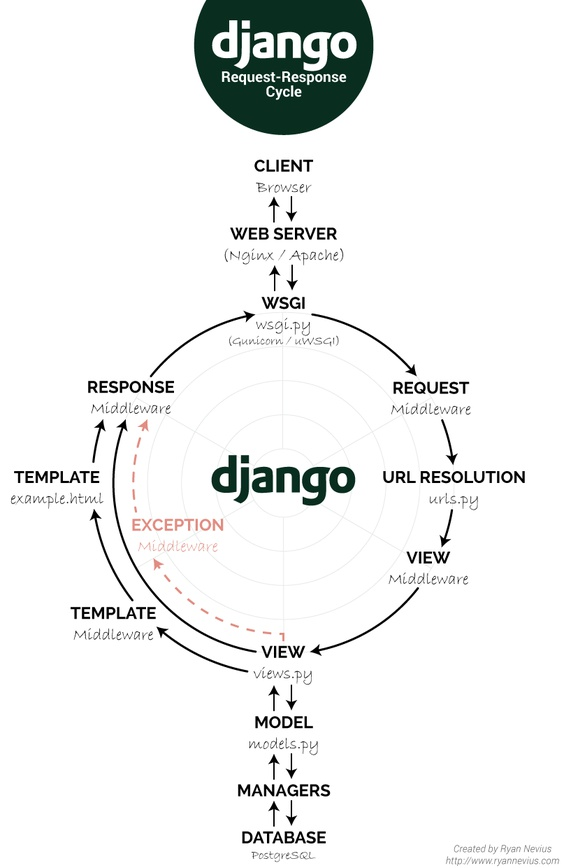
\includegraphics[width=0.5\columnwidth]{django-logo} 
    \caption{Funzionamento Django}
    \label{img:django-logo}
\end{figure}
Il codice riguardante il \textit{frontend} è sviluppato in linguaggio JavaScript, facendo uso del framework \grayname{React}\cite{prod:react} utilizzando come \textit{state container} \grayname{Redux}\cite{prod:redux}. La comunicazione tra \textit{frontend} e \textit{backend} è costituita da chiamate \glslink{rest}{REST} attraverso l'utilizzo di \grayname{Django REST framework}\cite{prod:django-rest-framework}. Per Python viene utilizzato \grayname{PyCharm}\cite{prod:PyCharm}, un \glslink{ide}{IDE} prodotto da JetBrains\textsuperscript{\textcircled{c}} che, oltre ad offrire un assistente "intelligente" per la scrittura di codice e \textit{safe refactoring}, include anche degli strumenti di sviluppo quali \textit{debugging} e \textit{deploying} su GitHub\cite{site:github}. Per quanto riguarda invece JavaScript, viene utilizzato \grayname{IntelliJ IDEA}\cite{prod:IntelliJ}, che offre le stesse funzionalità di \grayname{PyCharm}.

\section{Processi interni}
Il codice è organizzato all'interno di due repository GitHub\cite{site:github} ospitate nel profilo dell'azienda. In particolare, c'è una \textit{repository} per il versionamento del \textit{frontend} e una per quello del \textit{backend}. Lo sviluppo del codice avviene in rami separati per ogni sviluppatore; al compimento delle \textit{features} per una \textit{milestone} viene fatta una \textit{pull request} nel ramo \textit{development}. Quindi, dopo un periodo di test nel server di testing, viene fatta una \textit{pull request} nel ramo master e quindi il \textit{deploy} nell'ambiente di produzione.
\begin{figure}[H] 
    \centering
    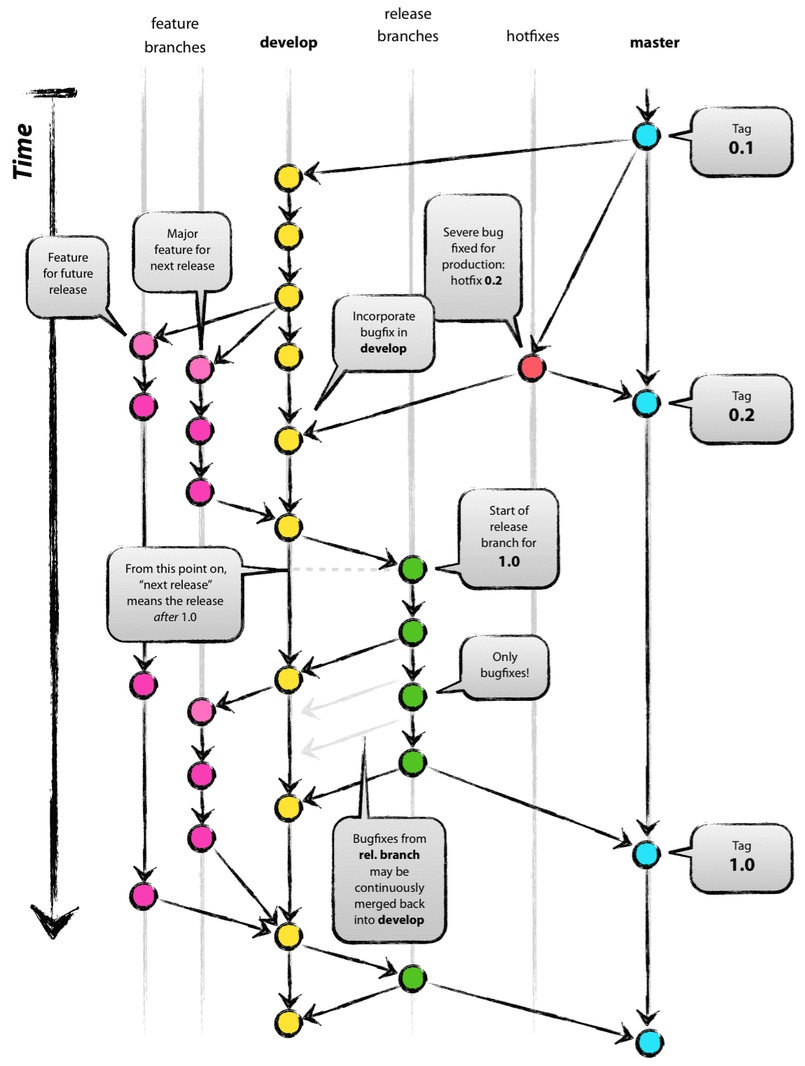
\includegraphics[width=0.5\columnwidth]{git-branches} 
    \caption{Distribuzione del lavoro su rami git}
    \label{img:git-branches}
\end{figure}
Il processo di verifica del codice è automatizzato da script interni che consentono una \textit{continuous integration}. Tali test vengono lanciati ogni volta che avviene un \textit{push} attraverso l'ausilio di \grayname{CircleCI}\cite{prod:circle-ci}, servizio che è integrato con GitHub e che ad ogni \textit{push} in automatico testa la \textit{build} in una macchina virtuale creata appositamente per i test.
\medskip
\\Invece, la gestione delle \textit{milestones} viene fatta attraverso i \textit{projects} di GitHub, in cui vengono fatti convogliare i rispettivi \textit{task} necessari per lo sviluppo delle \textit{features} selezionate. Ogni compito rappresenta un'azione atomica necessaria per l'implementazione della \textit{feature} ed è rappresentata da una \textit{issue} in GitHub. Ogni \textit{issue} viene quindi etichettata per tenere traccia del tipo di azione o priorità che identifica.


\section{Tipologia clientela}
La piattaforma viene principalmente utilizzata da professionisti del rischio, brokers e agenti assicurativi, che la utilizzano per reperire informazioni dettagliate sui i rischi assicurabili e per ricevere un preventivo in maniera istantanea di eventuali polizze.

\section{Innovazione}
RiskApp è una startup concentrata nell’innovazione del settore assicurativo, l’\textit{Insurtech}. Il tutto è nato dalla selezione in Unipol Ideas, il percorso di Open Innovation del Gruppo Unipol: un canale di dialogo e contaminazione con chi fa innovazione in ambiti collegati al core business aziendale. Unipol è tra i soci fondatori della Fondazione ItaliaCamp. Riskapp si è presentata in Expo Milano 2015 al Vivaio delle Idee, lo spazio dedicato all'innovazione ideato e gestito da Padiglione Italia, Ministero delle Politiche Agricole e Forestali e Fondazione ItaliaCamp\cite{site:riskapp-rai}. 
\medskip
\\Nel 2016 Unipol è diventata il primo cliente, inoltre sono state fatti altri programmi di accelerazione in Europa, tra i quali Deloitte Digital Disruptors\cite{site:deloitte-digital-startup} a Lisbona, MundiLab\cite{site:mundi-lab} a Madrid, Fintech Innovation Lab\cite{site:fintech} a Londra che hanno portato alla collaborazione con Società di consulenza quali Deloitte\cite{site:deloitte} e Accenture\cite{site:accenture}, riassicuratori Munich Re\cite{site:munich-re} e Swiss Re\cite{site:swiss-re}, e a nuovi clienti in Europa, come Fidelidade\cite{site:fidelidade} e P\&V\cite{site:pv}.


             	% L'azienda
% !TEX encoding = UTF-8
% !TEX TS-program = pdflatex
% !TEX root = tesi.tex
% !TeX spellcheck = it_IT

%**************************************************************
\chapter{Lo stage}
\label{cap:stage}
%**************************************************************

%\intro{Brevissima introduzione al capitolo}\\

%**************************************************************
\section{L'idea}
Lo stage è stato proposto durante l'incontro STAGE-IT\cite{site:stageit} tra le aziende e gli studenti di informatica e di ingegneria informatica. L'idea all'interno del quale si innesta lo stage proposto era la possibilità, da parte di un'agente assicurativo, di caricare una polizza assicurativa o il libretto e di poter ricavare, automaticamente, tutti i dati salienti in esso contenuti in maniera automatica. Quindi: ubicazioni, dimensioni, premi assicurativi, coperture, eccezioni, eccetera. 
\medskip
\\Dall'idea si è poi passati alla pratica: il primo passaggio sarebbe stato quello di creare un lettore \glslink{ocr}{OCR} di PDF per così dire "intelligente", che quindi fosse in grado di comprendere dove fossero posizionate le tabelle e il testo per poter poi analizzare le due tipologie di strutture dati in maniera differente e più efficace.

\section{Aspettative aziendali}
L'azienda RiskApp sperava, grazie allo stage, di poter iniziare a mettere "le mani in pasta" in un ambiente completamente non sondato del suo business. La possibilità di avere uno strumento del genere nel proprio portale le permetterebbe infatti di ampliare il \textit{set} di strumenti già in loro possesso, facilitando la navigazione e il reperimento delle informazioni da parte dell'utilizzatore. Inoltre ha un importante ruolo nella generazione di un database ordinato, all'interno del quale inserire tutte quelle informazioni specifiche che, se estrapolate a mano, avrebbero un costo proibitivo.

\section{Aspettative personali}
Ho affrontato l'evento STAGE-IT con il desiderio di poter trovare un'azienda che mi proponesse uno stage riguardante l'intelligenza artificiale. Fino ad allora mi ero solamente informato in maniera generica sull'argomento: volevo finalmente imparare a utilizzare gli algoritmi di \textit{machine learning} e \textit{deep learning} e capire come declinarli nell'ambito aziendale. Invero, tra le oltre 80 aziende e molte più offerte di stage, solo due o tre offrivano questa possibilità e RiskApp mi ha convinto per il fatto che è una realtà giovane - è ancora registrata come StartUp. Ero infatti anche molto incuriosito dall'idea di azienda fortemente dinamica.

\section{Obiettivi}
Gli obiettivi stilati ad inizio stage erano molto audaci e, sebbene questo abbia portato la ridefinizione del piano di lavoro in corso d'opera, ha aiutato l'azienda a capire la complessità dell'argomento e spronato me a velocizzare il più possibile il processo conoscitivo e produttivo.
\medskip
\\Dagli obiettivi presentati dall'azienda ho estrapolato dei requisiti, che seguiranno le seguenti notazioni:
\begin{itemize}
    \item \textbf{O} per gli requisiti obbligatori;
    \item \textbf{D} per gli requisiti desiderabili, quindi non vincolanti ma dal valore aggiuntivo;
    \item \textbf{F} per gli requisiti facoltativi
\end{itemize}
Nella tabella ogni notazione sarà seguito da un numero, per poter identificare ogni obiettivo univocamente.\\

{
    \def\arraystretch{2}\tabcolsep=10pt
\begin{table}[H]
    \small
    \begin{tabular}{ |p{2cm} |p{11cm}|}
        \hline
        \textbf{ID} & \textbf{Descrizione} \\ \hline
        
        \multicolumn{2}{|c|}{\textbf{Obbligatori}} \\ \hline
        
        O01 & Creazione di un algoritmo che faciliti la creazione di un dataset per allenare una rete neurale \\ \hline
        O02 & Creazione di una struttura di testing per la valutazione visiva dei risultati ottenuti \\ \hline
        O03 & Creazione di un algoritmo di estrazione di informazioni mirate da un libretto assicurativo \\ \hline
        O04 & Gestione di tutti gli algoritmi il più automatica possibile, possibilmente tramite l'uso di costanti \\ \hline
        O05 & Utilizzo del linguaggio Python versione 3 \\ \hline
        
        \multicolumn{2}{|c|}{\textbf{Desiderabili}} \\ \hline
        
        D01 & Creazione di un batch multithreading per l'estrazione parallela di informazioni da più polizze \\ \hline
        
        \multicolumn{2}{|c|}{\textbf{Facoltativi}} \\ \hline
        
        F01 & Integrazione del sistema nell'infrastruttura dell'azienda \\ \hline
        
    \end{tabular}
    \caption{Tabella degli obiettivi}
\end{table}
}
    
   
\section{Analisi preventiva dei rischi}
Durante la fase iniziale ho individuato alcuni possibili rischi che questo progetto mi avrebbe potuto portare ad affrontare, consentendomi di elaborare una strategia di conseguenza:

{
    \def\arraystretch{2}\tabcolsep=10pt
    
\begin{table}[H]
    \small
    \begin{tabular}{ |p{4.5cm} |p{4.5cm} |p{3cm}|}
        \hline
        \textbf{Descrizione} & \textbf{Piano di emergenza} & \textbf{Rischio} \\ \hline
        \textbf{Non conoscenza del linguaggio}: prima di iniziare lo stage non avevo mai programmato in Python. &
        Escogitare dei meccanismi di apprendimento rapido del linguaggio, tramite corsi online e provando fin da subito a scrivere del codice per conto proprio.
        \newline
        Chiedere agli altri stagisti qualche domanda più tecnica che mi potesse risparmiare del tempo per la ricerca. & 
        Occorrenza: Alta \newline Pericolosità: Media \\
        \hline
        
        \textbf{Non conoscenza della materia}: Prima dell'inizio dello stage la conoscenza teorica in mio possesso di \textit{machine learning}, \textit{deep learning} e di reti neurali era generale e per niente applicata. &
        Frequentare il prima possibile dei corsi specializzanti. &
        Occorrenza: Alta \newline Pericolosità: Alta \\ 
        \hline
        
        \textbf{Non conoscenza degli strumenti}: Per il \textit{machine learning} e il \textit{deep learning} esistono tutta una serie di strumenti già pronti all'uso che risparmiano molto tempo in fase di progettazione e codifica. &
        Mettere mano il prima possibile a questa strumentazione, così da entrare in confidenza fin da subito con le tecnologie e familiarizzare con le personalizzazioni che si possono adoperare. &
        Occorrenza: Alta \newline Pericolosità: Media \\
        \hline
        \textbf{Esami durante il lavoro}: Lo stage è iniziato senza avere la certezza di aver superato un esame, che avrei dovuto quindi sostenere durante il periodo di lavoro. &
        Pianificare il lavoro in maniera tale da lasciare fasi meno impegnative della programmazione - come la fase di test - nel periodo subito precedente l'esame. Così la sera sarei riuscito a studiare. &
        Occorrenza: Alta \newline Pericolosità: Bassa \\
        \hline
    \end{tabular}
    \caption{Tabella dell'analisi dei rischi}
\end{table}
}


\section{Pianificazione}
Dopo un'analisi approfondita degli obiettivi richiesti dall'azienda, dopo essermi reso conto dei rischi e in accordo col tutor aziendale, ho capito che la pianificazione avrebbe dovuto comprendere un numero di ore molto alto per la formazione prima di poter iniziare a sviluppare l'applicazione vera e propria. 
\medskip
\\Ho intuito immediatamente poi che la creazione di una "catena di montaggio" sarebbe stata da preferire rispetto ad un approccio monolitico. Questo mi avrebbe permesso di capire più rapidamente il funzionamento di ogni singola parte della \textit{pipeline} (di cui si discuterà in sezione \ref{cap:progettazione}), potendola quindi testare e migliorare man mano grazie ai risultati ottenuti da altre parti della catena. L'effetto collaterale di questo approccio è che il risultato finale, dato dall'assemblaggio dei vari pezzi, sarebbe arrivato più tardi di quanto un approccio monolitico avrebbe potuto offrire.

{
    \def\arraystretch{2}\tabcolsep=10pt
\begin{table}[H]
    \small
    \begin{tabular}{ |p{2cm} |p{10cm}|}
        \hline
        \textbf{Ore} & \textbf{Descrizione dell'attività} \\ \hline
        
        24 & Raccolta informazioni e definizioni dei requisiti del progetto; \\ 
        \hline
        100 & Formazione su:
        \begin{itemize}
            \item python;
            \item openCV;
            \item algoritmi di \textit{machine learning} e \textit{deep learning} e loro ottimizzazione;
            \item basi di \grayname{Tensorflow};
            \item basi di \grayname{Keras}.
        \end{itemize}\\ 
        \hline
        40 & Creazione della struttura per l'allenamnto di reti neurali; \\ \hline
        80 & Creazione di un algoritmo per l'estrazione di dati dai documenti; \\ \hline
        24 & Creazione di test automatici per la valutazione visiva di una rete neurale; \\ \hline
        18 & (Desiderabile) Creazione di un batch multithreading per un'analisi estensiva su più polizze; \\ \hline
        18 & (Facoltativo) Integrazione nell'infrastruttura aziendale. \\ \hline
        
        \multicolumn{2}{|c|}{\textbf{Totale: 304 ore}} \\ \hline
        
    \end{tabular}
    \caption{Tabella della suddivisione delle ore}
\end{table}
}             		% Processi
% !TEX encoding = UTF-8
% !TEX TS-program = pdflatex
% !TEX root = tesi.tex
% !TeX spellcheck = it_IT

%**************************************************************
\chapter{La teoria}
\label{cap:teoria}
Per comprendere al meglio le tecnologie e i concetti che avrei dovuto implementare in questo stage ho deciso di avere un approccio il più sistematico possibile alla materia. Essendo la teoria implicata molto ampia e con un approccio matematico non banale, ho deciso inizialmente di leggermi molti articoli, per lo più tratti da \textit{medium.com}\cite{site:medium}, ottimo sito di divulgazione generale. Dopodiché ho frequentato alcuni corsi su Coursera\cite{site:coursera}, famoso sito di corsi online.
\medskip
\\In particolare, ho seguito buona parte del corso sul \textit{machine learning}\cite{course:machine-learning} tenuto da Andrew Ng\cite{person:andrew-ng} per avere un'infarinatura generale di cosa vuol dire questo approccio matematico. In seguito per avere un'idea più completa riguardo le \textit{deep networks} mi sono affidato a dei corsi, sempre su Coursera\cite{site:coursera} e tenuti dallo stesso docente, che fanno parte di una specializzazione\cite{course:deep-learning-specialization}. In particolare, ho completato - con certificato - i seguenti corsi:
\begin{itemize}
	\item Neural Networks and Deep Learning\cite{course:neural-networks-deep-learning};
	\item Improving Deep Neural Networks: Hyperparameter tuning, Regularization and Optimization\cite{course:improving-nn};
	\item Structuring Machine Learning Projects\cite{course:structuring-ml-proj};
\end{itemize}
Non sono invece riuscito a concludere gli esercizi finali del quarto capitolo: Convolutional Neural Networks\cite{course:cnn}.
\medskip
\\Tutta questa preparazione mi è stata di fondamentale aiuto per comprendere le tecnologie che sarei andato ad utilizzare di lì a breve, nonché mi ha dato la possibilità di ampliare enormemente la mia conoscenza al riguardo. Nei capitoli seguenti descriverò in maniera più intuitiva che matematica le tecnologie che ho esplorato.

%**************************************************************

%\intro{Brevissima introduzione al capitolo}\\

%**************************************************************
\section{Cos'è l'apprendimento automatico}
L'apprendimento automatico - in inglese \textit{machine learning} - si basa sull'idea che un algoritmo sia capace di dire qualcosa di interessante riguardo un insieme di dati senza la necessità, da parte di un utente, di dover scrivere alcuna riga di codice specifico sul problema.\cite{site:machine_learning_is_fun} L'algoritmo infatti, sulla base di questi dati, è capace di sviluppare una propria logica. Prendiamo ad esempio due task:
\begin{itemize}
	\setlength\itemsep{0em}
	\item riconoscere dei numeri scritti a mano;
	\item riconoscere una mail di spam da una legale.
\end{itemize}
Possiamo sfruttare lo stesso algoritmo di apprendimento automatico per generare due logiche differenti solamente a partire da due \gls{set} di dati diversi.


\subsection{Apprendimento supervisionato e non supervisionato}
Esistono due principali categorie di apprendimento automatico: supervisionato e non supervisionato.\cite{site:supervised_vs_unsupervised_learning}

\subsubsection*{Apprendimento supervisionato}
Il \textit{supervised learning} è principalmente usato per la classificazione, dove vogliamo ottenere delle etichette a partire da dati in ingresso, oppure per la regressione, dove l'input è mappato in un output continuo. In entrambi gli aspetti, l'obiettivo è quello di dedurre una particolare relazione o struttura nei dati di input che ci permetta di produrre un output corretto.

\subsubsection*{Apprendimento non supervisionato}
Con l'\textit{unsupervised learning} si vuole trarre una struttura a partire da dati in ingresso senza fornire esplicitamente un'etichetta. Si usa principalmente per il raggruppamento e le stime di densità di un insieme di dati in input.



\section{Le reti neurali}
Le reti neurali sono una classe di modelli di apprendimento automatico che hanno rivoluzionato il mondo del \textit{machine learning}.
Lo sviluppo delle \textit{neural networks} è stata la chiave per insegnare ad una macchina a \textit{capire} come un umano. 

\subsection*{Cos'è una rete neurale}
La rete neurale si può pensare come una funzione composta. Essa accetta alcuni tipi di input e genera degli output. I componenti della rete neurale sono i \textbf{neuroni} (anche detti \textit{Perceptrons} oppure unità), che a loro volta sono una funzione che utilizza \textbf{pesi} (o anche detti connessioni) e \textbf{\textit{biases}}. Viene poi interpellata una \gls{funzione di attivazione} non lineare per restringere l'output ad un certo intervallo. Se ne immaginassimo una di combinazione lineare:
\[f(x_1, x_2)=W_1*x_1 + W_2*x_2 + b\]
allora il neurone sarebbe la funzione, $W_1$ e $W_2$ sarebbero i pesi e $b$ il \textit{bias}.
I neuroni sono organizzati in strati - altresì chiamati \textit{layers} - e il numero di neuroni all'interno di ogni strato è a carico del creatore. Tuttavia, troppo strati per un compito semplice porta ad aumentare la complessità della rete senza motivo e a diminuirne l'accuratezza. \'E ovviamente vero anche il contrario. Per ogni strato, l'output di un neurone viene utilizzato come input per un altro neurone in un altro strato.
\medskip
\\Ogni rete ha due tipologie di strati: lo strato per l'input (che non ha alcun tipo di computazione al suo interno) e quello per l'output. Tutti gli altri \textit{layers} che sono tra questi due sono chiamati nascosti. Nell'immagine \ref{img:nn} si può notare una rete neurale composta da uno strato di input con otto unità, uno di output con 4, tre nascosti con 9 unità ciascuno. Una rete neurale con più di due strati nascosti è definita profonda.
\begin{figure}[!h] 
    \centering 
    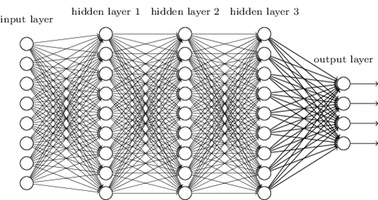
\includegraphics[width=0.9\columnwidth]{nn} 
    \caption{Una rete neurale profonda}
    \label{img:nn}
\end{figure}

\subsection*{Come la rete impara}
La rete impara attraverso l'analisi della sua \textit{loss function}. La \textit{loss function} è una funzione che ci dice quanto la nostra rete è buona per un determinato compito. Per capirlo intuitivamente, essa prende ogni dato in input, lo computa attraverso la rete neurale, lo si sottrae al numero che ci aspettiamo sia il risultato e ne prendiamo il quadrato. Dati quindi $y$ il numero che ci aspettiamo, $\hat{y}$ il numero che otteniamo dalla computazione della rete, $i$ l'indice dell'esempio che stiamo prendendo in considerazione: 
\[L(y, \hat{y})=\frac{1}{m}\sum_{i=1}^{m}(y_i - \hat{y}_i)^2 \]
otteniamo la "distanza" dal risultato che vorremmo ottenere. Imparare diventa quindi un problema di minimo, ovvero vogliamo trovare un risultato che minimizzi la \textit{loss function}. A questo scopo si utilizzano la discesa del gradiente e la \textit{backward propagation}

\subsubsection*{Discesa del gradiente}
Il metodo di discesa del gradiente è una tecnica che consente di determinare i punti di massimo e di minimo di una funzione a più variabili.
\\Pensando ad una funzione $f(x)$ con $x\in \Re^n$, la direzione di massima discesa (ovvero la direzione verso la quale la funzione "scende" più rapidamente) in un punto $\bar{x}$ è dato dall'opposto del suo gradiente in quel punto, ovvero: $p_k:=-\nabla f(\bar{x})$. Questa scelta garantisce che la soluzione tenda ad un punto di minimo di $f$. Il metodo del gradiente prevede dunque di partire da una soluzione iniziale $x_0$ scelta arbitrariamente e di procedere in maniera iterativa aggiornandola come:
\[x_{k+1} = x_k + \alpha_kp_k\]
dove $\alpha_k\in \Re^+$ corrisponde alla lunghezza del passo di discesa, la cui scelta diventa quindi cruciale nel determinare la velocità con cui l'algoritmo converge alla soluzione richiesta.

\subsubsection*{\textit{Backward propagation}}
La propagazione all'indietro viene utilizzata dagli algoritmi di discesa del gradiente per aggiustare i pesi dei neuroni calcolando il gradiente della \textit{loss function}. In pratica, l'algoritmo di ottimizzazione di una rete neurale ripete un ciclo costituito da due fasi: propagazione e aggiornamento dei pesi. Quando un vettore in input viene dato in pasto alla rete, viene propagato "in avanti" attraverso la rete, strato su strato, fino a che raggiunge lo strato di uscita. A questo punto l'output viene paragonato col risultato aspettato usando una \textit{loss function}. A questo punto, l'errore che è risultato viene calcolato per ognuno dei neuroni dello strato di output, dopodiché viene propagato dallo strato di uscita all'indietro nella rete, fino ad associare a tutti i neuroni un valore d'errore che riflette il loro contributo all'output originale. 
\medskip
\\La \textit{backpropagation} quindi usa questi valori per calcolare il gradiente della \textit{loss function}. Nella seconda fase, questo gradiente viene dato in pasto al metodo di ottimizzazione, che lo usa per aggiornare i pesi, per cercare di minimizzare la funzione di perdita.

\medskip
\medskip
\medskip
Per il mio studio mi sono fin da subito concentrato sulle \textit{deep neural network}, ovvero reti neurali che sono composte da molti strati che comunicano fra loro. Nelle prossime sezioni mostrerò alcuni modelli ben definiti e le architetture che poi ho usato nel mio progetto.



\section{Excursus sulle \textit{deep network architectures}}
Quasi tutto il progresso sull'apprendimento profondo degli ultimi anni per la branca del \textit{computer vision} può essere riassunto in poche architetture di reti neurali.
Tralasciando in questa sede tutta la matematica e il codice che vi sta dietro, vorrei introdurre il lettore a comprendere come queste reti funzionano e perché.
\medskip
\\Prendiamo ad esempio la libreria Keras\cite{prod:keras}: questa libreria, capace di lavorare come \textit{wrapper} attorno a \grayname{Tensorflow}\cite{prod:tensorflow}, \grayname{CNTK}\cite{prod:CNTK} e \grayname{Theano}\cite{prod:Theano} offre sei modelli già allenati, \textit{built-in} al suo interno:
\begin{itemize}
	\item \textbf{VGG16}
	\item \textbf{VGG19}
	\item \textbf{MobileNet}
	\item \textbf{ResNet50}
	\item \textbf{Inception v3}
	\item \textbf{Xception}
\end{itemize}

Le reti VGG seguono l'archetipo - ora in parte superato - delle \textit{convolutionary nets}: sono costituite infatti da una serie di strati convoluzionali, di \gls{max-pooling} e con uno strato \textit{fully-connected} per classificazione nel fondo. Le MobileNet sono una versione ottimizzata per le applicazioni mobile della Xception. Le ultime tre, invece, ridefiniscono veramente il modo in cui pensiamo alle reti neurali.
\medskip

\subsection{ResNet}
La domanda chiave che gli sviluppatori si sono fatti pensando al modello di questa rete è stata: \textit{Perché ogni rete profonda ha una prestazione peggiore man mano che si aggiungono strati?}\cite{site:intuitive_guide_DNN_architecture}
Infatti ci si può aspettare che, dati $n$ strati, una rete con $n+1$ abbia la stessa identica accuratezza di quella a $n$. Tuttavia la pratica smentisce questa osservazione, mettendo in risalto l'opposto.
\medskip
\\L'ipotesi che gli autori di ResNet hanno fatto è stata che \textit{mappings} diretti sono difficili da imparare. Così hanno proposto una modifica: al posto di cercare di stimare una funzione $G$ che dato un $x$ restituisca $G(x)$, è meglio apprendere la \textit{differenza} tra i due - anche chiamato residuo, da cui il nome. Di conseguenza, per calcolare $G(x)$ a partire da $x$ basta aggiungere il suo residuo.\\
Quindi, detto:
\[F(x)=G(x)-x\]
il nostro residuo, al posto di apprendere $G(x)$ direttamente, la rete cercherà di imparare
\[F(x)+x\].
Questo ci dà l'opportunità di introdurre il \textit{ResNet block} (figura \ref{img:resnet_block}):
\begin{figure}[!h] 
	\centering 
	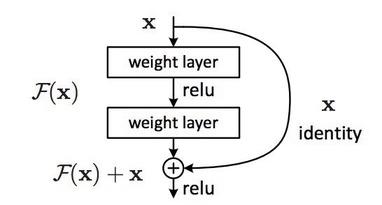
\includegraphics[width=0.9\columnwidth]{resnet_block} 
	\caption{Blocco ResNet}
	\label{img:resnet_block}
\end{figure}
ogni blocco è costituito da una serie di strati e da una "scorciatoia", che aggiunge l'input del blocco stesso al suo output. L'operazione di aggiunta è fatta per ogni elemento, e se input e output sono di dimensioni diverse viene eseguito un \textit{\gls{zero-padding}} oppure una proiezione (via \gls{convoluzioni} 1x1) per portare l'input alla stessa dimensione dell'output. Intuitivamente è molto più semplice imparare mandando $F(x)$ a 0 lasciando l'output a $x$ piuttosto di cercare di imparare una trasformazione identità da zero. In altre parole, ResNet dà uno strato di riferimento - $x$, per l'appunto - da cui iniziare ad imparare.
\medskip
\\Quest'idea funziona molto bene nella pratica. Mentre i modelli precedenti soffrivano del cosiddetto \gls{vanishing gradient}, qui invece si possono sfruttare delle scorciatoie verso gli strati precedenti: reti da 50, 100 o addirittura 1000 strati di profondità hanno ancora delle ottime performance.

\subsection{Inception}
La domanda chiave che invece gli sviluppatori della famiglia delle Inceptions si sono fatti è stata: \textit{come possiamo scalare efficientemente le reti neurali senza aumentare il costo computazionale?}\cite{site:intuitive_guide_DNN_architecture} 
Il paper originale\cite{site:inception} si concentra sulla definizione di un "Inception module", che ha come base due concetti fondamentali: le operazioni sugli strati e la possibile riduzione della dimensione di ognuno. Ma andiamo con ordine:

\subsubsection*{Più operazioni per strato}
In una \textit{conv net} tradizionale ogni livello estrae nuove informazioni dallo strato precedente per trasformare i dati in ingresso in una rappresentazione più fruibile per la rete. Tuttavia, ogni tipologia di livello estrae informazioni diverse: l'output di una convoluzione di dimensione 5x5 è diverso da quello di uno a 3x3, ed è diverso anche da uno dove si opera un \textit{max-pooling}. Come possiamo sapere se una certa trasformazione in un certo strato sta estraendo informazioni utili?
\medskip 
\\L'idea è stata di lasciare la rete decidere quali scegliere: il modulo Inception esegue multiple e diverse trasformazioni sullo stesso input in maniera parallela, concatenando poi i risultati in un output singolo. In pratica, come mostrato in figura \ref{img:inception_module}, per ogni strato Inception esegue una convoluzione 5x5, 3x3 e un \textit{max-pooling}. Lo strato successivo si occupa quindi di decidere se e come usare ogni informazione così tracciata.
\begin{figure}[!h] 
	\centering 
	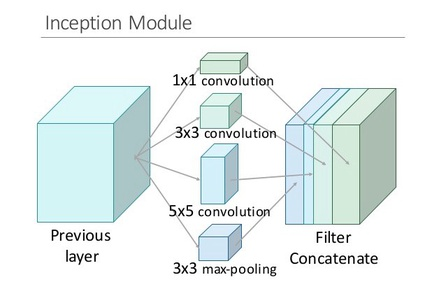
\includegraphics[width=0.9\columnwidth]{inception_module} 
	\caption{Modulo Inception}
	\label{img:inception_module}
\end{figure}

\subsubsection*{Riduzione dimensionale}
Facendo così tuttavia si introduce un problema: si è ingrandita drasticamente la computazione. Per ogni filtro aggiunto bisogna fare la convoluzione di tutti gli strati di input precedenti per calcolare un singolo output. Questo porta ad un aumento quadratico o addirittura maggiore del numero dei filtri per strato. Ci si rende facilmente conto che questo non è sostenibile.
\medskip
\\Ecco quindi la soluzione: gli autori hanno pensato ad una convoluzione 1x1 per "filtrare" la profondità degli output. Se si considera una convoluzione 1x1 su un singolo strato si ha una valutazione di un valore alla volta. Tuttavia, vista su più \gls{canali}, essa può estrarre informazioni "spaziali" e comprimerli ad una dimensione inferiore. Facciamo un esempio: usando 20 filtri 1x1, un input di dimensione 64x64x100 può essere compresso a 64x64x20. Così facendo gli autori del modello sono stati capaci di allocare più trasformazioni per strato in parallelo, avendo una rete simultaneamente ampia (per via del parallelismo) e profonda (grazie al grande numero di strati).
\begin{figure}[H] 
	\centering
	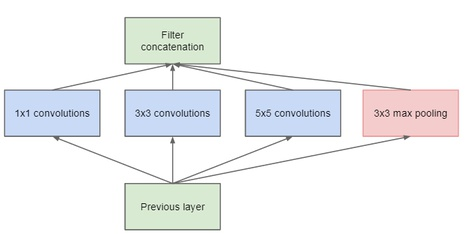
\includegraphics[width=0.6\columnwidth]{inception_module_naive} 
	\caption{Concezione iniziale del modulo Inception}
	\label{img:inception_module_naive}
\end{figure}
\begin{figure}[H] 
	\centering
	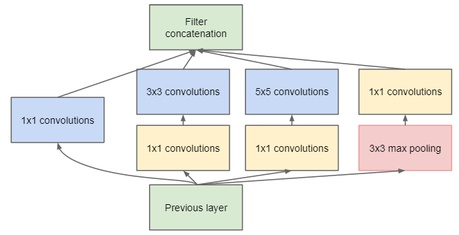
\includegraphics[width=0.6\columnwidth]{inception_module_reduced} 
	\caption{Modulo Inception con riduzione}
	\label{img:inception_module_reduced}
\end{figure}
Inception ha dimostrato la potenza delle architetture composte da "reti dentro a reti", aggiungendo un altro gradino importante alla potenza rappresentale delle reti neurali.
\begin{figure}[H] 
	\centering
	
\includegraphics[width=0.6\columnwidth]{need_go_deeper} 
	\caption{Meme letteralmente citato dall'articolo originale su Inception}
	\label{img:need_go_deeper}
\end{figure}

\subsection*{Xception}
Xception sta per \textit{extreme inception} e porta il concetto del modulo Inception ad un estremo. L'ipotesi da cui si sviluppa questa rete è: \textit{la correlazione tra i canali e quella spaziale sullo stesso frame è sufficientemente bassa da poter preferire di non mapparli assieme}.
Cosa vuol dire? Nelle tradizionali reti a convoluzione, gli strati cercano correlazioni sia in profondità che in larghezza (ovvero sullo stesso frame). Con Inception si ha avuta una prima separazione: usando una convoluzione 1x1 si può mappare l'input originale in vari input separati, sui quali poi poter eseguire diversi tipi di trasformazione. Xception porta il concetto un po' oltre: al posto di partizionare l'input in tanti piccoli pezzi, questa partiziona ogni canale separatamente, quindi esegue una convoluzione 1x1 in profondità per catturare correlazioni tra i canali.
\begin{figure}[H] 
	\centering
	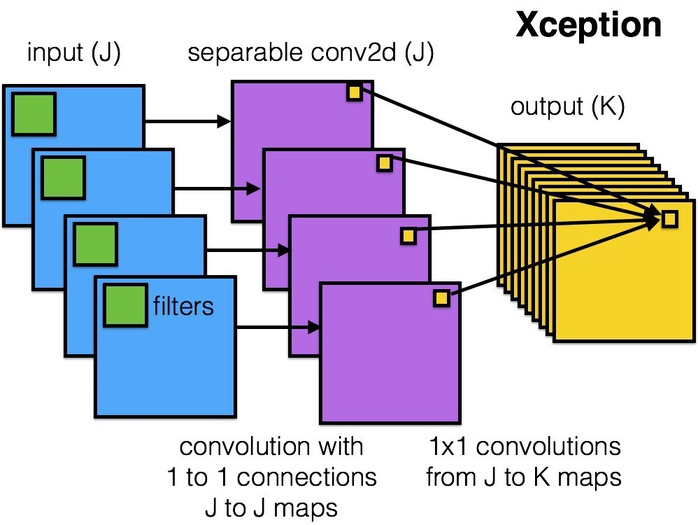
\includegraphics[width=0.6\columnwidth]{xception} 
	\caption{Modulo Xception}
	\label{img:xception_module}
\end{figure}
Possiamo immaginare questa operazione considerando la ricerca di correlazione tra spazi bidimensionali e poi su unidimensionali. Il che è intuitivamente più semplice che cercarle in uno spazio direttamente tridimensionale.
\medskip
\\Questo modello è molto recente - è uscito nell'aprile del 2017 - e già ha risultati promettenti, soprattutto per quanto riguarda l'efficienza computazionale con un più alto numero di \gls{classi} da analizzare.


\section{Il \textit{deep learning} applicato all'\textit{object detection}}
Con l'aumento delle auto a guida autonoma, dei sistemi di videosorveglianza \textit{smart}, del riconoscimento facciale e di molti altri campi di utilizzo, la richiesta di sistemi di  \textit{detection} è andata via via sempre aumentando. Tuttavia, questi sistemi non solo richiedono di classificare ogni oggetto in un'immagine, ma anche di trovarlo, disegnandogli un rettangolo attorno. Come si può immaginare, questo compito è nettamente più complesso della semplice \textit{image classification}. Fortunatamente i migliori approcci usati oggi giorno provengono principalmente da estensioni dei modelli già esistenti e derivati dalla classificazione.
%\vspace{1.5\baselineskip}
\medskip
\\Circa un anno fa Google ha rilasciato una nuova \glslink{api}{API} di \textit{object detection} e, assieme ad essa, ha fornito anche una serie di architetture - con i relativi pesi già allenati - per alcuni specifici modelli:
\begin{itemize}
	\item Single Shot Multibox Detector (SSD) con le MobileNets
	\item SSD con Inception V2
	\item Region-Based Fully Convolutional Networks (R-FCN) con Resnet 101
	\item Faster R-\glslink{cnn}{CNN} con Resnet 101
	\item Faster \glslink{rcnn}{R-CNN} con Inception Resnet v2
\end{itemize}
Dopo aver intrapreso uno studio preliminare riguardo le varie architetture, ho preferito concentrarmi su due in particolare: la Faster R-CNN con Inception Resnet V2 e la SSD con Inception V2. Queste infatti sono disponibili all'interno dell'API di \textit{object detection}\cite{prod:tensorflow_o_d_api} di \grayname{Tensorflow}\cite{prod:tensorflow} e hanno reso il mio approccio alla materia molto meno drastico.

\subsection{Cosa sono il \textit{transfer learning} e il \textit{fine tuning}}
Per usufruire di queste reti ho dovuto utilizzare il \textit{transfer learning}. Molte poche persone allenano un'intera \textit{conv net} da zero con inizializzazione casuale, poiché è raro avere a disposizione un \textit{dataset} così ampio. Piuttosto, si tende ad utilizzare una rete già allenata. quindi usare i pesi - ovvero le informazioni che già ha imparato da un particolare insieme di dati - di questa come di partenza per la propria. 
\medskip
\\In particolare, per questo progetto ho utilizzato il \textit{fine tuning}: \grayname{Tensorflow} mette a disposizione i pesi "congelati" di tutti gli strati eccetto del penultimo. Così facendo, possiamo allenare la nostra rete ad imparare la rappresentazione del solo ultimo strato, utilizzando il \textit{dataset} personale. Questo è ovviamente possibile solamente se c'è una certa continuità dell'obiettivo della rete: sfruttare il \textit{fine tuning} per imparare una voce utilizzando come base di partenza il grafo di una \textit{object detection} è inutile e controproducente.

\subsection{Faster R-CNN}
La Faster R-CNN è l'architettura di riferimento nell'apprendimento profondo, in particolare per quanto riguarda l'\textit{object detection} ed è di riferimento per altre architetture, in particolare anche per la SSD. Tuttavia, non la si può realmente capire se prima non si dà una rapida occhiata alle sue predecessore, la R-CNN e la Fast R-CNN.

\subsubsection*{R-CNN}
La R-CNN, ovvero la \textit{Region-based Convolutional Neural Network} consiste di tre passaggi:
\begin{enumerate}
	\item scansiona l'immagine di input e cerca oggetti possibili con un algoritmo di ricerca selettiva, generando circa 2000 \textit{region proposal}, regioni da "proporre" agli strati successivi;
	\item esegue una rete convoluzionale su ognuna di esse;
	\item prende l'output di ogni CNN e lo dà in pasto a:
	\begin{itemize}
		\item una \glslink{svm}{SVM} per classificare le regioni;
		\item una \gls{regressione lineare} per creare un riquadro attorno all'oggetto, se esiste.
	\end{itemize}
\end{enumerate}
Gli step sono mostrati nella figura \ref{img:r-cnn_architecture}.
\begin{figure}[H] 
	\centering
	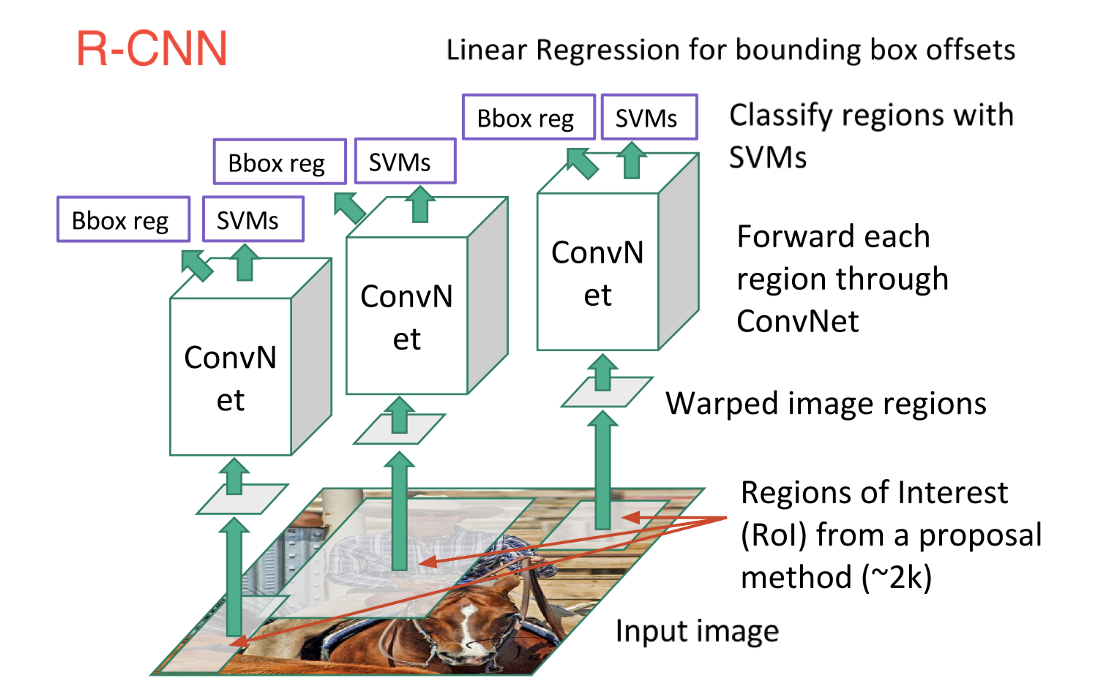
\includegraphics[width=0.9\columnwidth]{r-cnn} 
	\caption{Architettura R-CNN}
	\label{img:r-cnn_architecture}
\end{figure}
Intuitivamente, prima di tutto si trovano le possibili regioni in cui può essere contenuto un oggetto, poi si estraggono le informazioni ad esse associate, poi in base a queste si classificano. Si è trasformato un problema di \textit{object detection} in uno di classificazione: era un approccio molto intuitivo ma allo stesso tempo lento e oneroso.

\subsubsection*{Fast R-CNN}
Questa architettura è stata la diretta discendente della R-CNN, ma ha aumentato la sua velocità con due fattori chiave:
\begin{itemize}
	\item esegue l'estrazione di informazioni una volta prima di creare le regioni da proporre; così facendo può permettersi di eseguire una sola CNN al posto di doverne eseguire una per ogni regione;
	\item sostituisce la SVM con un \textit{layer} \gls{softmax}.
\end{itemize}
La nuova architettura si mostrava quindi come in figura \ref{img:fast-r-cnn_architecture}.
\begin{figure}[!ht] 
	\centering
	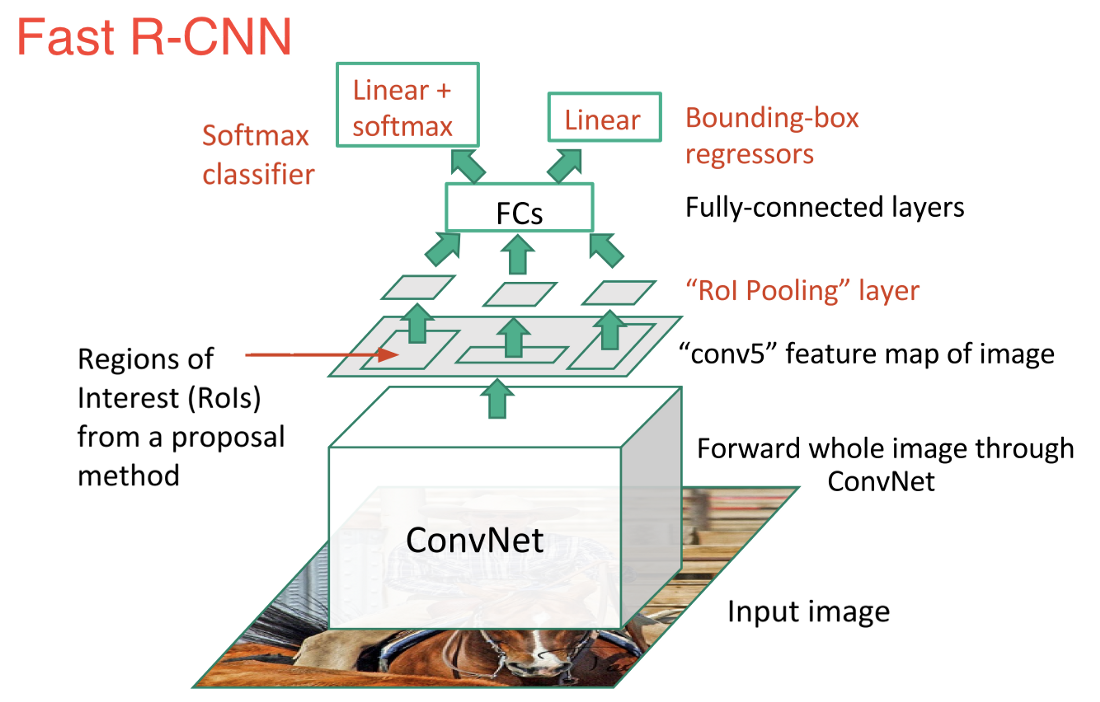
\includegraphics[width=0.9\columnwidth]{fast-r-cnn} 
	\caption{Architettura Fast R-CNN}
	\label{img:fast-r-cnn_architecture}
\end{figure}
Come si può vedere in figura, le \textit{region proposals} sono generate a partire dall'ultimo strato di informazioni ricavate dalla rete e non dall'immagine in sé. \'E quindi possibile allenare una singola CNN per l'immagine intera. Inoltre, al posto di usare molte SVM per classificare ogni classe, c'è un solo \textit{layer} \textit{softmax} che genera una probabilità diretta.
\medskip
\\La Fast R-CNN era molto più veloce della precedente, ma l'algoritmo di \textit{selective search} era ancora troppo lento.

\subsubsection*{Faster R-CNN}
Per risolvere questo ultimo collo di bottiglia si è adottato, al posto dell'algoritmo di ricerca selettiva, una rete neurale veloce. In particolare, una RPN, \textit{Region Proposal Network}:
\begin{itemize}
	\item viene generata una \textit{sliding window} di dimensione 3x3 posizionata sull'ultimo strato della CNN iniziale, che si muove lungo la mappa e ne restituisce una versione più piccola, ridotta (ad esempio a 256-d);
	\item per ogni \textit{sliding window} genera più possibili regioni basate su alcune \textit{boxes} di proporzione prestabilita;
	\item ogni regione proposta consiste di:
	\begin{itemize}
		\item un punteggio, \textit{score}, col quale viene valutata la \textit{box} trovata;
		\item le effettive quattro coordinate della scatola;
	\end{itemize}
\end{itemize}
In altre parole, si guarda in ogni posto proposto dall'ultimo strato della \textit{conv net}, si considerano $k$ diverse scatole centrate su ognuna di esse: una alta, una larga, una grande, una piccola, ecc. Per ognuna di queste viene generato un punteggio, una sorta di \textit{likelihood}. 
Da notare, infine, che anche se la RPN ha come output delle \textit{bounding boxes}, essa non aspira a classificare un potenziale oggetto: semplicemente propone delle regioni in cui ci potrebbe essere. Se una scatola ha un punteggio sufficiente, viene quindi passata avanti come \textit{region proposal}.
\begin{figure}[!ht] 
	\centering
	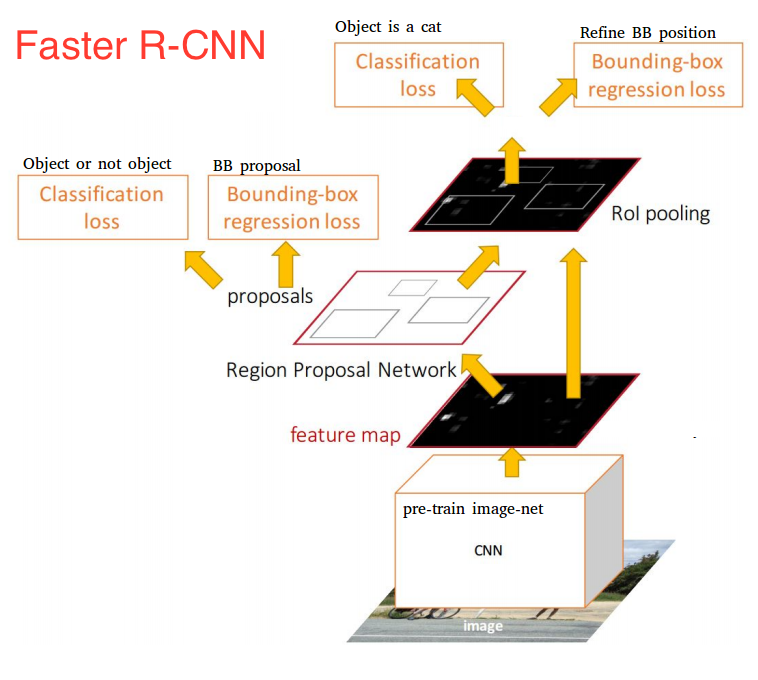
\includegraphics[width=0.7\columnwidth]{faster-r-cnn} 
	\caption{Architettura Faster R-CNN}
	\label{img:faster-r-cnn_architecture}
\end{figure}

\subsection{SSD}
Mentre la Faster R-CNN prima generava delle regioni, per poi usare un \textit{fully connected layer} per classificarle, la SSD fa tutto questo in un solo colpo. Da qui il nome, Single-Shot Detector.
In pratica, data un'immagine appartenente ad un \textit{set} con delle \textit{ground truth label}, ovvero delle immagini etichettate, la SSD fa questi passaggi:
\begin{enumerate}
	\item prima passa l'immagine attraverso una serie di strati convoluzionali, raggruppando più insiemi di mappe con informazioni a diverse misure (ad esempio 10x10, poi 6x6, e così via);
	\item per ogni \textit{location}, per ognuna delle \textit{feature maps}, usa un filtro con una convoluzione 3x3 per valutare insiemi più piccoli di scatole; questo è più o meno quello che viene fatto con le scatole della Faster R-CNN;
	\item per ogni scatola, valuta contemporaneamente:
	\begin{itemize}
		\item un offset per una possibile \textit{bounding box};
		\item la probabilità collegata ad una classe;
	\end{itemize}
	\item durante l'allenamento, fa il match delle scatole trovate con quelle effettivamente etichettate, basato su \glslink{iou}{IoU}.
\end{enumerate}

L'allenamento di una SSD può tuttavia essere un'impresa. Se nella Faster avevamo infatti una minima scelta basata sulla probabilità, qui le regioni proposte sono \textit{tutte} quelle possibili all'interno dell'immagine. Di conseguenza quasi sicuramente molte delle scatole trovate sono da scartare. Per migliorare questo aspetto sono stati introdotti due approcci:
\begin{itemize}
	\item usare una \gls{non-maximum suppression} per raggruppare assieme alcune scatole che sono molto sovrapposte;
	\item usare l'\gls{hard negative mining} per bilanciare le classi durante l'allenamento.
\end{itemize}

\subsection{Considerazioni finali}
La SSD è una rete molto veloce e ha una performance paragonabile alle altre. Tuttavia, nonostante sia una tra le più complesse architetture e una tra le più lente, allo stato attuale la Faster è tra le migliori in termini di accuratezza\footfullcite{site:COCO-trained-model-statistics}. Per questo motivo, dopo uno studio preliminare dell'argomento, visto il \textit{dataset} a disposizione e vista la mancanza di tempo per poter personalmente testare il modello migliore, ho deciso di utilizzare questa architettura. In seguito discuterò di come ho personalizzato questa rete, in base ai risultati sul mio particolare problema.
% !TEX encoding = UTF-8
% !TEX TS-program = pdflatex
% !TEX root = ../tesi.tex
% !TeX spellcheck = it_IT


%**************************************************************
\chapter{Progettazione}
\label{cap:progettazione}
%**************************************************************

Una volta acquisite delle conoscenze teoriche che mi permettessero di affrontare l'argomento mi sono reso conto che avrei avuto bisogno di un algoritmo che si prendesse carico di svariati passi:
\begin{enumerate}
	\item generare un \textit{dataset} compatibile col linguaggio delle API di \grayname{Tensorflow}\cite{prod:tensorflow};
	\item usare i pesi di una rete già allenata e che fosse compatibile con i miei scopi sfruttando il \textit{transfer learning} per creare un grafo personalizzato con cui fare inferenza poi;
	\item elaborare un file PDF su cui fare inferenza, sfruttando il grafo di cui sopra, per generare del testo puro e dei dati tabellari su CSV.
\end{enumerate}
A questo scopo mi sono presto convinto di dover sviluppare due progetti ben distinti: \grayname{TableTrainNet}\cite{prod:TableTrainNet} e \grayname{IntelligentOCR}\cite{prod:IntelligentOCR}. Il primo si sarebbe occupato di elaborare il \textit{dataset} col quale avrei allenato la mia rete neurale, il secondo invece avrebbe gestito una \textit{pipeline} che si sarebbe occupata della conversione da PDF a testo e csv.

%**************************************************************
\section{Tecnologie e strumenti utilizzati}
\label{sec:tecnologie-strumenti}
    \subsection{Codice e versionamento}
    Per entrambi i progetti è stato utilizzato il linguaggio di programmazione Python\cite{prod:python} versione 3. Inoltre, come raccomandato in azienda, è stato fatto l'utilizzo di \grayname{PyCharm}\cite{prod:PyCharm}, un IDE per Python dell'azienda Jetbrains\textsuperscript{\textcopyright{}} che, oltre ad offrire un assistente "intelligente" per la scrittura di codice e \textit{safe refactoring}, include anche degli strumenti di sviluppo quali \textit{debugging} e \textit{deploying} su GitHub\cite{site:github}. Si è fatto uso di quest'ultimo strumento per il versionamento del codice, che può essere trovato alle \textit{repositories} citate in bibliografia.
    \medskip
    \\Da notare, infine, che tutto il codice è regolabile da comodi files contenenti solamente "costanti". Queste "costanti", che poi non sono altro che le variabili che l'utente può e deve personalizzare per far funzionare il prodotto sulla propria macchina, si occupano di gestire tutto il funzionamento del prodotto, gestendo gli input, i modificatori e gli output.

    \subsection{Allenamento di reti neurali e inferenza}
    Per tutta la parte di intelligenza artificiale mi sono affidato al framework \grayname{Tensorflow}\cite{prod:tensorflow}. \grayname{Tensorflow} è una libreria \textit{open source} per computazione numerica ad alte prestazioni. Mi sono reso conto quasi subito che non avrei avuto il tempo di costruire una rete personalizzata per mancanza di tempo. Tra i prodotti "pre-confezionati" e che mi avrebbero permesso poi una certa personalizzazione senza dover avere troppo a che fare con del codice "a basso livello" è stata per l'appunto l'API di \textit{object detection}\cite{prod:tensorflow_o_d_api}. Questa libreria permette, utilizzando il \textit{core} di Tensorflow, di allenare e valutare reti neurali a partire da file di configurazione personalizzati. Alcuni parametri salienti che sono modificabili sono, per esempio:
    \begin{itemize}
    	\item il \gls{learning rate} e le varianti ad esso associate;
    	\item la \gls{batch size};
    	\item la tipologia di \textit{optimizer};
    	\item alcune opzioni di \gls{data augmentation};
    	\item i \textit{checkpoint} di partenza, da quali prendere i pesi di altre reti neurali per approfittare del \textit{transfer learning}.
    \end{itemize}
    Questi sono solo alcuni dei parametri messi a disposizione e dei quali parlerò più profusamente durante la descrizione del progetto \grayname{TableTrainNet}. Da notare infine che assieme a questa libreria sono stati messi a disposizione anche dei pesi di partenza, ovvero le reti già pre-allenate che poi ho utilizzato nel corso del mio progetto. Inoltre \grayname{Tensorflow} mette nativamente a disposizione uno strumento di controllo automatico dell'andamento dell'apprendimento della rete chiamato \grayname{Tensorboard}.
    \medskip
    \\Per quanto riguarda l'inferenza, \grayname{Tensorflow} non si è dimostrato il framework dal linguaggio più semplice da utilizzare - \grayname{Keras}\cite{prod:keras} utilizza una sintassi molto meno complessa -. Tuttavia, la documentazione online è molto buona e l'utilizzo del framework per ottenere delle \textit{boxes} a partire da immagini è standard e ben comprovato.

    \subsection{\textit{Editing} di immagini}
    Il progetto si è principalmente basato sulle immagini: avevo bisogno di strumenti efficaci che mi permettessero di perdere il meno tempo possibile nelle impostazioni, per poterlo poi impiegare nella valutazione dei risultati.
        \subsubsection*{Pillow}
        Ho trovato in \grayname{Pillow}\cite{prod:pillow} veramente rapido nell'utilizzo per ottenere immagini dal disco o da \textit{arrays}, farne dei ritagli, convertirle in scala di grigi e poi salvarle sul disco. 
        \subsubsection*{OpenCV}
        Per quanto riguarda invece modificazioni un po' più complesse ho utilizzato invece \grayname{OpenCV}\cite{prod:cv2}, che lavora su immagini sotto forma di array ed è più orientata al \textit{machine learning} e al \textit{computer vision}. 
        \subsubsection*{Alyn con Scikit-image}
        Ho inoltre utilizzato uno strumento di raddrizzamento automatico delle immagini, \grayname{Alyn}\cite{prod:alyn}, modificando un progetto che avevo trovato valido, correggendolo e adattandolo alle mie esigenze. Questo progetto fa uso di \grayname{Scikit-image}\cite{prod:scikit-image}.

    \subsection{Estrazione di informazioni}
        \subsubsection*{Da PDF ad immagini}
        \grayname{pdftoppm}\cite{prod:pdftoppm} si è dimostrato il miglior strumento per estrarre immagini a partire da PDF. Inizialmente avevo usato un \textit{wrapper} attorno a \grayname{ImageMagik}\cite{prod:imagemagik}, ma con PDF di grandi dimensioni il programma non riusciva a gestire i files temporanei, causando un intasamento del computer in cui era eseguito.
        \subsubsection*{Da PDF a tabelle}
        \grayname{Tabula}\cite{prod:tabula} è un'applicativo Java che si occupa di interpretare un foglio PDF per estrarre tutte le possibili tabelle ed esportarle in un CSV, utilizzando \grayname{pandas}\cite{prod:pandas}.
        \subsubsection*{Da immagini a testo}
        Per estrarre il testo a partire da immagini ho usato \grayname{Tesseract}\cite{prod:tesseract}. Questo è un motore OCR per il riconoscimento di caratteri all'interno di un'immagine, che è stato sviluppato inizialmente ai laboratori in Bristol di Hewlett-Packard. \'E stato reso pubblico nel 2005 e poi sviluppato da Google. Ho usato la versione 4, attualmente in sviluppo attivo, che fa uso di una rete neurale \glslink{lstm}{LSTM} per migliorare l'individuazione dei caratteri. Non mi sono occupato di allenare questa rete, ma ho usato l'allenamento offerto direttamente da Google.
\newpage
\section{TableTrainNet: creare il \textit{dataset}}
Questo progetto è stato sviluppato per creare una rete neurale che riconosca tabelle all'interno di documenti. Il prodotto di questo progetto serve poi ad \grayname{IntelligentOCR} per funzionare.
    \subsection{\textit{Overview} generale}
    Il progetto usa una delle reti neurali offerte\cite{prod:tensorflow-model-zoo} da \grayname{Tensorflow} per analizzare un \textit{dataset} contenente immagini con tabelle. In più è stato personalizzato un file di configurazione per l'allenamento e valutazione per utilizzare l'API di \textit{object detection}\cite{prod:tensorflow_o_d_api}.
    \subsection{Il \textit{dataset} iniziale}
    La prima difficoltà di creare un buon \textit{dataset}, inutile a dirsi, è trovare una buona base. Sebbene siano molto comuni insiemi di immagini relative ad oggetti generici, sono altresì rari quelli relativi agli oggetti che si possono trovare nei documenti. \'E stato quindi inizialmente complesso trovare delle immagini con documenti già etichettati, senza dovermeli creare da solo.
    Fortunatamente sono entrato in contatto con una competizione online di \glslink{pod}{POD}\cite{site:ICDAR-2017-POD} organizzata dall'Università di Pechino, Istituto di \textit{Computer Science and Technology}\cite{site:comp-sci-peking}. Il \textit{dataset} è formato da 2000 documenti in inglese selezionati da 1500 articoli scientifici di \textit{CiteSeerX}\cite{site:cite-seer-x}, contenenti sia tabelle che formule e grafici. Mostra poi una buona varietà sia per quanto riguarda il \textit{layout} della pagina, sia per lo stile degli oggetti, includendo testo a singola e doppia colonna.
    \begin{figure}[H] 
        \centering
        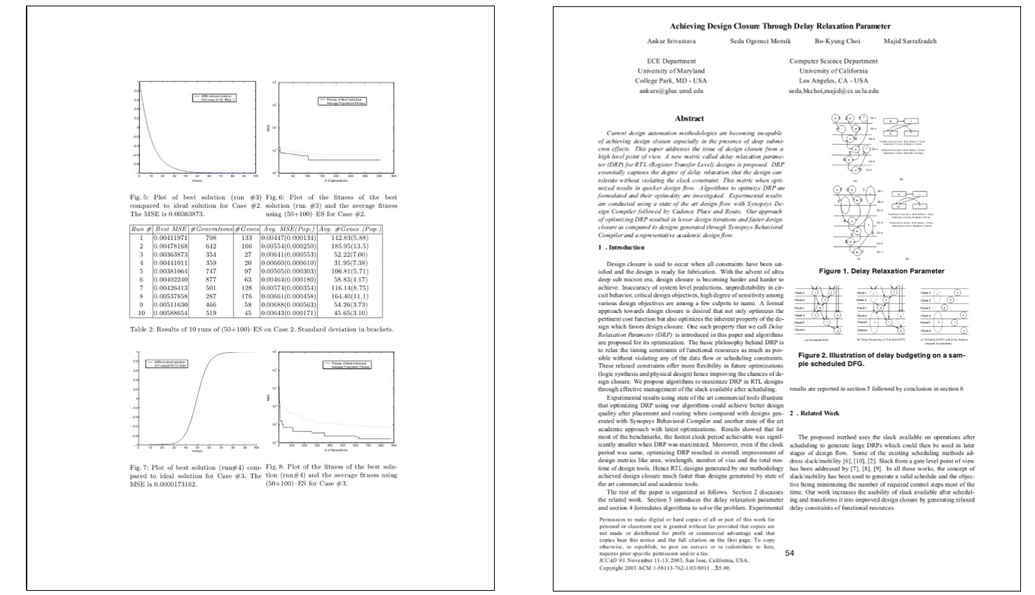
\includegraphics[width=1\columnwidth]{esempi_immagini_dataset_1} 
        \caption{Esempio di immagini presenti nel dataset}
        \label{img:example_dataset_images}
    \end{figure} 
    Per quanto riguarda il mio progetto ho preso in considerazione solamente le tabelle, ignorando le altre informazioni che si possono trovare. Dovendo infatti orientare la mia rete neurale ad analizzare polizze assicurative, ho preferito evitare di inserire elementi di disturbo - ad esempio, rilevazioni errate di oggetti non presenti - al fine di migliorare le \textit{detections}.
    \medskip
    \\Nel mio caso ho deciso di dedicare il $60\%$ del \textit{dataset} al \textit{training} e il $40\%$ al test. Purtroppo lo strumento offerto da \grayname{Tensorflow} non permetteva l'aggiunta della terza e molto importante parte della validazione, che serve per valutare l'affidabilità dei risultati ottenuti con la fase di test. Inoltre si può notare che ho dedicato molto spazio al test: il mio \textit{dataset} non è così grande, allora ho pensato di dedicare più immagini alla parte di test così da ridurre l'\gls{overfitting} nel quale altrimenti sarei potuto incappare.
    
    \subsection{Modifica delle immagini per migliorare l'apprendimento}
    Per allenare in maniera efficace la rete neurale bisogna ricordare il pre-allenamento eseguito dalle reti offerte da \grayname{Tensorflow}. Queste infatti sono allenate sui \textit{dataset}:
    \begin{itemize}
        \item COCO dataset\cite{site:coco-dataset};
        \item Kitti dataset\cite{site:kitti-dataset};
        \item Open Images dataset\cite{site:open-images-dataset};
        \item AVA v2.1 dataset\cite{site:ava-dataset};
    \end{itemize}
    Tutti questi \textit{dataset} trattano immagini a tre canali di colore e che contengono oggetti "uniformi", per così dire. \'E possibile immaginare quindi che la rete abbia imparato che c'è una sorta di "continuità" fra gli oggetti che poi sono identificati come tali. Al contrario, ho supposto che noi umani leggiamo le tabelle principalmente grazie ad una informazione spaziale: ovvero, sappiamo che la tabella è fatta così perché è composta da varie celle, possibilmente allineate. 
    \medskip
    \\Non essendo sicuro che questa informazione fosse facilmente recepibile dalla rete offerta da Google, ho cercato alcune soluzioni e mi sono imbattuto in un articolo scientifico, \textit{Table Detection using Deep Learning}\cite{article:table-detection-using-dl}. In questo articolo in particolare suggerivano di eseguire la seguente trasformazione\cite{site:distance-transform} sulle immagini con le tabelle:
    \begin{itemize}
        \item trasformazione euclidea della distanza sul canale blu;
        \item trasformazione lineare della distanza sul canale verde;
        \item trasformazione sul massimo della distanza sul canale rosso;
    \end{itemize}
    Per trasformazione della distanza si intende la rappresentazione della distanza tra il pixel a zero più vicino per ogni pixel dell'immagine.
    Il risultato di questa trasformazione si può apprezzare all'immagine \ref{img:distance-transformation}. Da notare che le immagini rispettano le proporzioni e le posizioni.
    \begin{figure}[H] 
        \centering
        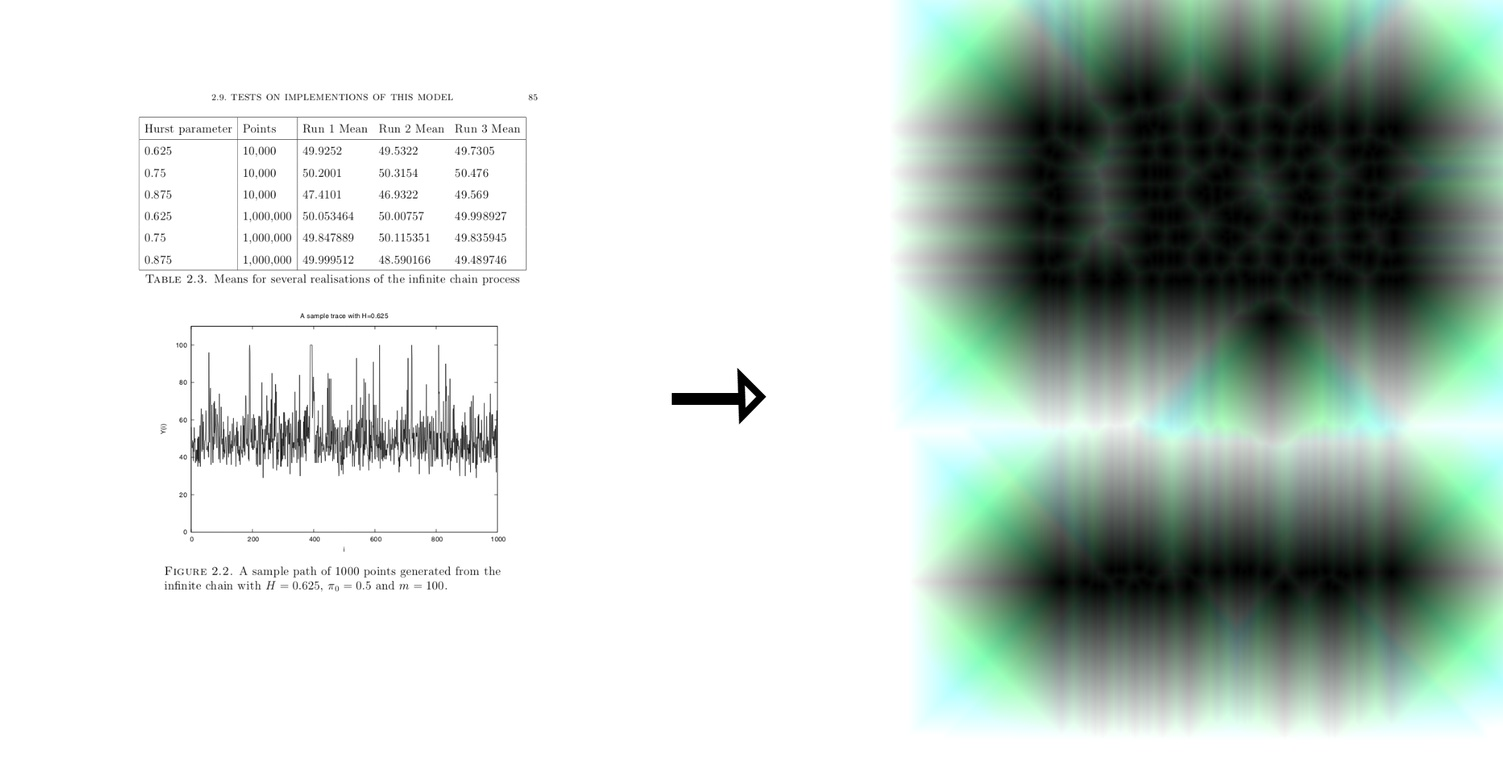
\includegraphics[width=1\columnwidth]{image-transformation} 
        \caption{Esempio di trasformazione dell'immagine con il calcolo delle distanze}
        \label{img:distance-transformation}
    \end{figure}
    Innanzitutto con questa trasformazione si possono annidare più informazioni - relative alle tre trasformazioni - su tre canali. Poi possiamo vedere come l'immagine assomigli di più ad una che la rete neurale pre-allenata si aspetterebbe: ovvero con una distribuzione semi omogenea di pixel, all'interno dei quali cercare le ricorrenze del caso. Possiamo infatti vedere come il grafico sia scarsamente rappresentato, poiché la quantità di pixel "colorati" è mediamente bassa. Lo è di più nella sua descrizione, ad esempio; inoltre intravediamo una certa organizzazione nella trasformazione della tabella: proprio quello che stavamo cercando!
    
    \subsection{Preparazione delle etichette}
    Le etichette del \textit{dataset} sul quale ho lavorato erano sotto forma di XML, uno per ogni immagine, all'interno del quale erano presenti le informazioni riguardandi le \textit{boxes} che racchiudono gli oggetti presenti nelle immagini. Poiché \grayname{Tensorflow} accetta solamente formati \grayname{pandas}\cite{prod:pandas} per le etichette, ho provveduto a trasformare le informazioni in due CSV distinti, uno per il training e l'altro per il test.
    
    \subsection{Creazione dei file \textit{TFRecord}}
    Creare i file \textit{TFRecord}, ovvero dei files di input che \grayname{Tensorflow} possa capire, avendo immagini ed etichette pronte, è abbastanza facile. \'E bastato infatti personalizzare lo script\cite{site:generate-tfrecord} offerto direttamente dall'API di Google.
    
    \subsection{Allenamento della rete neurale personalizzata}
    Come già anticipato è stato possibile non concentrarsi sul codice da scrivere per personalizzare la rete e riuscire a gestirla da un file di configurazione. I parametri - o, altresì chiamati nel gergo, \textit{hyperparameters} -, sono tanti e ognuno ha un'importanza maggiore o minore rispetto agli altri. Inoltre ho avuto la possibilità di scegliere da quale tipologia di architettura di rete neurale partire.
    \medskip
    \\L'allenamento è stato effettuato con la mia macchina, della quale caratteristiche scriverò brevemente:
    \begin{itemize}
        \item \textit{CPU}: Intel Core i5 8300H, 3.80GHz in Turbo Mode;
        \item \textit{GPU}: NVidia GTX1050 GDDR5 4GB RAM;
        \item \textit{RAM}: 8GB DDR4 2667MHz;
        \item \textit{Storage}: SSD NVMe 256GB
    \end{itemize}
        \subsubsection{Scelta della rete di partenza}
        Per quanto riguarda la scelta dei pesi iniziali, ovvero della rete neurale di partenza, non avendo molto tempo a disposizione ho deciso di effettuare una decisione a priori guardando le statistiche\cite{site:COCO-trained-model-statistics} degli allenamenti delle reti basati sul \textit{dataset} COCO\cite{site:coco-dataset}. La rete con risultati migliori a parità di velocità si è rivelata essere la \grayname{faster\textunderscore rcnn\textunderscore inception\textunderscore v2\textunderscore coco}, ho quindi basato tutti i miei successivi esperimenti su questa.
        \subsubsection{Scelta dei parametri da personalizzare}
        Per quanto invece concerne la scelta dei parametri, ho deciso di focalizzare la mia attenzione su alcuni di questi:
        \begin{itemize}
            \item \textit{image\textunderscore resizer}, che si occupa della dimensione e dei protocolli di ridimensionamento delle immagini;
            \item \textit{l2\textunderscore regulizer}, ovvero il peso della trasformazione L2\cite{site:l2-reg};
            \item \textit{first\textunderscore stage\textunderscore nms\textunderscore iou\textunderscore threshold} e \textit{iou\textunderscore threshold}, ovvero il peso dato all'IoU;
            \item \textit{optimizers} e \textit{learning\textunderscore rate}, ovvero la tipologia di \textit{optimizer}\cite{site:type_optimizers} utilizzato e come gestire il \textit{learning rate}.
        \end{itemize}
        Ho scelto di personalizzare solo questi principalmente per via della letteratura e dei corsi che ho seguito: questi infatti consigliavano di concentrarsi su questi parametri innanzitutto, poi di esplorare gli altri. Non avendo a disposizione molto tempo per testare ho quindi pensato di effettuare questa scelta.
        
        \subsubsection{Esempio di utilizzo di \grayname{Tensorboard}}
        \grayname{Tensorboard} è stato un valido alleato nell'allenare le reti neurali. Durante l'apprendimento permette di vedere l'andamento di due curve: una in arancione relativa al \textit{training}, una in blu relativa alla valutazione - che poi è quella più rilevante come "risultato". In particolare, i grafici che più ho tenuto sotto controllo sono stati:
        \begin{itemize}
%            \itemsep0em 
            \item la \textit{DetectionBoxes\textunderscore Precision/mAP (large)}, principalmente perché la maggior parte delle scatole da individuare corrispondevano a dimensioni generose, essendo le tabelle relativamente grandi rispetto all'immagine. Nell'immagine \ref{img:example_tensorboard_1} possiamo vedere la valutazione di una rete con \textit{adam optimizer};
            \item La \textit{loss}, per valutare se il \textit{training} o la valutazione stessero andando in \textit{overfitting}. Nell'immagine \ref{img:example_tensorboard_2} possiamo vedere l'andamento della perdita per una rete neurale con \textit{momentum optimizer}.
        \end{itemize}
        \begin{figure}[!h] 
            \centering
            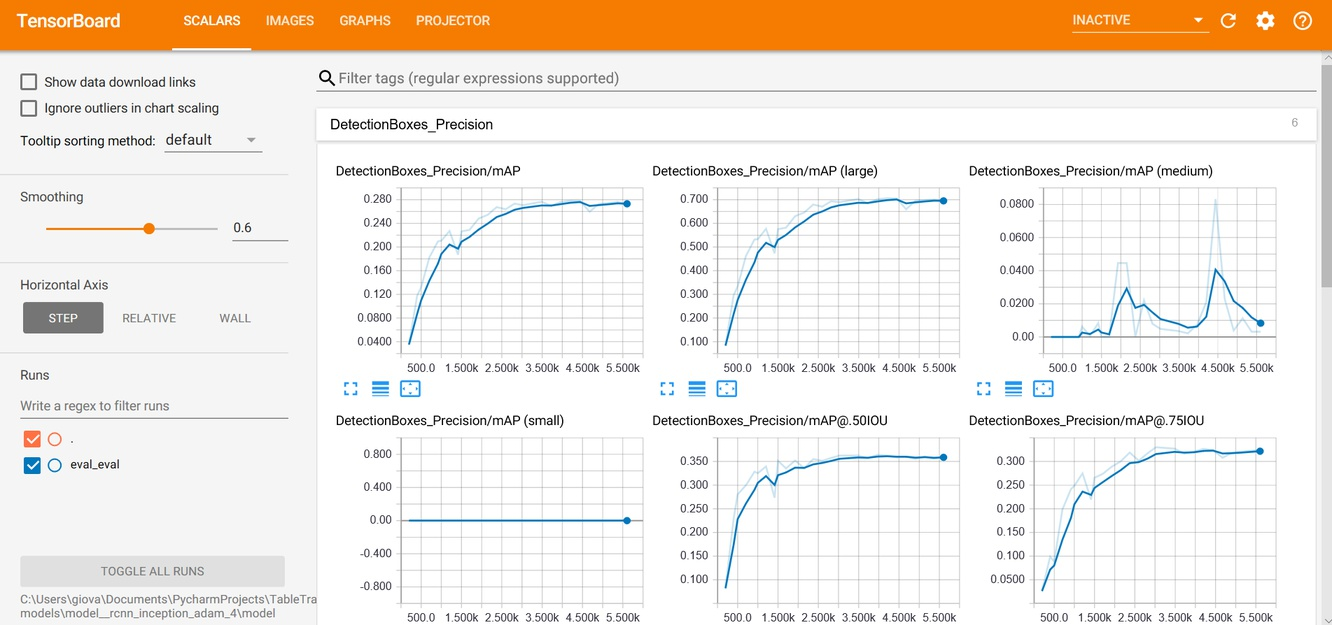
\includegraphics[width=1\columnwidth]{tensorboard-1} 
            \caption{Esempio di schermata classica con Tensorboard}
            \label{img:example_tensorboard_1}
        \end{figure}
        \begin{figure}[!h] 
        \centering
        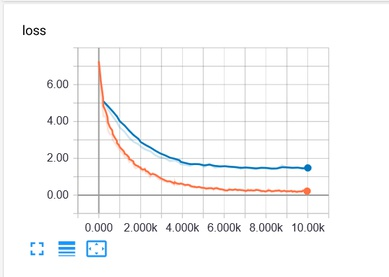
\includegraphics[width=0.7\columnwidth]{tensorboard-2} 
        \caption{Esempio di loss con \textit{Momentum Optimizer}}
        \label{img:example_tensorboard_2}
        \end{figure}
        
        \subsubsection{Considerazioni sui parametri}
        \paragraph{\textit{image\textunderscore resizer}}
        ~\\La personalizzazione di questo parametro è stata piuttosto semplice: ho dovuto trovare un buon compromesso tra grandezza dell'immagine da passare come input e la quantità di memoria a disposizione. Alla fine la scelta di ridimensionare in maniera fissa (quindi non rispettando le proporzioni dell'immagine) ogni immagine come input a $400x400px$ mi ha permesso una buona risoluzione a fronte di un'occupazione decente in RAM. Da notare che non rispettare le proporzioni dell'immagine - ovvero forzare una risoluzione predefinita - mi ha permesso di aumentare la \textit{batch\textunderscore size} oltre il valore predefinito di 1-
        \paragraph{\textit{l2\textunderscore regulizer}}
        ~\\L'impostazione di questo parametro è correlato alla presenza di \textit{overfitting} nel proprio modello. Grazie a \grayname{tensorboard} ho potuto tenere d'occhio l'andamento degli apprendimenti e, dopo molti tentativi, ho capito che probabilmente il valore che più si addice al mio \textit{dataset} è di $1*10^{-4}$ come valore iniziale, che poi aumenta fino a $4*10^{-4}$.
        \paragraph{\textit{first\textunderscore stage\textunderscore nms\textunderscore iou\textunderscore threshold} e \textit{iou\textunderscore threshold}}
        ~\\Questi due parametri gestiscono la metrica dell'IoU. Ho deciso di mettere mano anche a questo parametro dopo aver visionato il comportamento delle reti neurali quando testate (sezione \ref{sec:test-boxes}). Infatti mi sono reso conto che molto spesso la rete neurale confondeva una parte delle tabelle che avrebbe dovuto trovare per la tabella intera. Questo fatto è dovuto probabilmente alla diversità delle immagini del \textit{dataset} utilizzato per il training e di quelle che poi effettivamente sono presenti all'interno delle polizze. Un modo per mitigare questo effetto è stato quindi quello di abbassare il valore di questi due parametri a $0.5$.
        \paragraph{\textit{optimizers} e \textit{learning\textunderscore rate}}
        ~\\La scelta di questi due parametri è stata dettata dalla disponibilità dell'API di Google, dalla presenza di parametri di default e dalla letteratura. In particolare la disponibilità di \textit{optimizers} da parte dell'API è di:
        \begin{itemize}
            \item \textit{RMSPropOptimizer}\cite{site:RMSProp-optimizer};
            \item \textit{MomentumOptimizer}\cite{site:momentum-optimizer};
            \item \textit{AdamOptimizer}\cite{site:adam-optimizer}.
        \end{itemize}
        La scelta predefinita era impostata sul \textit{Momentum}. Tuttavia nei corsi seguiti su Coursera era emerso che l'\textit{Adam} avesse una migliore performance, a patto di regolare correttamente il \textit{learning rate}. Ho eseguito alcune prove con il \textit{momentum}, poi ho deciso di cambiare. Quindi, dopo aver impostato l'\textit{Adam} e il relativo \textit{learning rate} con la seguente formula (dell'\textit{exponentially decay learning rate}), dati $l_{r0}$ \textit{learning rate} iniziale, $t$ il numero di iterazioni e $k$ un parametro:
        \[l_r=l_{r0} * e^{(-k*t)}\]
        e dopo molte prove - per evitare un apprendimento troppo veloce oppure troppo lento -, sono arrivato ad impostare:
        \[l_{r0}=1exp^{-4}\]
        \[k=0.8\]
        \[decay\textunderscore steps=300\]
        dove \textit{decay\textunderscore steps} sono i passi dopo i quali valutare il nuovo \textit{learning rate}.
        
        \subsubsection{Interpretazione e modifica delle \textit{boxes}}
        \label{sec:interpretazione-modifica-boxes}
        La rete neurale è per lo più rimasta in allenamento per 7000 iterazioni per un tempo variabile tra le 4 e le 8 ore di tempo. Una volta esportato il grafo congelato, così da essere pronto per l'inferenza, ho potuto testare le varie configurazioni. In \ref{sec:test-boxes} troviamo i risultati visivi di quelle provate.
        \medskip
        \\Ci si rende subito conto di come l'identificazione delle tabelle non sia precisa. Soprattutto si nota come il più delle volte l'algoritmo confonde una parte per l'insieme, identificando solamente porzioni di tabella e spesso in maniera sovrapposta tra una identificazione e l'altra. Inoltre anche i punteggi non sono mai eccelsi: non appena si supera la valutazione di $0.8$ l'identificazione inizia ad essere lacunosa. 
        \medskip
        \\Ho quindi pensato ad una soluzione. Dal momento che conoscevo la tipologia di documenti che avrei dovuto analizzare, ho stilato le seguenti osservazioni:
        \begin{itemize}
            \item ogni tabella compare sempre senza testo attorno e a singola colonna;
            \item non ci sono mai più di quattro tabelle nella stessa pagina;
            \item le tabelle sono in formato misto, ma per lo più composto di parole e numeri.
        \end{itemize}
        Da queste informazioni ho dedotto di poter:
        \begin{itemize}
            \item tagliare la pagina non attorno alla scatola trovata ma su tutta la larghezza di quella. Così avrei diminuito l'errore dovuto all'individuazione, dovendo considerare solo due punti invece di quattro forniti (posizione di minimo e di massimo sull'asse verticale);
            \item unire le informazioni di alcune scatole con un punteggio abbastanza alto (personalmente impostato a $0.6$) che venivano tra loro sovrapposte, generando quindi un'unica grande \textit{box}.
        \end{itemize}
        Nella sezione \ref{sec:test-boxes} si potranno apprezzare le nuove scatole che, in rosso, individuano quindi la zona che si dovrà andare a tagliare.
    

\newpage
\section{IntelligentOCR}
    \subsection{\textit{Overview generale}}
    \grayname{IntelligentOCR} è l'effettivo programma che la mia azienda può utilizzare in maniera produttiva. Si occupa di distinguere le tabelle all'interno di documenti PDF - nel mio particolare caso, in polizze assicurative -, per poi poter processare in maniera diversa le une e il testo rimanente. Quindi, questo programma:
    \begin{enumerate}
        \item prende come input un file PDF e lo trasforma in immagini;
        \item per ogni immagine, ricerca tabelle al suo interno;
        \item processa ogni tabella con un estrattore di tabelle da documenti, così da restituirne la struttura e da restituirla su CSV;
        \item processa le immagini con testo puro al loro interno per estrarre del testo su TXT.
    \end{enumerate}
    Il focus durante la progettazione di questo programma è stato la leggibilità del codice e la leggerezza in RAM, poiché il programma è destinato a funzionare su un server con relativamente poca memoria a disposizione e ad essere manutenuto e migliorato da altre persone.
    
    \subsection{\textit{Design pattern} utilizzati}
    Tutti i passaggi di cui sopra mi hanno indotto a pensare ad una sorta di "catena di montaggio" per il mio prodotto, che lo rendesse facilmente migliorabile e testabile. Questo soprattutto in un'ottica aziendale: difficilmente mi occuperò di manutenere il prodotto che ho creato e un'altra persona dovrà riuscire a manutenerlo senza fatica.
    \medskip
    \\Essendo una sequenza di azioni non correlate fra loro ho pensato che il \textit{Pipeline Pattern}\cite{site:pipeline-pattern} potesse venirmi in aiuto. Infatti questo garantisce un'ottimo approccio per testare e per applicare il \textit{single responsibility principle}\cite{site:single-responsibility-principle}, in quanto ogni pezzo di codice fa solamente la sola o le due uniche cose per le quali è stato progettato, dopodiché passa il testimone al pezzo successivo. Non da meno, aumenta in maniera esponenziale la leggibilità del programma.
    \medskip
    \\Non da ultimo è da notare che è stato eseguito un approccio \textit{bottom-up}, ovvero dal basso verso l'alto. Ho cercato di costruire prima tutti i passaggi in maniera autonoma, senza che gli uni dipendessero dagli altri; ho poi provveduto alla composizione dei vari pezzi. Si può notare questo approccio nella composizione del file \textit{pipeline.py}, dove non vengono effettuate operazioni aggiuntive ma vengono solamente invocati i vari anelli della catena.
    
    \subsection{La \textit{pipeline}}
    Poiché il prodotto si configura proprio come una \textit{pipeline}, ne mostrerò la progettazione per parti. Si può apprezzare il fatto che ogni step è separato dagli altri in maniera stagna, tant'è che si può attivare l'output su disco oppure testare con documenti o immagini di prova in qualunque punto della catena di montaggio. 
        \subsubsection{Da PDF ad immagini}
        Un PDF è di per sé un formato prestante: può anche contenere delle informazioni relative al layout che poi possono essere utilizzate da lettori più o meno avanzati. Per questo motivo se un PDF non è frutto di una scansione, ma anzi è stato "stampato" digitalmente, allora tutto ciò che riguarda l'inferenza con rete neurali, la suddivisione in tabelle e testo, non ha più senso d'esistere perché esistono già molti strumenti che si occupano di interpretare tabelle.
        Tuttavia l'azienda mi ha esplicitamente chiesto di coprire il caso generale, ovvero di PDF provenienti da scansioni. In effetti si è poi capito che la stragrande maggioranza delle polizze assicurative presenti nel database era composto da PDF di siffatta natura.
            \paragraph{Estrazione}
            Ho quindi inizialmente provveduto all'utilizzo di \grayname{Wand}\cite{prod:wand}, \textit{wrapper} attorno a \grayname{ImageMagik}\cite{prod:imagemagik}, che esportava tutte le immagini in memoria, per poi poterle utilizzare nel resto della catena di montaggio. Tuttavia, dopo aver testato in maniera più approfondita il prodotto, mi sono reso conto che la memoria veniva occupata per centinaia di MB inutilmente, in quanto venivano caricate tutte le immagini del documento per poi comunque processarne una alla volta. Inoltre \grayname{ImageMagik} è affetto da un bug che, in caso di PDF di grandi dimensioni, fa sì che non liberi lo spazio temporaneo occupato su hard disk, portando all'occupazione di decine di GB inutilmente. Tutto ciò mi ha portato a cambiare approccio: innanzitutto ho proceduto all'utilizzo di \grayname{pdftoppm}\cite{prod:pdftoppm} da riga di comando direttamente da Python. Questo mi ha permesso di accedere una pagina alla volta ad ogni PDF, quindi di avere un'occupazione in RAM minima. Inoltre mi sono informato circa l'utilizzo dei \gls{generators} di Python, regolando quindi l'accesso ad ogni pagina solo quando effettivamente necessario.
            \medskip
            \\Da questo punto in poi tutti i passaggi vengono eseguiti su una pagina alla volta.
            \paragraph{Miglioramento dell'input}
            Una volta ottenuta la pagina possono essere eseguiti dei miglioramenti sull'input. In questo progetto viene solamente applicato un raddrizzamento attraverso \grayname{Alyn}\cite{prod:alyn}, ma è in questa sede che è possibile applicare altre trasformazioni. Una possibilità studiata ma non applicata in quanto non richiesto e per mancanza di tempo sarebbe stata la riduzione del rumore di fondo ispirandosi a dei \textit{kernels}\cite{site:denoysing-dirty-documents} offerti da Kaggle\cite{site:kaggle}.
        \subsubsection{Da immagini a ritagli}
        In questo stadio viene eseguita l'inferenza con la rete neurale descritta nella sezione \ref{sec:interpretazione-modifica-boxes}. Qui vengono replicati gli stessi passi: viene convertita l'immagine in un formato più "gradevole" per la rete neurale, vengono emesse le \textit{boxes} e vengono interpretate. A questo punto viene eseguito il taglio vero e proprio: si crea quindi una lista di immagini, in ognuna delle quali vengono memorizzate tutte le tabelle ritagliate dalla pagina originale, e un'immagine unica in cui vengono uniti tutti i ritagli rimanenti.
        \medskip
        \\A questo punto la lista di immagini e quella singola con tutto il testo vengono processate in maniera diversa.
        \subsubsection{Da tabelle a CSV}
        Ogni tabella della lista viene convertita ciascuna in un file PDF ricercabile con \grayname{Tesseract}\cite{prod:tesseract}. Questo è infatti l'unico formato che \grayname{Tabula}\cite{prod:tabula} accetta come input, per poter poi esportare la struttura calcolata.
        \subsubsection{Da immagini a testo puro}
        Ogni collage di immagini rimanenti dopo l'estrazione delle tabelle viene invece processato semplicemente da \grayname{Tesseract} e viene prodotto un file TXT con all'interno tutto il testo che lo strumento è riuscito a comprendere.
    \subsection{Risultati ottenuti}
    I risultati si possono visionare alla sezione \ref{sec:crop-polizze-assicurative}. Si può notare come non siano ancora ottimali. Come si può osservare alla sezione \ref{sec:good-test} nel caso di documenti ben formati il riconoscimento è sufficiente; tuttavia, se i documenti sono scansionati male, l'algoritmo funziona molto peggio (ad esempio in sezione \ref{sec:bad-test}). \'E tuttavia un passo in avanti notevole nella distinzione tra i due tipi di contenuti, sui quali poi si potranno eseguire altri tipi di analisi.
    
    
    
    
    
             % Kick-Off
% !TEX encoding = UTF-8
% !TEX TS-program = pdflatex
% !TEX root = ../tesi.tex
% !TeX spellcheck = it_IT

\chapter{Valutazione retrospettiva}
Si riporta di seguito una valutazione retrospettiva dell'esperienza di stage, al fine di valutare ciò che è stato fatto, le esperienze apprese e trarre insegnamenti per il futuro.

\section{Raggiungimento degli obiettivi}
Durante tutto il tempo di stage mi sono reso conto di dover continuamente tenere in considerazione le conoscenze da acquisire e la loro effettiva implementazione. La teoria da imparare è molta e non ho esaurito lo scibile in così poco tempo: ogni volta che mi si poneva un problema ho dovuto scegliere se risolverlo con un approccio teorico - e dispendioso in termini di tempo - oppure con uno funzionale, ma che non sempre permette di trarre insegnamenti validi. D'altro canto, il rischio opposto - ovvero di fossilizzarsi sulla teoria - era altrettanto pericoloso. Nonostante ciò ho raggiunto una buona copertura degli obiettivi definiti nel piano di lavoro.
\newpage
{
    \def\arraystretch{2}\tabcolsep=10pt
    \begin{table}[!ht]
        \small
        \begin{tabular}{ |p{1cm} |p{7cm}| p{3cm}|}
            \hline
            \textbf{ID} & \textbf{Descrizione} & \textbf{Stato} \\ \hline
            
            \multicolumn{3}{|c|}{\textbf{Obbligatori}} \\ \hline
            
            O01 & Creazione di un algoritmo che faciliti la creazione di un dataset per allenare una rete neurale & Completato \\ \hline
            O02 & Creazione di una struttura di testing per la valutazione visiva dei risultati ottenuti & Completato \\ \hline
            O03 & Creazione di un algoritmo di estrazione di informazioni mirate da un libretto assicurativo & Completato \\ \hline
            O04 & Gestione di tutti gli algoritmi il più automatica possibile, possibilmente tramite l'uso di costanti & Completato \\ \hline
            O05 & Utilizzo del linguaggio Python versione 3 & Completato \\ \hline
            
            \multicolumn{3}{|c|}{\textbf{Desiderabili}} \\ \hline
            
            D01 & Creazione di un batch multithreading per l'estrazione parallela di informazioni da più polizze & Completato \\ \hline
            
            \multicolumn{3}{|c|}{\textbf{Facoltativi}} \\ \hline
            
            F01 & Integrazione del sistema nell'infrastruttura dell'azienda & Non completato \\ \hline
            
        \end{tabular}
        \caption{Tabella raggiungimento degli obiettivi}
    \end{table}
}
\newpage
\section{Resoconto dell'analisi dei rischi}
Si riporta inoltre il riscontro dell'analisi dei rischi analizzati ad inizio stage.
{
    \def\arraystretch{2}\tabcolsep=10pt
    
    \begin{table}[H]
        \small
        \begin{tabular}{ |p{4.5cm} |p{2cm} |p{4.5cm}|}
            \hline
            \textbf{Descrizione} & \textbf{Verificato} & \textbf{Piano attuato} \\ \hline
            \textbf{Non conoscenza del linguaggio}: prima di iniziare lo stage non avevo mai programmato in Python; &
            SI & 
            Ho trovato dei meccanismi di apprendimento rapido del linguaggio, tramite corsi online e provando fin da subito a scrivere del codice per conto proprio. Inoltre ho chiesto spesso agli altri stagisti qualche domanda più tecnica che mi potesse risparmiare del tempo per la ricerca \\
            \hline
            
            \textbf{Non conoscenza della materia}: Prima dell'inizio dello stage la conoscenza teorica in mio possesso di \textit{machine learning}, \textit{deep learning} e di reti neurali era generale e per niente applicata &
            SI &
            Ho frequentato fin dalla prima settimana dei corsi specializzanti. \\ 
            \hline
            
            \textbf{Non conoscenza degli strumenti}: Per il \textit{machine learning} e il \textit{deep learning} esistono tutta una serie di strumenti già pronti all'uso che risparmiano molto tempo in fase di progettazione e codifica. &
            SI &
            Anche durante lo studio di preparazione ho avuto modo di confrontarmi con le tecnologie che poi sarei dovuto andare ad utilizzare \\
            \hline
            \textbf{Esami durante il lavoro}: Lo stage è iniziato senza avere la certezza di aver superato un esame, che avrei dovuto quindi sostenere durante il periodo di lavoro. &
            SI &
            Ho pianificato la progettazione in maniera tale per cui ho lasciato la fase di allenamento e test nel periodo subito antecedente l'esame. Così la sera sono riuscito a studiare proficuamente. \\
            \hline
        \end{tabular}
        \caption{Riscontro dell'analisi dei rischi}
    \end{table}
}
\section{Possibili miglioramenti futuri}
La scarsa conoscenza iniziale della teoria e degli strumenti non mi hanno permesso di ottimizzare al meglio il prodotto da me costruito. Sicuramente l'allenamento della rete neurale, fatto sulla macchina personale, è migliorabile. L'azienda dispone di uno spazio \glslink{aws}{AWS} che potrebbe essere sfruttato a questo scopo.
\medskip
\\C'è inoltre da segnalare la diversità dei \textit{dataset} di allenamento e di effettivo utilizzo: la creazione di un \textit{dataset} personalizzato è d'obbligo, in questo senso, per migliorare le prestazioni della rete. A questo scopo l'idea futura è quella di implementare l'algoritmo da me creato nella piattaforma, cosicché siano gli utenti stessi a correggere e generare il \textit{dataset} in maniera assistita.
\medskip
\\Altro punto da segnalare è modificare la \textit{pipeline} di inferenza in maniera tale che essa abbia la possibilità di evitare l'algoritmo di inferenza qualora il PDF sia riconosciuto come "stampato" e non scansionato da scanner.

\section{Conoscenze acquisite e valutazione finale}
Tra le conoscenze meramente tecniche ho avuto modo di acquisire un nuovo linguaggio di programmazione e moltissimi \textit{framework} che mi saranno estremamente utili nel percorso di studi magistrale e in prospettiva lavorativa. In particolare, l'aver imparato un po' della teoria che sta dietro i più famosi algoritmi di \textit{deep learning} e aver messo "le mani in pasta" per quanto riguarda \grayname{Tensorflow}, \grayname{OpenCV} e \grayname{Keras} ha centrato appieno le aspettative che avevo in mente ad inizio stage. Ho felicemente constatato che le capacità acquisite durante il corso di studi triennale mi hanno permesso di adattarmi perfettamente e senza troppe difficoltà alla mancata conoscenza di praticamente tutto ciò che riguardava lo stage.
\medskip
\\Non da meno ho imparato ad introdurmi in un team già preconfigurato dove il \textit{core} aziendale non è strettamente quello informatico, bensì quello assicurativo. In più ho potuto condividere moltissime curiosità, osservazioni e possibili sviluppi ulteriori riguardanti le reti neurali con un collega lavoratore presso RiskApp, Luca Bizzaro, che mi hanno stimolato enormemente per uno studio ulteriore, più approfondito e mirato dell'argomento.
\medskip
\\In conclusione l'esperienza presso RiskApp è stata estremamente proficua sotto entrambi gli aspetti umani e professionali e spero di poter ripete l'esperienza anche in futuro.



             % Conclusioni
\appendix                               
% !TEX encoding = UTF-8
% !TEX TS-program = pdflatex
% !TEX root = ../tesi.tex
% !TeX spellcheck = it_IT

\chapter{Appendice}
Qui di seguito sono presentati tutti gli allegati di cui si è discusso lungo il documento.
\section{\textit{Boxes} rilevate nei test}
\label{sec:test-boxes}
In questa sezione verranno mostrate le immagini di test con le scatole che la rete neurale ha trovato in essi. Per ogni test verranno presentate l'immagine originale e, a coppie, un'immagine con tutte le migliori scatole trovate sopra il punteggio di $0.6$ e la sua corrispondente con le scatole unite secondo l'algoritmo citato a \ref{sec:interpretazione-modifica-boxes}

\newpage
\subsection{Test 0}
\begin{figure}[!ht] 
    \centering
    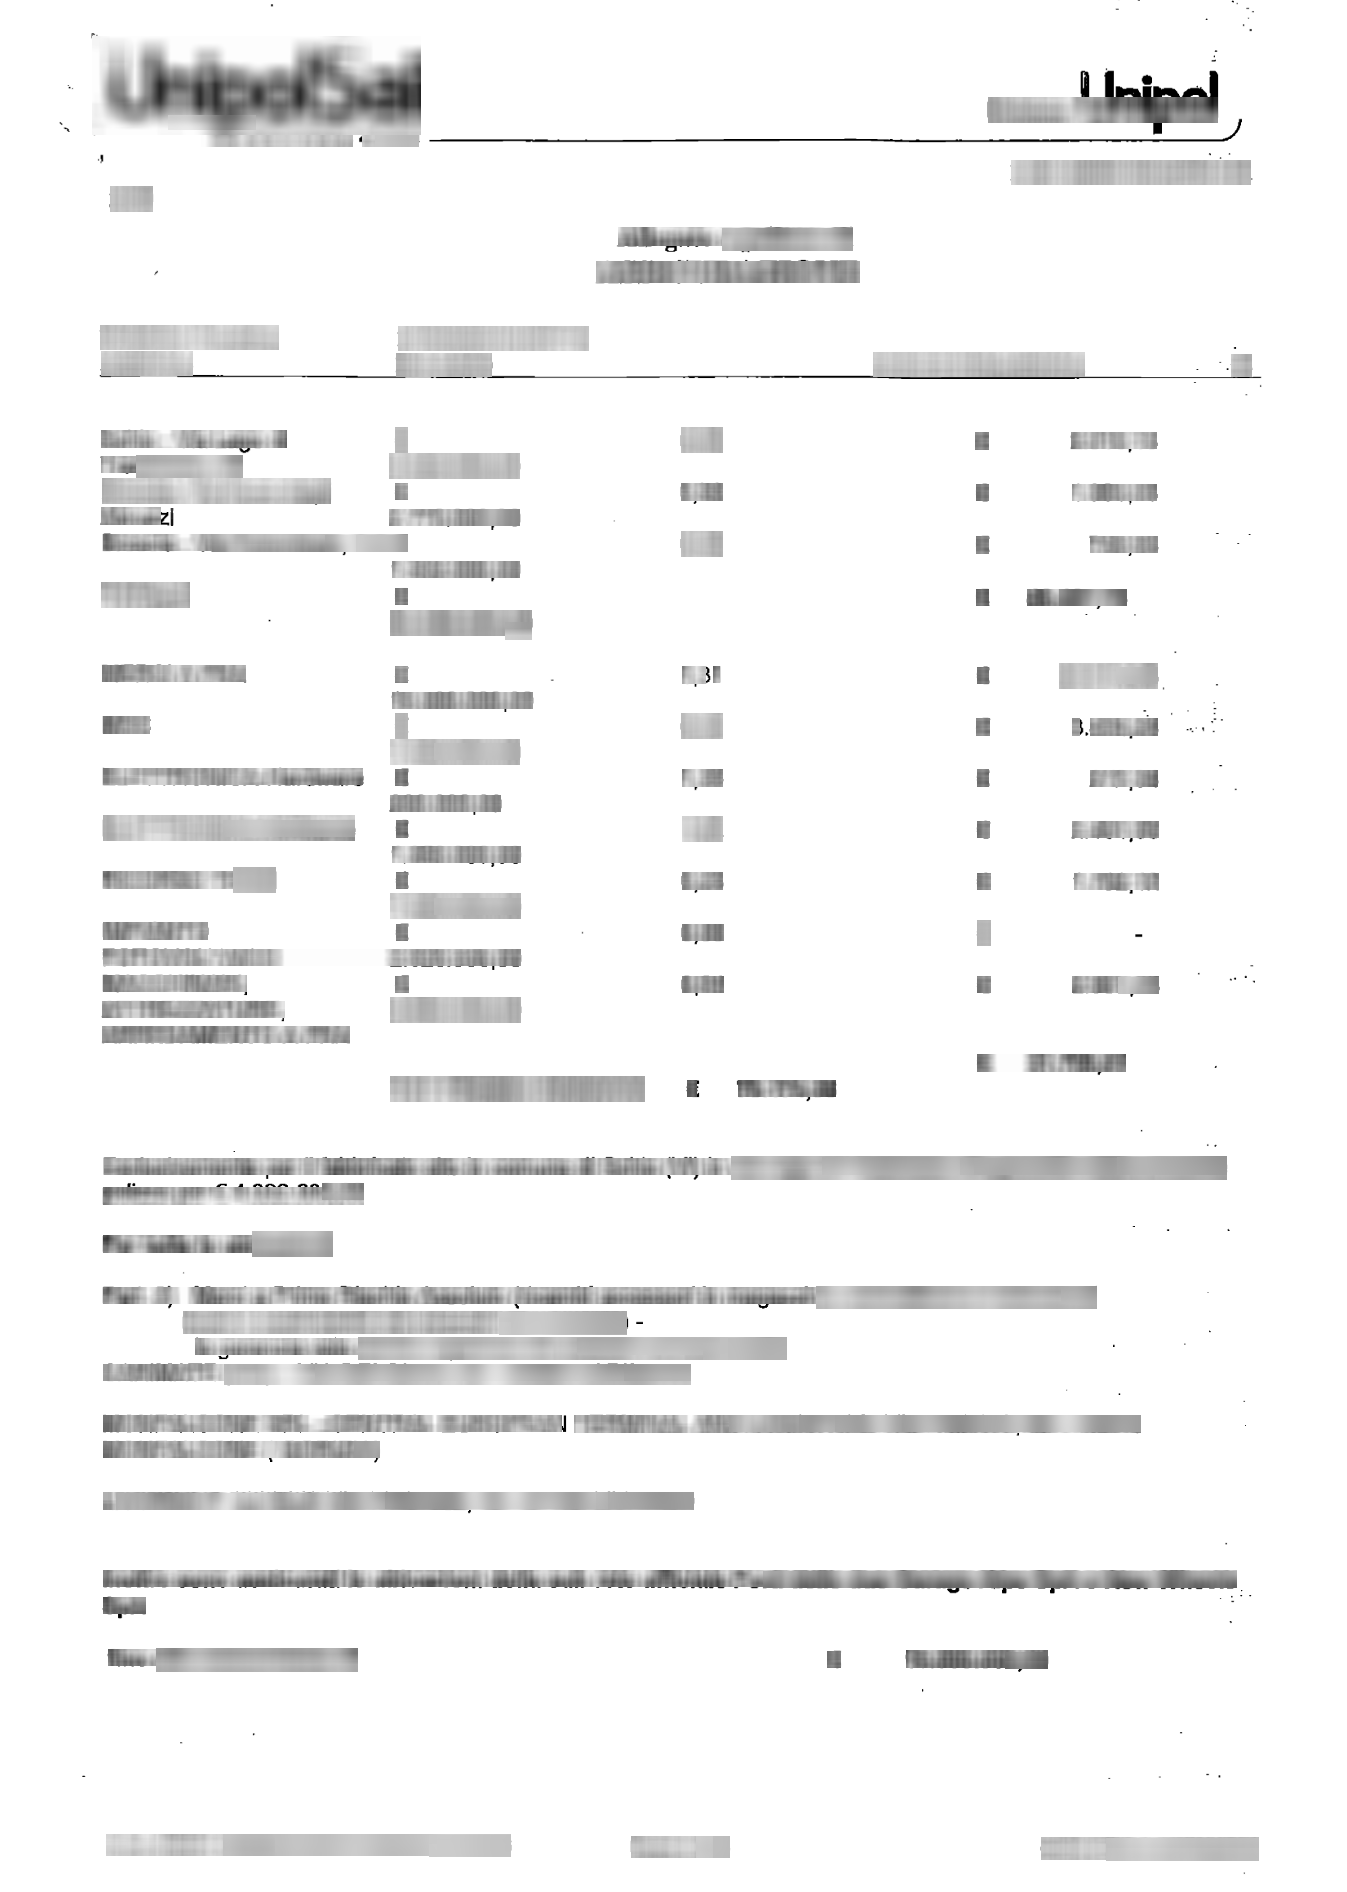
\includegraphics[width=1\columnwidth]{appendice/test0} 
    \caption{Test 0}
    \label{img:test-1}
\end{figure} 
\newpage

%============================================================================================


\begin{figure}[H]  
    \begin{minipage}{.5\columnwidth}  
        \centering  
        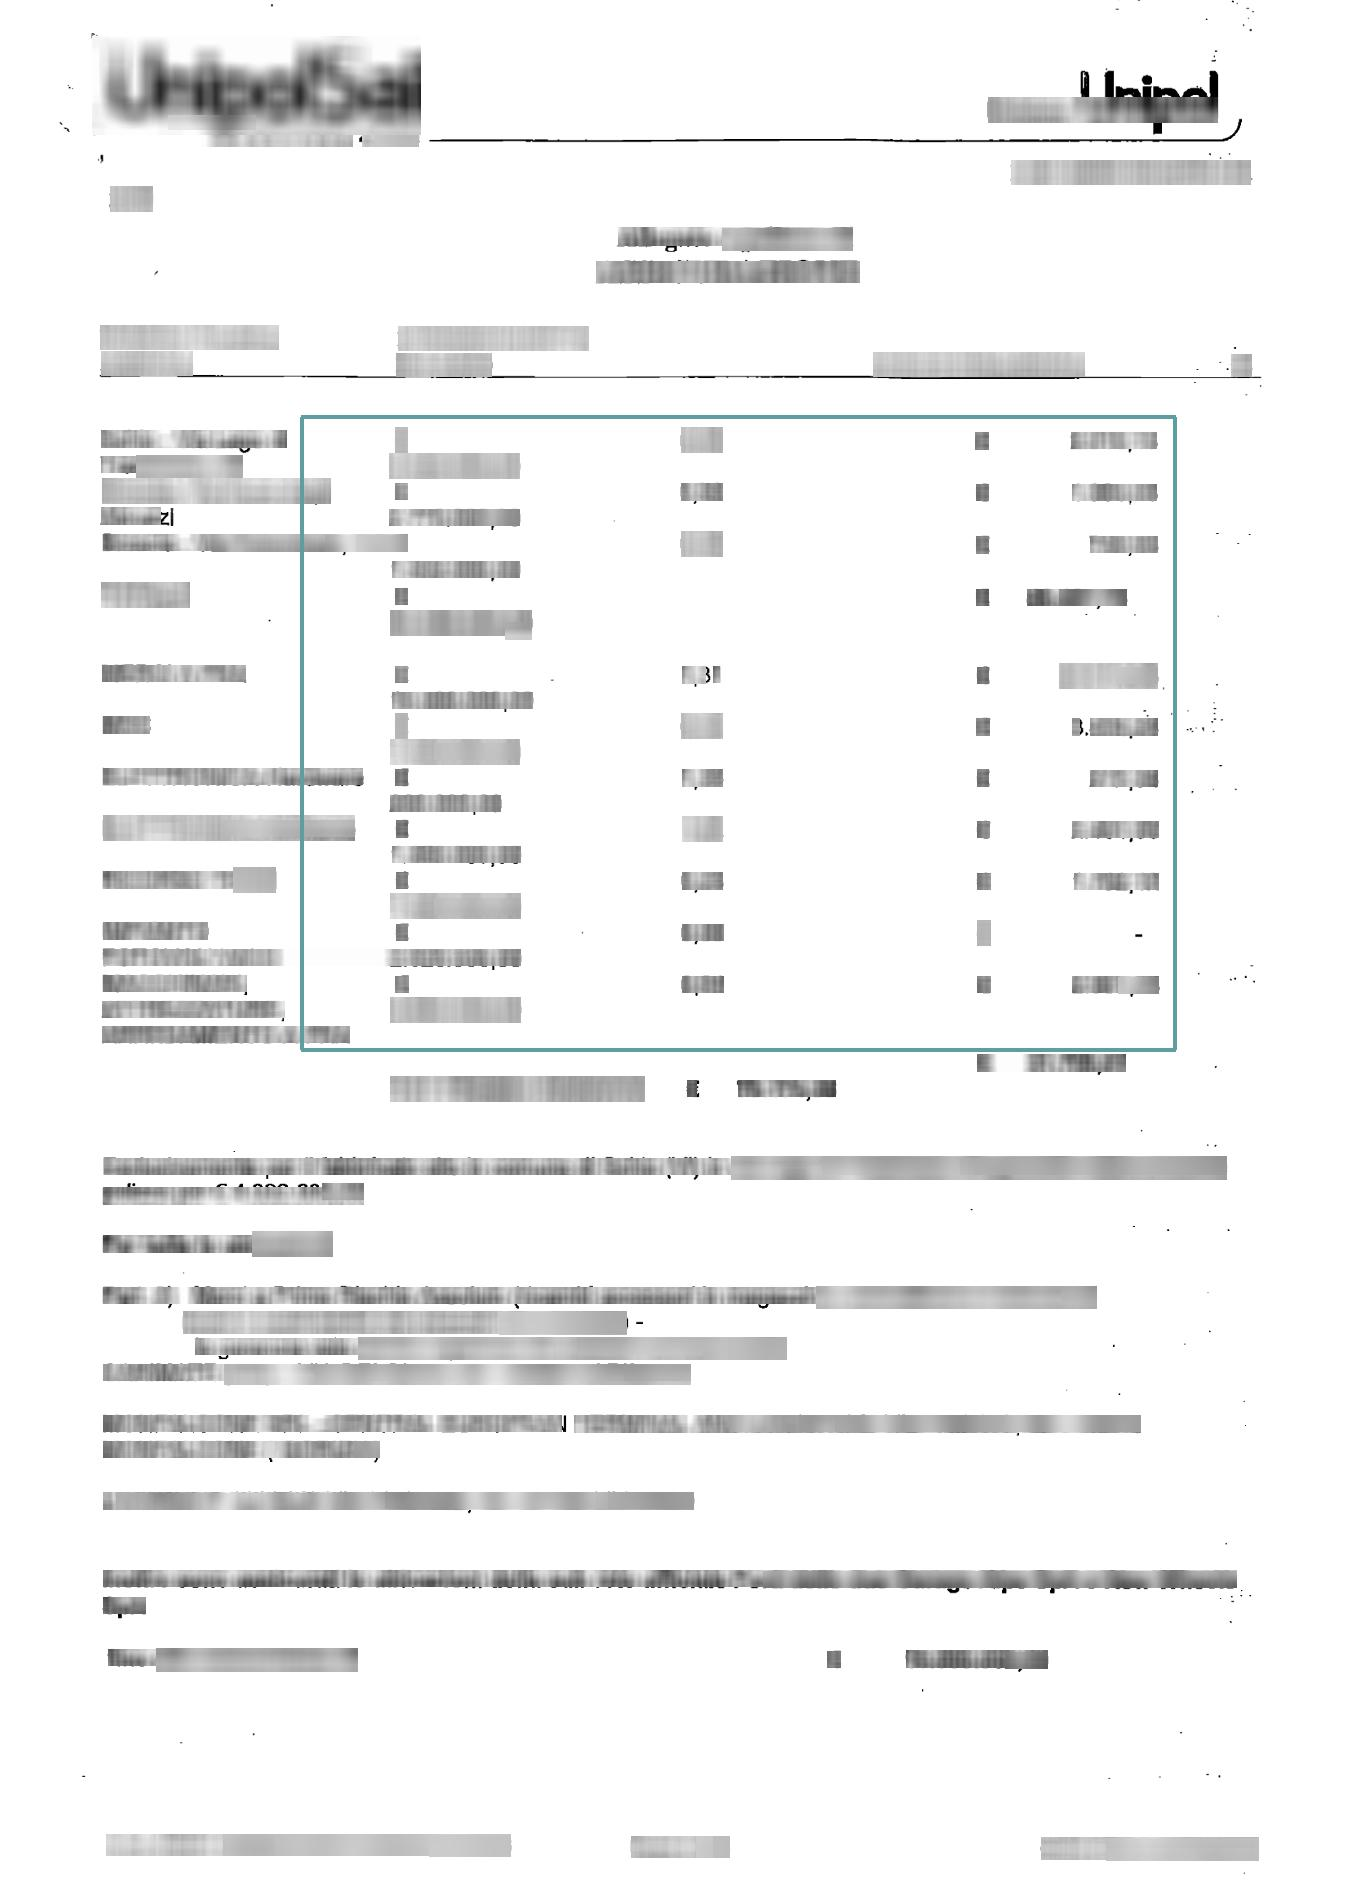
\includegraphics[width=1\columnwidth]{appendice/filtrate/test0_filtered_0_6_adam_1}  
    \end{minipage}%  
    \begin{minipage}{0.5\columnwidth}  
        \centering  
        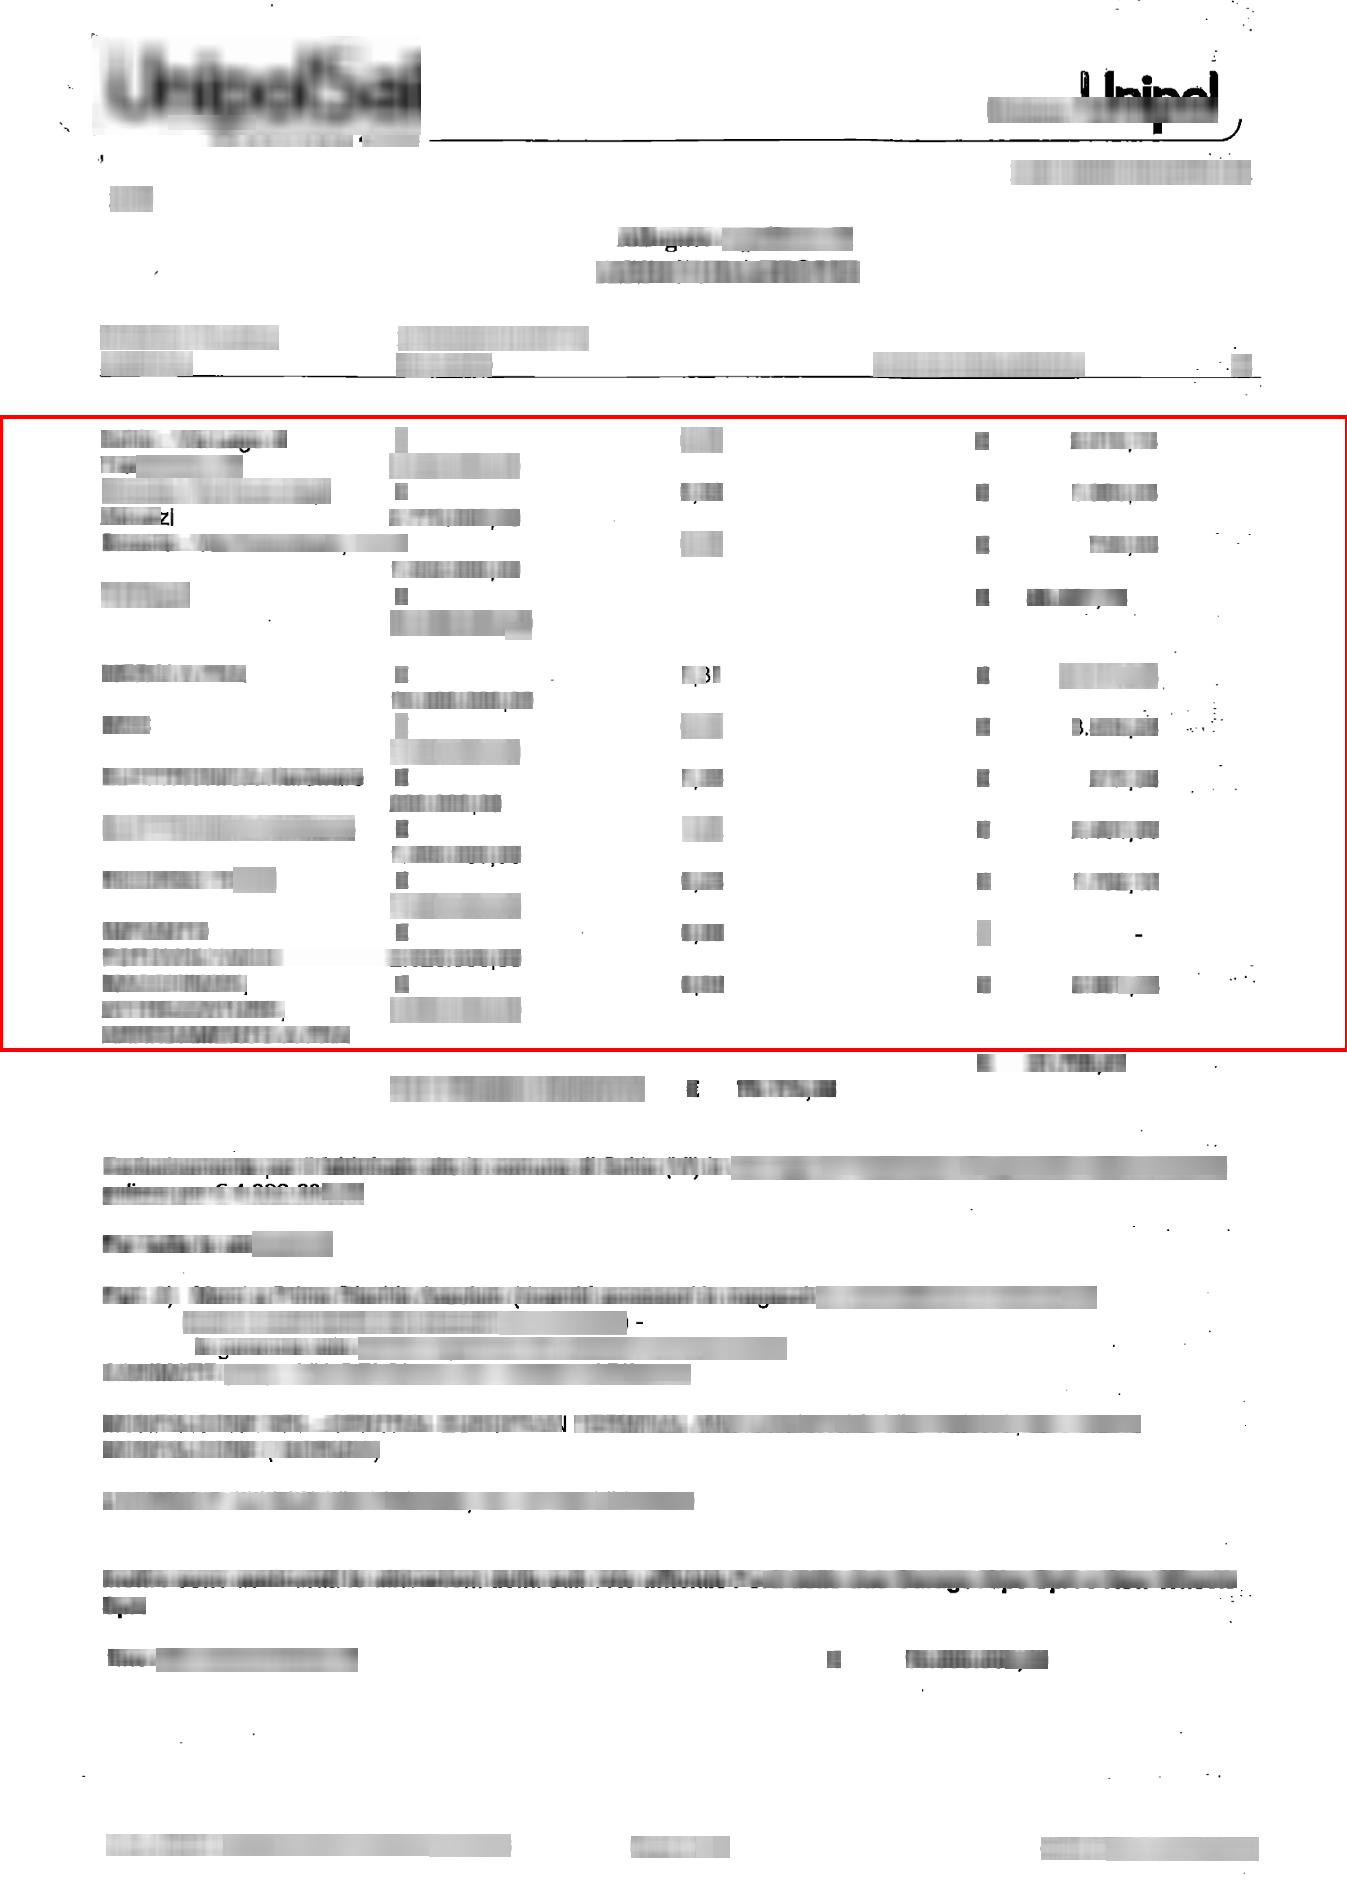
\includegraphics[width=1\columnwidth]{appendice/unite/test0_merged_0_6_adam_1}  
    \end{minipage}  
    \caption{Test 0, configurazione 1}
\end{figure}%  
Configurazione:
\begin{multicols}{2}
    \begin{lstlisting}
image_resizer {
  fixes_shape_resizer {
    width: 400
    heigth: 400
  }
}
first_stage_box_predictor {
  l2_regularizer {
    weight: 0.008
}
first_stage_nms_iou_threshold: 0.7
second_stage_box_predictor {
  l2_regularizer {
    weight: 0.004
  }
}
second_stage_post_processing {
  iou_threshold: 0.6
}
optimizer {
  adam_optimizer: {
    learning_rate: {
      manual_step_learning_rate {
        initial_learning_rate: .00008
        schedule {
          step: 4500
          learning_rate: .00004
        }
        schedule {
          step: 7000
          learning_rate: .00002
        }
        schedule {
          step: 10000
          learning_rate: .000008
        }
    ...
    }
    momentum_optimizer_value: 0.9
  }
  use_moving_average: false
}
\end{lstlisting}
\end{multicols}

%============================================================================================
\newpage
\begin{figure}[H]  
    \begin{minipage}{.5\columnwidth}  
        \centering  
        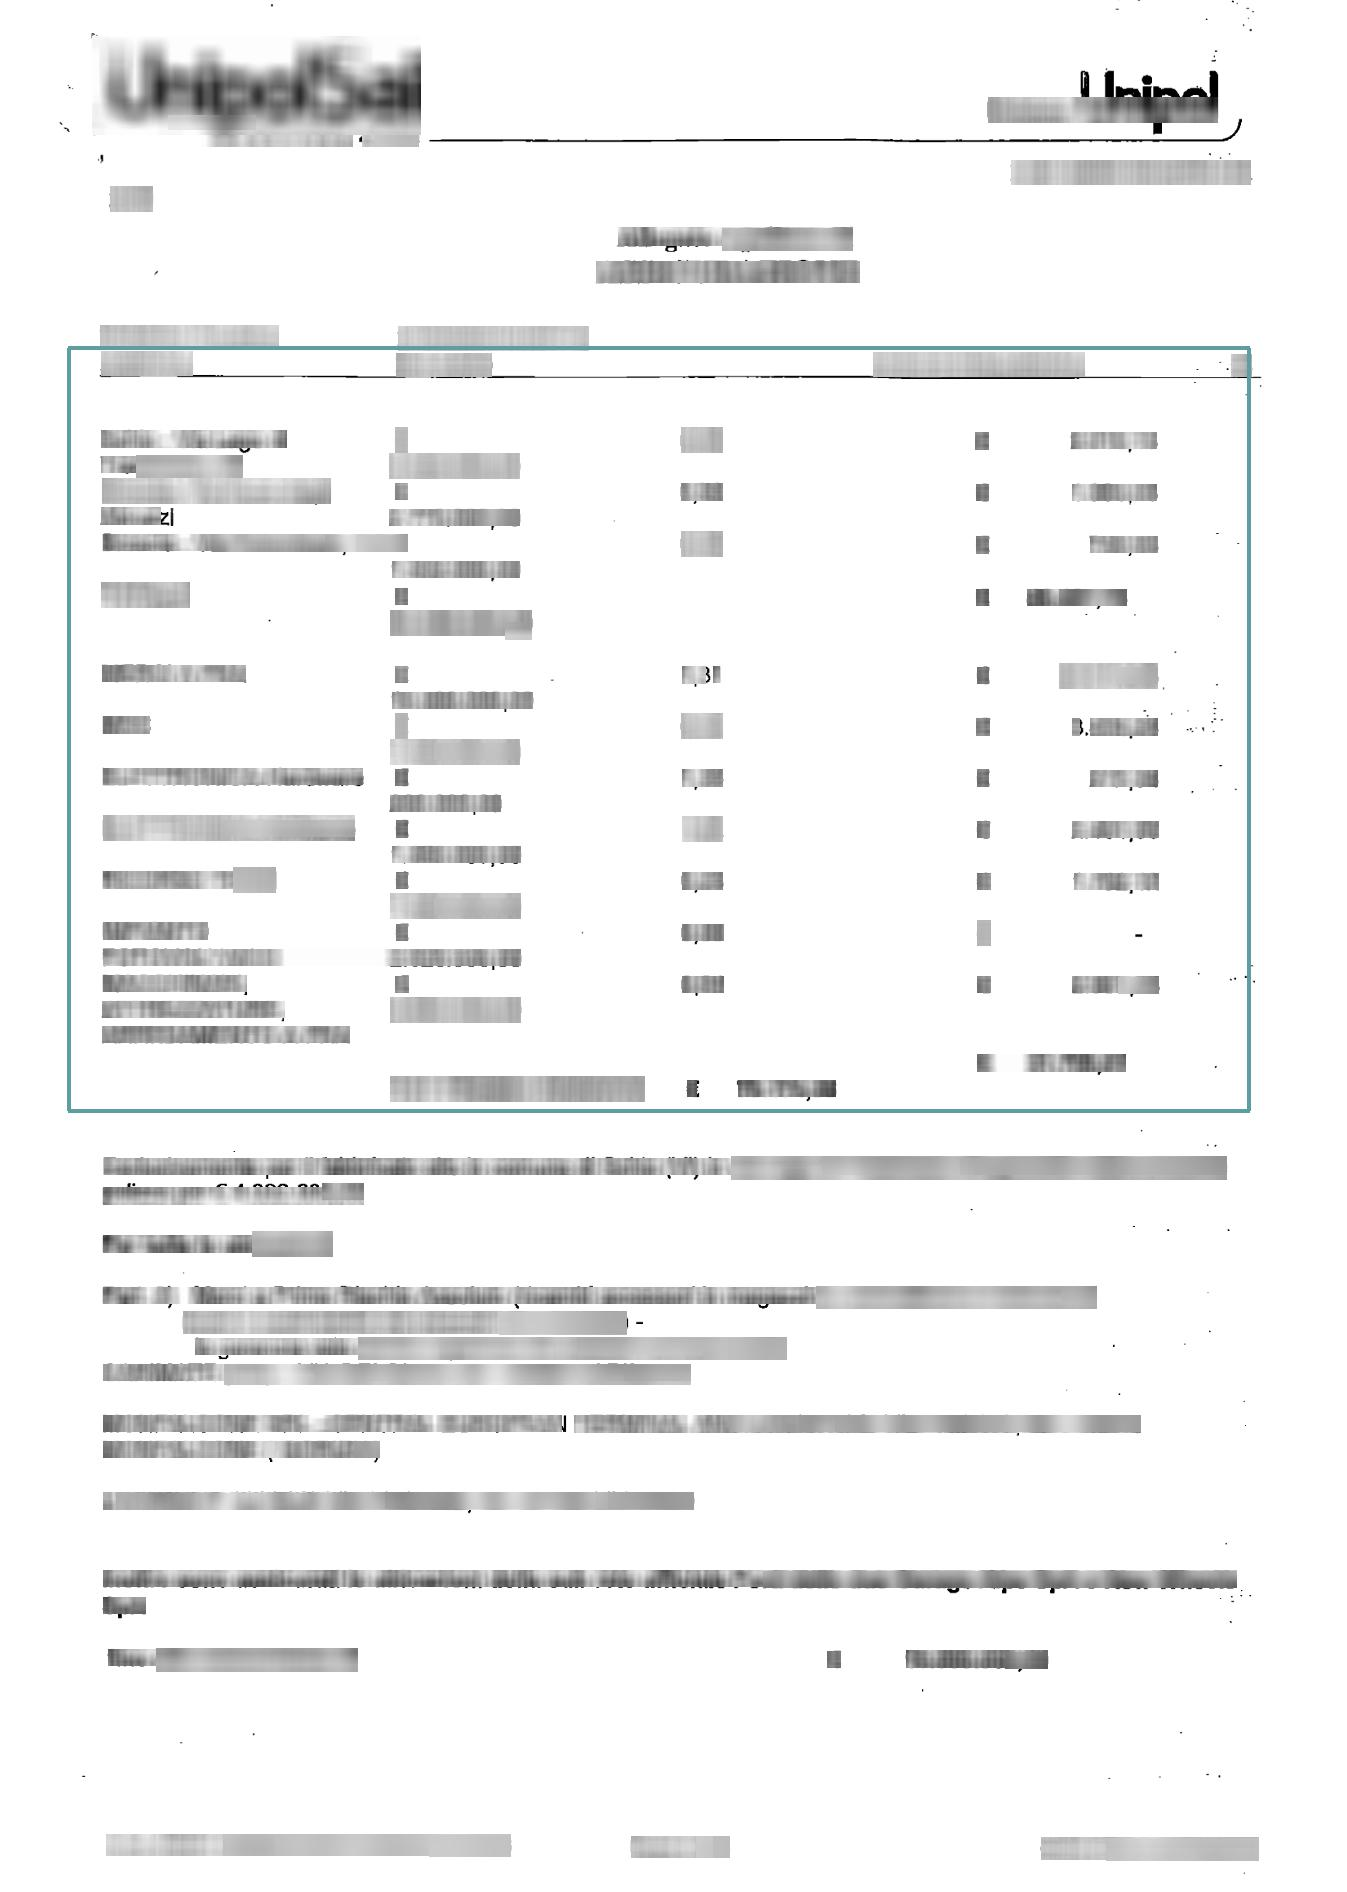
\includegraphics[width=1\columnwidth]{appendice/filtrate/test0_filtered_0_6_adam_3}  
    \end{minipage}%  
    \begin{minipage}{0.5\columnwidth}  
        \centering  
        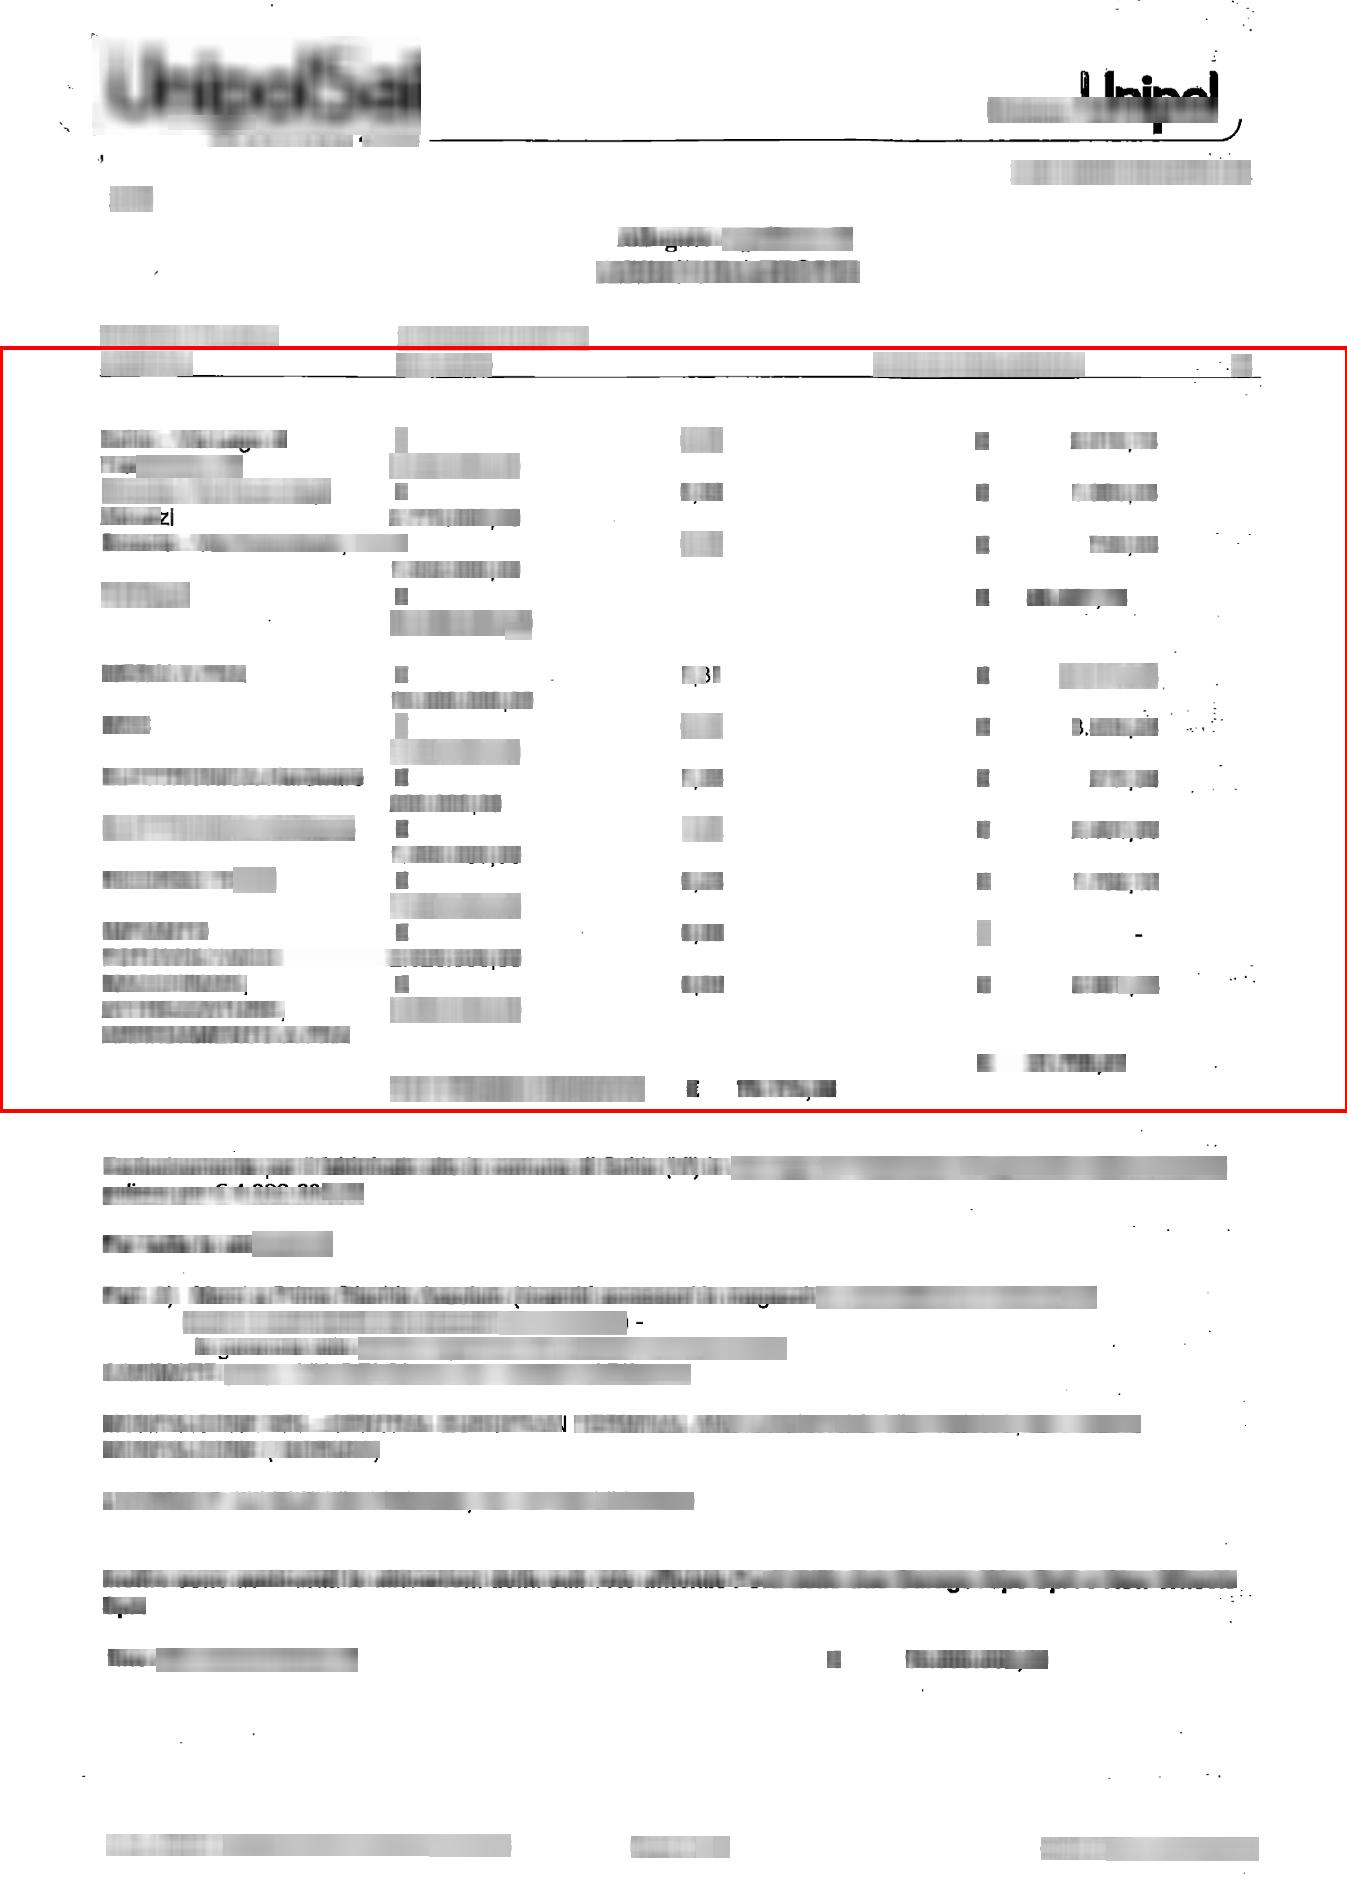
\includegraphics[width=1\columnwidth]{appendice/unite/test0_merged_0_6_adam_3}  
    \end{minipage}  
    \caption{Test 0, configurazione 2}
\end{figure}%  
Configurazione:
\begin{multicols}{2}
    \begin{lstlisting}
image_resizer {
  fixes_shape_resizer {
    width: 400
    heigth: 400
  }
}
first_stage_box_predictor {
  l2_regularizer {
    weight: 0.00001
}
first_stage_nms_iou_threshold: 0.7
second_stage_box_predictor {
  l2_regularizer {
    weight: 0.00004
  }
}
second_stage_post_processing {
  iou_threshold: 0.6
}
optimizer {
  adam_optimizer: {
    learning_rate: {
      exponential_decay_learning_rate {
        initial_learning_rate: 0.0001
          decay_steps: 600
          decay_factor: 0.95
        }
      }
    ...
  use_moving_average: false
}
    \end{lstlisting}
\end{multicols}

%============================================================================================
\newpage
\begin{figure}[H]  
    \begin{minipage}{.5\columnwidth}  
        \centering  
        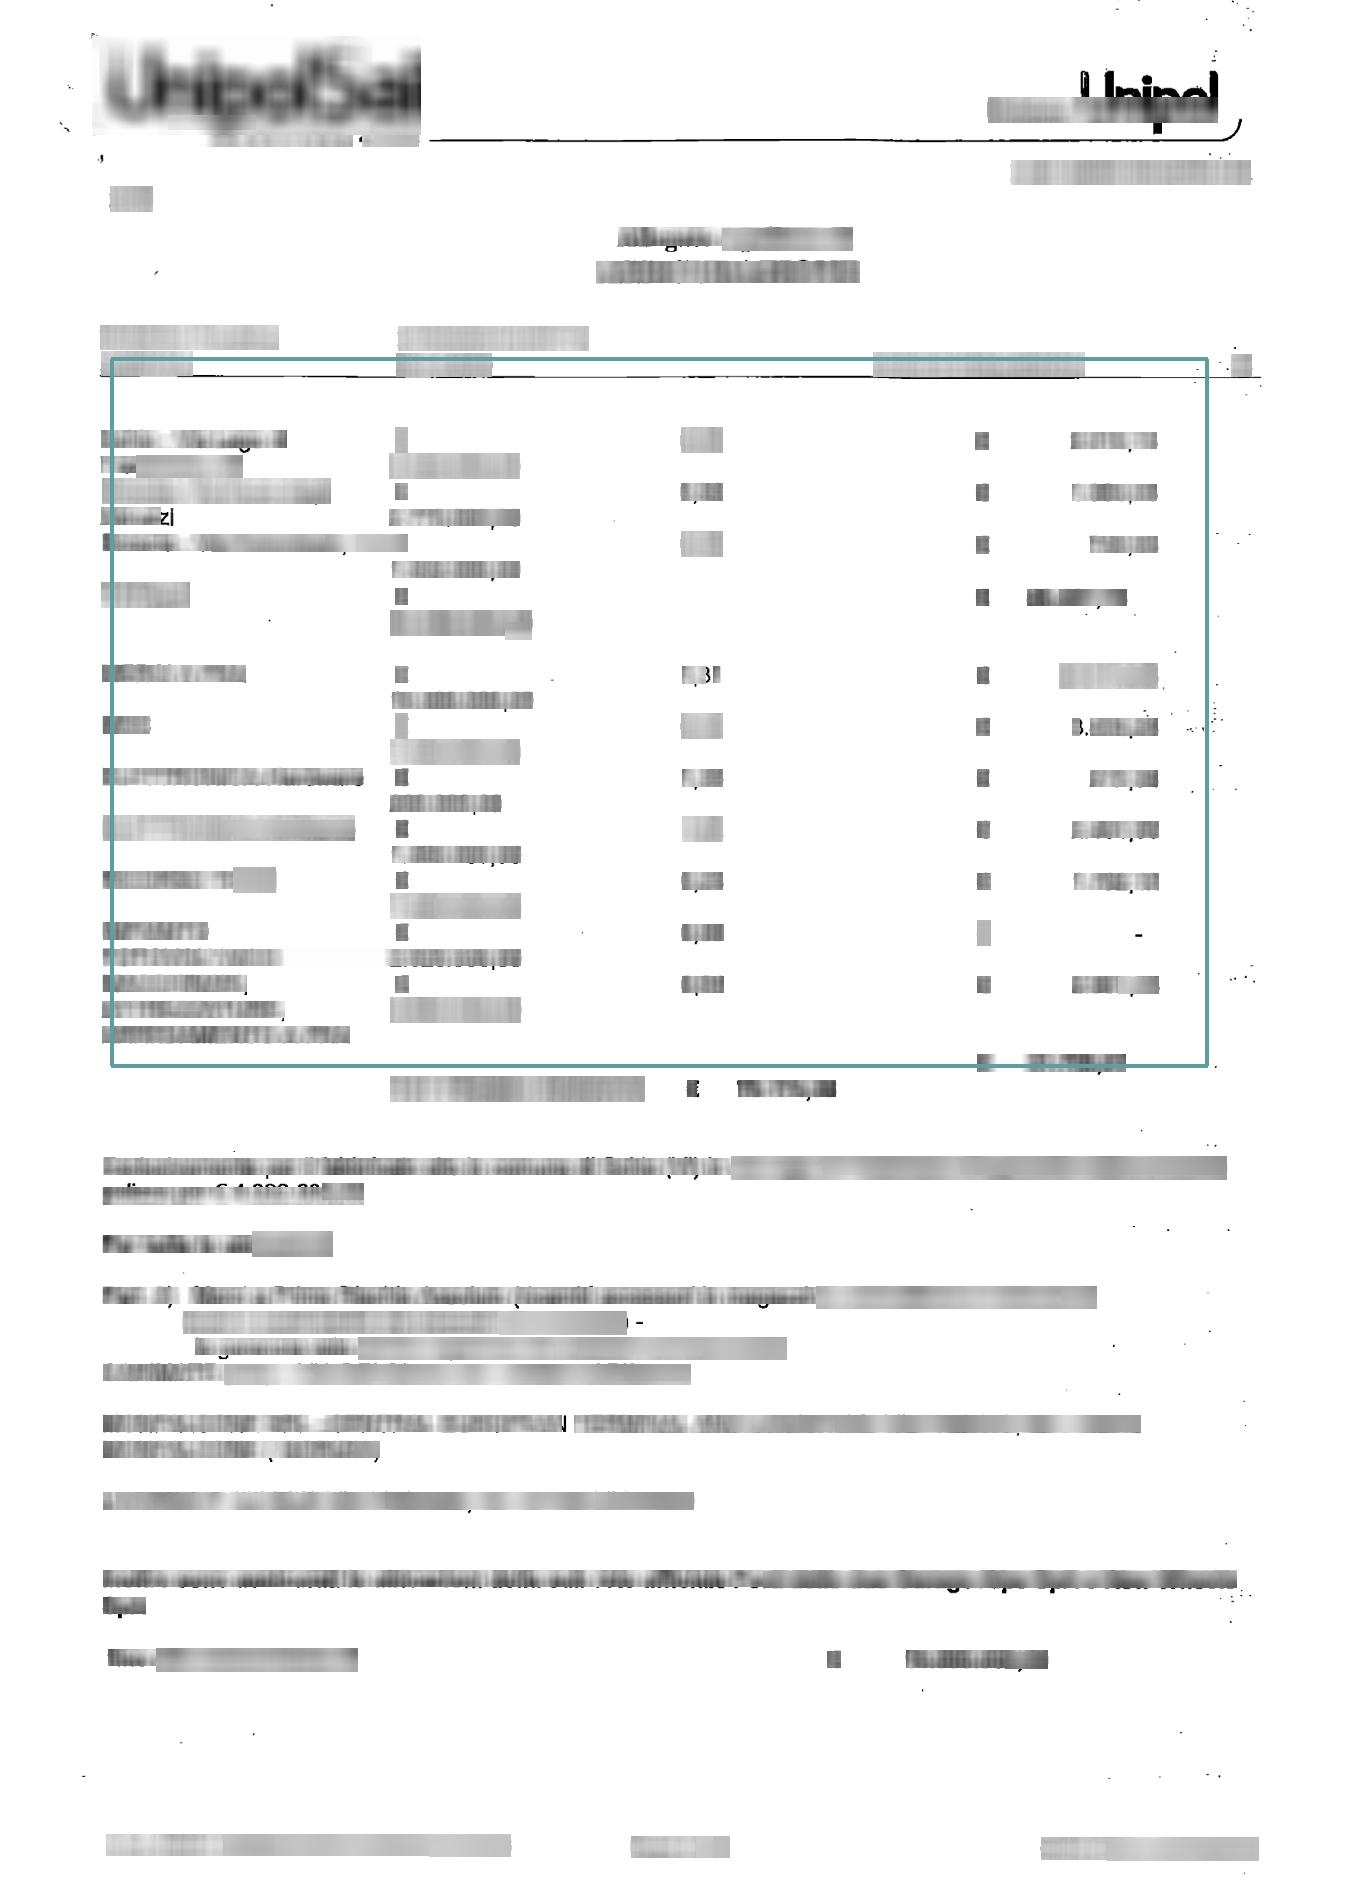
\includegraphics[width=1\columnwidth]{appendice/filtrate/test0_filtered_0_6_adam_4}  
    \end{minipage}%  
    \begin{minipage}{0.5\columnwidth}  
        \centering  
        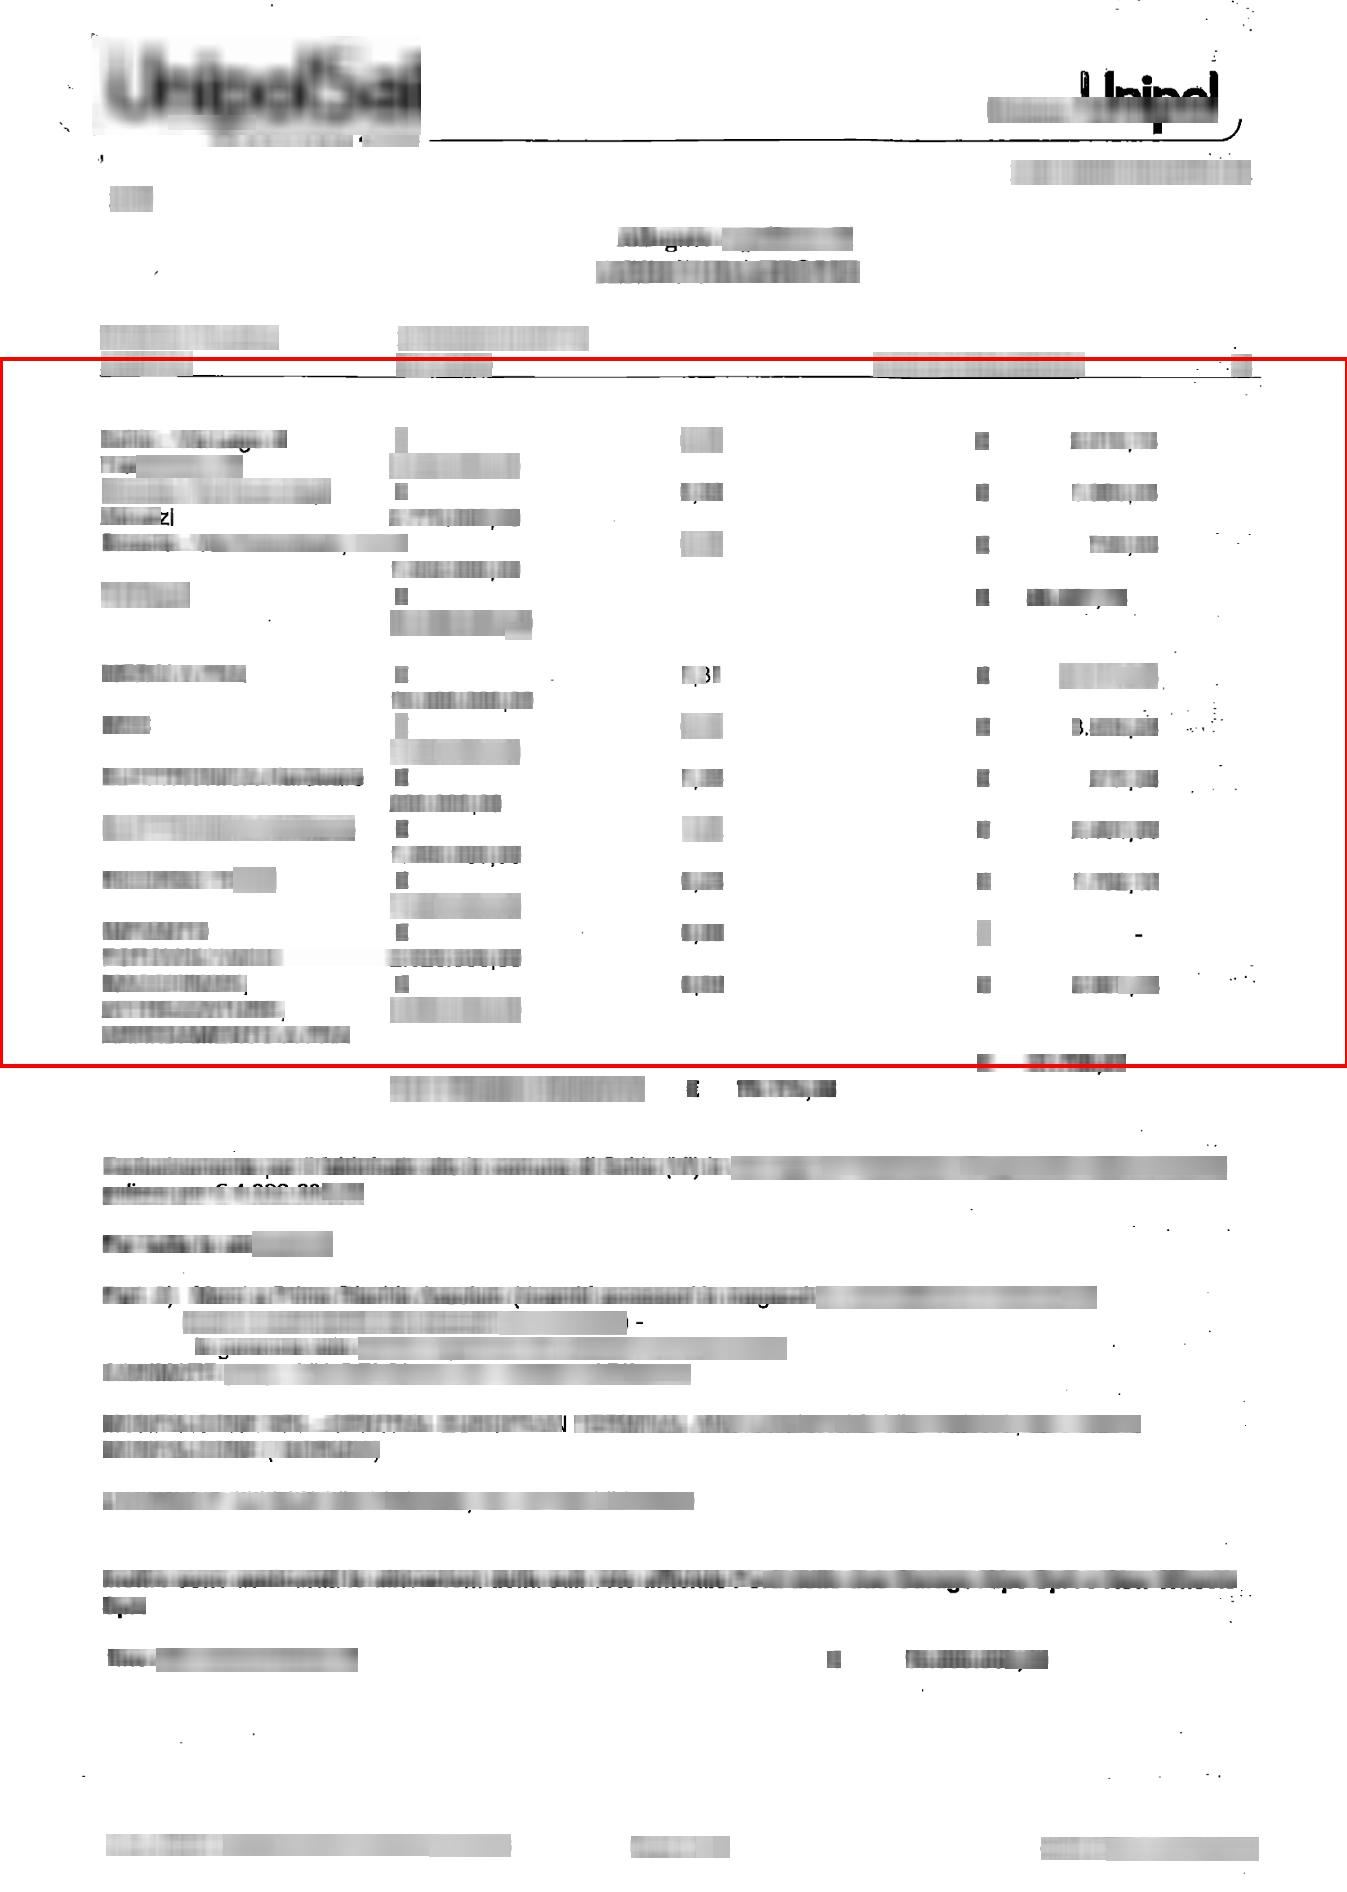
\includegraphics[width=1\columnwidth]{appendice/unite/test0_merged_0_6_adam_4}  
    \end{minipage}  
    \caption{Test 0, configurazione 3}
\end{figure}%  
Configurazione:
\begin{multicols}{2}
    \begin{lstlisting}
image_resizer {
  fixes_shape_resizer {
    width: 400
    heigth: 400
  }
}
first_stage_box_predictor {
  l2_regularizer {
    weight: 0.04
}
first_stage_nms_iou_threshold: 0.7
second_stage_box_predictor {
  l2_regularizer {
    weight: 0.004
  }
}
second_stage_post_processing {
  iou_threshold: 0.6
}
optimizer {
  adam_optimizer: {
    learning_rate: {
      exponential_decay_learning_rate {
        initial_learning_rate: 0.0001
          decay_steps: 450
          decay_factor: 0.9
        }
      }
    ...
  use_moving_average: false
}
    \end{lstlisting}
\end{multicols}

%============================================================================================
\newpage
\begin{figure}[H]  
    \begin{minipage}{.5\columnwidth}  
        \centering  
        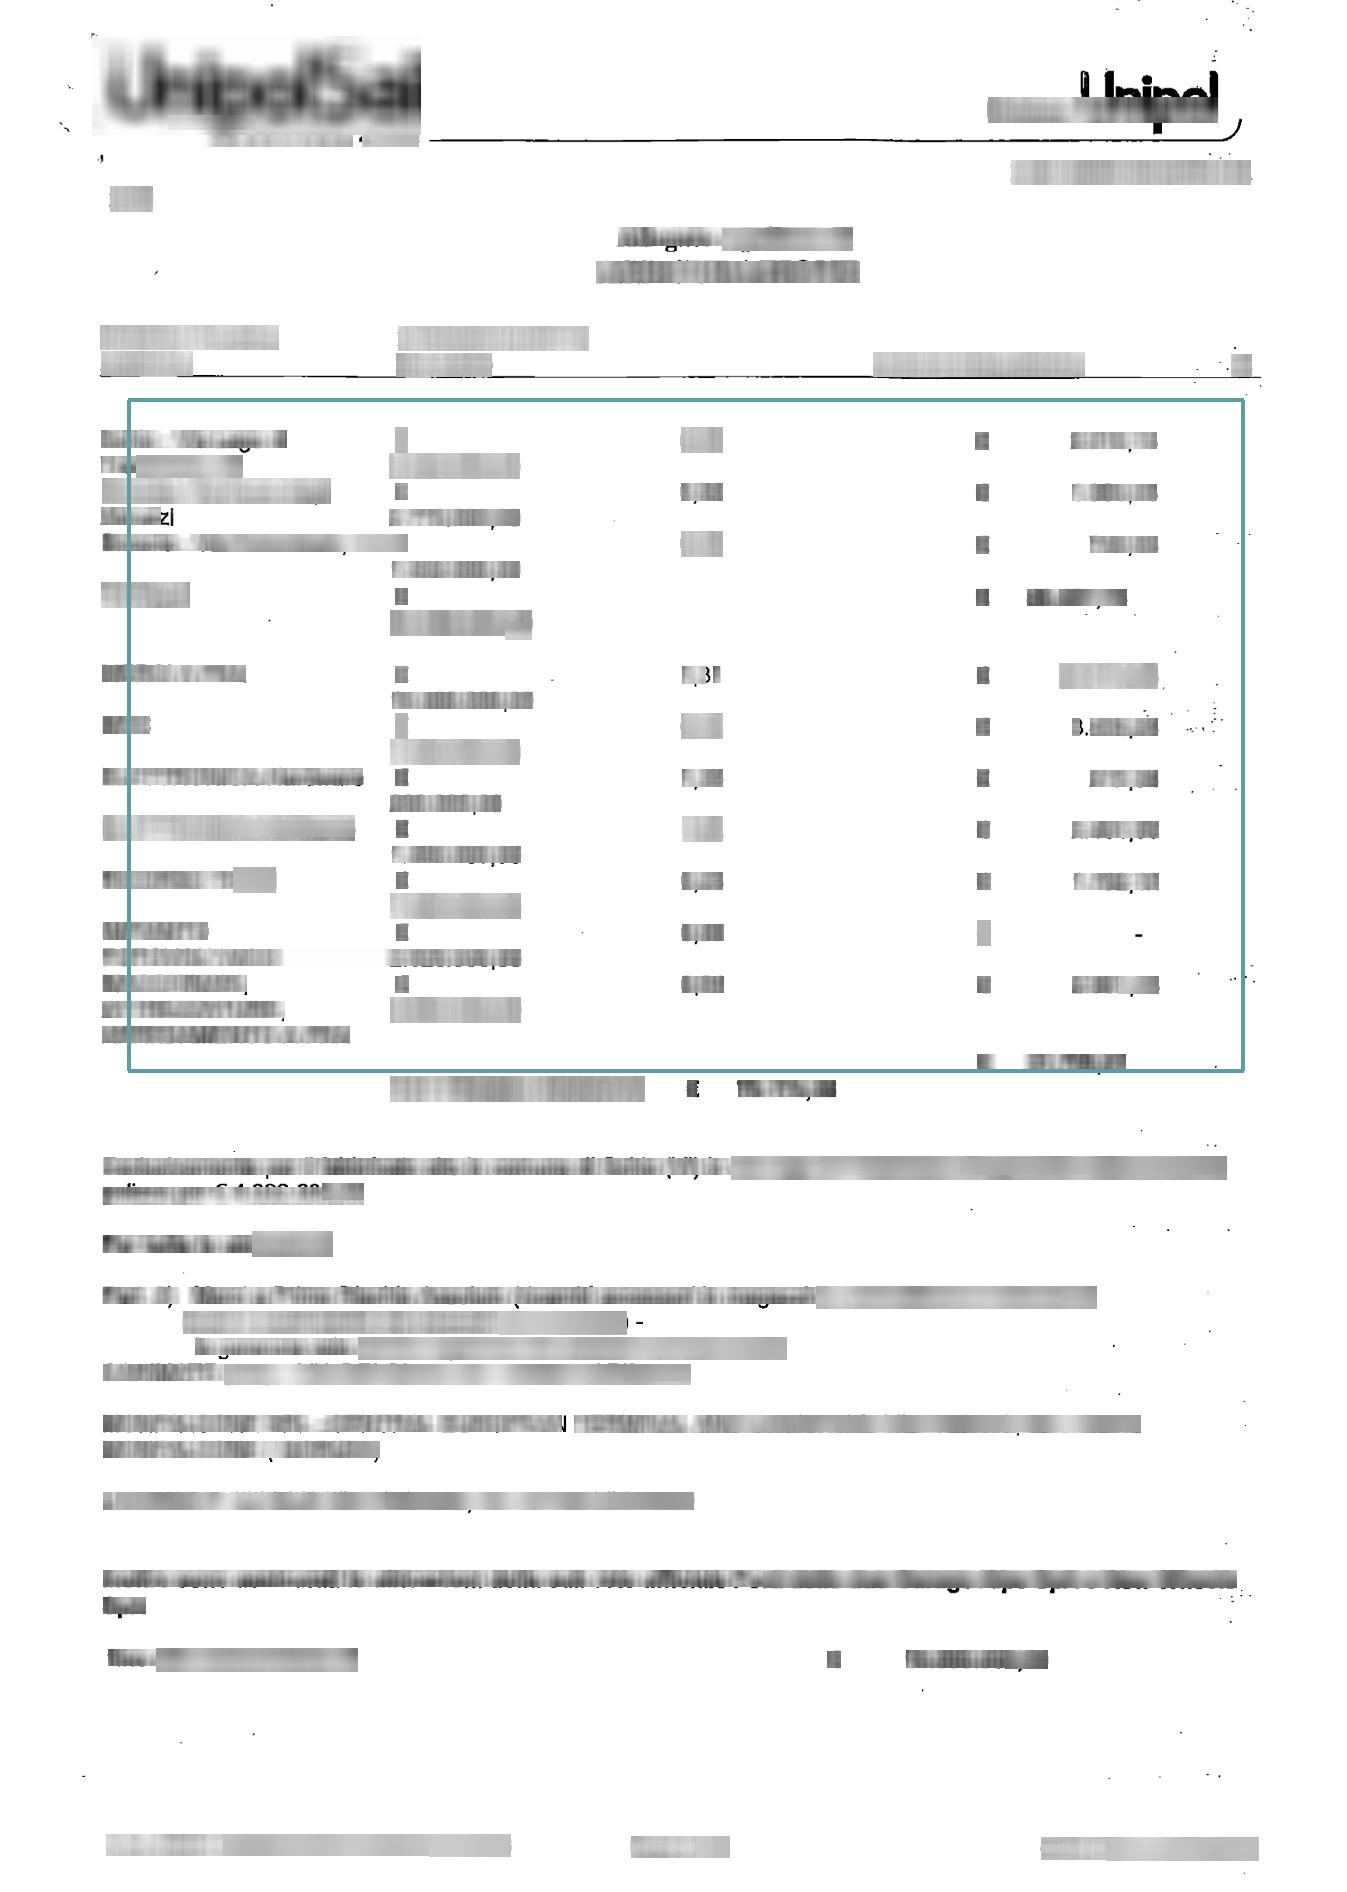
\includegraphics[width=1\columnwidth]{appendice/filtrate/test0_filtered_0_6_momentum_1}  
    \end{minipage}%  
    \begin{minipage}{0.5\columnwidth}  
        \centering  
        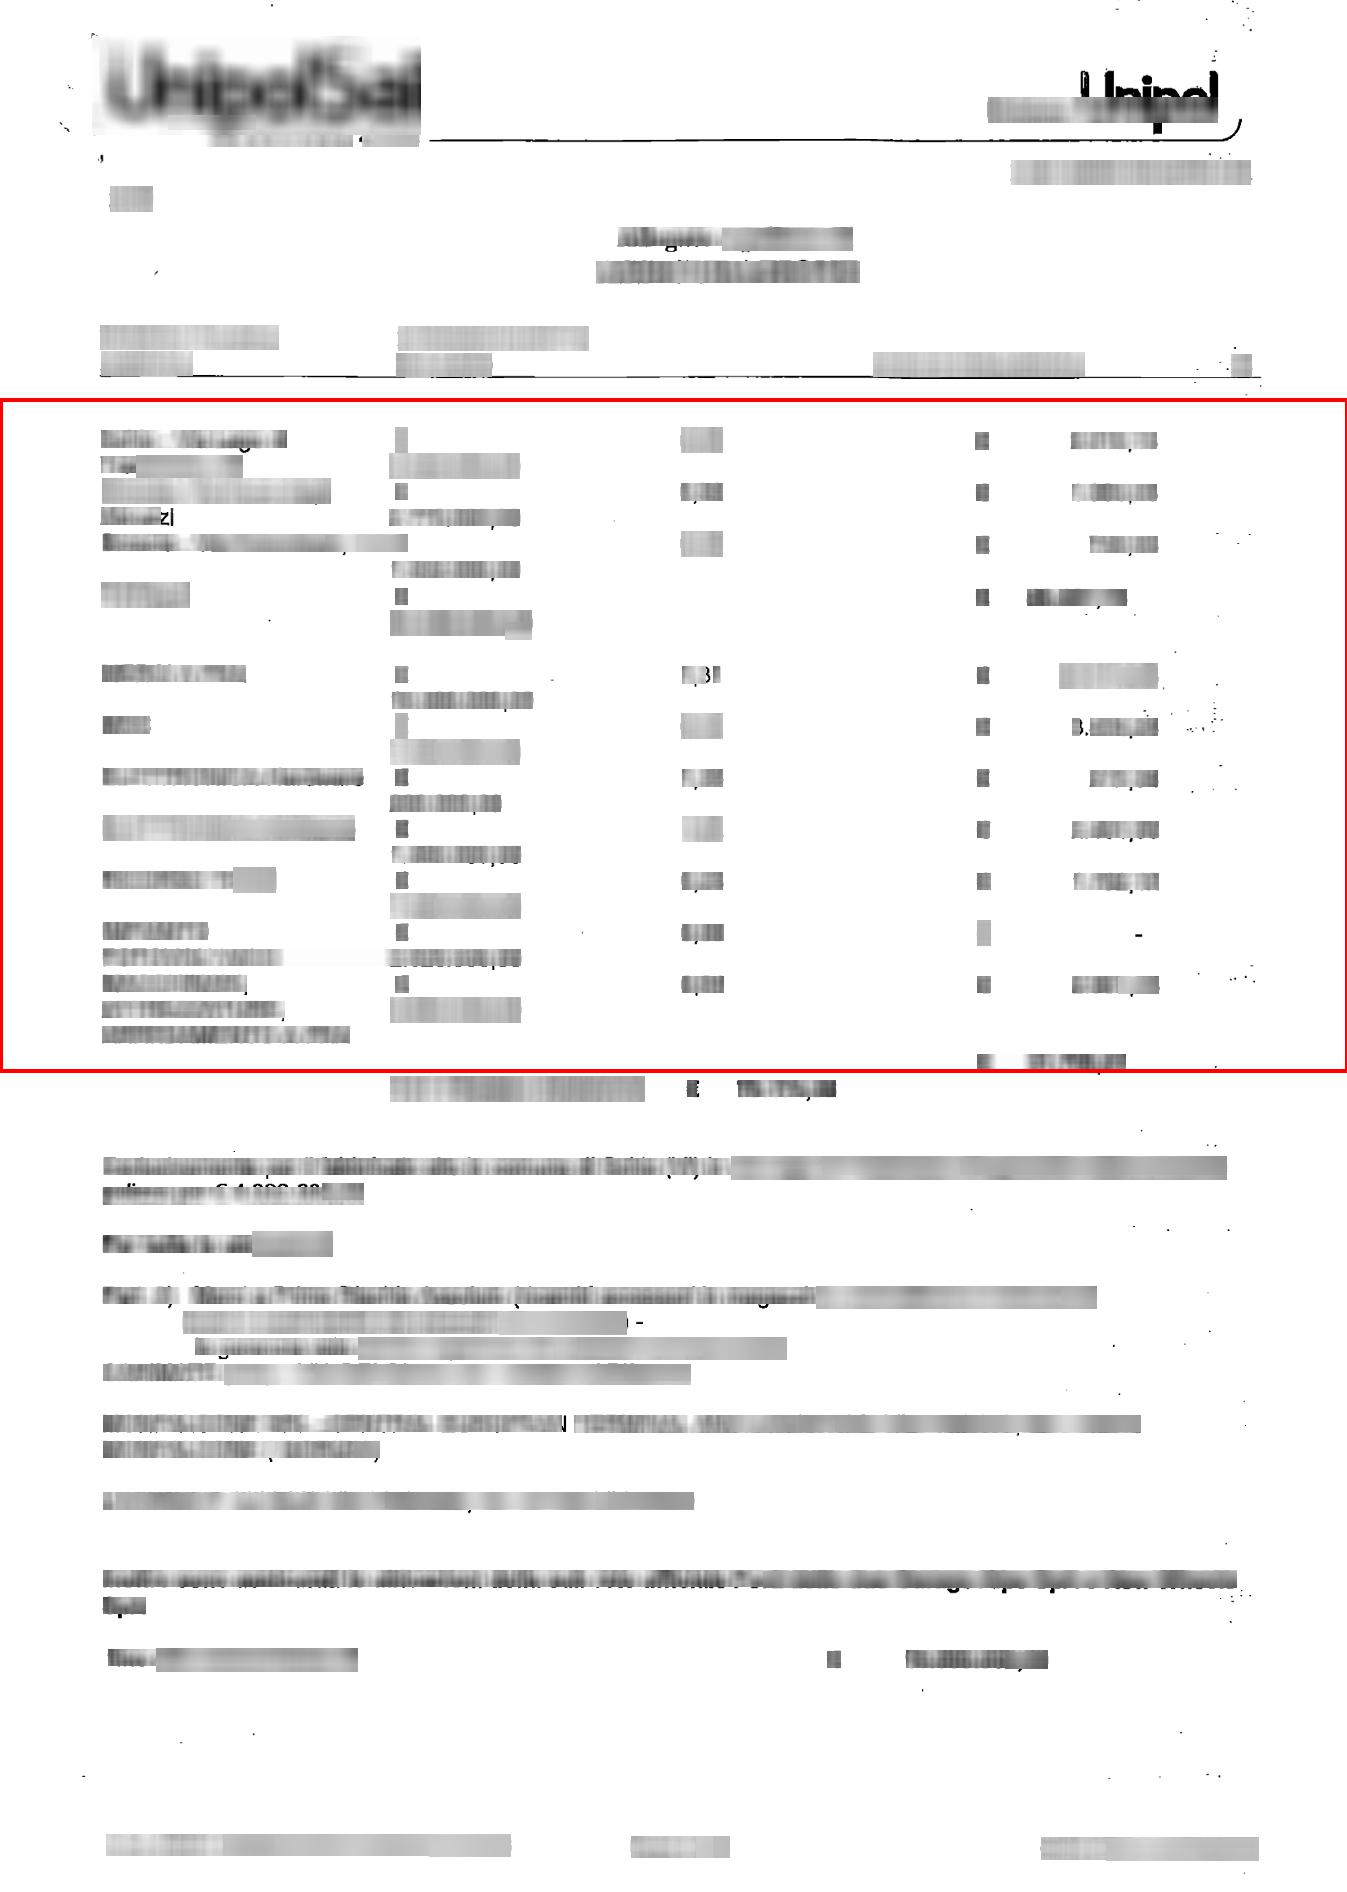
\includegraphics[width=1\columnwidth]{appendice/unite/test0_merged_0_6_momentum_1}  
    \end{minipage}  
    \caption{Test 0, configurazione 4}
\end{figure}%  
Configurazione:
\begin{multicols}{2}
    \begin{lstlisting}
image_resizer {
  fixes_shape_resizer {
    width: 400
    heigth: 400
  }
}
first_stage_box_predictor {
  l2_regularizer {
    weight: 0.00001
}
first_stage_nms_iou_threshold: 0.7
second_stage_box_predictor {
  l2_regularizer {
    weight: 0.00004
  }
}
second_stage_post_processing {
  iou_threshold: 0.6
}
optimizer {
  adam_optimizer: {
    learning_rate: {
      manual_step_learning_rate {
        initial_learning_rate: 0.0008
        schedule {
          step: 4500
          learning_rate: .0008
        }
        schedule {
          step: 7000
          learning_rate: .0004
        }
        schedule {
          step: 10000
          learning_rate: .00008
        }
    ...
    }
    momentum_optimizer_value: 0.9
  }
  use_moving_average: false
}
    \end{lstlisting}
\end{multicols}
%============================================================================================

\newpage
\begin{figure}[H]  
    \begin{minipage}{.5\columnwidth}  
        \centering  
        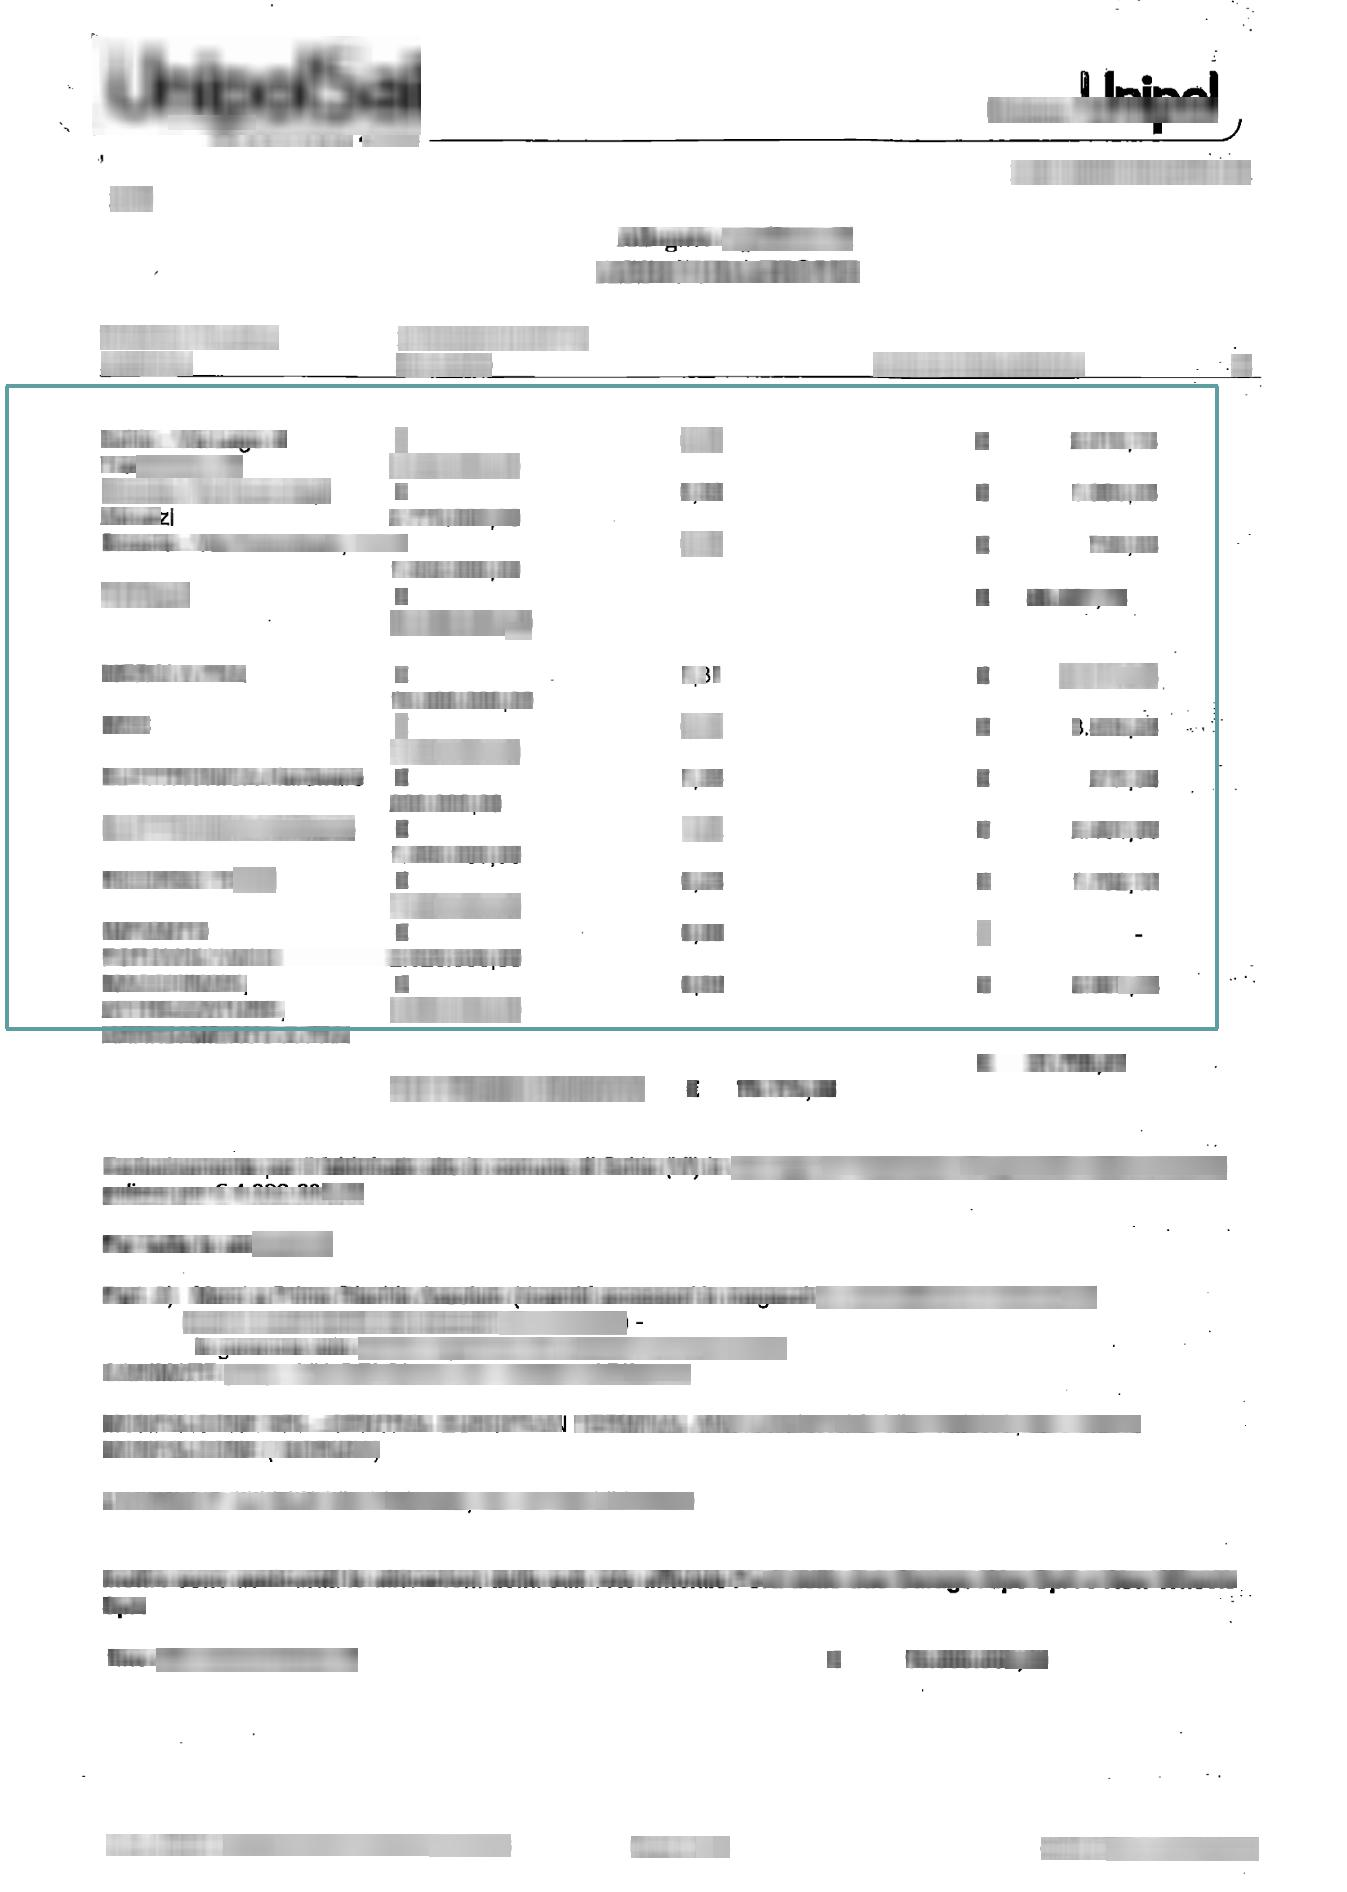
\includegraphics[width=1\columnwidth]{appendice/filtrate/test0_filtered_0_6_momentum_10k_jpg}  
    \end{minipage}%  
    \begin{minipage}{0.5\columnwidth}  
        \centering  
        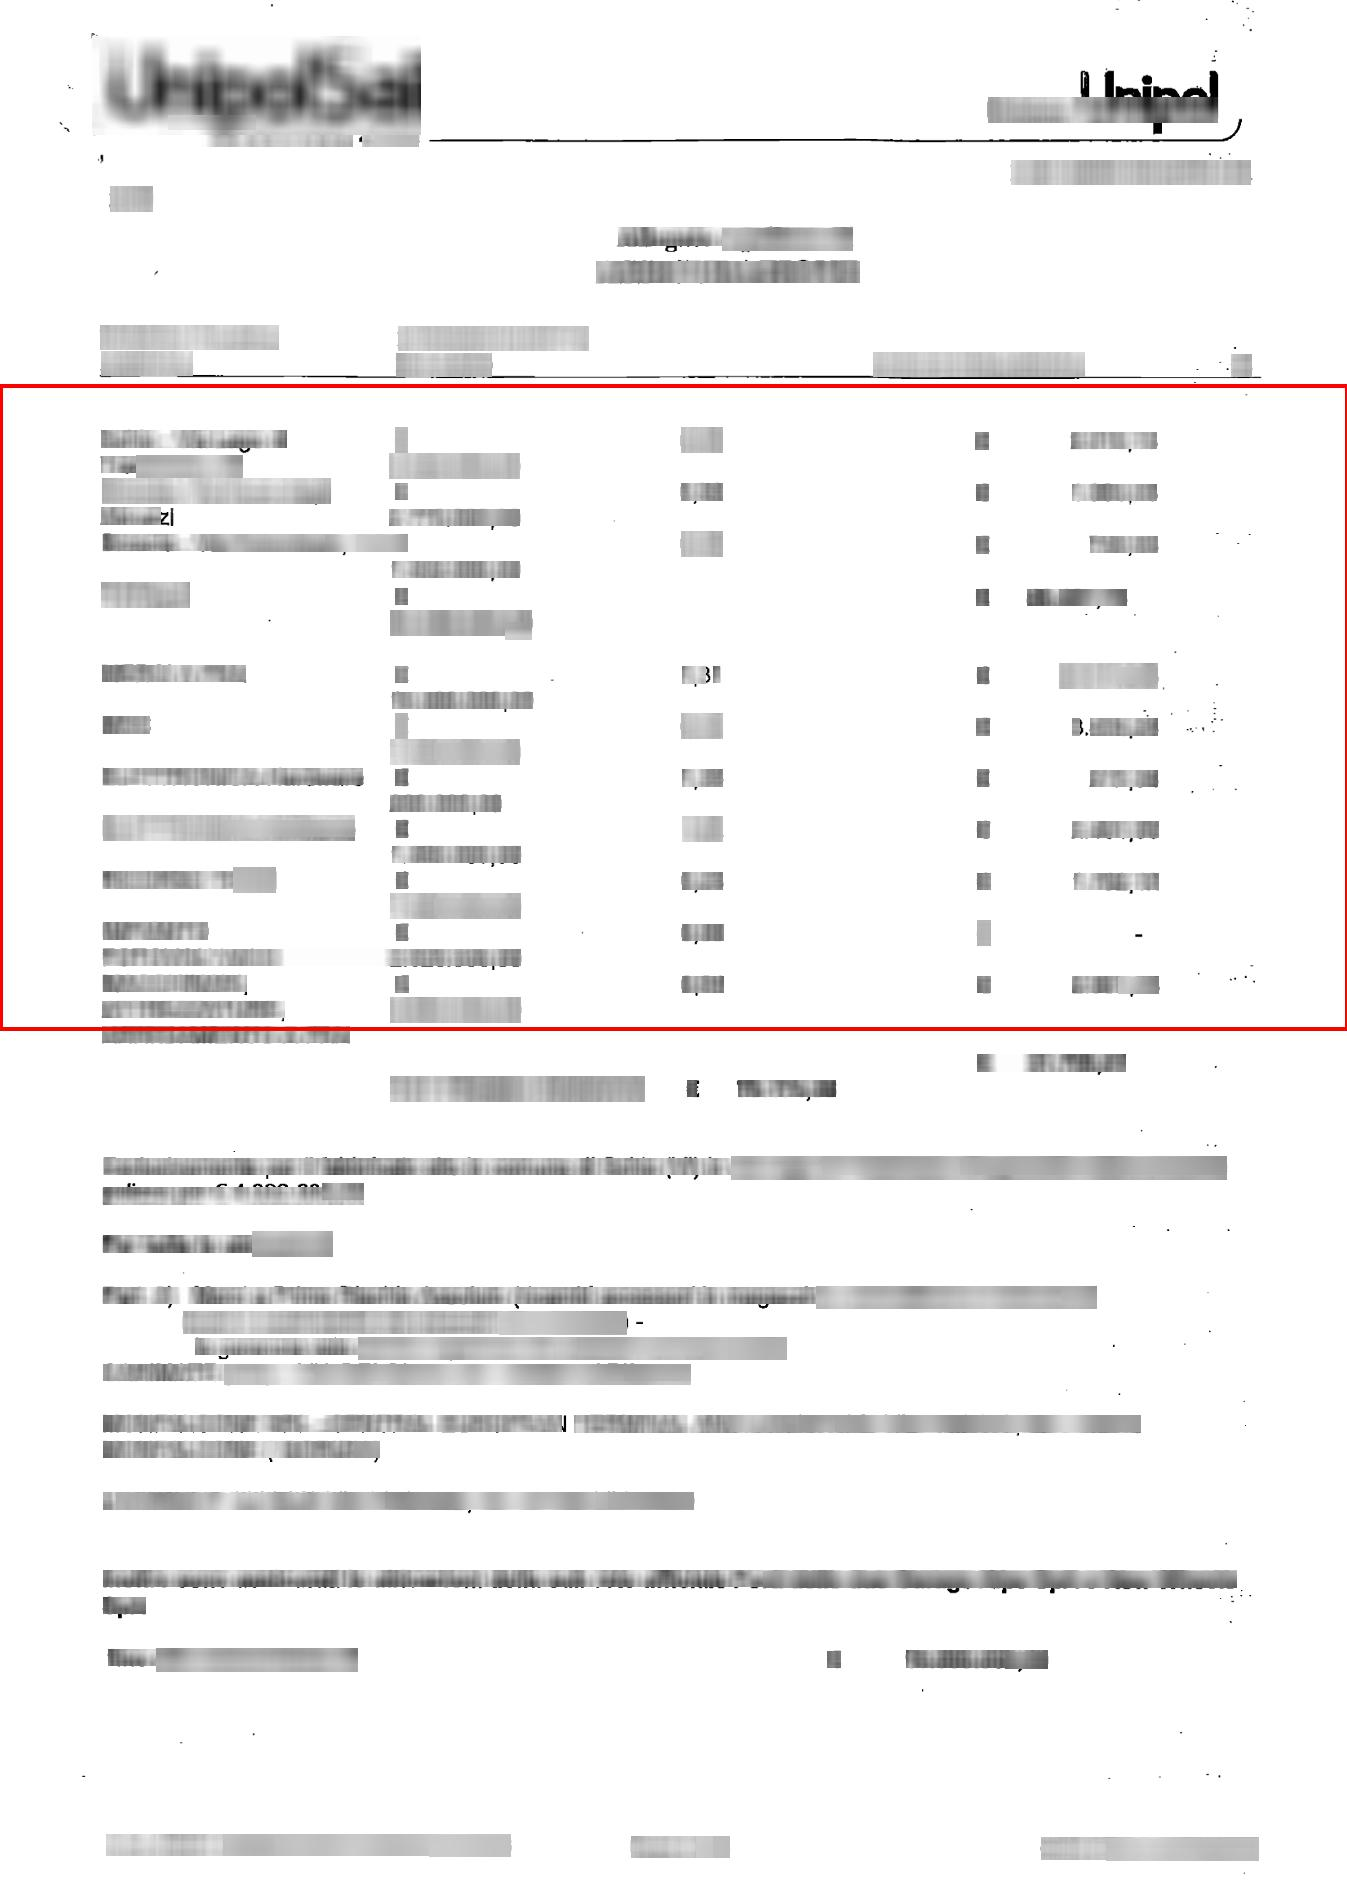
\includegraphics[width=1\columnwidth]{appendice/unite/test0_merged_0_6_momentum_10k_jpg}  
    \end{minipage}  
    \caption{Test 0, configurazione 5}
\end{figure}%  
Configurazione:
\begin{multicols}{2}
    \begin{lstlisting}
image_resizer {
  fixes_shape_resizer {
    width: 400
    heigth: 400
  }
}
first_stage_box_predictor {
  l2_regularizer {
    weight: 0.004
}
first_stage_nms_iou_threshold: 0.7
second_stage_box_predictor {
  l2_regularizer {
    weight: 0.004
  }
}
second_stage_post_processing {
  iou_threshold: 0.6
}
optimizer {
  adam_optimizer: {
    learning_rate: {
      manual_step_learning_rate {
        initial_learning_rate: 0.0004
        schedule {
          step: 4500
          learning_rate: .0002
        }
        schedule {
          step: 7000
          learning_rate: .00002
        }
        schedule {
          step: 10000
          learning_rate: .000002
        }
    ...
    }
    momentum_optimizer_value: 0.9
  }
  use_moving_average: false
}
    \end{lstlisting}
\end{multicols}
%============================================================================================

\newpage
\begin{figure}[H]  
    \begin{minipage}{.5\columnwidth}  
        \centering  
        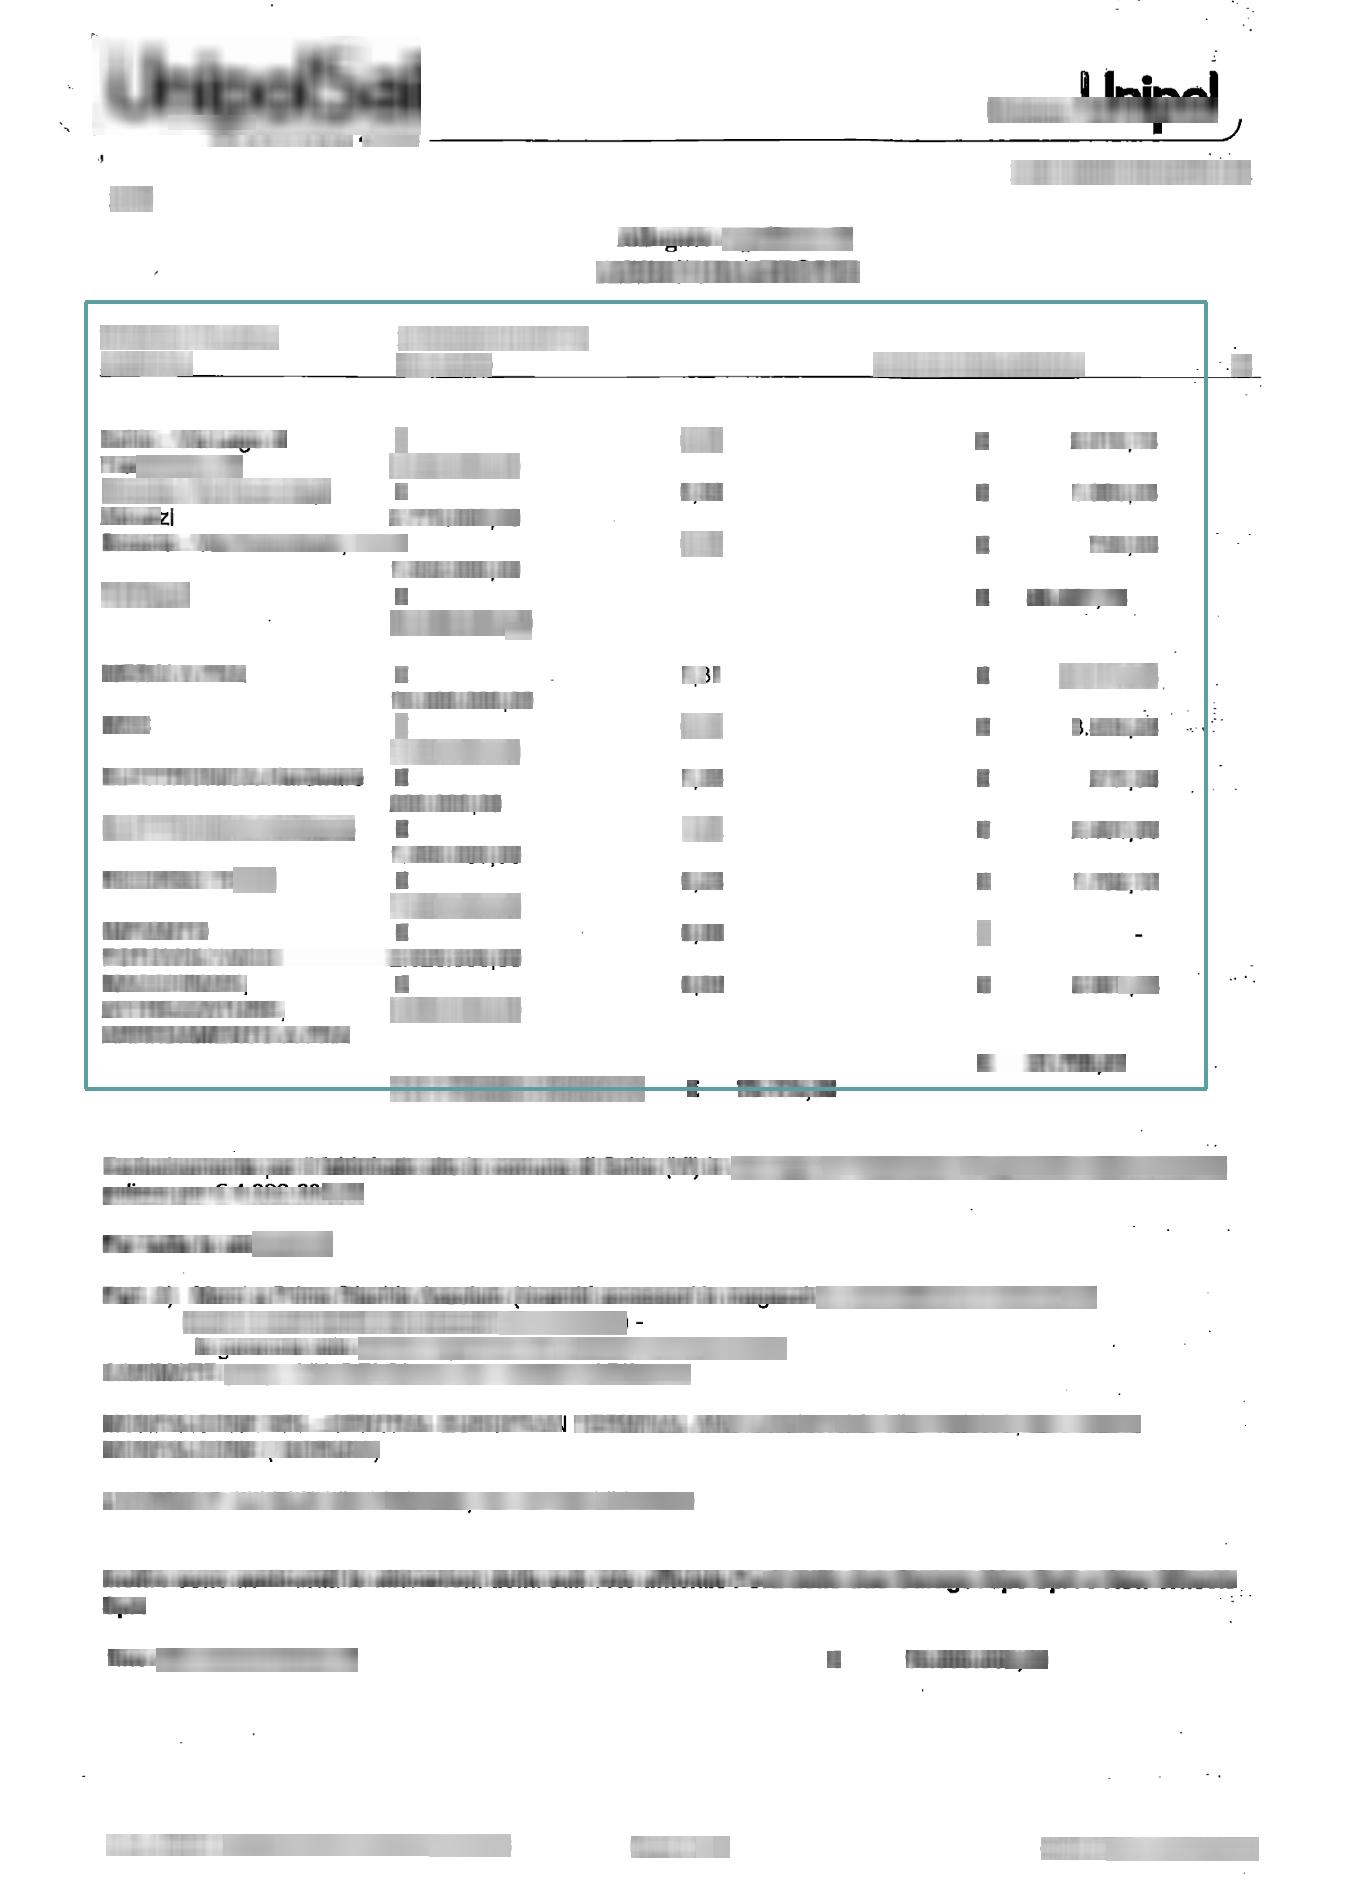
\includegraphics[width=1\columnwidth]{appendice/filtrate/test0_filtered_0_6_momentum_optimizer_1batch}  
    \end{minipage}%  
    \begin{minipage}{0.5\columnwidth}  
        \centering  
        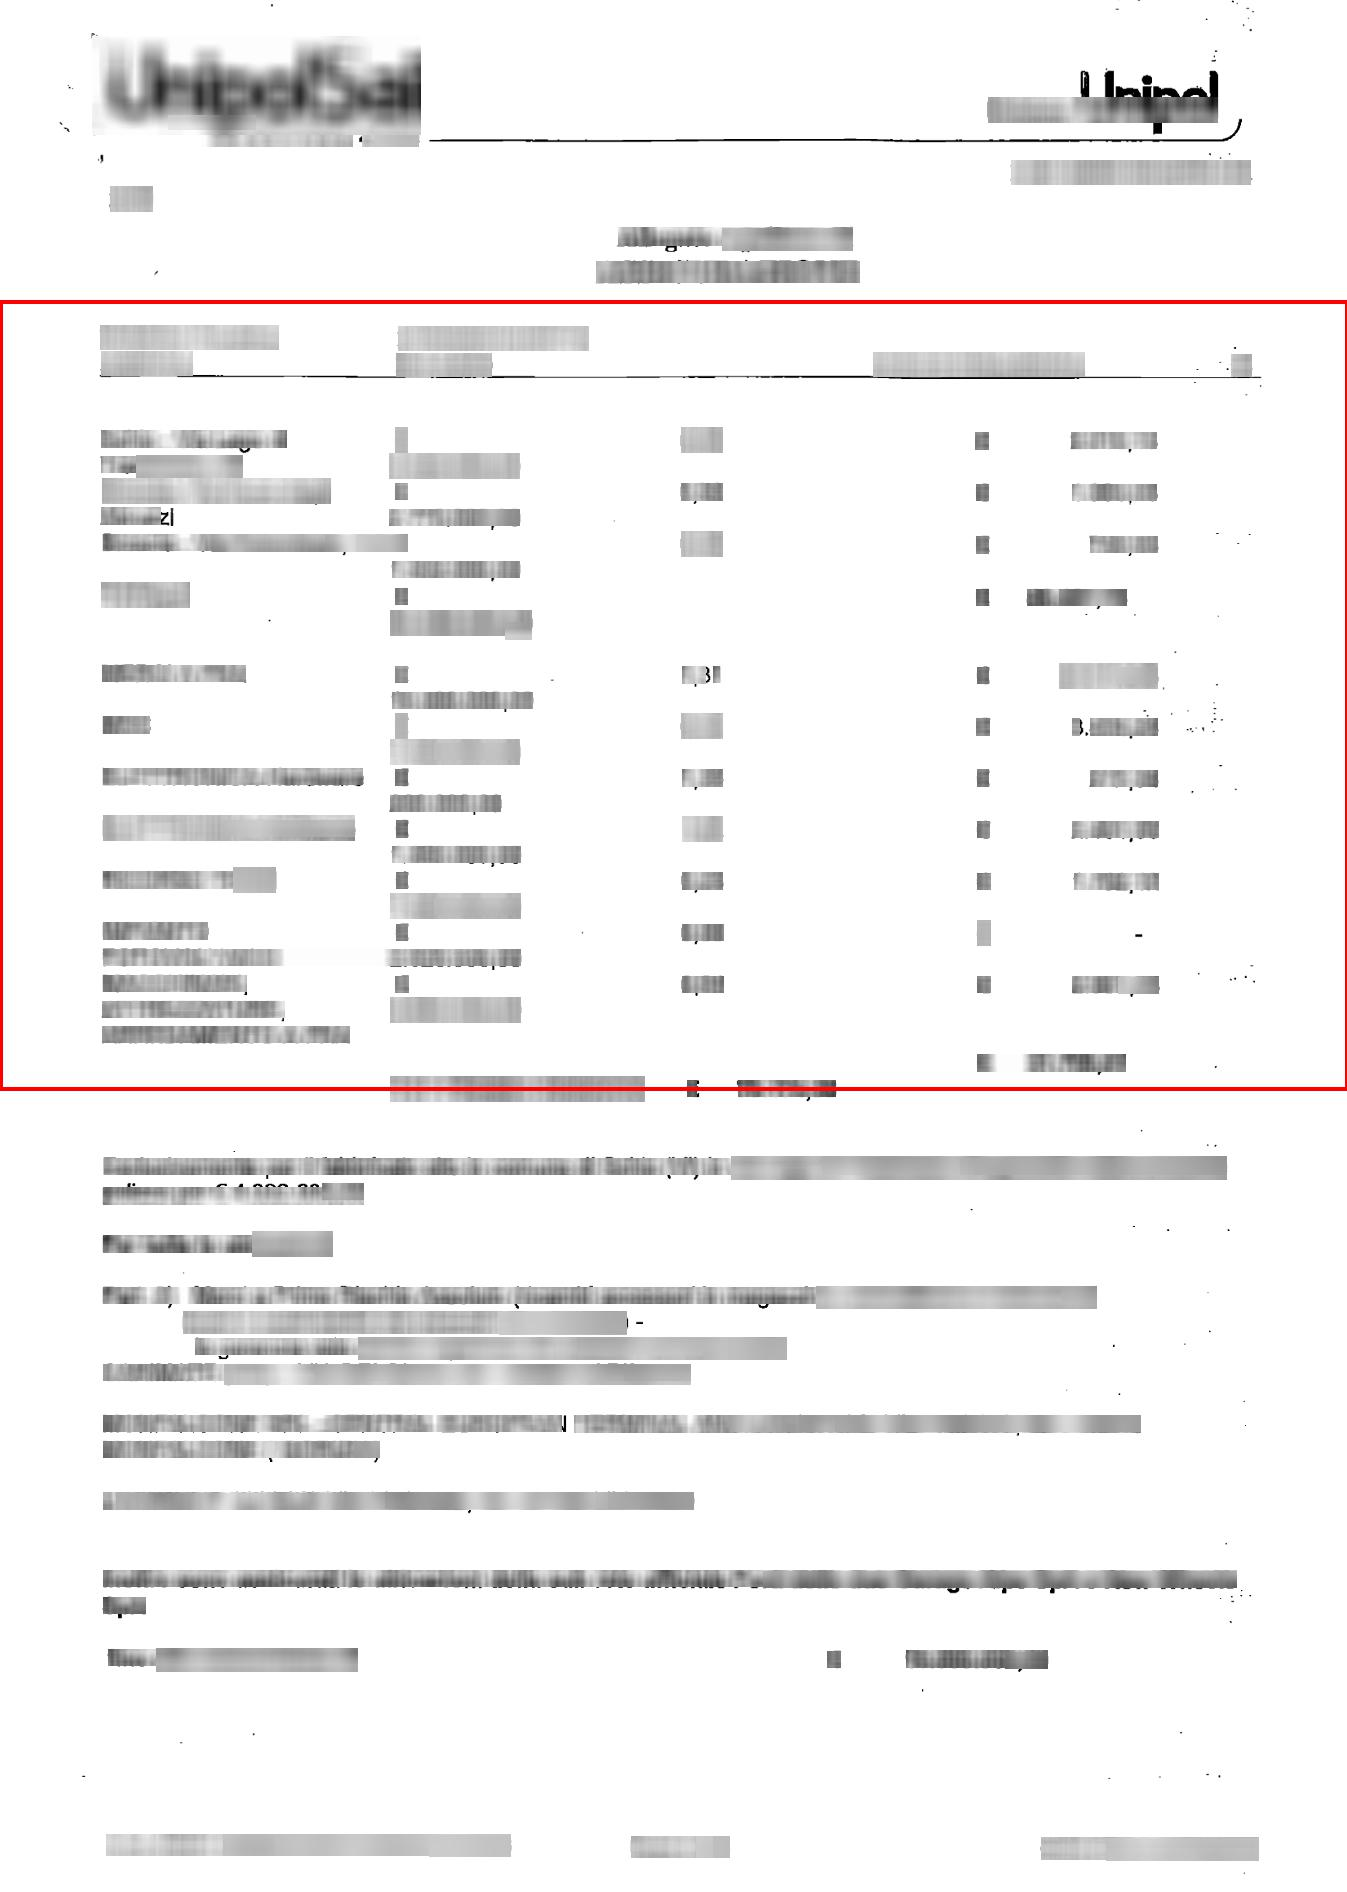
\includegraphics[width=1\columnwidth]{appendice/unite/test0_merged_0_6_momentum_optimizer_1batch}  
    \end{minipage}  
    \caption{Test 0, configurazione 6}
\end{figure}%  
Configurazione:
\begin{multicols}{2}
    \begin{lstlisting}
image_resizer {
  fixes_shape_resizer {
    width: 400
    heigth: 400
  }
}
first_stage_box_predictor {
  l2_regularizer {
    weight: 0.04
}
first_stage_nms_iou_threshold: 0.7
second_stage_box_predictor {
  l2_regularizer {
    weight: 0.004
  }
}
second_stage_post_processing {
  iou_threshold: 0.6
}
batch_size: 1
optimizer {
  adam_optimizer: {
    learning_rate: {
      manual_step_learning_rate {
        initial_learning_rate: 0.0004
        schedule {
          step: 4500
          learning_rate: .0002
        }
        schedule {
          step: 7000
          learning_rate: .00002
        }
        schedule {
          step: 10000
          learning_rate: .000002
        }
    ...
    }
    momentum_optimizer_value: 0.9
  }
  use_moving_average: false
}
    \end{lstlisting}
\end{multicols}
%============================================================================================
\newpage
\subsection{Test 1}
\begin{figure}[!ht] 
    \centering
    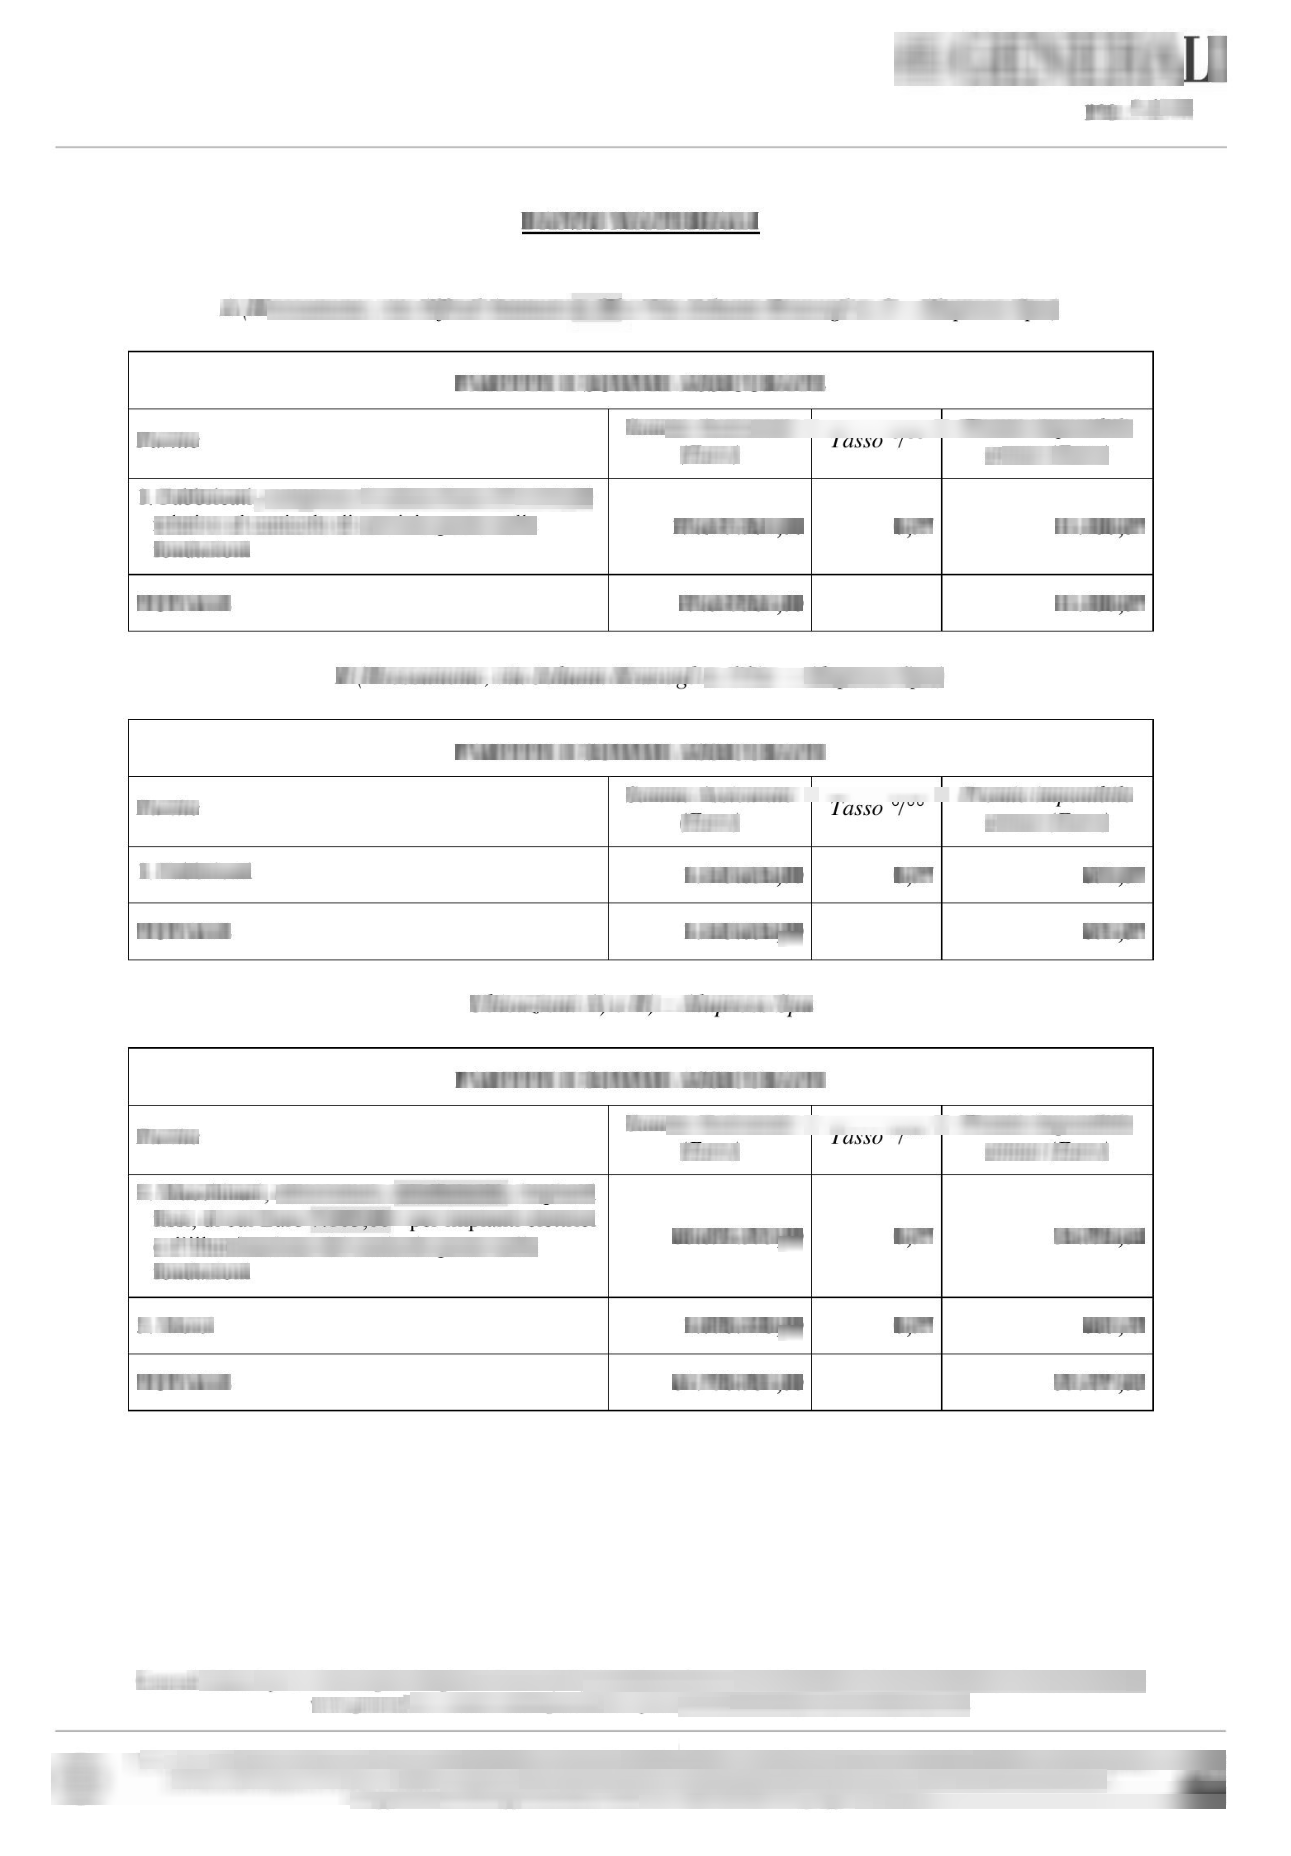
\includegraphics[width=1\columnwidth]{appendice/test1} 
    \caption{Test 1}
    \label{img:test-1}
\end{figure} 
\newpage

%============================================================================================


\begin{figure}[H]  
    \begin{minipage}{.5\columnwidth}  
        \centering  
        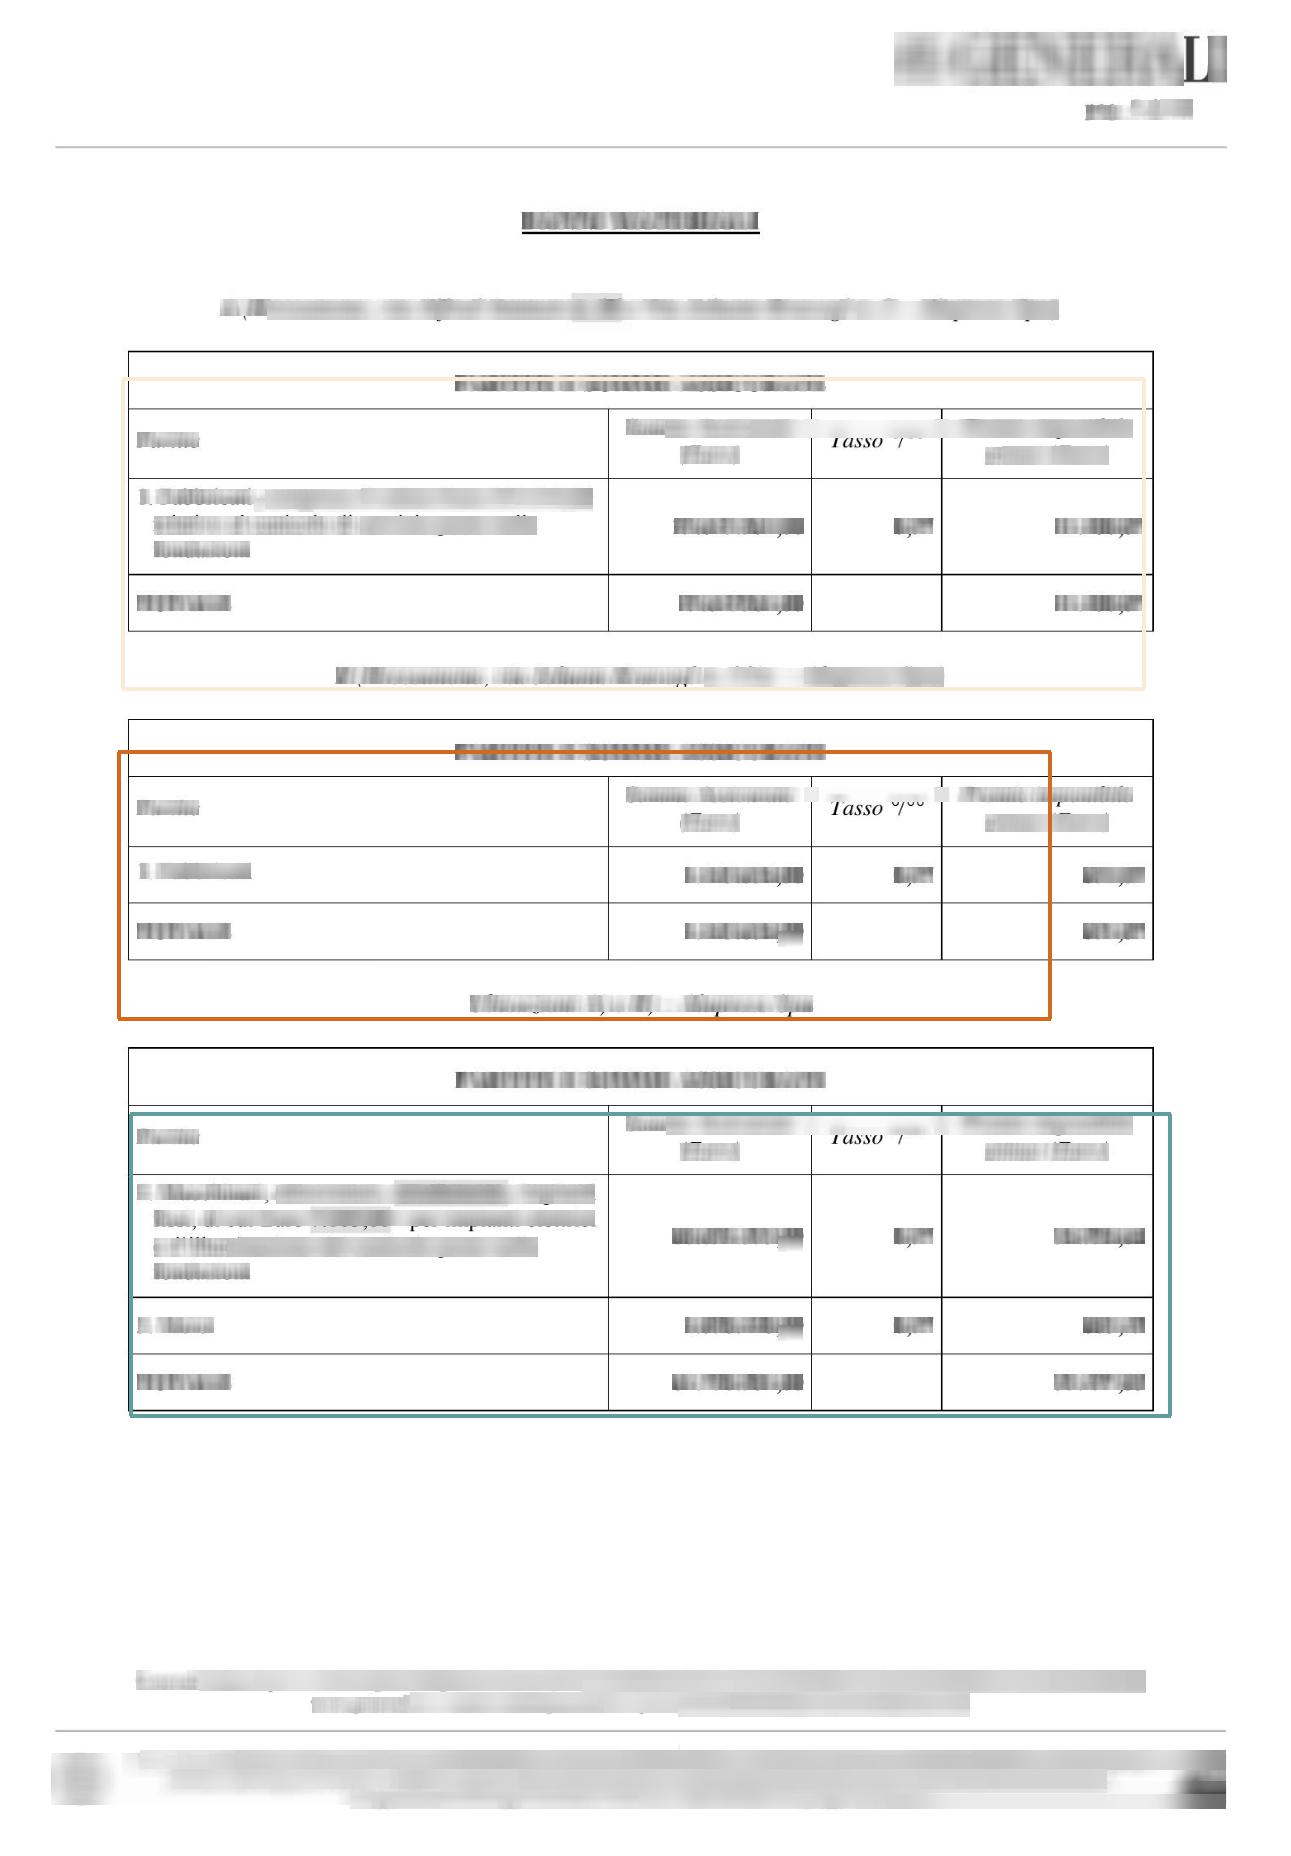
\includegraphics[width=1\columnwidth]{appendice/filtrate/test1_filtered_0_6_adam_1}  
    \end{minipage}%  
    \begin{minipage}{0.5\columnwidth}  
        \centering  
        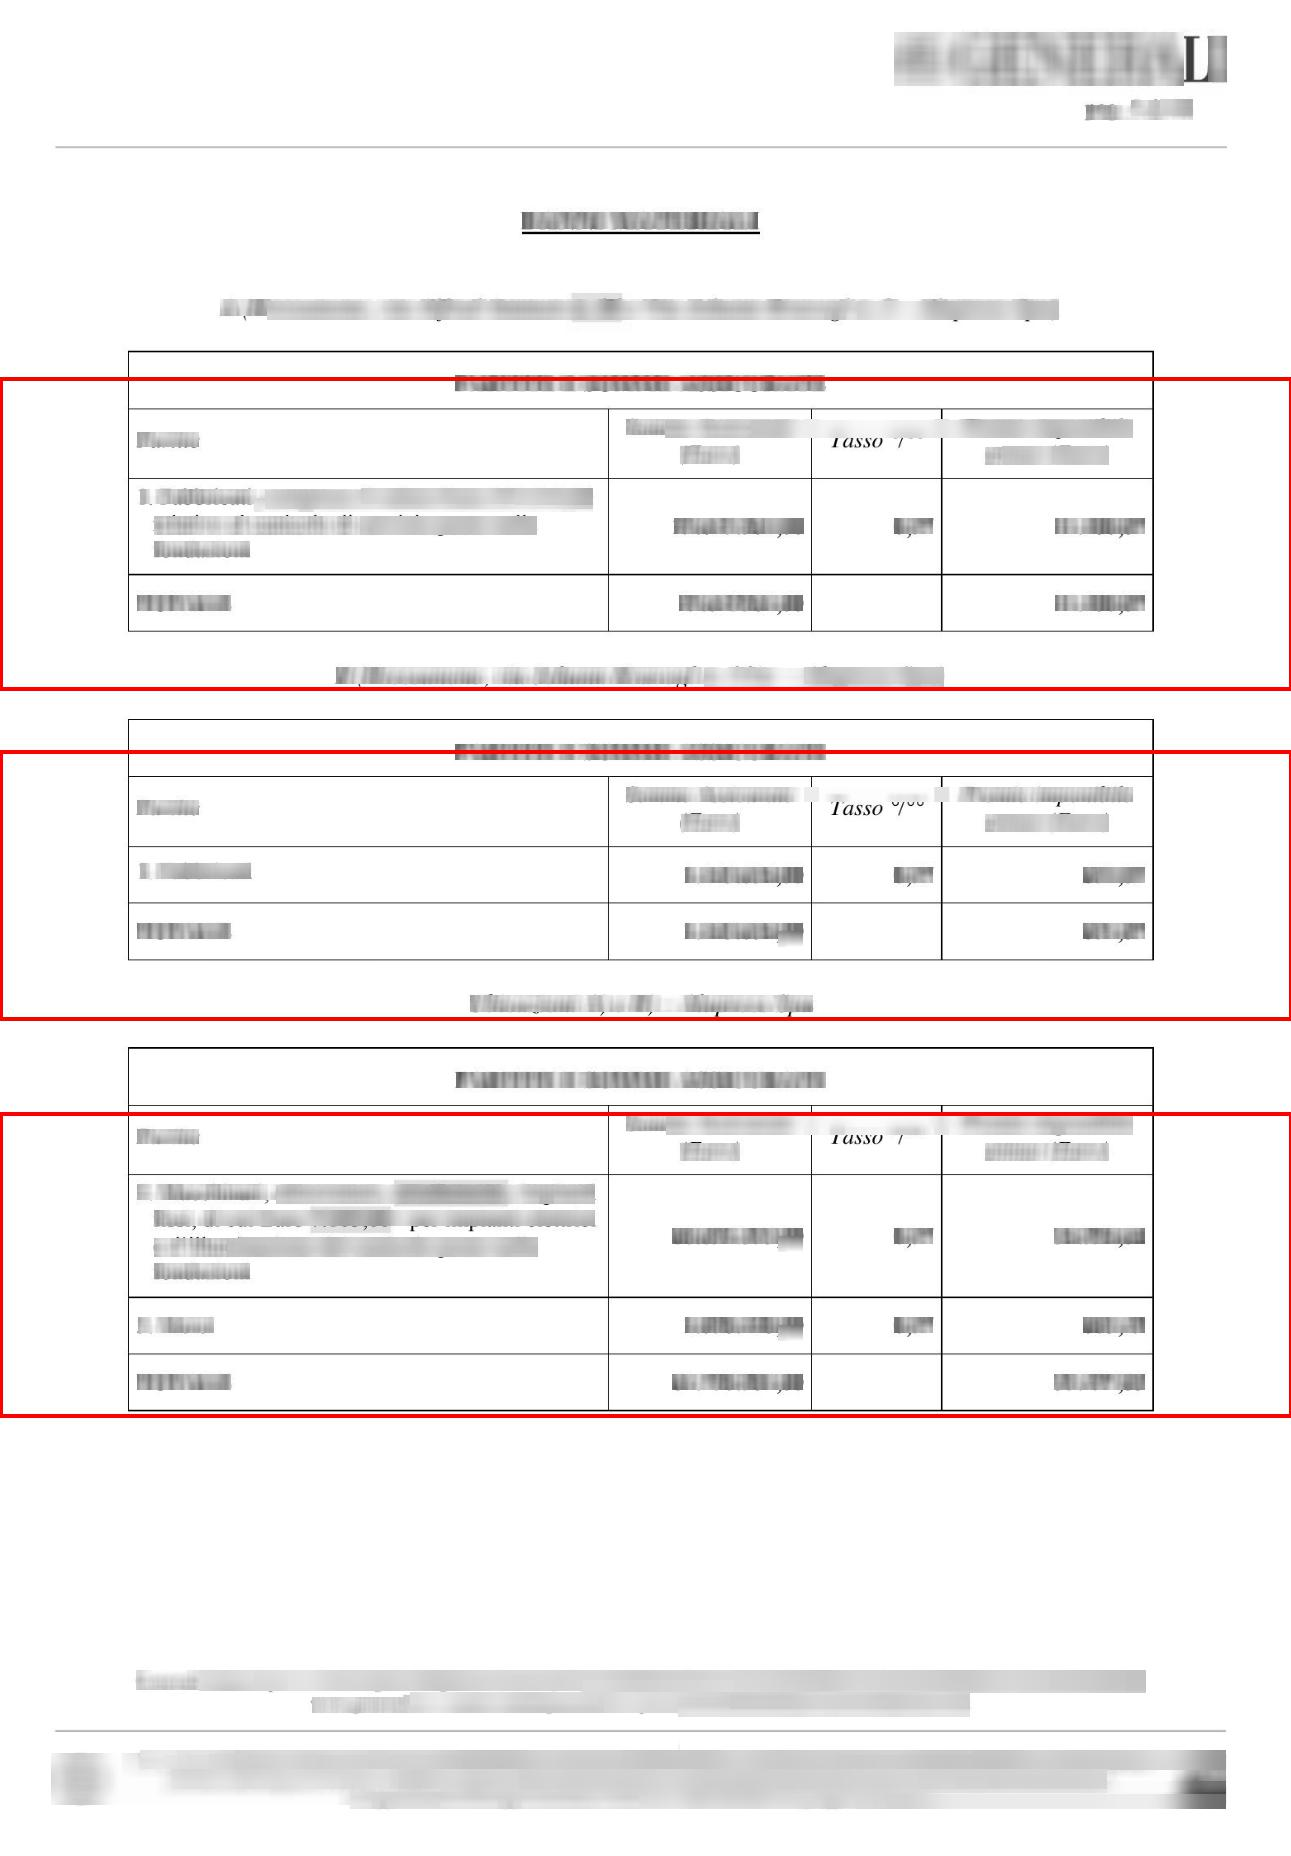
\includegraphics[width=1\columnwidth]{appendice/unite/test1_merged_0_6_adam_1}  
    \end{minipage}  
    \caption{Test 1, configurazione 1}
\end{figure}%  
Configurazione:
\begin{multicols}{2}
    \begin{lstlisting}
image_resizer {
  fixes_shape_resizer {
    width: 400
    heigth: 400
  }
}
first_stage_box_predictor {
  l2_regularizer {
    weight: 0.008
}
first_stage_nms_iou_threshold: 0.7
second_stage_box_predictor {
  l2_regularizer {
    weight: 0.004
  }
}
second_stage_post_processing {
  iou_threshold: 0.6
}
optimizer {
  adam_optimizer: {
    learning_rate: {
      manual_step_learning_rate {
        initial_learning_rate: .00008
        schedule {
          step: 4500
          learning_rate: .00004
        }
        schedule {
          step: 7000
          learning_rate: .00002
        }
        schedule {
          step: 10000
          learning_rate: .000008
        }
    ...
    }
    momentum_optimizer_value: 0.9
  }
  use_moving_average: false
}
\end{lstlisting}
\end{multicols}

%============================================================================================
\newpage
\begin{figure}[H]  
    \begin{minipage}{.5\columnwidth}  
        \centering  
        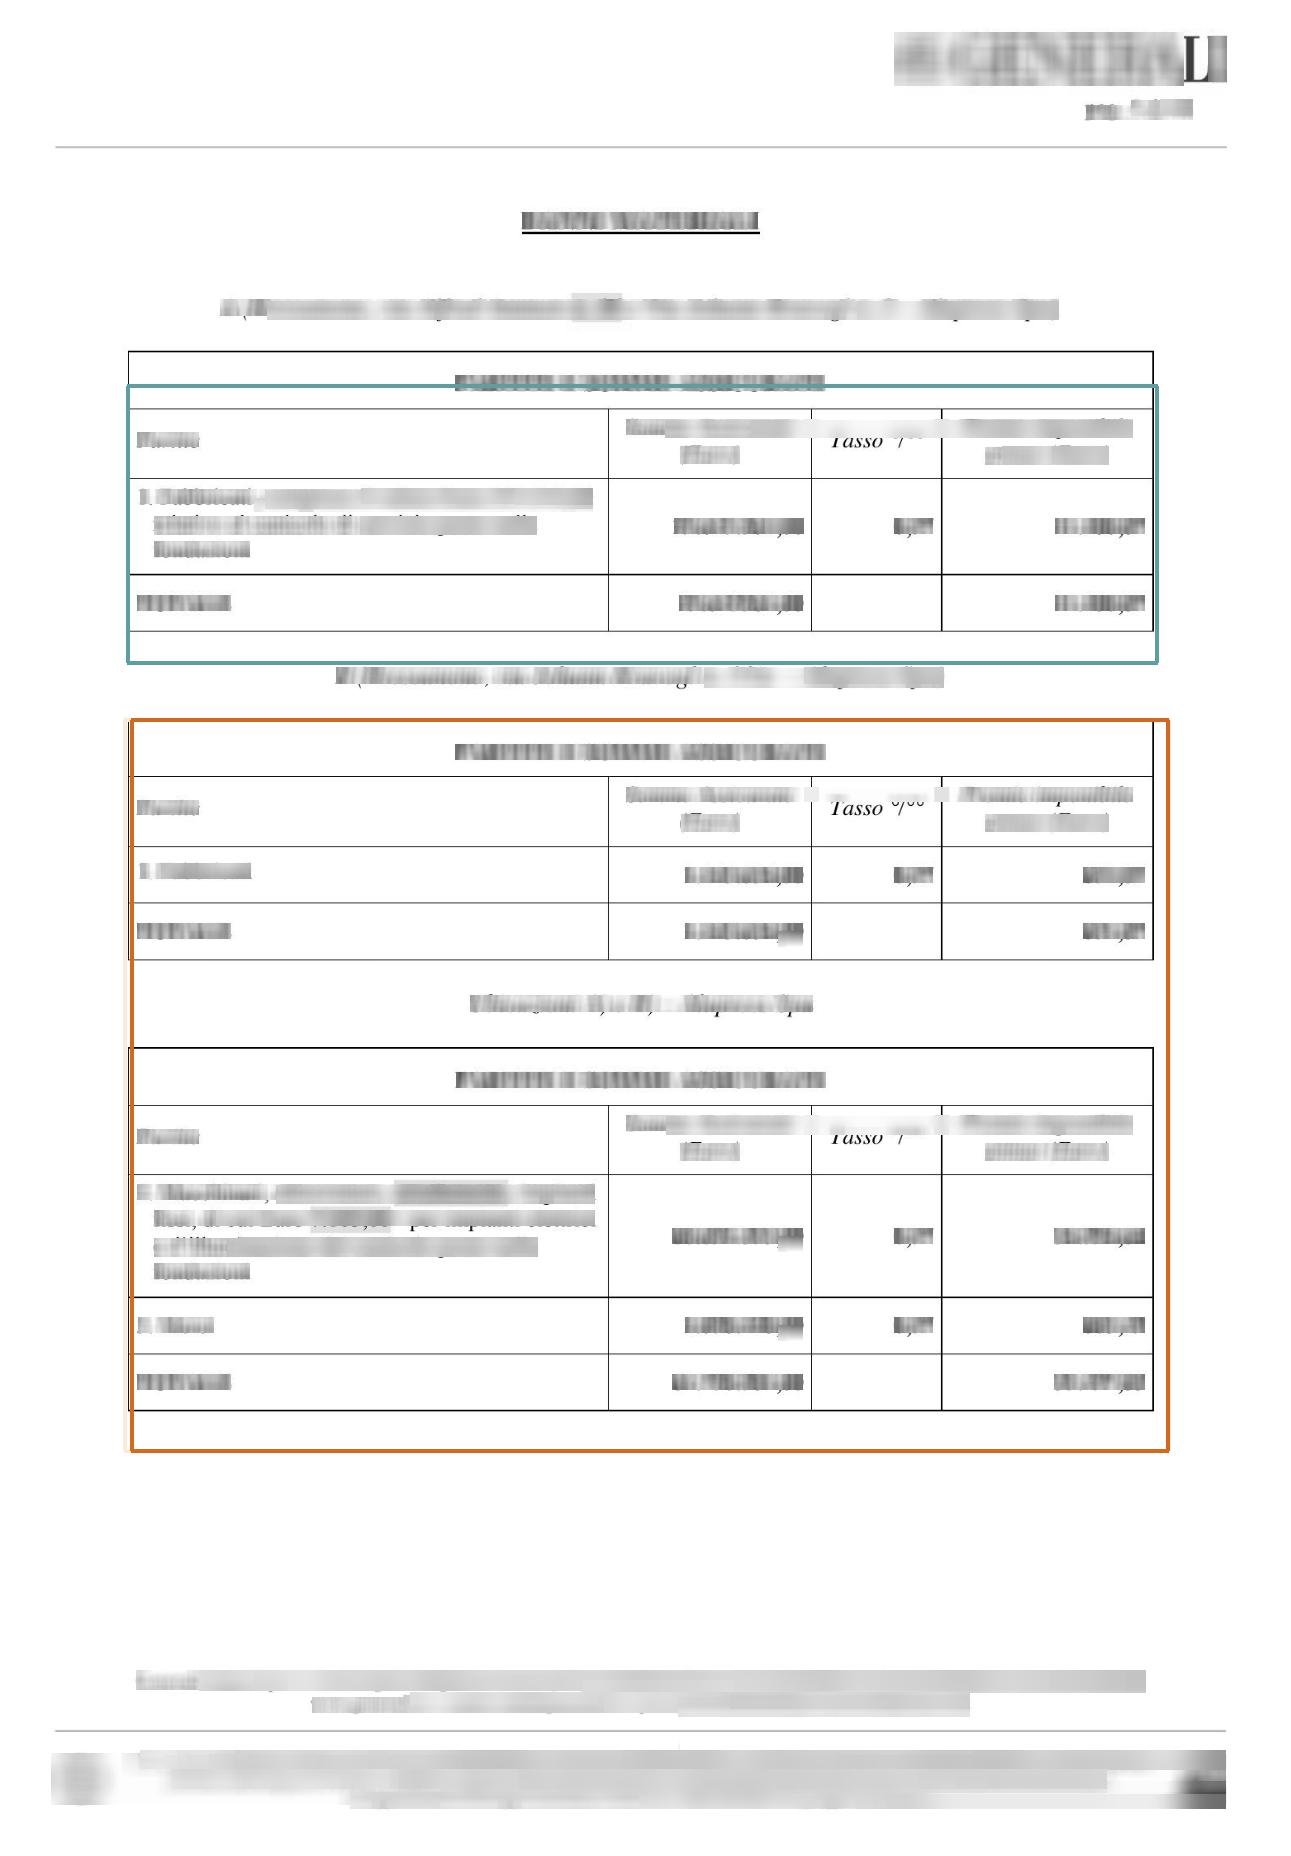
\includegraphics[width=1\columnwidth]{appendice/filtrate/test1_filtered_0_6_adam_3}  
    \end{minipage}%  
    \begin{minipage}{0.5\columnwidth}  
        \centering  
        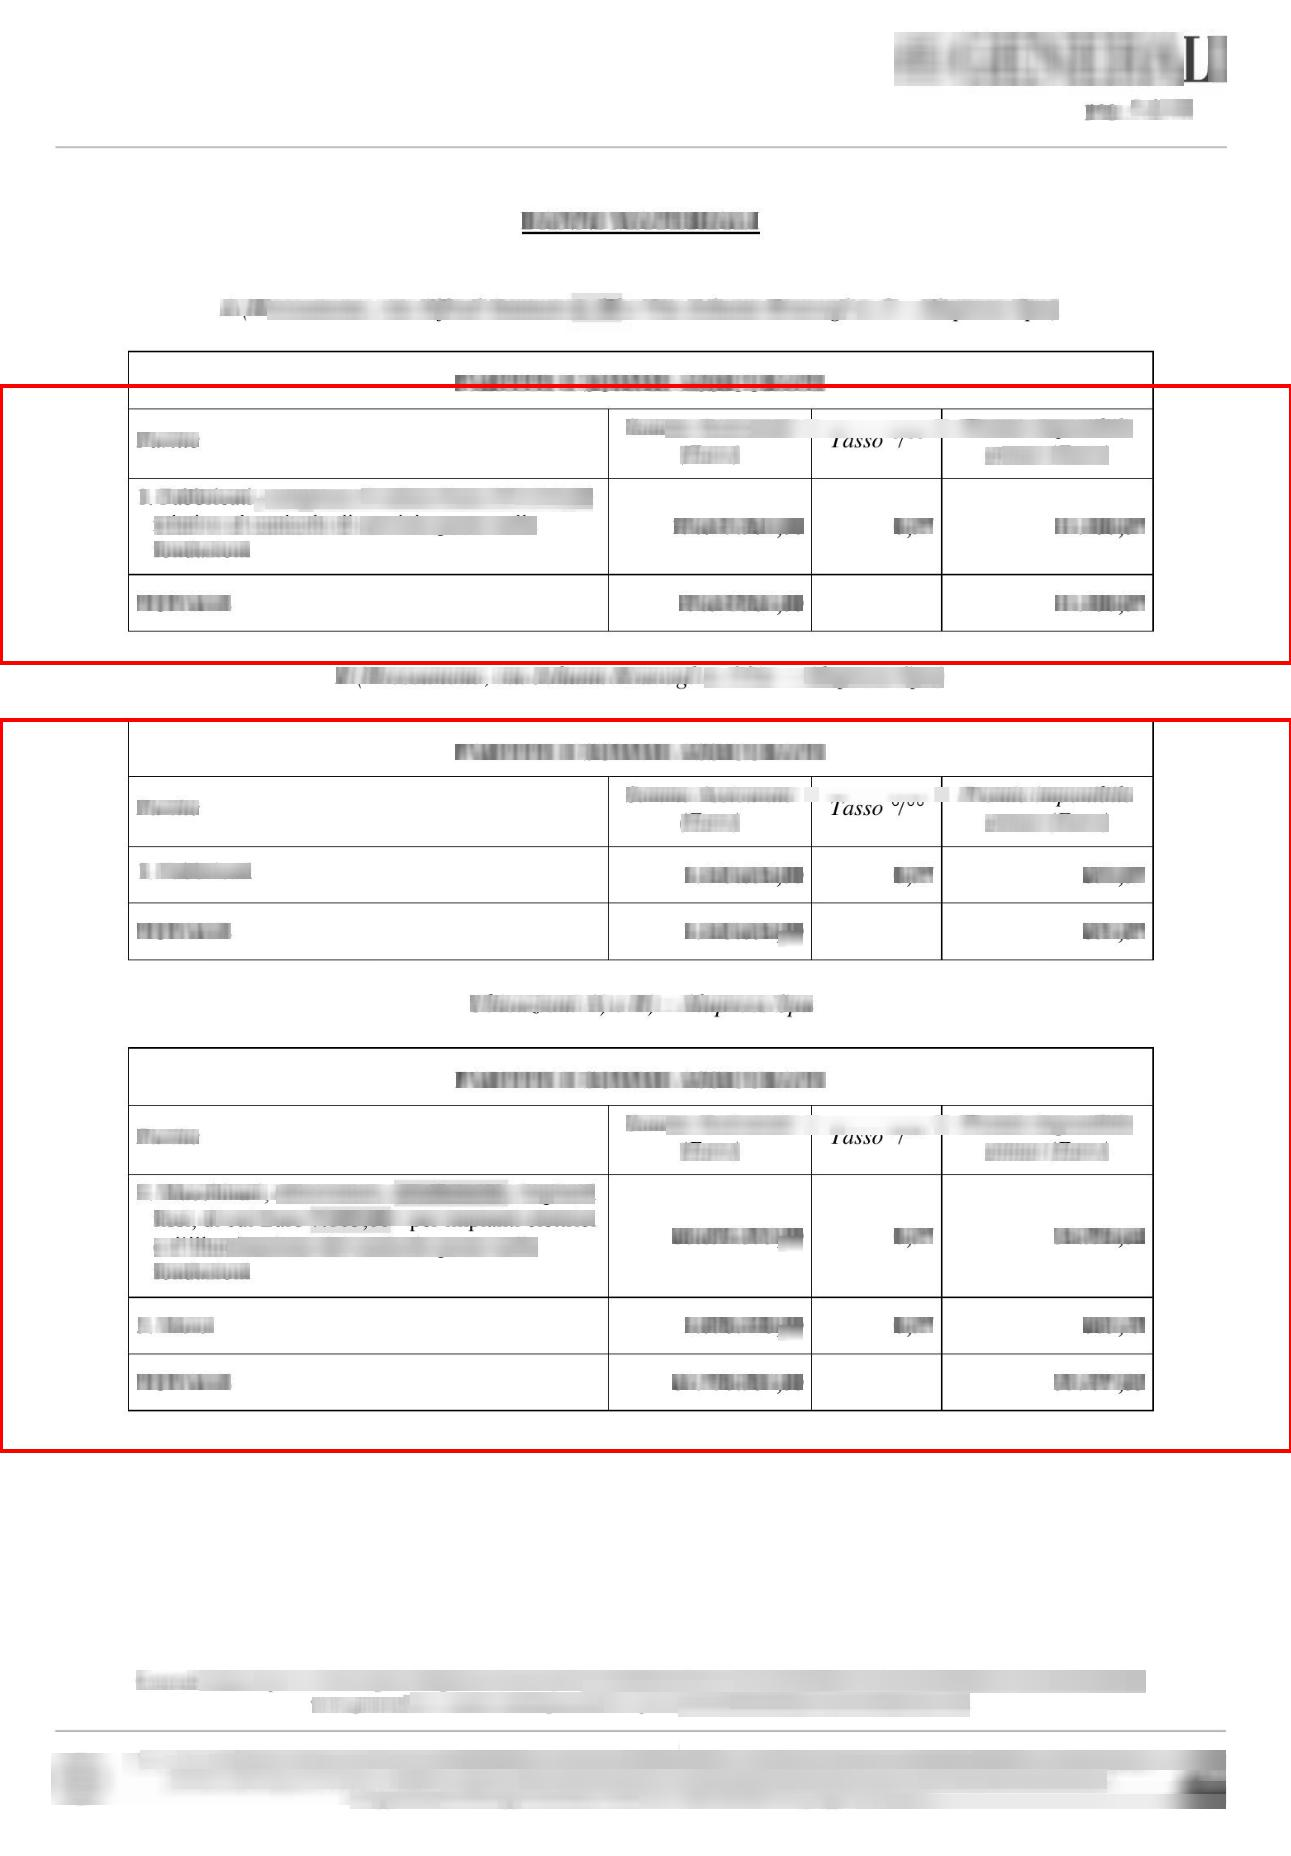
\includegraphics[width=1\columnwidth]{appendice/unite/test1_merged_0_6_adam_3}  
    \end{minipage}  
    \caption{Test 1, configurazione 2}
\end{figure}%  
Configurazione:
\begin{multicols}{2}
    \begin{lstlisting}
image_resizer {
  fixes_shape_resizer {
    width: 400
    heigth: 400
  }
}
first_stage_box_predictor {
  l2_regularizer {
    weight: 0.00001
}
first_stage_nms_iou_threshold: 0.7
second_stage_box_predictor {
  l2_regularizer {
    weight: 0.00004
  }
}
second_stage_post_processing {
  iou_threshold: 0.6
}
optimizer {
  adam_optimizer: {
    learning_rate: {
      exponential_decay_learning_rate {
        initial_learning_rate: 0.0001
          decay_steps: 600
          decay_factor: 0.95
        }
      }
    ...
  use_moving_average: false
}
    \end{lstlisting}
\end{multicols}

%============================================================================================
\newpage
\begin{figure}[H]  
    \begin{minipage}{.5\columnwidth}  
        \centering  
        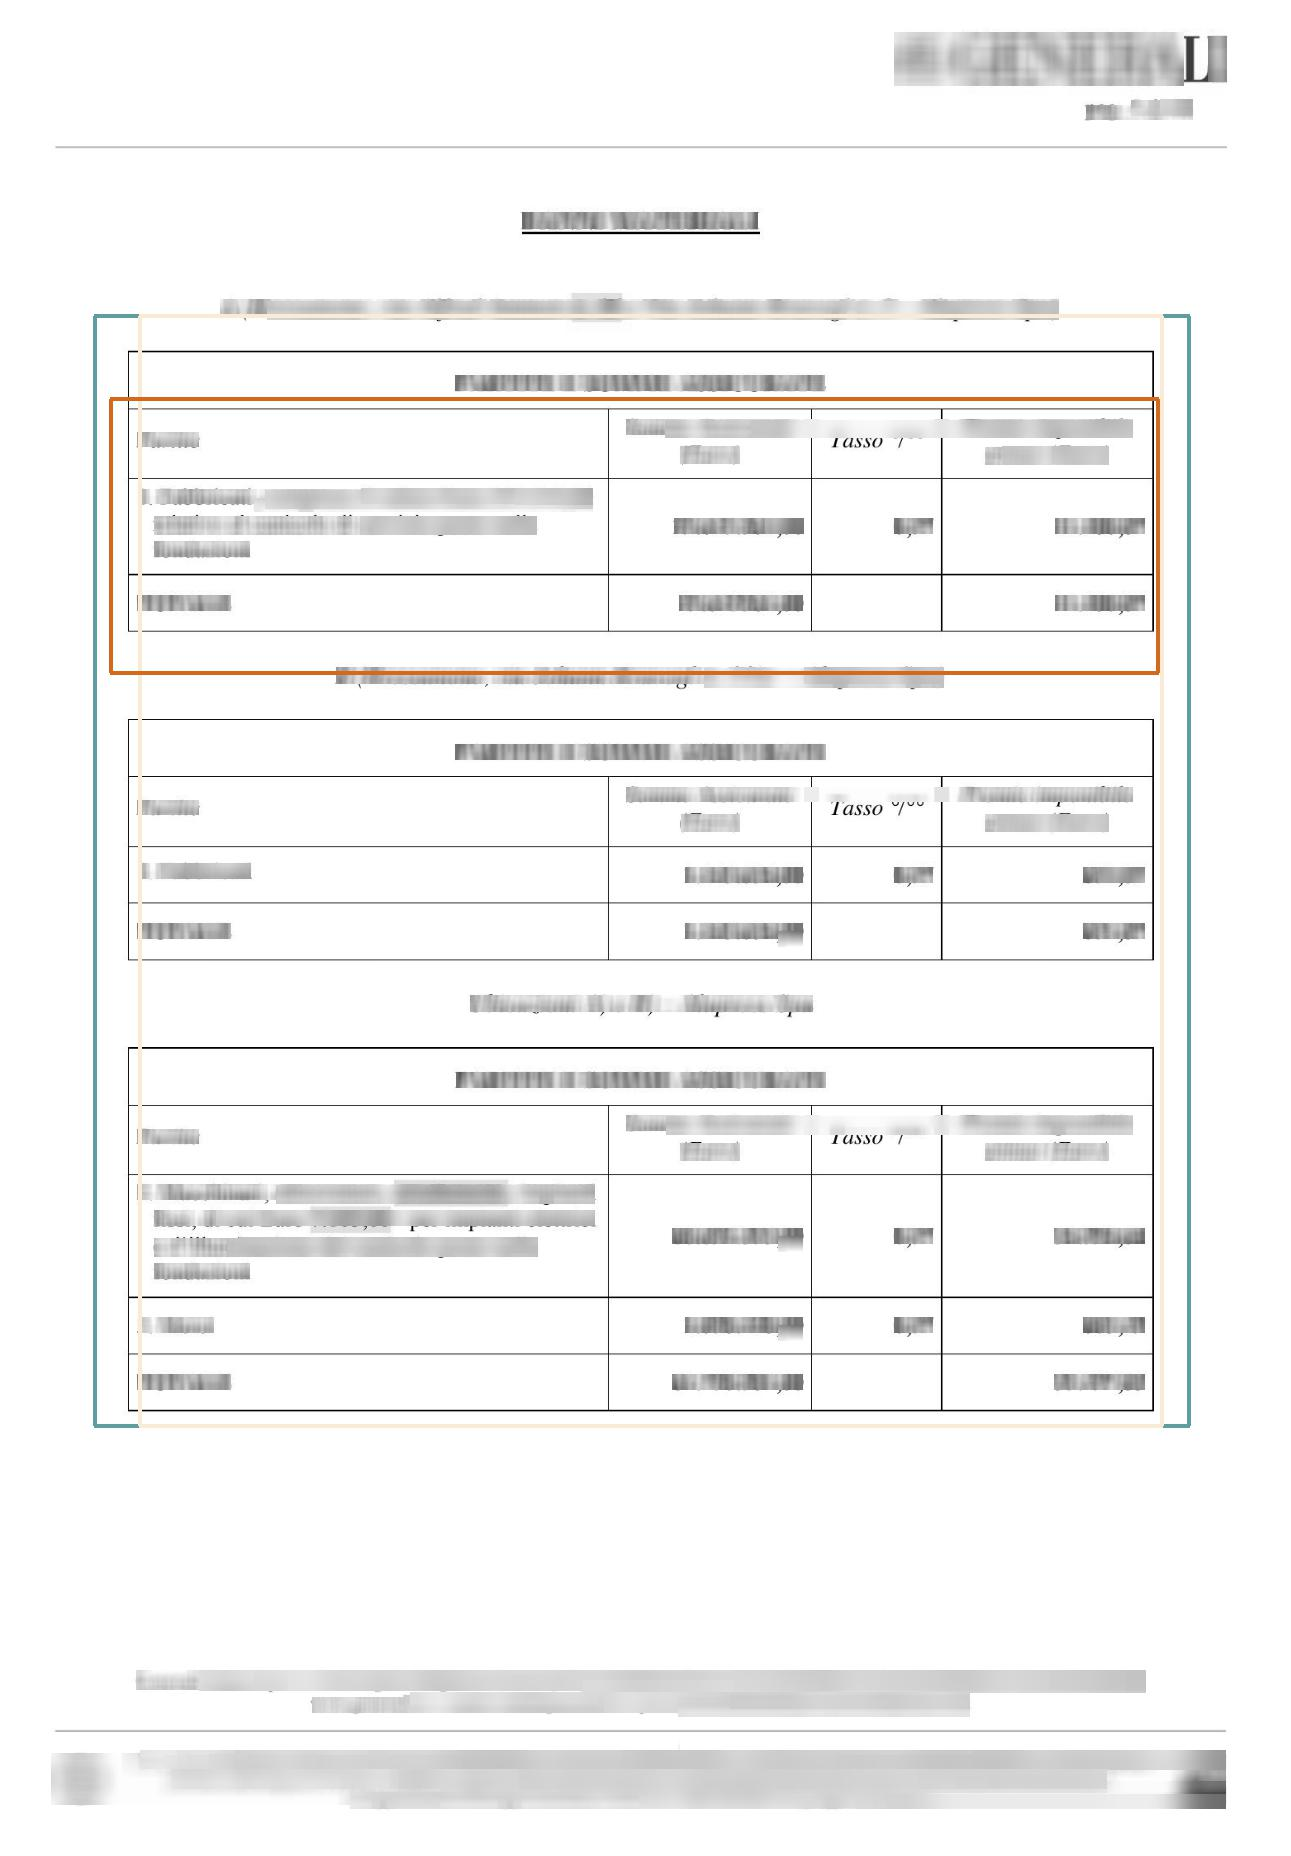
\includegraphics[width=1\columnwidth]{appendice/filtrate/test1_filtered_0_6_adam_4}  
    \end{minipage}%  
    \begin{minipage}{0.5\columnwidth}  
        \centering  
        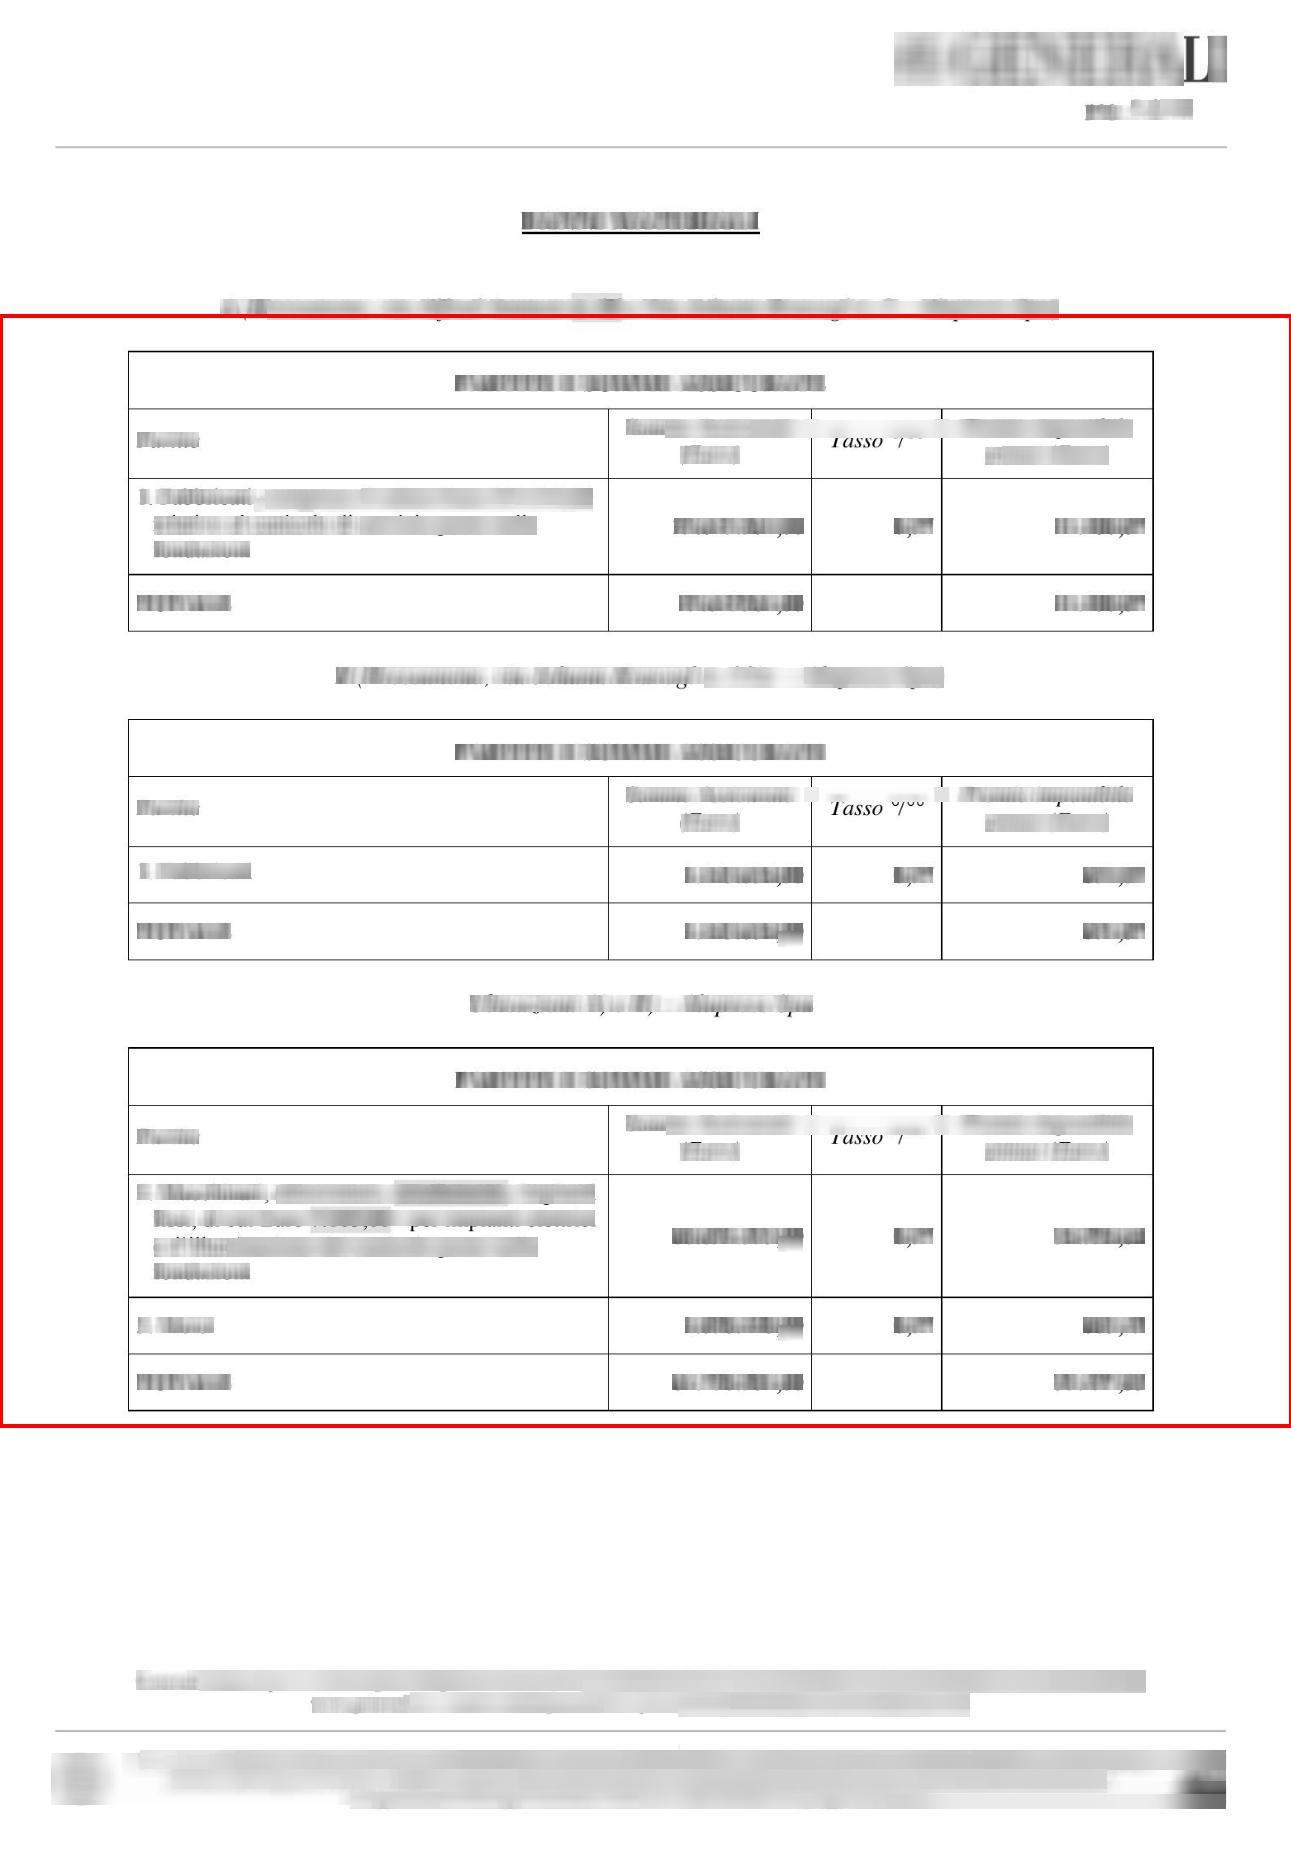
\includegraphics[width=1\columnwidth]{appendice/unite/test1_merged_0_6_adam_4}  
    \end{minipage}  
    \caption{Test 1, configurazione 3}
\end{figure}%  
Configurazione:
\begin{multicols}{2}
    \begin{lstlisting}
image_resizer {
  fixes_shape_resizer {
    width: 400
    heigth: 400
  }
}
first_stage_box_predictor {
  l2_regularizer {
    weight: 0.04
}
first_stage_nms_iou_threshold: 0.7
second_stage_box_predictor {
  l2_regularizer {
    weight: 0.004
  }
}
second_stage_post_processing {
  iou_threshold: 0.6
}
optimizer {
  adam_optimizer: {
    learning_rate: {
      exponential_decay_learning_rate {
        initial_learning_rate: 0.0001
          decay_steps: 450
          decay_factor: 0.9
        }
      }
    ...
  use_moving_average: false
}
    \end{lstlisting}
\end{multicols}

%============================================================================================
\newpage
\begin{figure}[H]  
    \begin{minipage}{.5\columnwidth}  
        \centering  
        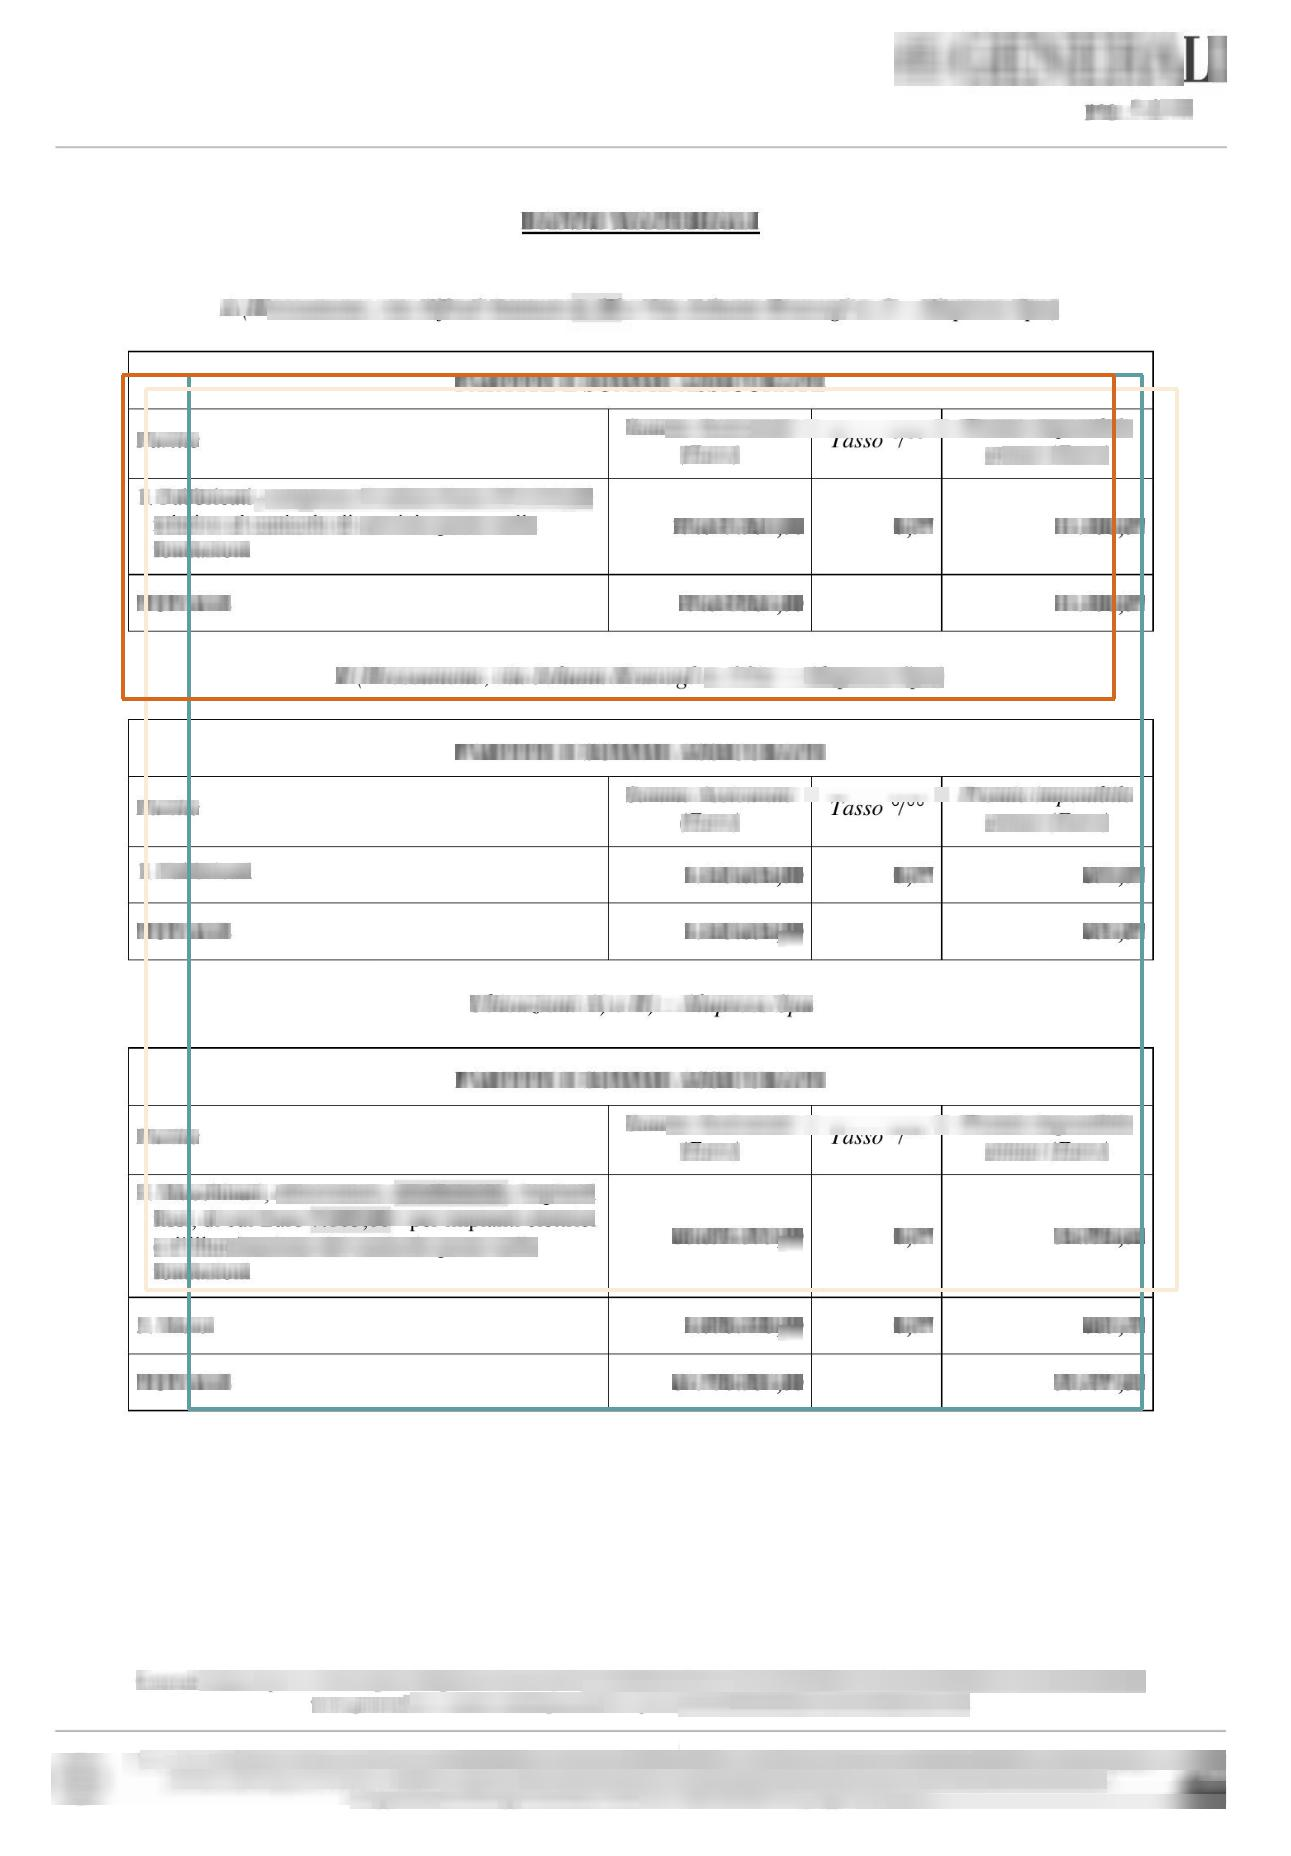
\includegraphics[width=1\columnwidth]{appendice/filtrate/test1_filtered_0_6_momentum_1}  
    \end{minipage}%  
    \begin{minipage}{0.5\columnwidth}  
        \centering  
        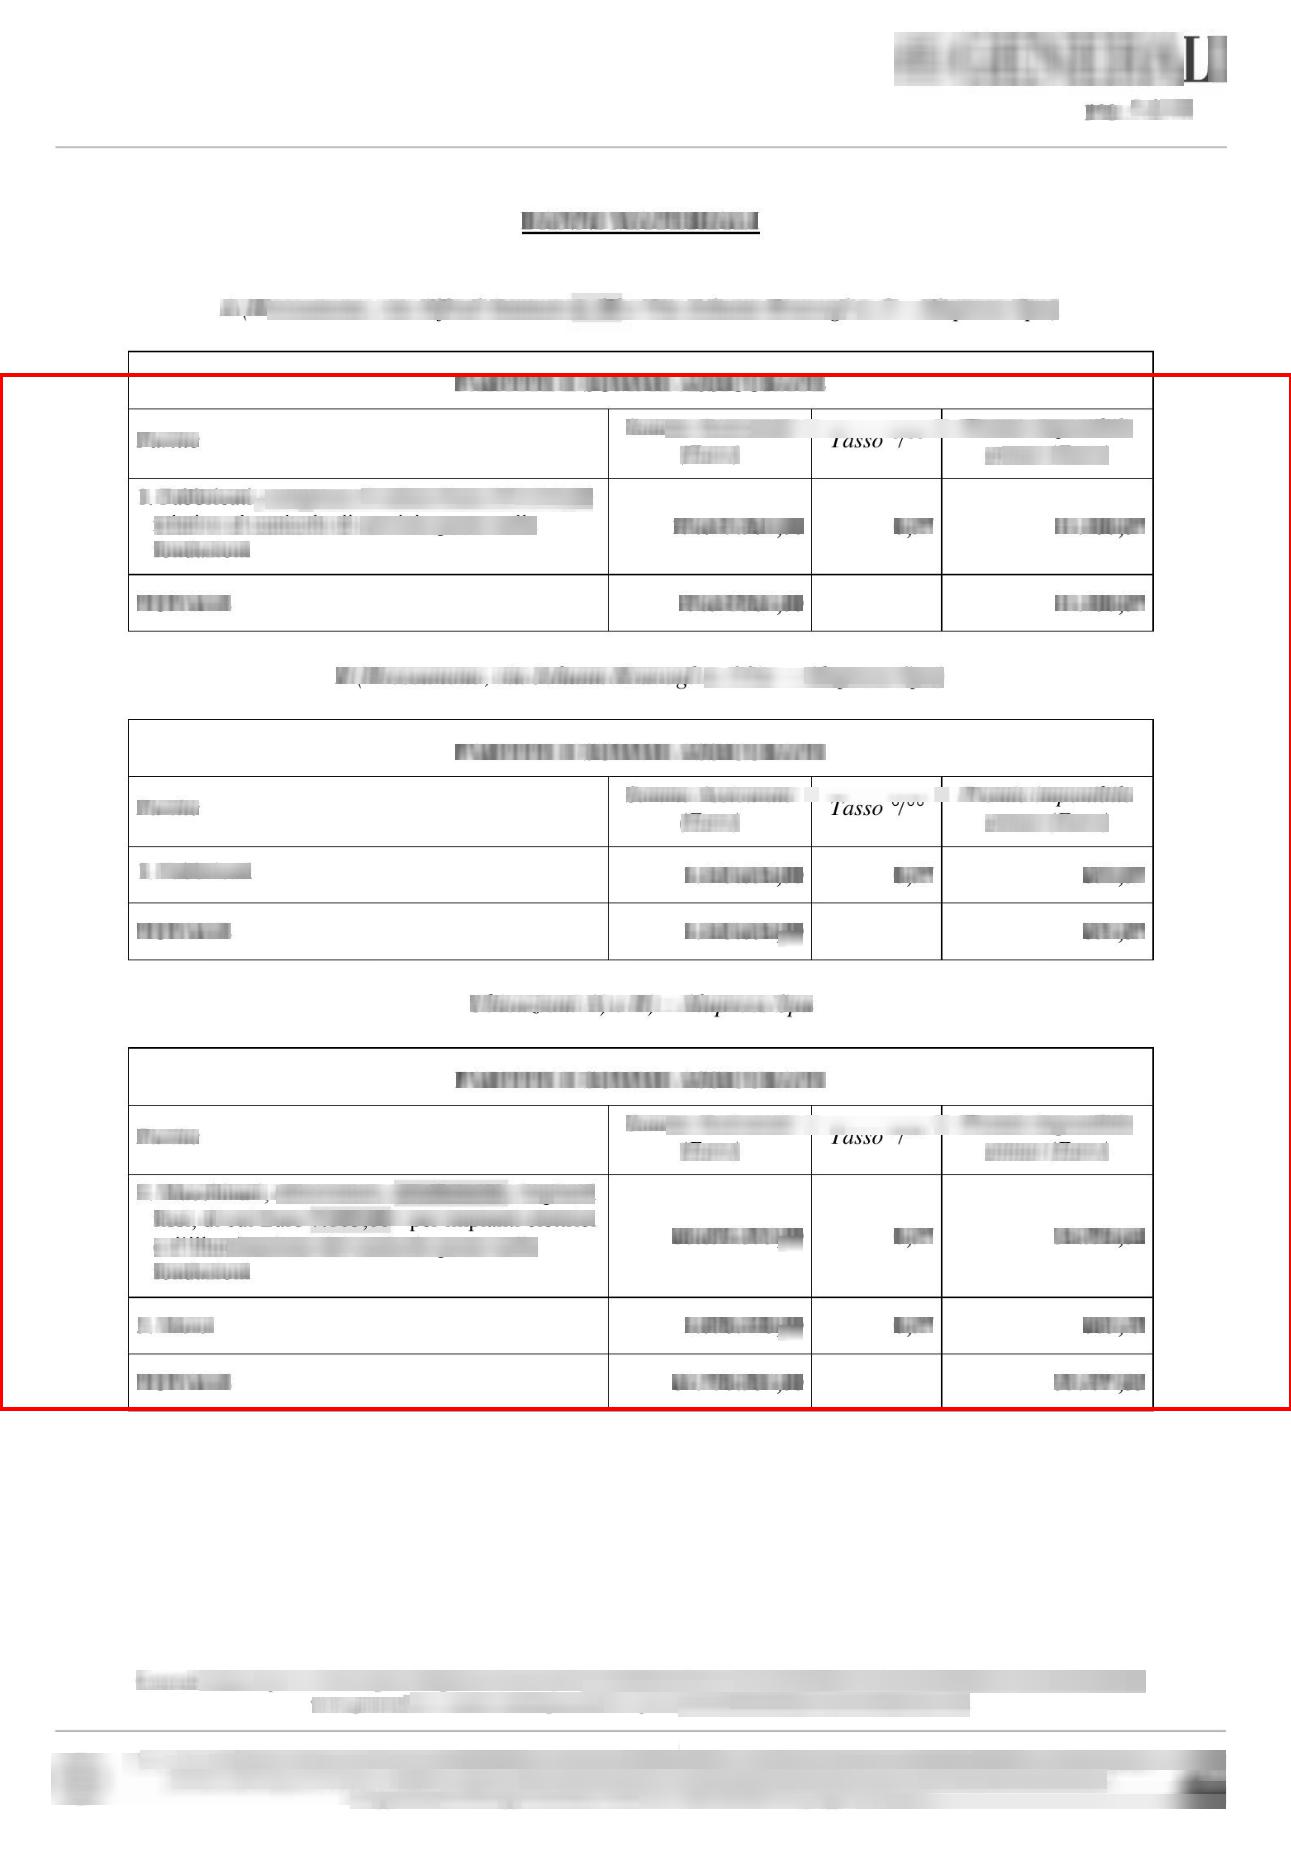
\includegraphics[width=1\columnwidth]{appendice/unite/test1_merged_0_6_momentum_1}  
    \end{minipage}  
    \caption{Test 1, configurazione 4}
\end{figure}%  
Configurazione:
\begin{multicols}{2}
    \begin{lstlisting}
image_resizer {
  fixes_shape_resizer {
    width: 400
    heigth: 400
  }
}
first_stage_box_predictor {
  l2_regularizer {
    weight: 0.00001
}
first_stage_nms_iou_threshold: 0.7
second_stage_box_predictor {
  l2_regularizer {
    weight: 0.00004
  }
}
second_stage_post_processing {
  iou_threshold: 0.6
}
optimizer {
  adam_optimizer: {
    learning_rate: {
      manual_step_learning_rate {
        initial_learning_rate: 0.0008
        schedule {
          step: 4500
          learning_rate: .0008
        }
        schedule {
          step: 7000
          learning_rate: .0004
        }
        schedule {
          step: 10000
          learning_rate: .00008
        }
    ...
    }
    momentum_optimizer_value: 0.9
  }
  use_moving_average: false
}
    \end{lstlisting}
\end{multicols}
%============================================================================================

\newpage
\begin{figure}[H]  
    \begin{minipage}{.5\columnwidth}  
        \centering  
        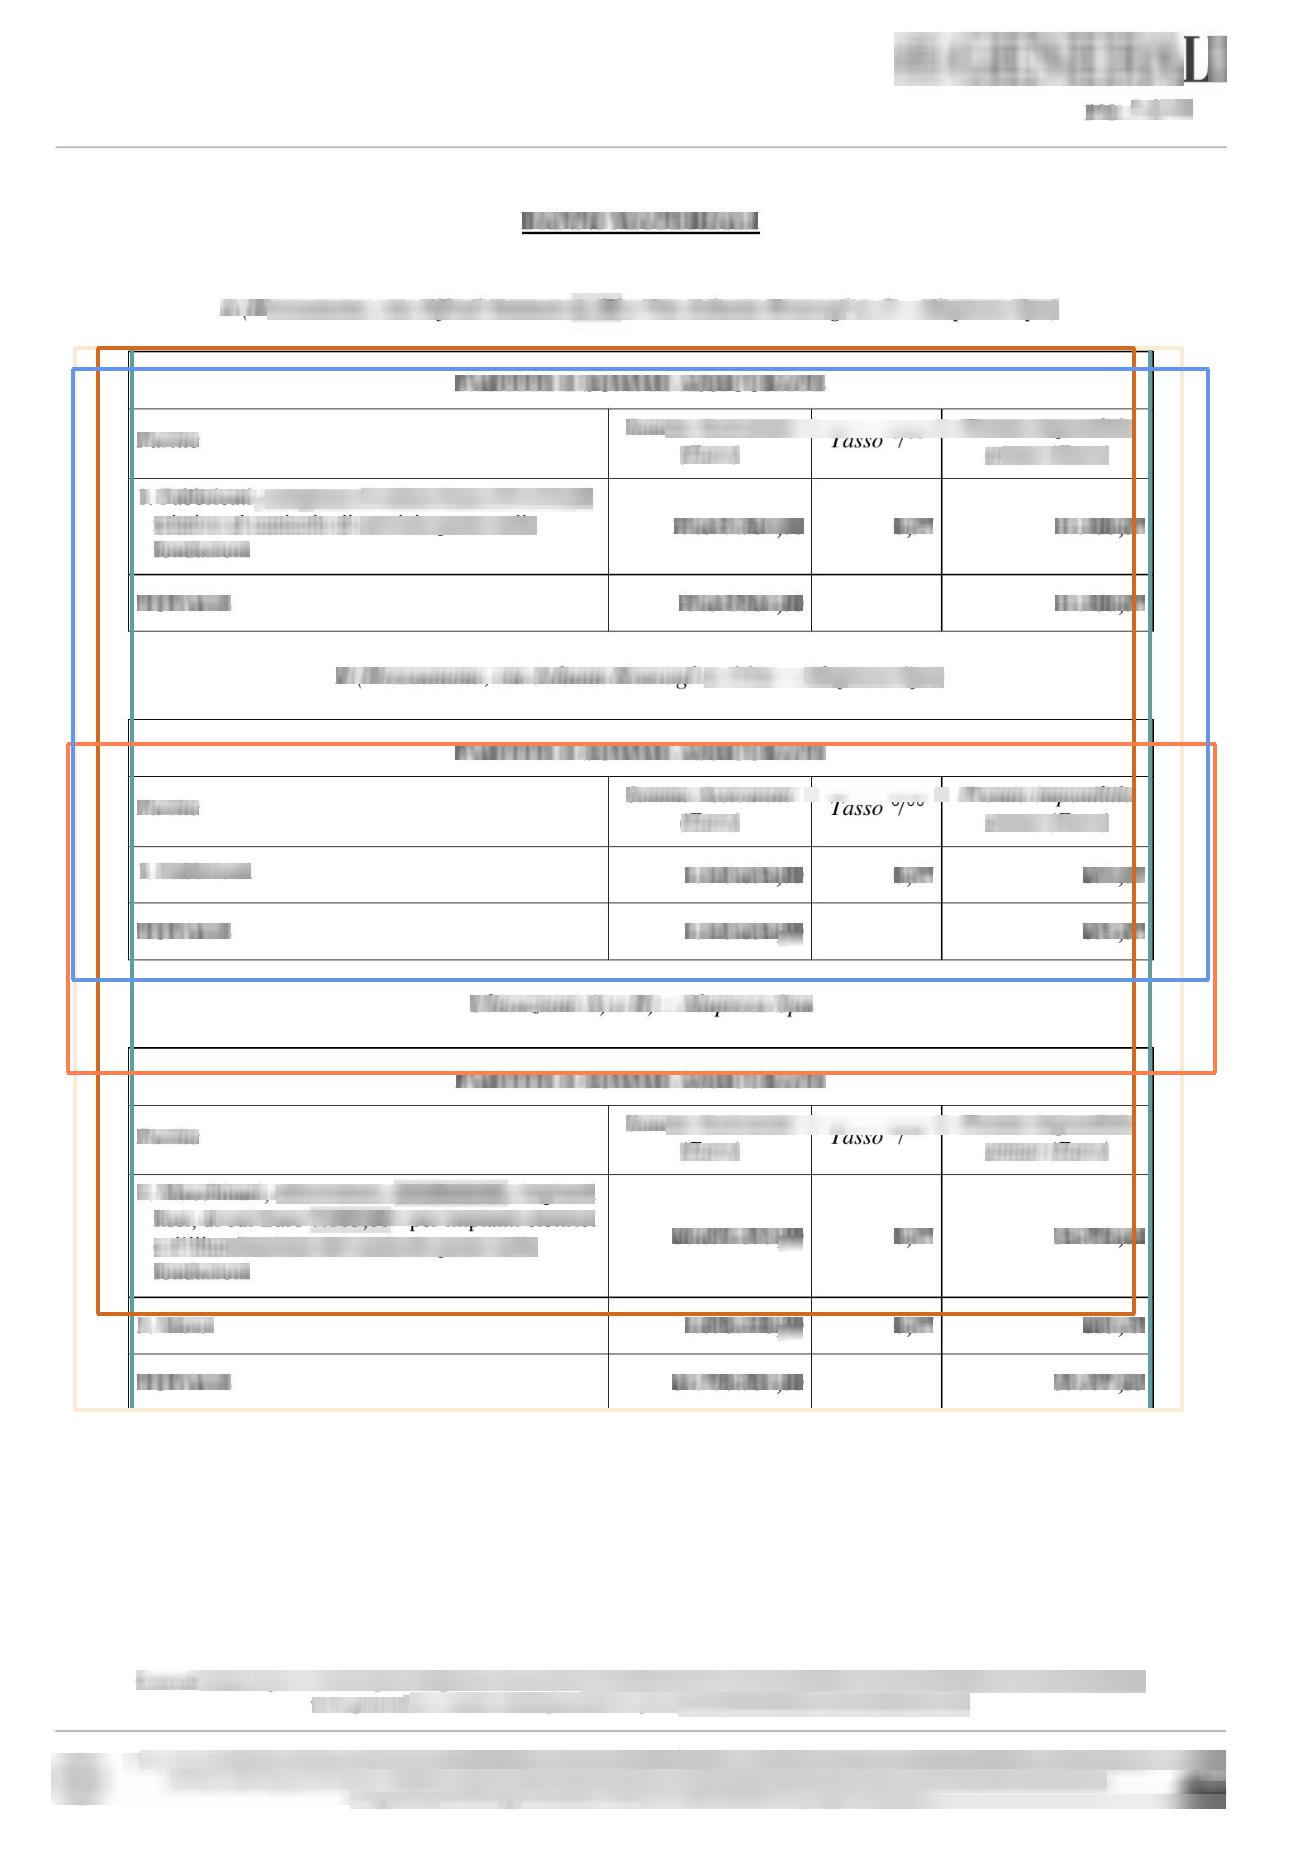
\includegraphics[width=1\columnwidth]{appendice/filtrate/test1_filtered_0_6_momentum_10k_jpg}  
    \end{minipage}%  
    \begin{minipage}{0.5\columnwidth}  
        \centering  
        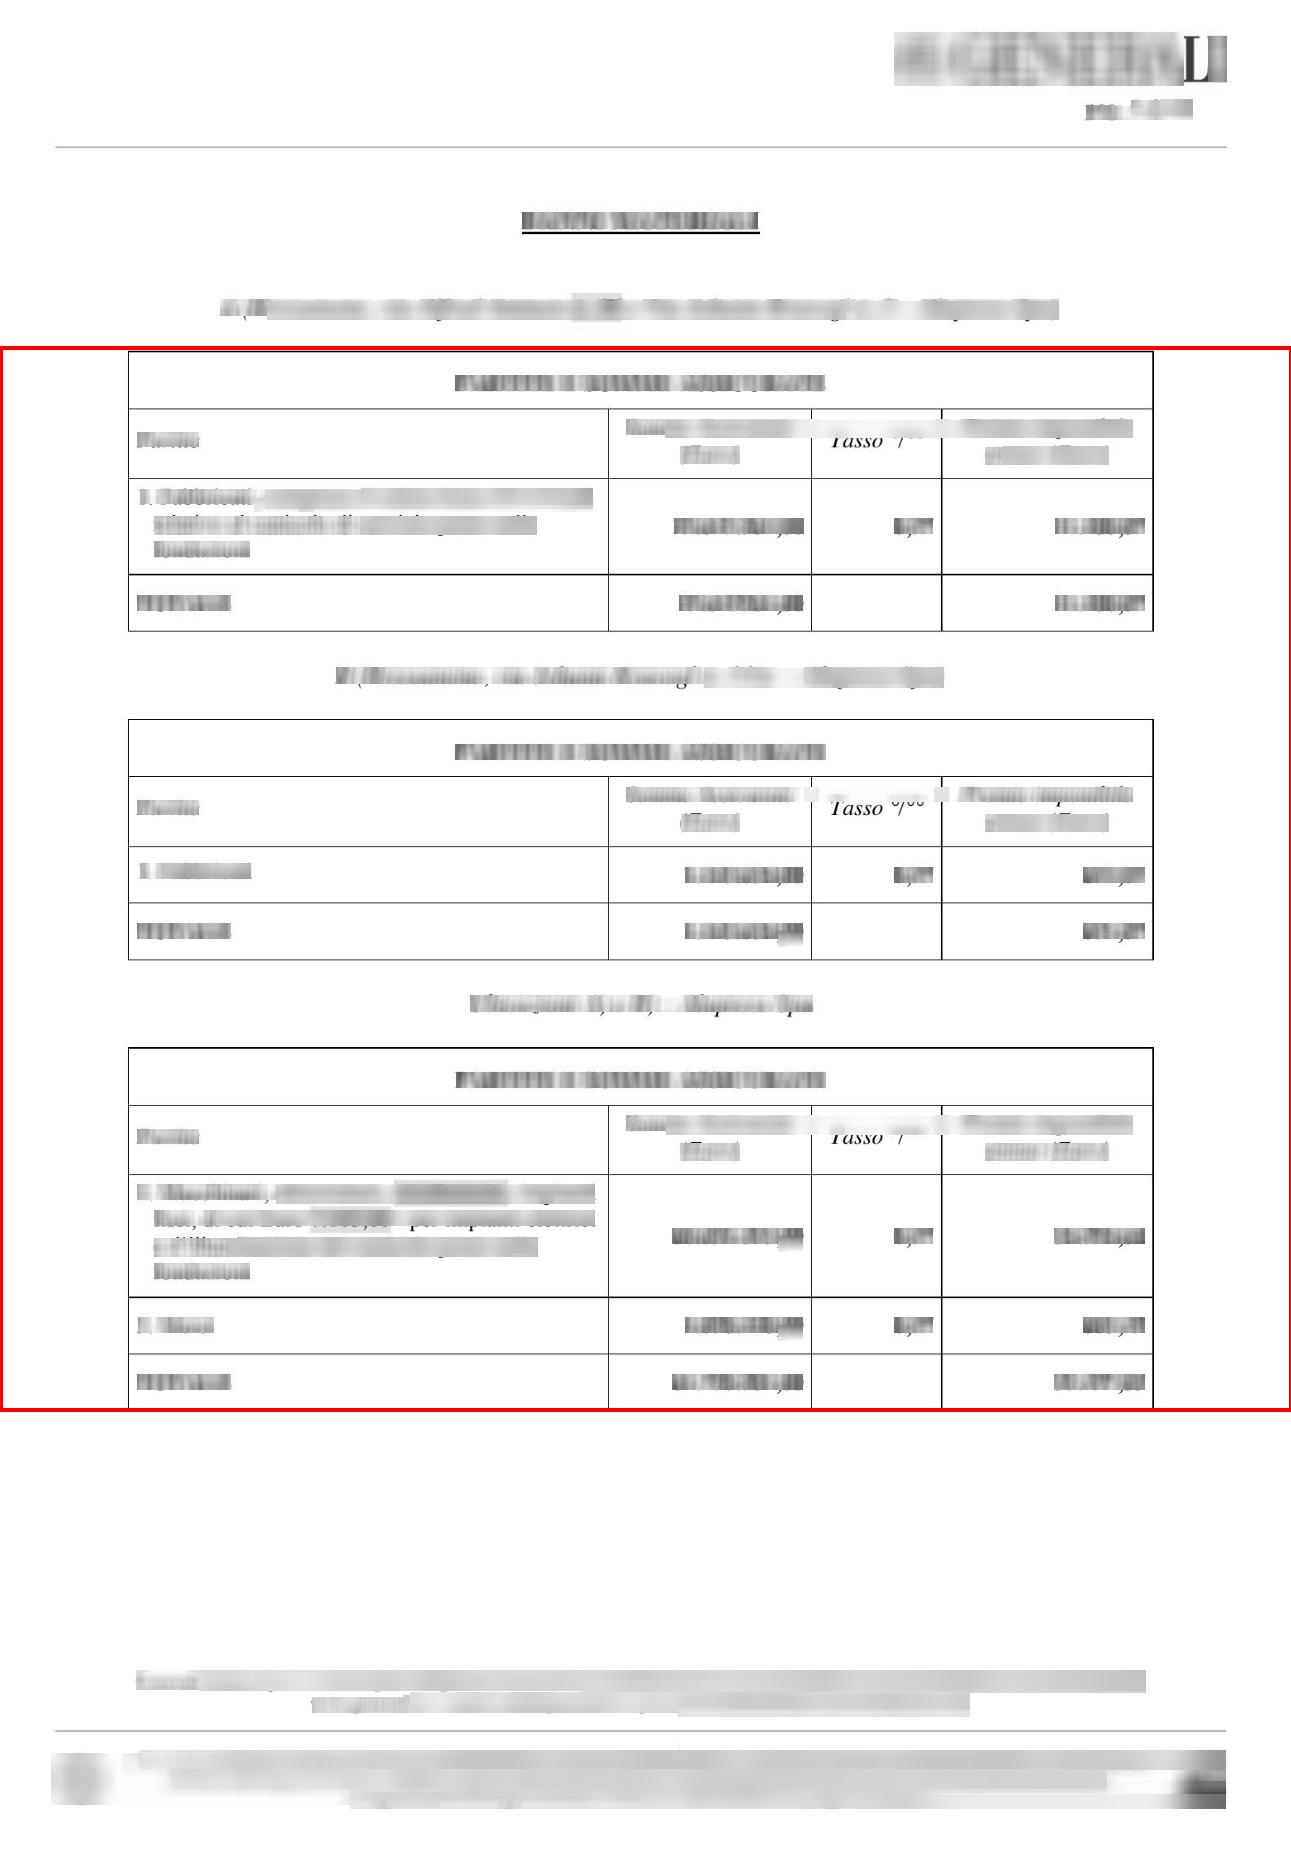
\includegraphics[width=1\columnwidth]{appendice/unite/test1_merged_0_6_momentum_10k_jpg}  
    \end{minipage}  
    \caption{Test 1, configurazione 5}
\end{figure}%  
Configurazione:
\begin{multicols}{2}
    \begin{lstlisting}
image_resizer {
  fixes_shape_resizer {
    width: 400
    heigth: 400
  }
}
first_stage_box_predictor {
  l2_regularizer {
    weight: 0.004
}
first_stage_nms_iou_threshold: 0.7
second_stage_box_predictor {
  l2_regularizer {
    weight: 0.004
  }
}
second_stage_post_processing {
  iou_threshold: 0.6
}
optimizer {
  adam_optimizer: {
    learning_rate: {
      manual_step_learning_rate {
        initial_learning_rate: 0.0004
        schedule {
          step: 4500
          learning_rate: .0002
        }
        schedule {
          step: 7000
          learning_rate: .00002
        }
        schedule {
          step: 10000
          learning_rate: .000002
        }
    ...
    }
    momentum_optimizer_value: 0.9
  }
  use_moving_average: false
}
    \end{lstlisting}
\end{multicols}
%============================================================================================

\newpage
\begin{figure}[H]  
    \begin{minipage}{.5\columnwidth}  
        \centering  
        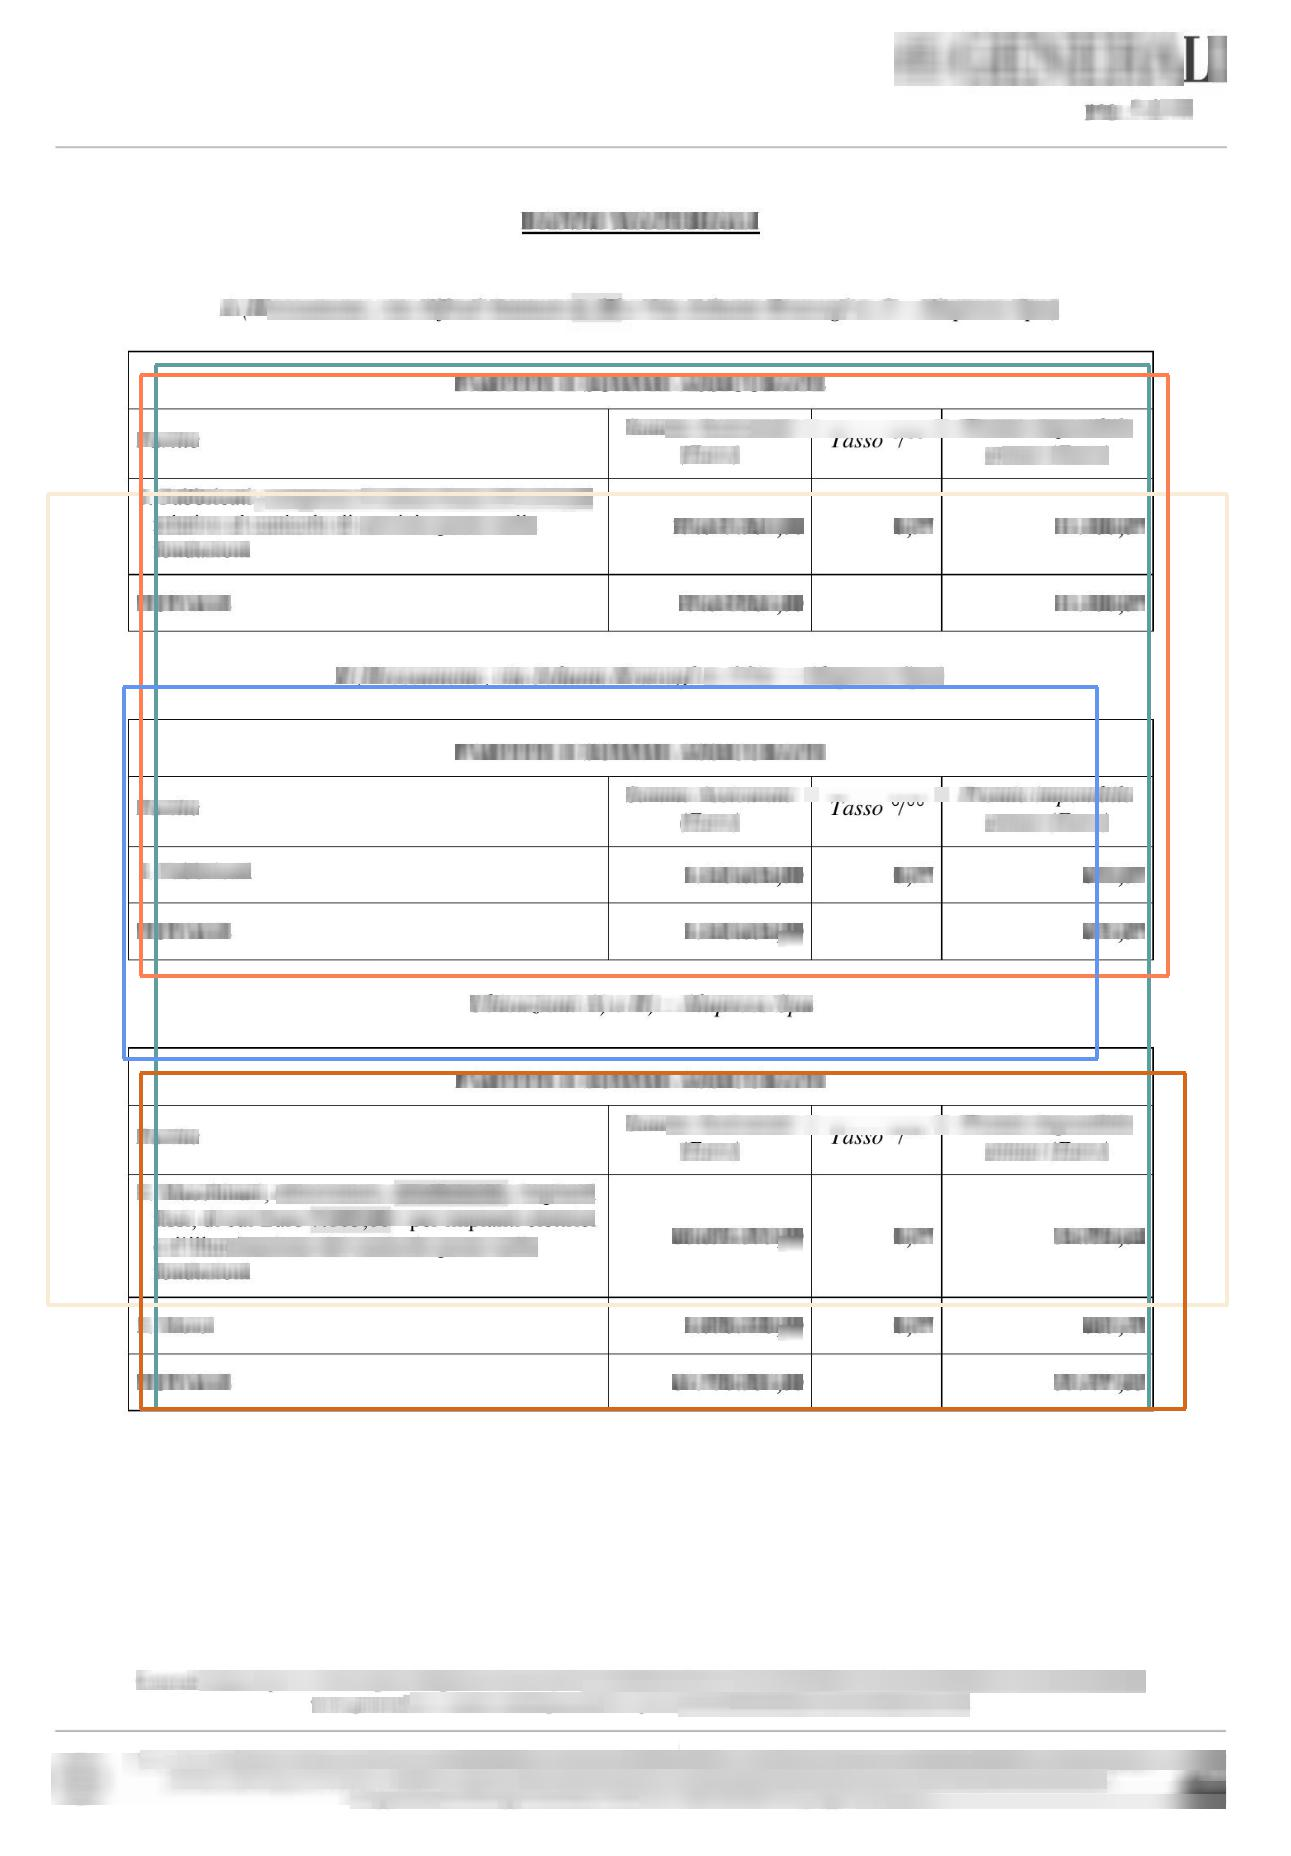
\includegraphics[width=1\columnwidth]{appendice/filtrate/test1_filtered_0_6_momentum_optimizer_1batch}  
    \end{minipage}%  
    \begin{minipage}{0.5\columnwidth}  
        \centering  
        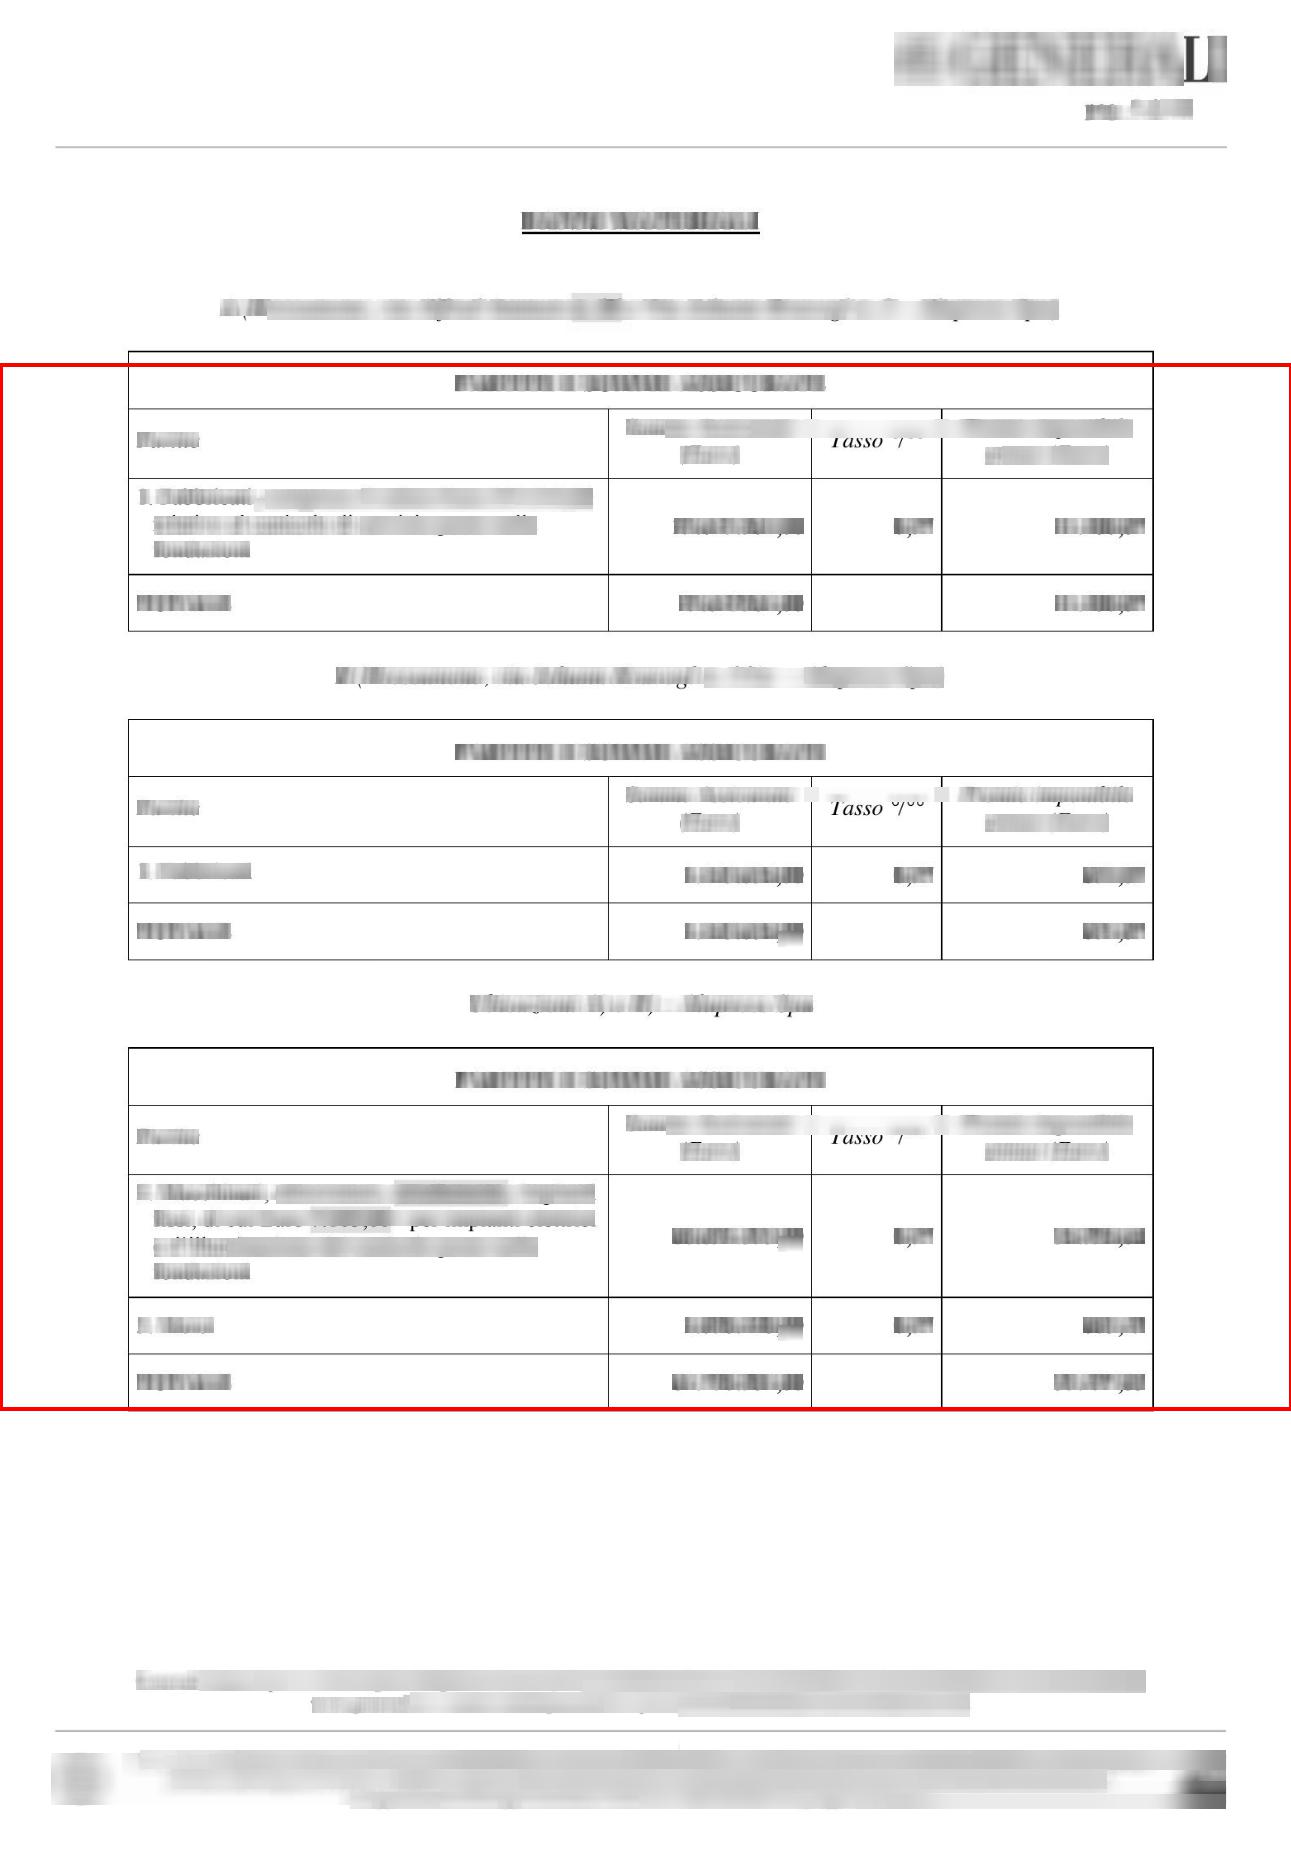
\includegraphics[width=1\columnwidth]{appendice/unite/test1_merged_0_6_momentum_optimizer_1batch}  
    \end{minipage}  
    \caption{Test 1, configurazione 6}
\end{figure}%  
Configurazione:
\begin{multicols}{2}
    \begin{lstlisting}
image_resizer {
  fixes_shape_resizer {
    width: 400
    heigth: 400
  }
}
first_stage_box_predictor {
  l2_regularizer {
    weight: 0.04
}
first_stage_nms_iou_threshold: 0.7
second_stage_box_predictor {
  l2_regularizer {
    weight: 0.004
  }
}
second_stage_post_processing {
  iou_threshold: 0.6
}
batch_size: 1
optimizer {
  adam_optimizer: {
    learning_rate: {
      manual_step_learning_rate {
        initial_learning_rate: 0.0004
        schedule {
          step: 4500
          learning_rate: .0002
        }
        schedule {
          step: 7000
          learning_rate: .00002
        }
        schedule {
          step: 10000
          learning_rate: .000002
        }
    ...
    }
    momentum_optimizer_value: 0.9
  }
  use_moving_average: false
}
    \end{lstlisting}
\end{multicols}
%============================================================================================
\newpage
\subsection{Test 2}
\begin{figure}[!ht] 
    \centering
    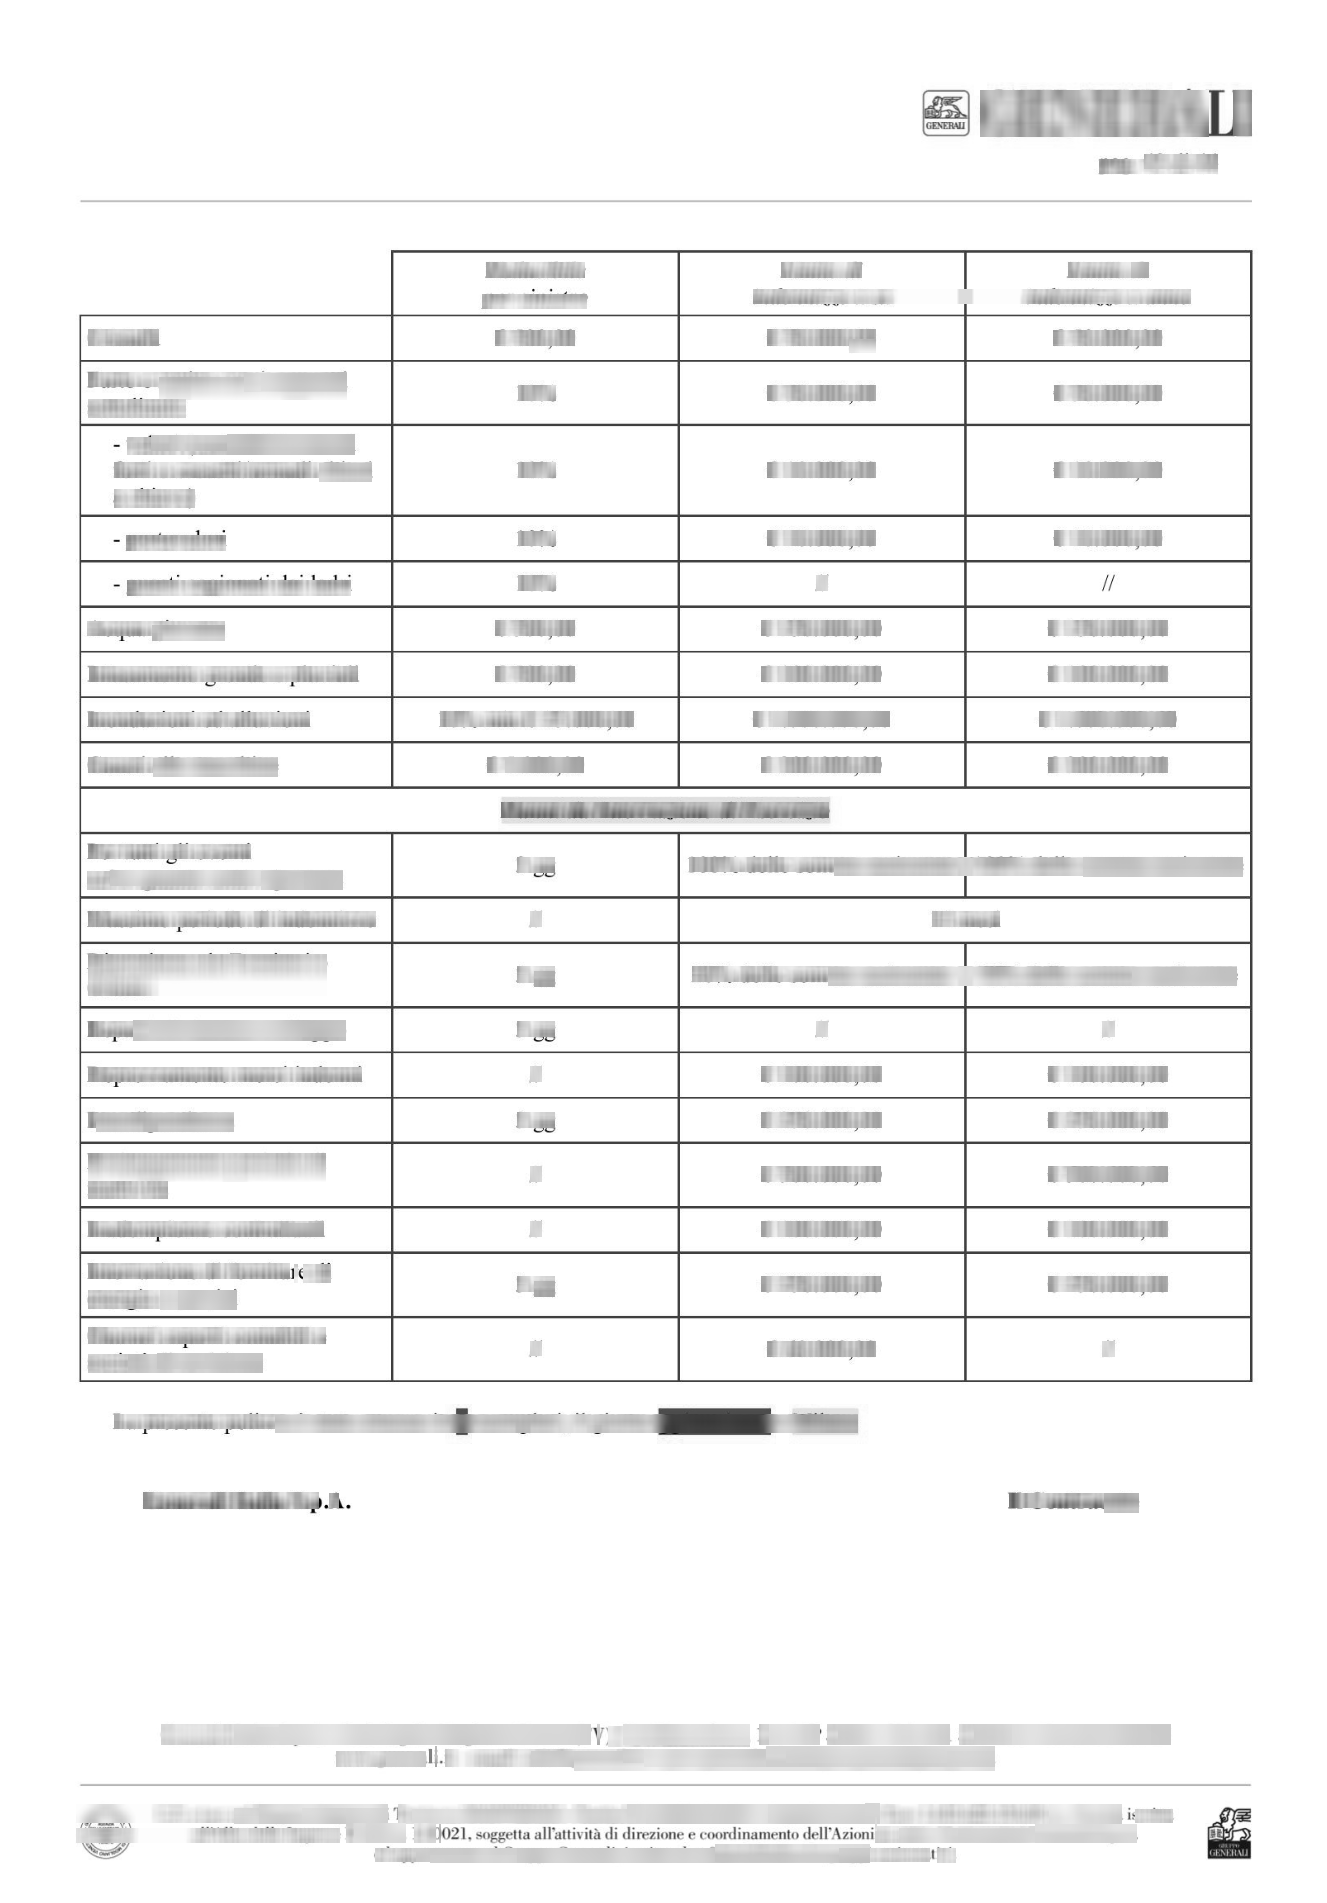
\includegraphics[width=1\columnwidth]{appendice/test2} 
    \caption{Test 2}
    \label{img:test-1}
\end{figure} 
\newpage

%============================================================================================


\begin{figure}[H]  
    \begin{minipage}{.5\columnwidth}  
        \centering  
        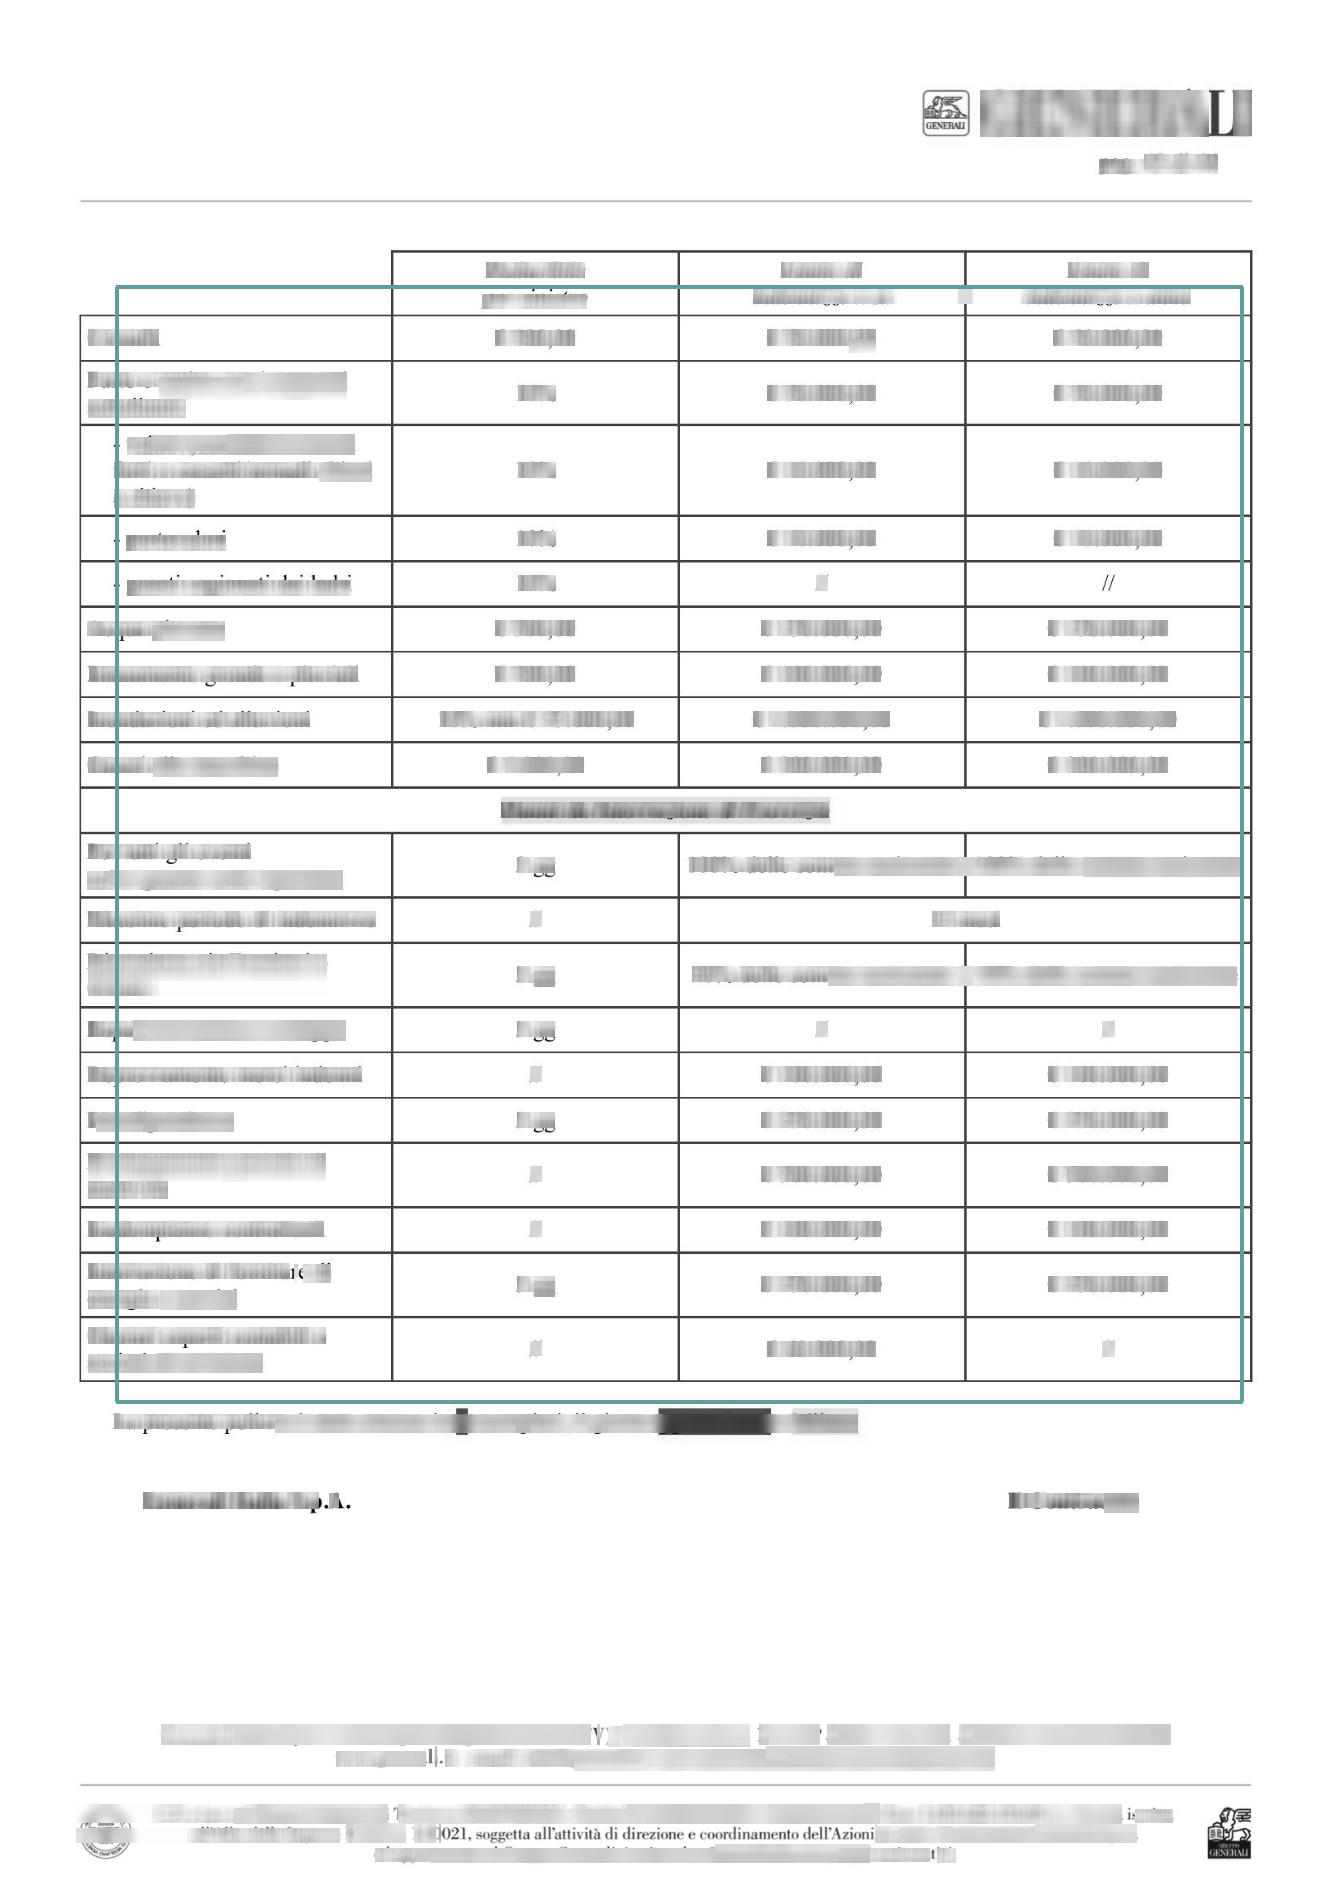
\includegraphics[width=1\columnwidth]{appendice/filtrate/test2_filtered_0_6_adam_1}  
    \end{minipage}%  
    \begin{minipage}{0.5\columnwidth}  
        \centering  
        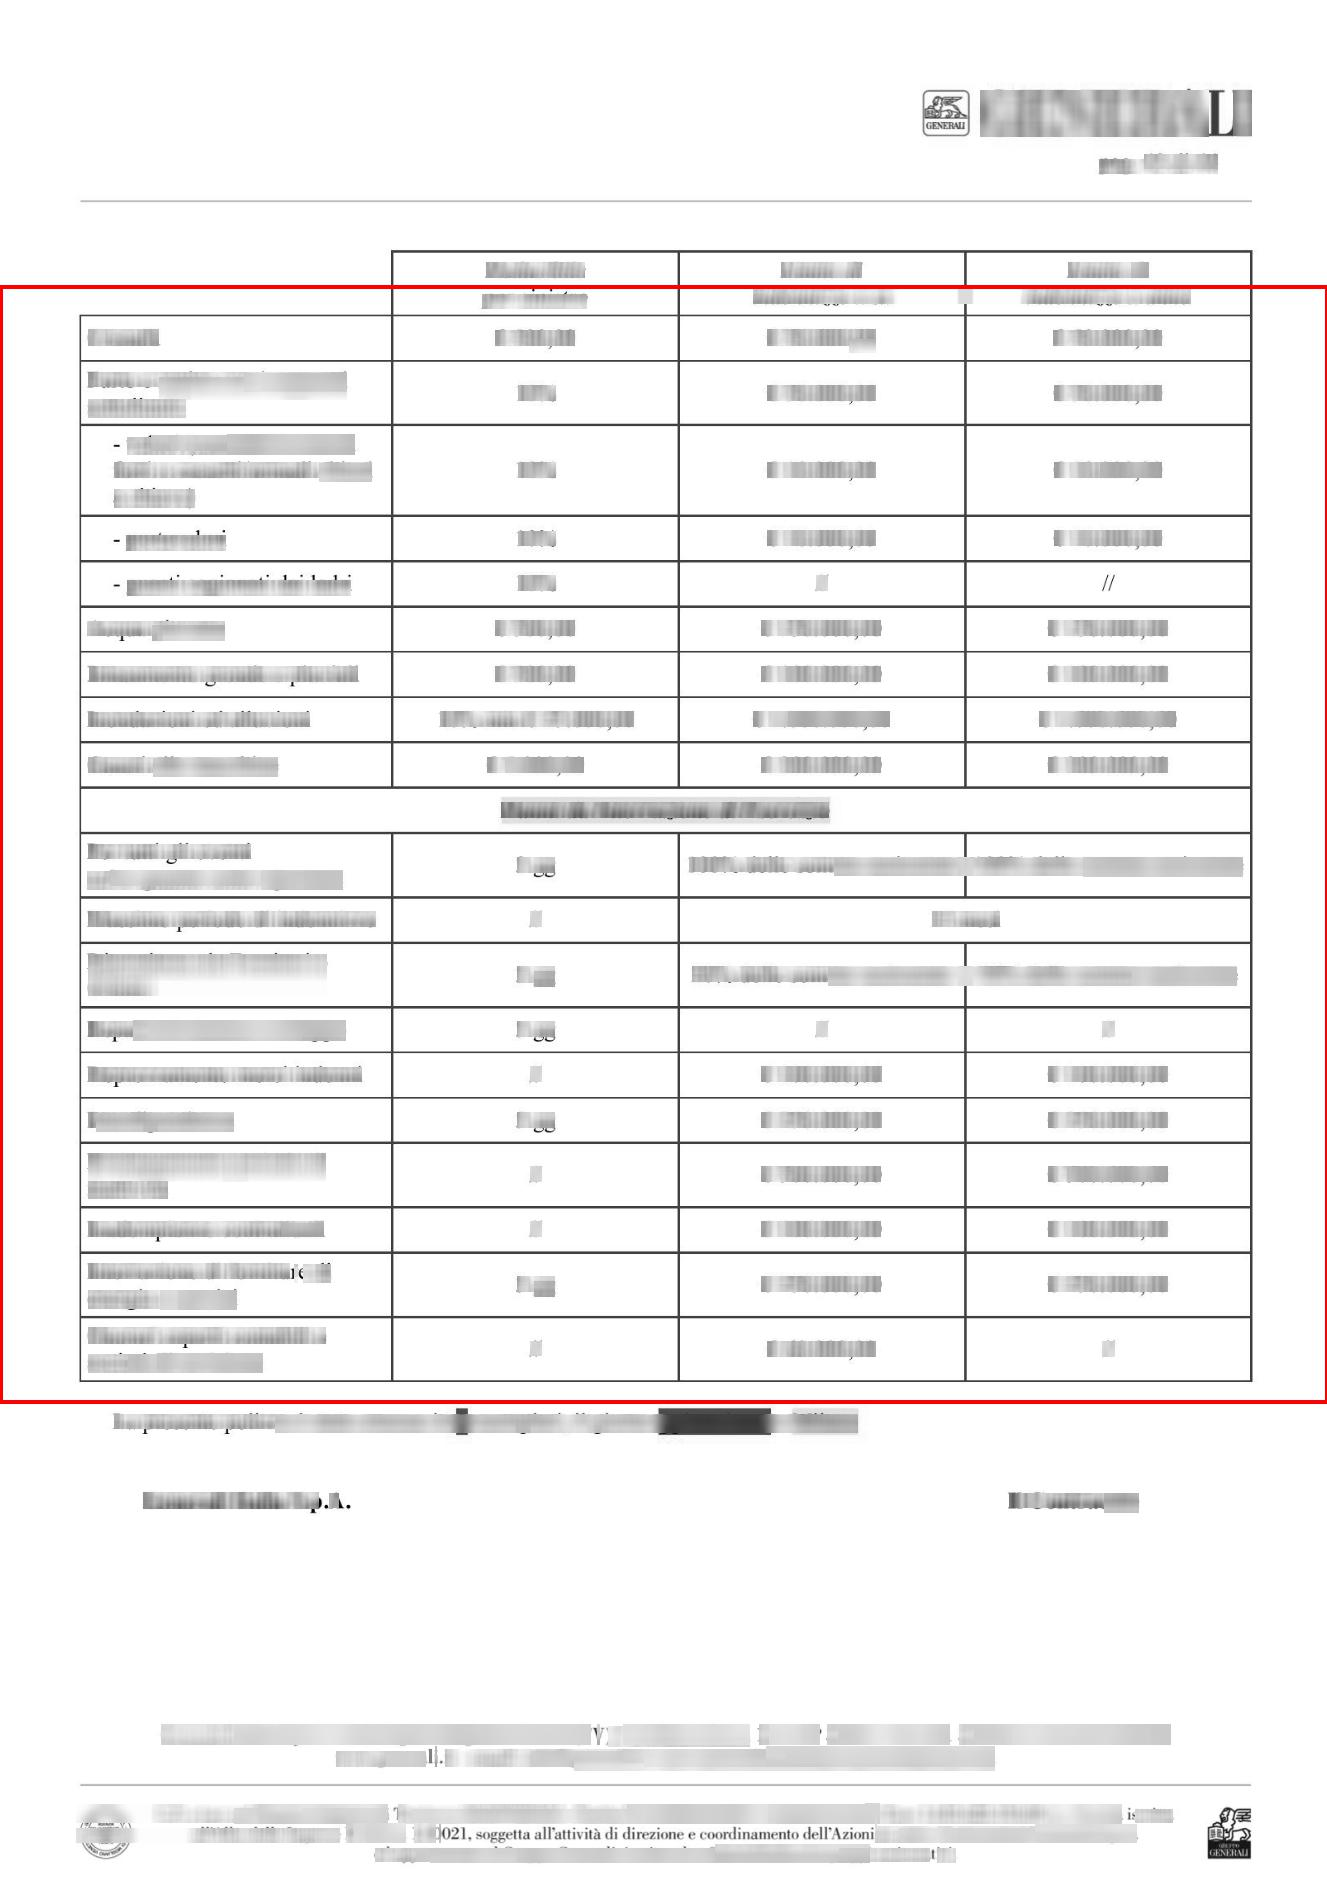
\includegraphics[width=1\columnwidth]{appendice/unite/test2_merged_0_6_adam_1}  
    \end{minipage}  
    \caption{Test 2, configurazione 1}
\end{figure}%  
Configurazione:
\begin{multicols}{2}
    \begin{lstlisting}
image_resizer {
  fixes_shape_resizer {
    width: 400
    heigth: 400
  }
}
first_stage_box_predictor {
  l2_regularizer {
    weight: 0.008
}
first_stage_nms_iou_threshold: 0.7
second_stage_box_predictor {
  l2_regularizer {
    weight: 0.004
  }
}
second_stage_post_processing {
  iou_threshold: 0.6
}
optimizer {
  adam_optimizer: {
    learning_rate: {
      manual_step_learning_rate {
        initial_learning_rate: .00008
        schedule {
          step: 4500
          learning_rate: .00004
        }
        schedule {
          step: 7000
          learning_rate: .00002
        }
        schedule {
          step: 10000
          learning_rate: .000008
        }
    ...
    }
    momentum_optimizer_value: 0.9
  }
  use_moving_average: false
}
\end{lstlisting}
\end{multicols}

%============================================================================================
\newpage
\begin{figure}[H]  
    \begin{minipage}{.5\columnwidth}  
        \centering  
        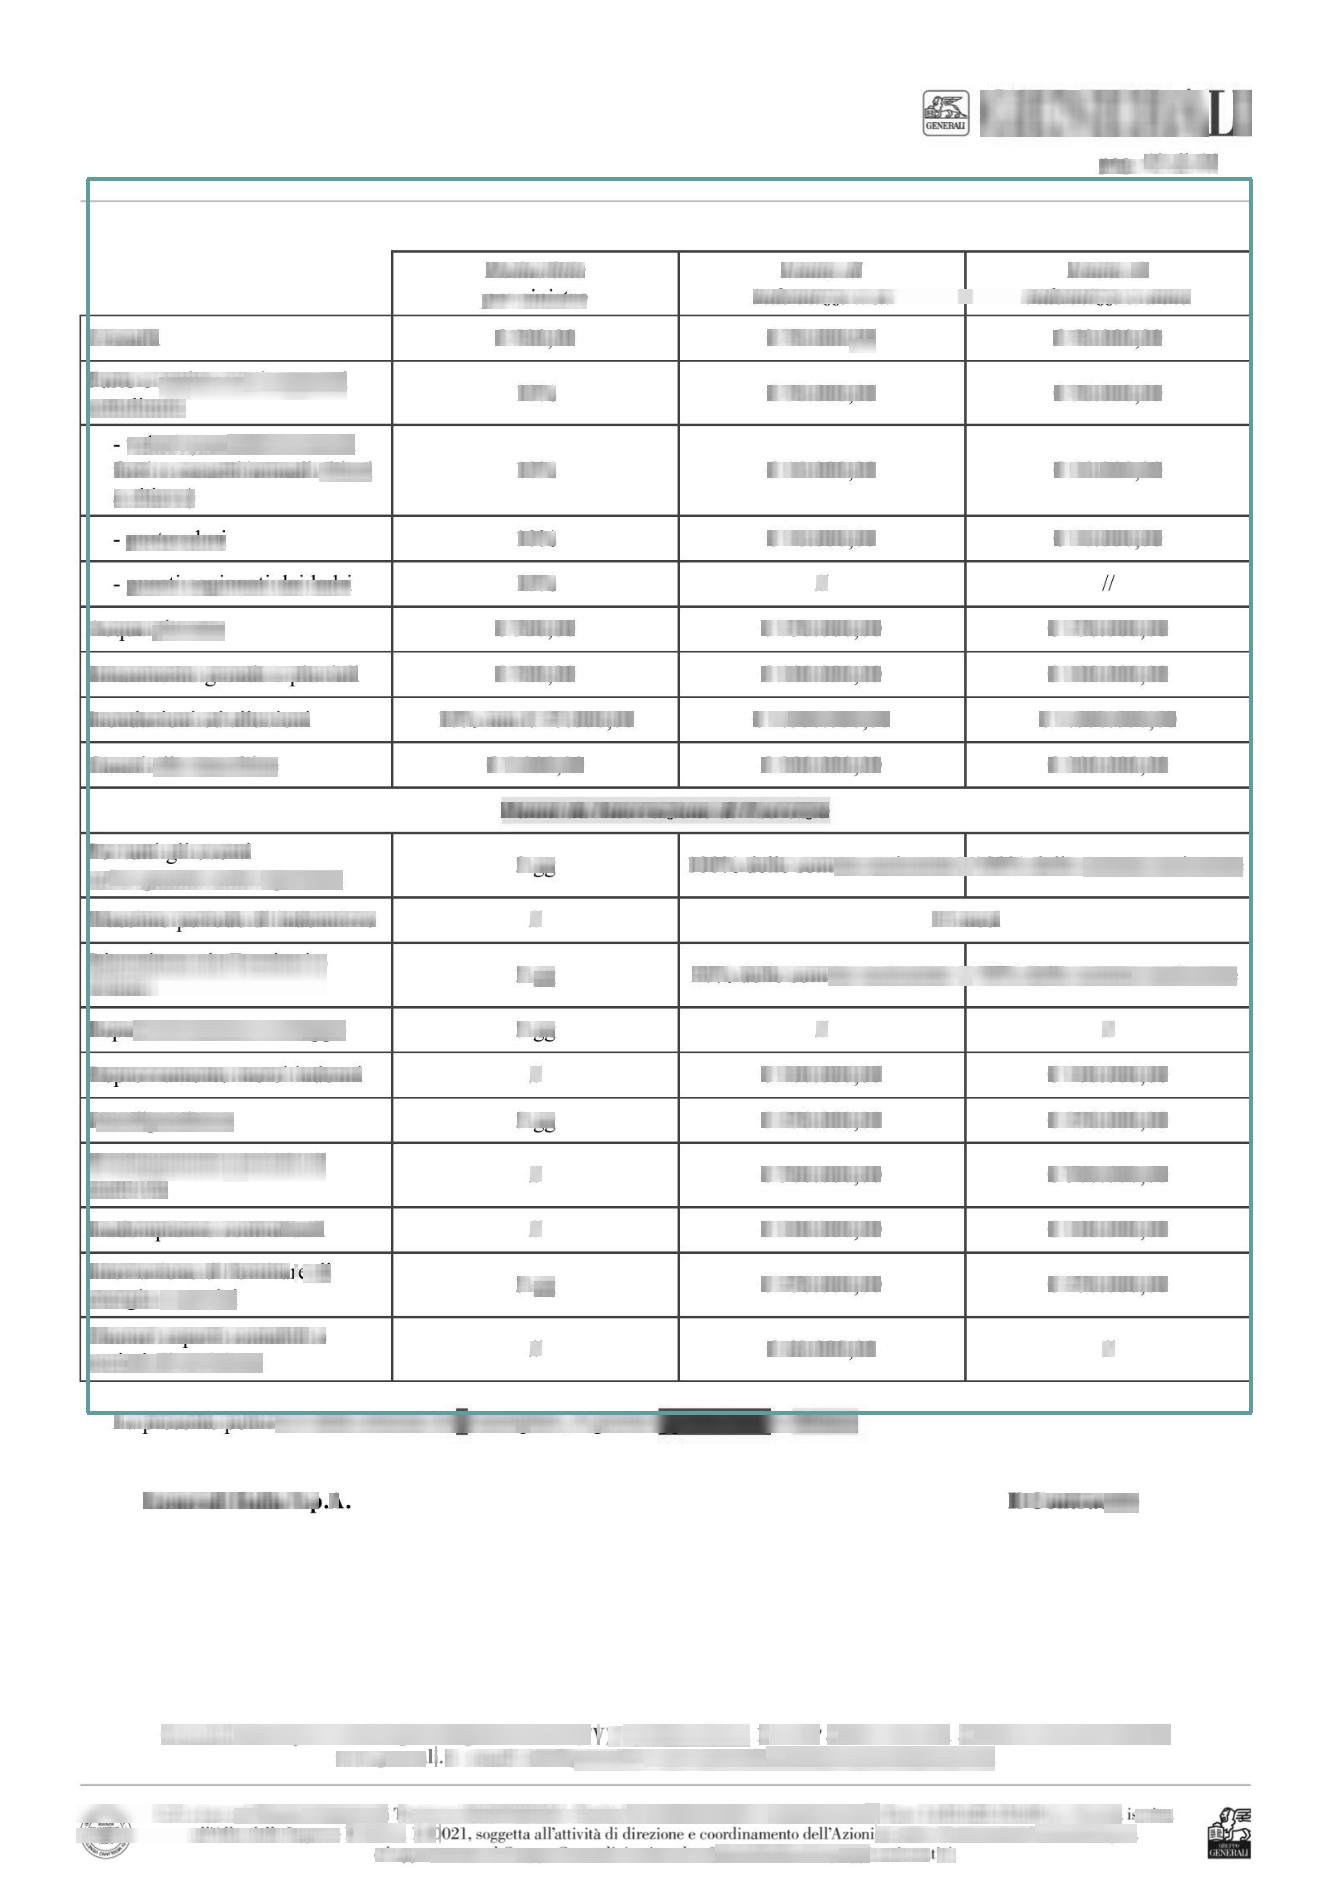
\includegraphics[width=1\columnwidth]{appendice/filtrate/test2_filtered_0_6_adam_3}  
    \end{minipage}%  
    \begin{minipage}{0.5\columnwidth}  
        \centering  
        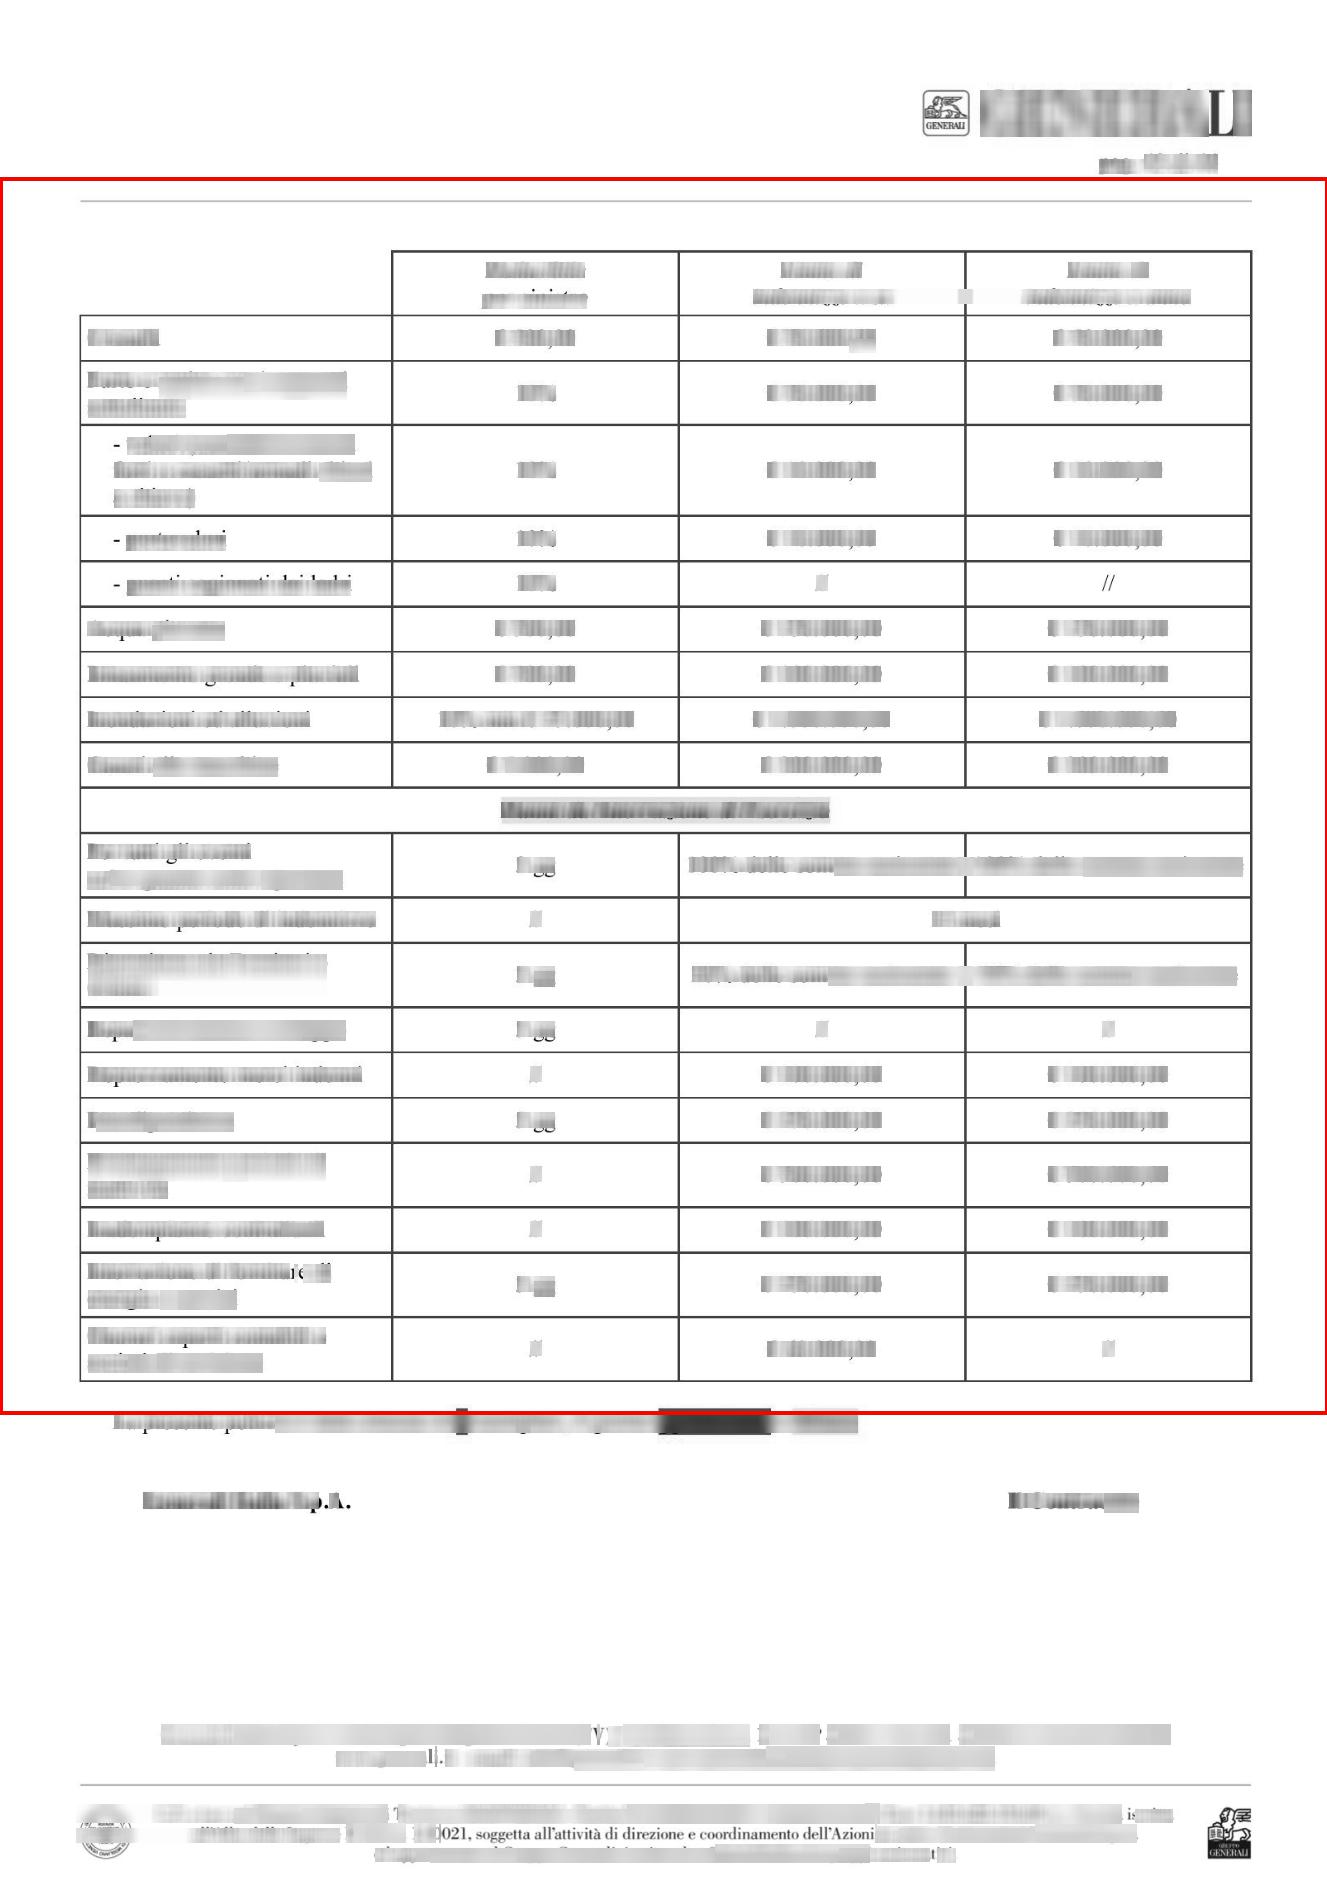
\includegraphics[width=1\columnwidth]{appendice/unite/test2_merged_0_6_adam_3}  
    \end{minipage}  
    \caption{Test 2, configurazione 2}
\end{figure}%  
Configurazione:
\begin{multicols}{2}
    \begin{lstlisting}
image_resizer {
  fixes_shape_resizer {
    width: 400
    heigth: 400
  }
}
first_stage_box_predictor {
  l2_regularizer {
    weight: 0.00001
}
first_stage_nms_iou_threshold: 0.7
second_stage_box_predictor {
  l2_regularizer {
    weight: 0.00004
  }
}
second_stage_post_processing {
  iou_threshold: 0.6
}
optimizer {
  adam_optimizer: {
    learning_rate: {
      exponential_decay_learning_rate {
        initial_learning_rate: 0.0001
          decay_steps: 600
          decay_factor: 0.95
        }
      }
    ...
  use_moving_average: false
}
    \end{lstlisting}
\end{multicols}

%============================================================================================
\newpage
\begin{figure}[H]  
    \begin{minipage}{.5\columnwidth}  
        \centering  
        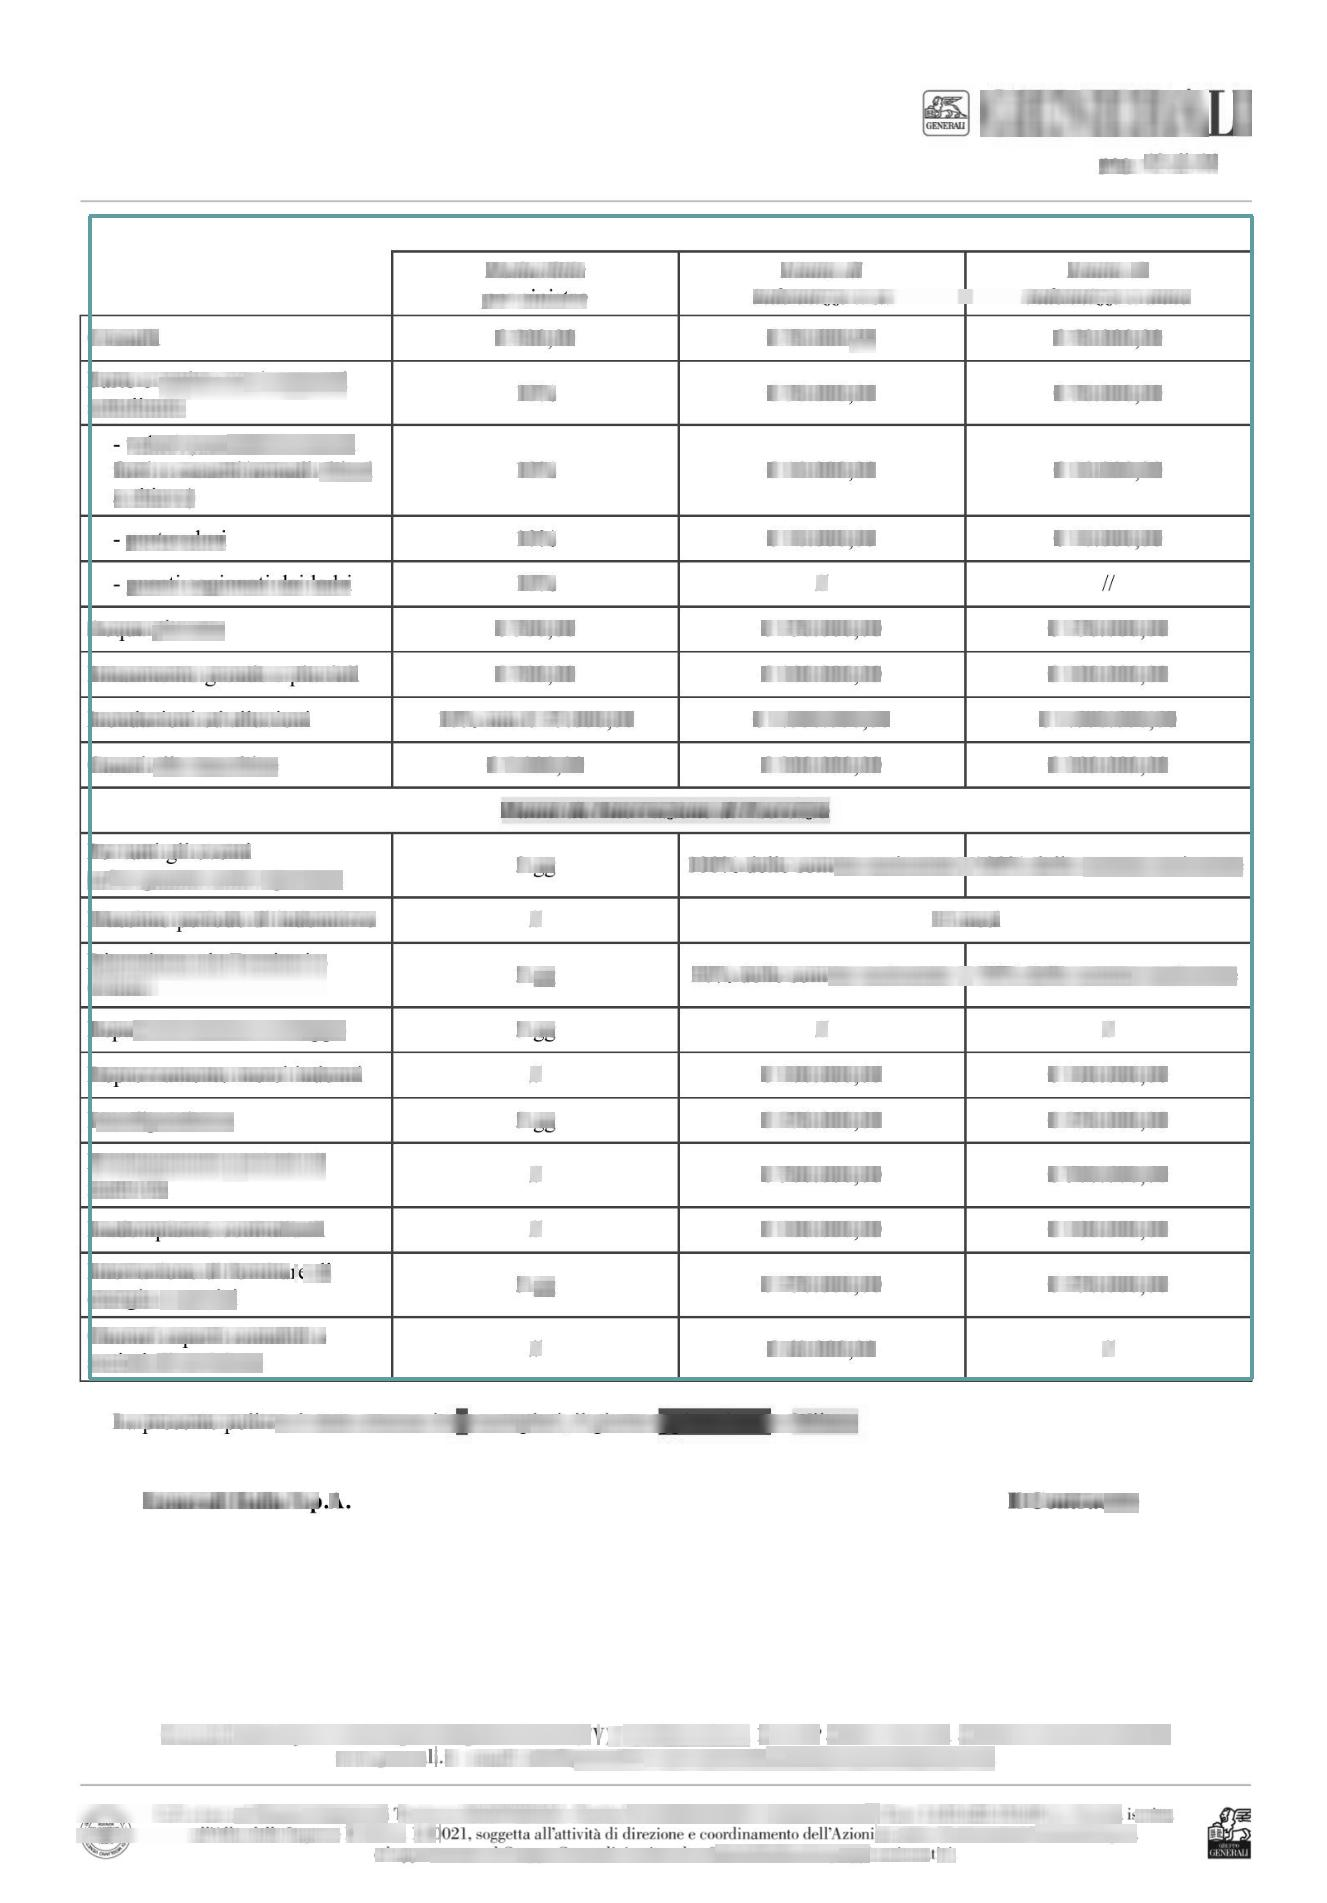
\includegraphics[width=1\columnwidth]{appendice/filtrate/test2_filtered_0_6_adam_4}  
    \end{minipage}%  
    \begin{minipage}{0.5\columnwidth}  
        \centering  
        \includegraphics[width=1\columnwidth]{appendice/unite/test2_merged_0_6_adam_4}  
    \end{minipage}  
    \caption{Test 2, configurazione 3}
\end{figure}%  
Configurazione:
\begin{multicols}{2}
    \begin{lstlisting}
image_resizer {
  fixes_shape_resizer {
    width: 400
    heigth: 400
  }
}
first_stage_box_predictor {
  l2_regularizer {
    weight: 0.04
}
first_stage_nms_iou_threshold: 0.7
second_stage_box_predictor {
  l2_regularizer {
    weight: 0.004
  }
}
second_stage_post_processing {
  iou_threshold: 0.6
}
optimizer {
  adam_optimizer: {
    learning_rate: {
      exponential_decay_learning_rate {
        initial_learning_rate: 0.0001
          decay_steps: 450
          decay_factor: 0.9
        }
      }
    ...
  use_moving_average: false
}
    \end{lstlisting}
\end{multicols}

%============================================================================================
\newpage
\begin{figure}[H]  
    \begin{minipage}{.5\columnwidth}  
        \centering  
        \includegraphics[width=1\columnwidth]{appendice/filtrate/test2_filtered_0_6_momentum_1}  
    \end{minipage}%  
    \begin{minipage}{0.5\columnwidth}  
        \centering  
        \includegraphics[width=1\columnwidth]{appendice/unite/test2_merged_0_6_momentum_1}  
    \end{minipage}  
    \caption{Test 2, configurazione 4}
\end{figure}%  
Configurazione:
\begin{multicols}{2}
    \begin{lstlisting}
image_resizer {
  fixes_shape_resizer {
    width: 400
    heigth: 400
  }
}
first_stage_box_predictor {
  l2_regularizer {
    weight: 0.00001
}
first_stage_nms_iou_threshold: 0.7
second_stage_box_predictor {
  l2_regularizer {
    weight: 0.00004
  }
}
second_stage_post_processing {
  iou_threshold: 0.6
}
optimizer {
  adam_optimizer: {
    learning_rate: {
      manual_step_learning_rate {
        initial_learning_rate: 0.0008
        schedule {
          step: 4500
          learning_rate: .0008
        }
        schedule {
          step: 7000
          learning_rate: .0004
        }
        schedule {
          step: 10000
          learning_rate: .00008
        }
    ...
    }
    momentum_optimizer_value: 0.9
  }
  use_moving_average: false
}
    \end{lstlisting}
\end{multicols}
%============================================================================================

\newpage
\begin{figure}[H]  
    \begin{minipage}{.5\columnwidth}  
        \centering  
        \includegraphics[width=1\columnwidth]{appendice/filtrate/test2_filtered_0_6_momentum_10k_jpg}  
    \end{minipage}%  
    \begin{minipage}{0.5\columnwidth}  
        \centering  
        \includegraphics[width=1\columnwidth]{appendice/unite/test2_merged_0_6_momentum_10k_jpg}  
    \end{minipage}  
    \caption{Test 2, configurazione 5}
\end{figure}%  
Configurazione:
\begin{multicols}{2}
    \begin{lstlisting}
image_resizer {
  fixes_shape_resizer {
    width: 400
    heigth: 400
  }
}
first_stage_box_predictor {
  l2_regularizer {
    weight: 0.004
}
first_stage_nms_iou_threshold: 0.7
second_stage_box_predictor {
  l2_regularizer {
    weight: 0.004
  }
}
second_stage_post_processing {
  iou_threshold: 0.6
}
optimizer {
  adam_optimizer: {
    learning_rate: {
      manual_step_learning_rate {
        initial_learning_rate: 0.0004
        schedule {
          step: 4500
          learning_rate: .0002
        }
        schedule {
          step: 7000
          learning_rate: .00002
        }
        schedule {
          step: 10000
          learning_rate: .000002
        }
    ...
    }
    momentum_optimizer_value: 0.9
  }
  use_moving_average: false
}
    \end{lstlisting}
\end{multicols}
%============================================================================================

\newpage
\begin{figure}[H]  
    \begin{minipage}{.5\columnwidth}  
        \centering  
        \includegraphics[width=1\columnwidth]{appendice/filtrate/test2_filtered_0_6_momentum_optimizer_1batch}  
    \end{minipage}%  
    \begin{minipage}{0.5\columnwidth}  
        \centering  
        \includegraphics[width=1\columnwidth]{appendice/unite/test2_merged_0_6_momentum_optimizer_1batch}  
    \end{minipage}  
    \caption{Test 2, configurazione 6}
\end{figure}%  
Configurazione:
\begin{multicols}{2}
    \begin{lstlisting}
image_resizer {
  fixes_shape_resizer {
    width: 400
    heigth: 400
  }
}
first_stage_box_predictor {
  l2_regularizer {
    weight: 0.04
}
first_stage_nms_iou_threshold: 0.7
second_stage_box_predictor {
  l2_regularizer {
    weight: 0.004
  }
}
second_stage_post_processing {
  iou_threshold: 0.6
}
batch_size: 1
optimizer {
  adam_optimizer: {
    learning_rate: {
      manual_step_learning_rate {
        initial_learning_rate: 0.0004
        schedule {
          step: 4500
          learning_rate: .0002
        }
        schedule {
          step: 7000
          learning_rate: .00002
        }
        schedule {
          step: 10000
          learning_rate: .000002
        }
    ...
    }
    momentum_optimizer_value: 0.9
  }
  use_moving_average: false
}
    \end{lstlisting}
\end{multicols}
%============================================================================================
\newpage
\subsection{Test 3}
\begin{figure}[!ht] 
    \centering
    \includegraphics[width=1\columnwidth]{appendice/test3} 
    \caption{Test 3}
    \label{img:test-1}
\end{figure} 
\newpage

%============================================================================================


\begin{figure}[H]  
    \begin{minipage}{.5\columnwidth}  
        \centering  
        \includegraphics[width=1\columnwidth]{appendice/filtrate/test3_filtered_0_6_adam_1}  
    \end{minipage}%  
    \begin{minipage}{0.5\columnwidth}  
        \centering  
        \includegraphics[width=1\columnwidth]{appendice/unite/test3_merged_0_6_adam_1}  
    \end{minipage}  
    \caption{Test 3, configurazione 1}
\end{figure}%  
Configurazione:
\begin{multicols}{2}
    \begin{lstlisting}
image_resizer {
  fixes_shape_resizer {
    width: 400
    heigth: 400
  }
}
first_stage_box_predictor {
  l2_regularizer {
    weight: 0.008
}
first_stage_nms_iou_threshold: 0.7
second_stage_box_predictor {
  l2_regularizer {
    weight: 0.004
  }
}
second_stage_post_processing {
  iou_threshold: 0.6
}
optimizer {
  adam_optimizer: {
    learning_rate: {
      manual_step_learning_rate {
        initial_learning_rate: .00008
        schedule {
          step: 4500
          learning_rate: .00004
        }
        schedule {
          step: 7000
          learning_rate: .00002
        }
        schedule {
          step: 10000
          learning_rate: .000008
        }
    ...
    }
    momentum_optimizer_value: 0.9
  }
  use_moving_average: false
}
\end{lstlisting}
\end{multicols}

%============================================================================================
\newpage
\begin{figure}[H]  
    \begin{minipage}{.5\columnwidth}  
        \centering  
        \includegraphics[width=1\columnwidth]{appendice/filtrate/test3_filtered_0_6_adam_3}  
    \end{minipage}%  
    \begin{minipage}{0.5\columnwidth}  
        \centering  
        \includegraphics[width=1\columnwidth]{appendice/unite/test3_merged_0_6_adam_3}  
    \end{minipage}  
    \caption{Test 3, configurazione 2}
\end{figure}%  
Configurazione:
\begin{multicols}{2}
    \begin{lstlisting}
image_resizer {
  fixes_shape_resizer {
    width: 400
    heigth: 400
  }
}
first_stage_box_predictor {
  l2_regularizer {
    weight: 0.00001
}
first_stage_nms_iou_threshold: 0.7
second_stage_box_predictor {
  l2_regularizer {
    weight: 0.00004
  }
}
second_stage_post_processing {
  iou_threshold: 0.6
}
optimizer {
  adam_optimizer: {
    learning_rate: {
      exponential_decay_learning_rate {
        initial_learning_rate: 0.0001
          decay_steps: 600
          decay_factor: 0.95
        }
      }
    ...
  use_moving_average: false
}
    \end{lstlisting}
\end{multicols}

%============================================================================================
\newpage
\begin{figure}[H]  
    \begin{minipage}{.5\columnwidth}  
        \centering  
        \includegraphics[width=1\columnwidth]{appendice/filtrate/test3_filtered_0_6_adam_4}  
    \end{minipage}%  
    \begin{minipage}{0.5\columnwidth}  
        \centering  
        \includegraphics[width=1\columnwidth]{appendice/unite/test3_merged_0_6_adam_4}  
    \end{minipage}  
    \caption{Test 3, configurazione 3}
\end{figure}%  
Configurazione:
\begin{multicols}{2}
    \begin{lstlisting}
image_resizer {
  fixes_shape_resizer {
    width: 400
    heigth: 400
  }
}
first_stage_box_predictor {
  l2_regularizer {
    weight: 0.04
}
first_stage_nms_iou_threshold: 0.7
second_stage_box_predictor {
  l2_regularizer {
    weight: 0.004
  }
}
second_stage_post_processing {
  iou_threshold: 0.6
}
optimizer {
  adam_optimizer: {
    learning_rate: {
      exponential_decay_learning_rate {
        initial_learning_rate: 0.0001
          decay_steps: 450
          decay_factor: 0.9
        }
      }
    ...
  use_moving_average: false
}
    \end{lstlisting}
\end{multicols}

%============================================================================================
\newpage
\begin{figure}[H]  
    \begin{minipage}{.5\columnwidth}  
        \centering  
        \includegraphics[width=1\columnwidth]{appendice/filtrate/test3_filtered_0_6_momentum_1}  
    \end{minipage}%  
    \begin{minipage}{0.5\columnwidth}  
        \centering  
        \includegraphics[width=1\columnwidth]{appendice/unite/test3_merged_0_6_momentum_1}  
    \end{minipage}  
    \caption{Test 3, configurazione 4}
\end{figure}%  
Configurazione:
\begin{multicols}{2}
    \begin{lstlisting}
image_resizer {
  fixes_shape_resizer {
    width: 400
    heigth: 400
  }
}
first_stage_box_predictor {
  l2_regularizer {
    weight: 0.00001
}
first_stage_nms_iou_threshold: 0.7
second_stage_box_predictor {
  l2_regularizer {
    weight: 0.00004
  }
}
second_stage_post_processing {
  iou_threshold: 0.6
}
optimizer {
  adam_optimizer: {
    learning_rate: {
      manual_step_learning_rate {
        initial_learning_rate: 0.0008
        schedule {
          step: 4500
          learning_rate: .0008
        }
        schedule {
          step: 7000
          learning_rate: .0004
        }
        schedule {
          step: 10000
          learning_rate: .00008
        }
    ...
    }
    momentum_optimizer_value: 0.9
  }
  use_moving_average: false
}
    \end{lstlisting}
\end{multicols}
%============================================================================================

\newpage
\begin{figure}[H]  
    \begin{minipage}{.5\columnwidth}  
        \centering  
        \includegraphics[width=1\columnwidth]{appendice/filtrate/test3_filtered_0_6_momentum_10k_jpg}  
    \end{minipage}%  
    \begin{minipage}{0.5\columnwidth}  
        \centering  
        \includegraphics[width=1\columnwidth]{appendice/unite/test3_merged_0_6_momentum_10k_jpg}  
    \end{minipage}  
    \caption{Test 3, configurazione 5}
\end{figure}%  
Configurazione:
\begin{multicols}{2}
    \begin{lstlisting}
image_resizer {
  fixes_shape_resizer {
    width: 400
    heigth: 400
  }
}
first_stage_box_predictor {
  l2_regularizer {
    weight: 0.004
}
first_stage_nms_iou_threshold: 0.7
second_stage_box_predictor {
  l2_regularizer {
    weight: 0.004
  }
}
second_stage_post_processing {
  iou_threshold: 0.6
}
optimizer {
  adam_optimizer: {
    learning_rate: {
      manual_step_learning_rate {
        initial_learning_rate: 0.0004
        schedule {
          step: 4500
          learning_rate: .0002
        }
        schedule {
          step: 7000
          learning_rate: .00002
        }
        schedule {
          step: 10000
          learning_rate: .000002
        }
    ...
    }
    momentum_optimizer_value: 0.9
  }
  use_moving_average: false
}
    \end{lstlisting}
\end{multicols}
%============================================================================================

\newpage
\begin{figure}[H]  
    \begin{minipage}{.5\columnwidth}  
        \centering  
        \includegraphics[width=1\columnwidth]{appendice/filtrate/test3_filtered_0_6_momentum_optimizer_1batch}  
    \end{minipage}%  
    \begin{minipage}{0.5\columnwidth}  
        \centering  
        \includegraphics[width=1\columnwidth]{appendice/unite/test3_merged_0_6_momentum_optimizer_1batch}  
    \end{minipage}  
    \caption{Test 3, configurazione 6}
\end{figure}%  
Configurazione:
\begin{multicols}{2}
    \begin{lstlisting}
image_resizer {
  fixes_shape_resizer {
    width: 400
    heigth: 400
  }
}
first_stage_box_predictor {
  l2_regularizer {
    weight: 0.04
}
first_stage_nms_iou_threshold: 0.7
second_stage_box_predictor {
  l2_regularizer {
    weight: 0.004
  }
}
second_stage_post_processing {
  iou_threshold: 0.6
}
batch_size: 1
optimizer {
  adam_optimizer: {
    learning_rate: {
      manual_step_learning_rate {
        initial_learning_rate: 0.0004
        schedule {
          step: 4500
          learning_rate: .0002
        }
        schedule {
          step: 7000
          learning_rate: .00002
        }
        schedule {
          step: 10000
          learning_rate: .000002
        }
    ...
    }
    momentum_optimizer_value: 0.9
  }
  use_moving_average: false
}
    \end{lstlisting}
\end{multicols}
%============================================================================================
\newpage
\subsection{Test 4}
\begin{figure}[!ht] 
    \centering
    \includegraphics[width=1\columnwidth]{appendice/test4} 
    \caption{Test 4}
    \label{img:test-1}
\end{figure} 
\newpage

%============================================================================================


\begin{figure}[H]  
    \begin{minipage}{.5\columnwidth}  
        \centering  
        \includegraphics[width=1\columnwidth]{appendice/filtrate/test4_filtered_0_6_adam_1}  
    \end{minipage}%  
    \begin{minipage}{0.5\columnwidth}  
        \centering  
        \includegraphics[width=1\columnwidth]{appendice/unite/test4_merged_0_6_adam_1}  
    \end{minipage}  
    \caption{Test 4, configurazione 1}
\end{figure}%  
Configurazione:
\begin{multicols}{2}
    \begin{lstlisting}
image_resizer {
  fixes_shape_resizer {
    width: 400
    heigth: 400
  }
}
first_stage_box_predictor {
  l2_regularizer {
    weight: 0.008
}
first_stage_nms_iou_threshold: 0.7
second_stage_box_predictor {
  l2_regularizer {
    weight: 0.004
  }
}
second_stage_post_processing {
  iou_threshold: 0.6
}
optimizer {
  adam_optimizer: {
    learning_rate: {
      manual_step_learning_rate {
        initial_learning_rate: .00008
        schedule {
          step: 4500
          learning_rate: .00004
        }
        schedule {
          step: 7000
          learning_rate: .00002
        }
        schedule {
          step: 10000
          learning_rate: .000008
        }
    ...
    }
    momentum_optimizer_value: 0.9
  }
  use_moving_average: false
}
\end{lstlisting}
\end{multicols}

%============================================================================================
\newpage
\begin{figure}[H]  
    \begin{minipage}{.5\columnwidth}  
        \centering  
        \includegraphics[width=1\columnwidth]{appendice/filtrate/test4_filtered_0_6_adam_3}  
    \end{minipage}%  
    \begin{minipage}{0.5\columnwidth}  
        \centering  
        \includegraphics[width=1\columnwidth]{appendice/unite/test4_merged_0_6_adam_3}  
    \end{minipage}  
    \caption{Test 4, configurazione 2}
\end{figure}%  
Configurazione:
\begin{multicols}{2}
    \begin{lstlisting}
image_resizer {
  fixes_shape_resizer {
    width: 400
    heigth: 400
  }
}
first_stage_box_predictor {
  l2_regularizer {
    weight: 0.00001
}
first_stage_nms_iou_threshold: 0.7
second_stage_box_predictor {
  l2_regularizer {
    weight: 0.00004
  }
}
second_stage_post_processing {
  iou_threshold: 0.6
}
optimizer {
  adam_optimizer: {
    learning_rate: {
      exponential_decay_learning_rate {
        initial_learning_rate: 0.0001
          decay_steps: 600
          decay_factor: 0.95
        }
      }
    ...
  use_moving_average: false
}
    \end{lstlisting}
\end{multicols}

%============================================================================================
\newpage
\begin{figure}[H]  
    \begin{minipage}{.5\columnwidth}  
        \centering  
        \includegraphics[width=1\columnwidth]{appendice/filtrate/test4_filtered_0_6_adam_4}  
    \end{minipage}%  
    \begin{minipage}{0.5\columnwidth}  
        \centering  
        \includegraphics[width=1\columnwidth]{appendice/unite/test4_merged_0_6_adam_4}  
    \end{minipage}  
    \caption{Test 4, configurazione 3}
\end{figure}%  
Configurazione:
\begin{multicols}{2}
    \begin{lstlisting}
image_resizer {
  fixes_shape_resizer {
    width: 400
    heigth: 400
  }
}
first_stage_box_predictor {
  l2_regularizer {
    weight: 0.04
}
first_stage_nms_iou_threshold: 0.7
second_stage_box_predictor {
  l2_regularizer {
    weight: 0.004
  }
}
second_stage_post_processing {
  iou_threshold: 0.6
}
optimizer {
  adam_optimizer: {
    learning_rate: {
      exponential_decay_learning_rate {
        initial_learning_rate: 0.0001
          decay_steps: 450
          decay_factor: 0.9
        }
      }
    ...
  use_moving_average: false
}
    \end{lstlisting}
\end{multicols}

%============================================================================================
\newpage
\begin{figure}[H]  
    \begin{minipage}{.5\columnwidth}  
        \centering  
        \includegraphics[width=1\columnwidth]{appendice/filtrate/test4_filtered_0_6_momentum_1}  
    \end{minipage}%  
    \begin{minipage}{0.5\columnwidth}  
        \centering  
        \includegraphics[width=1\columnwidth]{appendice/unite/test4_merged_0_6_momentum_1}  
    \end{minipage}  
    \caption{Test 4, configurazione 4}
\end{figure}%  
Configurazione:
\begin{multicols}{2}
    \begin{lstlisting}
image_resizer {
  fixes_shape_resizer {
    width: 400
    heigth: 400
  }
}
first_stage_box_predictor {
  l2_regularizer {
    weight: 0.00001
}
first_stage_nms_iou_threshold: 0.7
second_stage_box_predictor {
  l2_regularizer {
    weight: 0.00004
  }
}
second_stage_post_processing {
  iou_threshold: 0.6
}
optimizer {
  adam_optimizer: {
    learning_rate: {
      manual_step_learning_rate {
        initial_learning_rate: 0.0008
        schedule {
          step: 4500
          learning_rate: .0008
        }
        schedule {
          step: 7000
          learning_rate: .0004
        }
        schedule {
          step: 10000
          learning_rate: .00008
        }
    ...
    }
    momentum_optimizer_value: 0.9
  }
  use_moving_average: false
}
    \end{lstlisting}
\end{multicols}
%============================================================================================

\newpage
\begin{figure}[H]  
    \begin{minipage}{.5\columnwidth}  
        \centering  
        \includegraphics[width=1\columnwidth]{appendice/filtrate/test4_filtered_0_6_momentum_10k_jpg}  
    \end{minipage}%  
    \begin{minipage}{0.5\columnwidth}  
        \centering  
        \includegraphics[width=1\columnwidth]{appendice/unite/test4_merged_0_6_momentum_10k_jpg}  
    \end{minipage}  
    \caption{Test 4, configurazione 5}
\end{figure}%  
Configurazione:
\begin{multicols}{2}
    \begin{lstlisting}
image_resizer {
  fixes_shape_resizer {
    width: 400
    heigth: 400
  }
}
first_stage_box_predictor {
  l2_regularizer {
    weight: 0.004
}
first_stage_nms_iou_threshold: 0.7
second_stage_box_predictor {
  l2_regularizer {
    weight: 0.004
  }
}
second_stage_post_processing {
  iou_threshold: 0.6
}
optimizer {
  adam_optimizer: {
    learning_rate: {
      manual_step_learning_rate {
        initial_learning_rate: 0.0004
        schedule {
          step: 4500
          learning_rate: .0002
        }
        schedule {
          step: 7000
          learning_rate: .00002
        }
        schedule {
          step: 10000
          learning_rate: .000002
        }
    ...
    }
    momentum_optimizer_value: 0.9
  }
  use_moving_average: false
}
    \end{lstlisting}
\end{multicols}
%============================================================================================

\newpage
\begin{figure}[H]  
    \begin{minipage}{.5\columnwidth}  
        \centering  
        \includegraphics[width=1\columnwidth]{appendice/filtrate/test4_filtered_0_6_momentum_optimizer_1batch}  
    \end{minipage}%  
    \begin{minipage}{0.5\columnwidth}  
        \centering  
        \includegraphics[width=1\columnwidth]{appendice/unite/test4_merged_0_6_momentum_optimizer_1batch}  
    \end{minipage}  
    \caption{Test 4, configurazione 6}
\end{figure}%  
Configurazione:
\begin{multicols}{2}
    \begin{lstlisting}
image_resizer {
  fixes_shape_resizer {
    width: 400
    heigth: 400
  }
}
first_stage_box_predictor {
  l2_regularizer {
    weight: 0.04
}
first_stage_nms_iou_threshold: 0.7
second_stage_box_predictor {
  l2_regularizer {
    weight: 0.004
  }
}
second_stage_post_processing {
  iou_threshold: 0.6
}
batch_size: 1
optimizer {
  adam_optimizer: {
    learning_rate: {
      manual_step_learning_rate {
        initial_learning_rate: 0.0004
        schedule {
          step: 4500
          learning_rate: .0002
        }
        schedule {
          step: 7000
          learning_rate: .00002
        }
        schedule {
          step: 10000
          learning_rate: .000002
        }
    ...
    }
    momentum_optimizer_value: 0.9
  }
  use_moving_average: false
}
    \end{lstlisting}
\end{multicols}
%============================================================================================
\newpage
\subsection{Test 5}
\begin{figure}[!ht] 
    \centering
    \includegraphics[width=1\columnwidth]{appendice/test5} 
    \caption{Test 5}
    \label{img:test-1}
\end{figure} 
\newpage

%============================================================================================


\begin{figure}[H]  
    \begin{minipage}{.5\columnwidth}  
        \centering  
        \includegraphics[width=1\columnwidth]{appendice/filtrate/test5_filtered_0_6_adam_1}  
    \end{minipage}%  
    \begin{minipage}{0.5\columnwidth}  
        \centering  
        \includegraphics[width=1\columnwidth]{appendice/unite/test5_merged_0_6_adam_1}  
    \end{minipage}  
    \caption{Test 5, configurazione 1}
\end{figure}%  
Configurazione:
\begin{multicols}{2}
    \begin{lstlisting}
image_resizer {
  fixes_shape_resizer {
    width: 400
    heigth: 400
  }
}
first_stage_box_predictor {
  l2_regularizer {
    weight: 0.008
}
first_stage_nms_iou_threshold: 0.7
second_stage_box_predictor {
  l2_regularizer {
    weight: 0.004
  }
}
second_stage_post_processing {
  iou_threshold: 0.6
}
optimizer {
  adam_optimizer: {
    learning_rate: {
      manual_step_learning_rate {
        initial_learning_rate: .00008
        schedule {
          step: 4500
          learning_rate: .00004
        }
        schedule {
          step: 7000
          learning_rate: .00002
        }
        schedule {
          step: 10000
          learning_rate: .000008
        }
    ...
    }
    momentum_optimizer_value: 0.9
  }
  use_moving_average: false
}
\end{lstlisting}
\end{multicols}

%============================================================================================
\newpage
\begin{figure}[H]  
    \begin{minipage}{.5\columnwidth}  
        \centering  
        \includegraphics[width=1\columnwidth]{appendice/filtrate/test5_filtered_0_6_adam_3}  
    \end{minipage}%  
    \begin{minipage}{0.5\columnwidth}  
        \centering  
        \includegraphics[width=1\columnwidth]{appendice/unite/test5_merged_0_6_adam_3}  
    \end{minipage}  
    \caption{Test 5, configurazione 2}
\end{figure}%  
Configurazione:
\begin{multicols}{2}
    \begin{lstlisting}
image_resizer {
  fixes_shape_resizer {
    width: 400
    heigth: 400
  }
}
first_stage_box_predictor {
  l2_regularizer {
    weight: 0.00001
}
first_stage_nms_iou_threshold: 0.7
second_stage_box_predictor {
  l2_regularizer {
    weight: 0.00004
  }
}
second_stage_post_processing {
  iou_threshold: 0.6
}
optimizer {
  adam_optimizer: {
    learning_rate: {
      exponential_decay_learning_rate {
        initial_learning_rate: 0.0001
          decay_steps: 600
          decay_factor: 0.95
        }
      }
    ...
  use_moving_average: false
}
    \end{lstlisting}
\end{multicols}

%============================================================================================
\newpage
\begin{figure}[H]  
    \begin{minipage}{.5\columnwidth}  
        \centering  
        \includegraphics[width=1\columnwidth]{appendice/filtrate/test5_filtered_0_6_adam_4}  
    \end{minipage}%  
    \begin{minipage}{0.5\columnwidth}  
        \centering  
        \includegraphics[width=1\columnwidth]{appendice/unite/test5_merged_0_6_adam_4}  
    \end{minipage}  
    \caption{Test 5, configurazione 3}
\end{figure}%  
Configurazione:
\begin{multicols}{2}
    \begin{lstlisting}
image_resizer {
  fixes_shape_resizer {
    width: 400
    heigth: 400
  }
}
first_stage_box_predictor {
  l2_regularizer {
    weight: 0.04
}
first_stage_nms_iou_threshold: 0.7
second_stage_box_predictor {
  l2_regularizer {
    weight: 0.004
  }
}
second_stage_post_processing {
  iou_threshold: 0.6
}
optimizer {
  adam_optimizer: {
    learning_rate: {
      exponential_decay_learning_rate {
        initial_learning_rate: 0.0001
          decay_steps: 450
          decay_factor: 0.9
        }
      }
    ...
  use_moving_average: false
}
    \end{lstlisting}
\end{multicols}

%============================================================================================
\newpage
\begin{figure}[H]  
    \begin{minipage}{.5\columnwidth}  
        \centering  
        \includegraphics[width=1\columnwidth]{appendice/filtrate/test5_filtered_0_6_momentum_1}  
    \end{minipage}%  
    \begin{minipage}{0.5\columnwidth}  
        \centering  
        \includegraphics[width=1\columnwidth]{appendice/unite/test5_merged_0_6_momentum_1}  
    \end{minipage}  
    \caption{Test 5, configurazione 4}
\end{figure}%  
Configurazione:
\begin{multicols}{2}
    \begin{lstlisting}
image_resizer {
  fixes_shape_resizer {
    width: 400
    heigth: 400
  }
}
first_stage_box_predictor {
  l2_regularizer {
    weight: 0.00001
}
first_stage_nms_iou_threshold: 0.7
second_stage_box_predictor {
  l2_regularizer {
    weight: 0.00004
  }
}
second_stage_post_processing {
  iou_threshold: 0.6
}
optimizer {
  adam_optimizer: {
    learning_rate: {
      manual_step_learning_rate {
        initial_learning_rate: 0.0008
        schedule {
          step: 4500
          learning_rate: .0008
        }
        schedule {
          step: 7000
          learning_rate: .0004
        }
        schedule {
          step: 10000
          learning_rate: .00008
        }
    ...
    }
    momentum_optimizer_value: 0.9
  }
  use_moving_average: false
}
    \end{lstlisting}
\end{multicols}
%============================================================================================

\newpage
\begin{figure}[H]  
    \begin{minipage}{.5\columnwidth}  
        \centering  
        \includegraphics[width=1\columnwidth]{appendice/filtrate/test5_filtered_0_6_momentum_10k_jpg}  
    \end{minipage}%  
    \begin{minipage}{0.5\columnwidth}  
        \centering  
        \includegraphics[width=1\columnwidth]{appendice/unite/test5_merged_0_6_momentum_10k_jpg}  
    \end{minipage}  
    \caption{Test 5, configurazione 5}
\end{figure}%  
Configurazione:
\begin{multicols}{2}
    \begin{lstlisting}
image_resizer {
  fixes_shape_resizer {
    width: 400
    heigth: 400
  }
}
first_stage_box_predictor {
  l2_regularizer {
    weight: 0.004
}
first_stage_nms_iou_threshold: 0.7
second_stage_box_predictor {
  l2_regularizer {
    weight: 0.004
  }
}
second_stage_post_processing {
  iou_threshold: 0.6
}
optimizer {
  adam_optimizer: {
    learning_rate: {
      manual_step_learning_rate {
        initial_learning_rate: 0.0004
        schedule {
          step: 4500
          learning_rate: .0002
        }
        schedule {
          step: 7000
          learning_rate: .00002
        }
        schedule {
          step: 10000
          learning_rate: .000002
        }
    ...
    }
    momentum_optimizer_value: 0.9
  }
  use_moving_average: false
}
    \end{lstlisting}
\end{multicols}
%============================================================================================

\newpage
\begin{figure}[H]  
    \begin{minipage}{.5\columnwidth}  
        \centering  
        \includegraphics[width=1\columnwidth]{appendice/filtrate/test5_filtered_0_6_momentum_optimizer_1batch}  
    \end{minipage}%  
    \begin{minipage}{0.5\columnwidth}  
        \centering  
        \includegraphics[width=1\columnwidth]{appendice/unite/test5_merged_0_6_momentum_optimizer_1batch}  
    \end{minipage}  
    \caption{Test 5, configurazione 6}
\end{figure}%  
Configurazione:
\begin{multicols}{2}
    \begin{lstlisting}
image_resizer {
  fixes_shape_resizer {
    width: 400
    heigth: 400
  }
}
first_stage_box_predictor {
  l2_regularizer {
    weight: 0.04
}
first_stage_nms_iou_threshold: 0.7
second_stage_box_predictor {
  l2_regularizer {
    weight: 0.004
  }
}
second_stage_post_processing {
  iou_threshold: 0.6
}
batch_size: 1
optimizer {
  adam_optimizer: {
    learning_rate: {
      manual_step_learning_rate {
        initial_learning_rate: 0.0004
        schedule {
          step: 4500
          learning_rate: .0002
        }
        schedule {
          step: 7000
          learning_rate: .00002
        }
        schedule {
          step: 10000
          learning_rate: .000002
        }
    ...
    }
    momentum_optimizer_value: 0.9
  }
  use_moving_average: false
}
    \end{lstlisting}
\end{multicols}
%============================================================================================

\section{\textit{Crop} da polizze assicurative}
\label{sec:crop-polizze-assicurative}
In questa sezione vengono mostrati i risultati dell'esecuzione dell'algoritmo su polizze assicurative facenti parte del \textit{dataset} datomi in dotazione. Si potrà notare come in alcuni casi l'inferenza abbia avuto risultati sorprendenti, altri in cui si denotano errori grossolani.

\newpage
\subsection{Test 0}
\begin{figure}[H] 
    \centering
    \includegraphics[width=1\columnwidth]{appendice/risultati/test0_full} 
    \caption{Test 0, pagina intera}
    \label{img:test-0-full}
\end{figure} 
\newpage
\begin{figure}[H]  
        \centering  
        \includegraphics[width=0.9\columnwidth]{appendice/risultati/test0_table}  
        \caption{Test 0, tabelle rilevate}
\end{figure}
\begin{figure}[H]
        \centering  
        \includegraphics[width=0.9\columnwidth]{appendice/risultati/test0_text}  
        \caption{Test 0, testo rimanente}
\end{figure}%  
%=============================================================================
\newpage
\subsection{Test 1}
\begin{figure}[H] 
    \centering
    \includegraphics[width=1\columnwidth]{appendice/risultati/test1_full} 
    \caption{Test 1, pagina intera}
    \label{img:test-0-full}
\end{figure} 
\newpage
\begin{figure}[H]  
        \centering  
        \includegraphics[width=0.9\columnwidth]{appendice/risultati/test1_table}  
        \caption{Test 1, tabelle rilevate}
\end{figure}
\begin{figure}[H]
        \centering  
        \includegraphics[width=0.9\columnwidth]{appendice/risultati/test1_text}  
        \caption{Test 1, testo rimanente}
\end{figure}%  
%=============================================================================
\newpage
\subsection{Test 2}
\label{sec:bad-test}
\begin{figure}[H] 
    \centering
    \includegraphics[width=1\columnwidth]{appendice/risultati/test2_full} 
    \caption{Test 2, pagina intera}
    \label{img:test-0-full}
\end{figure} 
\newpage
\begin{figure}[H]  
        \centering  
        \includegraphics[width=0.9\columnwidth]{appendice/risultati/test2_table}  
        \caption{Test 2, tabelle rilevate}
\end{figure}
\begin{figure}[H]
        \centering  
        \includegraphics[width=0.9\columnwidth]{appendice/risultati/test2_text}  
        \caption{Test 2, testo rimanente}
\end{figure}%  
%=============================================================================
\newpage
\subsection{Test 3}
\label{sec:good-test}
\begin{figure}[H] 
    \centering
    \includegraphics[width=1\columnwidth]{appendice/risultati/test3_full} 
    \caption{Test 3, pagina intera}
    \label{img:test-0-full}
\end{figure} 
\newpage
\begin{figure}[H]  
        \centering  
        \includegraphics[width=0.9\columnwidth]{appendice/risultati/test3_table}  
        \caption{Test 3, tabelle rilevate}
\end{figure}
\begin{figure}[H]
        \centering  
        \includegraphics[width=0.9\columnwidth]{appendice/risultati/test3_text}  
        \caption{Test 3, testo rimanente}
\end{figure}%  
%=============================================================================
\newpage
\subsection{Test 4}
\begin{figure}[H] 
    \centering
    \includegraphics[width=1\columnwidth]{appendice/risultati/test4_full} 
    \caption{Test 4, pagina intera}
    \label{img:test-0-full}
\end{figure} 
\newpage
\begin{figure}[H]  
        \centering  
        \includegraphics[width=0.9\columnwidth]{appendice/risultati/test4_table}  
        \caption{Test 4, tabelle rilevate}
\end{figure}
\begin{figure}[H]
        \centering  
        \includegraphics[width=0.9\columnwidth]{appendice/risultati/test4_text}  
        \caption{Test 4, testo rimanente}
\end{figure}%  
%=============================================================================
\newpage
\subsection{Test 5}
\begin{figure}[H] 
    \centering
    \includegraphics[width=1\columnwidth]{appendice/risultati/test5_full} 
    \caption{Test 5, pagina intera}
    \label{img:test-0-full}
\end{figure} 
\newpage
\begin{figure}[H]  
        \centering  
        \includegraphics[width=0.9\columnwidth]{appendice/risultati/test5_table}  
        \caption{Test 5, tabelle rilevate}
\end{figure}
\begin{figure}[H]
        \centering  
        \includegraphics[width=0.9\columnwidth]{appendice/risultati/test5_text}  
        \caption{Test 5, testo rimanente}
\end{figure}%  
%=============================================================================
%\newpage
%\subsection{Test 0}
%\begin{figure}[H] 
%    \centering
%    \includegraphics[width=1\columnwidth]{appendice/risultati/Test0_full} 
%    \caption{Test 0, pagina intera}
%    \label{img:test-0-full}
%\end{figure} 
%\newpage
%\begin{figure}[H]  
%        \centering  
%        \includegraphics[width=1\columnwidth]{appendice/risultati/test0_table}  
%        \caption{Test 0, tabelle rilevate}
%\end{figure}
%\begin{figure}[H]
%        \centering  
%        \includegraphics[width=1\columnwidth]{appendice/risultati/test0_text}  
%        \caption{Test 0, testo rimanente}
%\end{figure}%  
%%=============================================================================

             % Appendice A

%**************************************************************
% Materiale finale
%**************************************************************

\backmatter
\printglossaries
% !TEX encoding = UTF-8
% !TEX TS-program = pdflatex
% !TEX root = ../tesi.tex
% !TeX spellcheck = it_IT

%**************************************************************
% Bibliografia
%**************************************************************

\cleardoublepage
\chapter{Bibliografia}

\nocite{*}
% Stampa i riferimenti bibliografici
\printbibliography[heading=subbibliography,title={Riferimenti bibliografici},type=book]

% Stampa i corsi frequentati
\printbibliography[heading=subbibliography, title={Corsi frequentati}, type=course]

% Stampa le persone citate
\printbibliography[heading=subbibliography, title={Persone citate}, type=person]

% Stampa i siti web consultati
\printbibliography[heading=subbibliography,title={Siti web consultati},type=reading]

% Stampa i prodotti usati
\printbibliography[heading=subbibliography, title={Prodotti software utilizzati}, type=prod]

% Stampa gli articoli scientifici citati
\printbibliography[heading=subbibliography, title={Articoli scientifici}, type=article]


\end{document}
